%\documentclass[10pt,a4paper,draft]{article}
%DIF LATEXDIFF DIFFERENCE FILE


\documentclass[10pt,a4paper]{article}

%\usepackage[top=3cm, bottom=0cm, left=3.5cm,right=2cm]{geometry}
\usepackage[top=1in, left=1in ,right=1in, bottom=1in, footskip=0in, marginparwidth=0in]{geometry}

% use Unicode characters - try changing the option if you run into troubles with special characters (e.g. umlauts)
\usepackage[utf8]{inputenc}

\usepackage{fancyhdr}

% clean citations
%\usepackage{cite}
%\usepackage[super,sort&compress,comma]{natbib}
%DIF 15-16c15-16
%DIF < \usepackage[numbers, round, sort&compress, comma]{natbib}
%DIF < %\usepackage[round]{natbib}
%DIF -------
%\usepackage[numbers, round, sort&compress, comma]{natbib} %DIF > 
\usepackage[round]{natbib} %DIF > 
%DIF -------

% hyperref makes references clicky. use \url{www.example.com} or \href{www.example.com}{description} to add a clicky url
%\usepackage{nameref,hyperref}

% math
\usepackage{amsmath,amsfonts,amssymb}
\usepackage{bbold}

% line numbers
\usepackage[right]{lineno}

% improves typesetting in LaTeX
\usepackage{microtype}
\DisableLigatures[f]{encoding = *, family = * }
\usepackage{enumitem}

% text layout - change as needed
%\raggedright
%\setlength{\parindent}{0.5cm}
%\textwidth 5.25in 
%\textheight 8.75in

% Remove % for double line spacing
%\usepackage{setspace} 
%\doublespacing

% adjust caption style
\usepackage[aboveskip=1pt,labelfont=bf,labelsep=period,singlelinecheck=off]{caption}

% remove brackets from references
\makeatletter
\renewcommand{\@biblabel}[1]{\quad#1.}
\makeatother

% use \textcolor{color}{text} for colored text (e.g. highlight to-do areas)
\usepackage{color}

% define custom colors (this one is for figure captions)
\definecolor{Gray}{gray}{.25}

% this is required to include graphics
\usepackage{graphicx}
\usepackage{sidecap}

% hyperlinks
\usepackage{hyperref}
%DIF 63a63-65
 %DIF > 
% change name of Table of contents %DIF > 
\renewcommand*\contentsname{Supporting Information} %DIF > 
%DIF -------

% ########################################################

%\pagestyle{headings}
\pagestyle{myheadings}
\markright{}

\hyphenation{math-e-mat-i-cal-ly} 
\hyphenation{inter-neurons} 
%DIF PREAMBLE EXTENSION ADDED BY LATEXDIFF
%DIF UNDERLINE PREAMBLE %DIF PREAMBLE
\RequirePackage[normalem]{ulem} %DIF PREAMBLE
\RequirePackage{color}\definecolor{RED}{rgb}{1,0,0}\definecolor{BLUE}{rgb}{0,0,1} %DIF PREAMBLE
\providecommand{\DIFaddtex}[1]{{\protect\color{blue}\uwave{#1}}} %DIF PREAMBLE
\providecommand{\DIFdeltex}[1]{{\protect\color{red}\sout{#1}}}                      %DIF PREAMBLE
%DIF SAFE PREAMBLE %DIF PREAMBLE
\providecommand{\DIFaddbegin}{} %DIF PREAMBLE
\providecommand{\DIFaddend}{} %DIF PREAMBLE
\providecommand{\DIFdelbegin}{} %DIF PREAMBLE
\providecommand{\DIFdelend}{} %DIF PREAMBLE
\providecommand{\DIFmodbegin}{} %DIF PREAMBLE
\providecommand{\DIFmodend}{} %DIF PREAMBLE
%DIF FLOATSAFE PREAMBLE %DIF PREAMBLE
\providecommand{\DIFaddFL}[1]{\DIFadd{#1}} %DIF PREAMBLE
\providecommand{\DIFdelFL}[1]{\DIFdel{#1}} %DIF PREAMBLE
\providecommand{\DIFaddbeginFL}{} %DIF PREAMBLE
\providecommand{\DIFaddendFL}{} %DIF PREAMBLE
\providecommand{\DIFdelbeginFL}{} %DIF PREAMBLE
\providecommand{\DIFdelendFL}{} %DIF PREAMBLE
%DIF HYPERREF PREAMBLE %DIF PREAMBLE
\providecommand{\DIFadd}[1]{\texorpdfstring{\DIFaddtex{#1}}{#1}} %DIF PREAMBLE
\providecommand{\DIFdel}[1]{\texorpdfstring{\DIFdeltex{#1}}{}} %DIF PREAMBLE
\newcommand{\DIFscaledelfig}{0.5}
%DIF HIGHLIGHTGRAPHICS PREAMBLE %DIF PREAMBLE
\RequirePackage{settobox} %DIF PREAMBLE
\RequirePackage{letltxmacro} %DIF PREAMBLE
\newsavebox{\DIFdelgraphicsbox} %DIF PREAMBLE
\newlength{\DIFdelgraphicswidth} %DIF PREAMBLE
\newlength{\DIFdelgraphicsheight} %DIF PREAMBLE
% store original definition of \includegraphics %DIF PREAMBLE
\LetLtxMacro{\DIFOincludegraphics}{\includegraphics} %DIF PREAMBLE
\newcommand{\DIFaddincludegraphics}[2][]{{\color{blue}\fbox{\DIFOincludegraphics[#1]{#2}}}} %DIF PREAMBLE
\newcommand{\DIFdelincludegraphics}[2][]{% %DIF PREAMBLE
\sbox{\DIFdelgraphicsbox}{\DIFOincludegraphics[#1]{#2}}% %DIF PREAMBLE
\settoboxwidth{\DIFdelgraphicswidth}{\DIFdelgraphicsbox} %DIF PREAMBLE
\settoboxtotalheight{\DIFdelgraphicsheight}{\DIFdelgraphicsbox} %DIF PREAMBLE
\scalebox{\DIFscaledelfig}{% %DIF PREAMBLE
\parbox[b]{\DIFdelgraphicswidth}{\usebox{\DIFdelgraphicsbox}\\[-\baselineskip] \rule{\DIFdelgraphicswidth}{0em}}\llap{\resizebox{\DIFdelgraphicswidth}{\DIFdelgraphicsheight}{% %DIF PREAMBLE
\setlength{\unitlength}{\DIFdelgraphicswidth}% %DIF PREAMBLE
\begin{picture}(1,1)% %DIF PREAMBLE
\thicklines\linethickness{2pt} %DIF PREAMBLE
{\color[rgb]{1,0,0}\put(0,0){\framebox(1,1){}}}% %DIF PREAMBLE
{\color[rgb]{1,0,0}\put(0,0){\line( 1,1){1}}}% %DIF PREAMBLE
{\color[rgb]{1,0,0}\put(0,1){\line(1,-1){1}}}% %DIF PREAMBLE
\end{picture}% %DIF PREAMBLE
}\hspace*{3pt}}} %DIF PREAMBLE
} %DIF PREAMBLE
\LetLtxMacro{\DIFOaddbegin}{\DIFaddbegin} %DIF PREAMBLE
\LetLtxMacro{\DIFOaddend}{\DIFaddend} %DIF PREAMBLE
\LetLtxMacro{\DIFOdelbegin}{\DIFdelbegin} %DIF PREAMBLE
\LetLtxMacro{\DIFOdelend}{\DIFdelend} %DIF PREAMBLE
\DeclareRobustCommand{\DIFaddbegin}{\DIFOaddbegin \let\includegraphics\DIFaddincludegraphics} %DIF PREAMBLE
\DeclareRobustCommand{\DIFaddend}{\DIFOaddend \let\includegraphics\DIFOincludegraphics} %DIF PREAMBLE
\DeclareRobustCommand{\DIFdelbegin}{\DIFOdelbegin \let\includegraphics\DIFdelincludegraphics} %DIF PREAMBLE
\DeclareRobustCommand{\DIFdelend}{\DIFOaddend \let\includegraphics\DIFOincludegraphics} %DIF PREAMBLE
\LetLtxMacro{\DIFOaddbeginFL}{\DIFaddbeginFL} %DIF PREAMBLE
\LetLtxMacro{\DIFOaddendFL}{\DIFaddendFL} %DIF PREAMBLE
\LetLtxMacro{\DIFOdelbeginFL}{\DIFdelbeginFL} %DIF PREAMBLE
\LetLtxMacro{\DIFOdelendFL}{\DIFdelendFL} %DIF PREAMBLE
\DeclareRobustCommand{\DIFaddbeginFL}{\DIFOaddbeginFL \let\includegraphics\DIFaddincludegraphics} %DIF PREAMBLE
\DeclareRobustCommand{\DIFaddendFL}{\DIFOaddendFL \let\includegraphics\DIFOincludegraphics} %DIF PREAMBLE
\DeclareRobustCommand{\DIFdelbeginFL}{\DIFOdelbeginFL \let\includegraphics\DIFdelincludegraphics} %DIF PREAMBLE
\DeclareRobustCommand{\DIFdelendFL}{\DIFOaddendFL \let\includegraphics\DIFOincludegraphics} %DIF PREAMBLE
%DIF END PREAMBLE EXTENSION ADDED BY LATEXDIFF

\begin{document}

\thispagestyle{empty}

% title goes here:
\begin{flushleft}
{\Large
\textbf\DIFdelbegin %DIFDELCMD < \newline{Title}
%DIFDELCMD < %%%
\DIFdelend \DIFaddbegin \newline{Knowing what you don't know: Estimating the uncertainty of feedforward and feedback inputs with prediction-error circuits} %DIF >  Uncertainty estimation with prediction-error circuits
\DIFaddend }
%DIF < \newline
%DIF < % authors go here:
%DIF < \\
%DIF < Loreen Hert\"ag\textsuperscript{1,*},
%DIF < Claudia Clopath\textsuperscript{1,§}
%DIF < \\
%DIF < \bigskip
%DIF < \bf{1} Bioengineering Department, Imperial College London, London, UK.
%DIF < \\
%DIF < \bigskip
%DIF < * l.hertag@imperial.ac.uk, § c.clopath@imperial.ac.uk
\DIFaddbegin \newline
%DIF >  authors go here:
\\
\DIFadd{Loreen Hert\"ag\textsuperscript{1,*},
Katharina A. Wilmes\textsuperscript{2},
Claudia Clopath\textsuperscript{3}
}\\
\bigskip
\DIFadd{1 Modeling of Cognitive Processes, TU Berlin, Berlin, Germany.}\\
\DIFadd{2 Department of Physiology, University of Bern, Switzerland.}\\
\DIFadd{3 Bioengineering Department, Imperial College London, London, UK.
}\\
\bigskip
\DIFadd{* loreen.hertaeg@tu-berlin.de
}\DIFaddend 

\end{flushleft}

% now start line numbers
%\linenumbers

\begin{abstract}
\DIFdelbegin \DIFdel{blahhh blahhh blah
}\DIFdelend \DIFaddbegin \DIFadd{At any moment, our brains receive a stream of feedforward sensory stimuli arising from the world we interact with. Simultaneously, neural circuits are shaped by feedback signals carrying predictions about the same feedforward inputs our brains are bombarded with. Those feedforward and feedback inputs often do not perfectly match. Thus, our brains have the challenging task of integrating these conflicting information according to their reliabilities. However, how neural circuits keep track of both the sensory and prediction uncertainties is not well understood. Here, we propose a network model whose core is hierarchical prediction-error circuits. We show that our network can estimate the variance of the sensory stimuli and the uncertainty in the prediction using the activity of negative and positive prediction-error neurons. In line with previous hypotheses, we demonstrate that neural circuits rely strongly on the feedback predictions at the beginning of a new stimulus, and if the environment is stable and the sensory cues are noisy. In addition, we investigate the mechanisms underlying a pathological weighting of feedforward and feedback inputs. In our network, the uncertainty estimation, and, hence, how much we rely on predictions, can be biased by perturbing the intricate interplay of different inhibitory interneurons. Finally, we demonstrate the link to biased perception and unravel how the different types of uncertainty contribute to the contraction bias. 
%DIF > Hence, our work suggests a neural circuit level mechanism underlying the brain's astonishing ability to integrate feedforward and feedback signals.
}\DIFaddend \end{abstract}

\section*{Introduction}
%
To survive in an ever-changing environment, animals must flexibly adapt their behavior based on previously encoded and novel information. This \DIFdelbegin \DIFdel{context-dependency must also be }\DIFdelend \DIFaddbegin \DIFadd{adaptation is }\DIFaddend reflected in the information processing of neural networks underlying \DIFdelbegin \DIFdel{intelligent }\DIFdelend \DIFaddbegin \DIFadd{context-dependent }\DIFaddend behavior. For instance, when you walk down \DIFdelbegin \DIFdel{some staircase in your }\DIFdelend \DIFaddbegin \DIFadd{an unknown staircase in a }\DIFaddend fully lit basement, your brain might entirely rely on the feedforward (bottom-up) input your senses receive (Fig. \ref{fig:Fig_1}\DIFaddbegin \DIFadd{A}\DIFaddend , left). In contrast, when you walk down the same stairs in complete darkness, your brain might rely entirely on feedback (top-down) signals generated from a staircase model it has formed over previous experiences (Fig. \ref{fig:Fig_1}\DIFaddbegin \DIFadd{A}\DIFaddend , middle). \DIFdelbegin %DIFDELCMD < 

%DIFDELCMD < %%%
\DIFdel{The importance of these feedback inputs has been emphasized by observations showing that top-down projections outnumber feedforward connections (XXX) and that they modulate (XXX) or even entirely drive (XXX) neuron activity. }\DIFdelend But how do neural networks switch between a feedforward-dominated and a feedback-dominated processing mode? And how do neural networks \DIFaddbegin \DIFadd{in the brain }\DIFaddend combine both input streams wisely? For instance, if you hike down an unexplored mountain in very foggy conditions, your brain receives unreliable visual information. In addition, it can only draw on a shaky prediction about what to expect (Fig. \ref{fig:Fig_1}\DIFaddbegin \DIFadd{A}\DIFaddend , right). 

A common hypothesis is that the brain weights different inputs according to their reliabilities. A prominent example of this hypothesis is Bayesian multisensory integration \DIFdelbegin \DIFdel{(XXX)}\DIFdelend \DIFaddbegin \DIFadd{\mbox{%DIFAUXCMD
\citep[see, e.g.,][]{deneve2004bayesian}}\hskip0pt%DIFAUXCMD
}\DIFaddend . According to this theory, neural networks represent information from multiple modalities by a linear combination of the uncertainty-weighted single-modality estimates. Multisensory integration is supported by several observations showing that \DIFdelbegin \DIFdel{xxx (XXX). It is conceivable }\DIFdelend \DIFaddbegin \DIFadd{animals can combine information from different modalities in a fashion that minimizes the variance of the final estimate \mbox{%DIFAUXCMD
\citep{ernst2002humans, battaglia2003bayesian, kording2004bayesian, alais2004ventriloquist, rowland2007bayesian, gu2008neural, fetsch2012neural}}\hskip0pt%DIFAUXCMD
. Here, we propose }\DIFaddend that the same concepts \DIFdelbegin \DIFdel{can }\DIFdelend \DIFaddbegin \DIFadd{could }\DIFaddend be employed for the weighting of sensory inputs and predictions thereof \DIFdelbegin \DIFdel{(XXX)}\DIFdelend \DIFaddbegin \DIFadd{\mbox{%DIFAUXCMD
\citep{kording2004bayesian, yon2021precision}}\hskip0pt%DIFAUXCMD
}\DIFaddend . A central point in the weighting of inputs is the estimation of \DIFaddbegin \DIFadd{their }\DIFaddend variances as a measure of uncertainty. However, how the variance of both the sensory input and the prediction can be computed on the circuit level is not resolved yet.  

We \DIFdelbegin \DIFdel{hypothesised }\DIFdelend \DIFaddbegin \DIFadd{hypothesized }\DIFaddend that prediction error (PE) neurons provide the basis for the neural computation of variances. PEs are an integral part of the theory of predictive processing which states that the brain constantly compares incoming sensory information with predictions. \DIFdelbegin \DIFdel{When }\DIFdelend \DIFaddbegin \DIFadd{If }\DIFaddend those predictions are wrong, the resulting PEs allow the network to revise the model of the world, thereby ensuring that the predictions \DIFdelbegin \DIFdel{are more accurate (XXX)}\DIFdelend \DIFaddbegin \DIFadd{become more accurate \mbox{%DIFAUXCMD
\citep{keller2018predictive}}\hskip0pt%DIFAUXCMD
}\DIFaddend . Experimental evidence suggests that these PEs may be represented in the activity of distinct groups of neurons, termed PE neurons \DIFdelbegin \DIFdel{(XXX)}\DIFdelend \DIFaddbegin \DIFadd{\mbox{%DIFAUXCMD
\citep{eliades2008neural, keller2009neural, ayaz2019layer, audette2021temporally}}\hskip0pt%DIFAUXCMD
}\DIFaddend . Moreover, these neurons may come in two types when excitatory neurons exhibit near-zero, spontaneous firing rates \DIFdelbegin \DIFdel{(XXX)}\DIFdelend \DIFaddbegin \DIFadd{\mbox{%DIFAUXCMD
\citep{rao1999predictive, keller2018predictive}}\hskip0pt%DIFAUXCMD
}\DIFaddend . Negative PE (nPE) neurons \DIFdelbegin \DIFdel{mainly }\DIFdelend \DIFaddbegin \DIFadd{only }\DIFaddend increase their activity when the prediction is \textit{stronger} than the sensory input, while positive PE (pPE) neurons \DIFdelbegin \DIFdel{mainly }\DIFdelend \DIFaddbegin \DIFadd{only }\DIFaddend increase their activity when the prediction is \textit{weaker} than the sensory input. Indeed, it has been shown that excitatory neurons in \DIFdelbegin \DIFdel{layer 2/3 of }\DIFdelend rodent primary sensory areas can encode negative or positive PEs \DIFdelbegin \DIFdel{(XXX)}\DIFdelend \DIFaddbegin \DIFadd{\mbox{%DIFAUXCMD
\citep{keller2012sensorimotor, attinger2017visuomotor, jordan2020opposing, audette2021temporally}}\hskip0pt%DIFAUXCMD
}\DIFaddend . 

Here, we show that the unique response patterns of nPE and pPE neurons may provide the backbone for computing both the mean and the variance of sensory stimuli. Furthermore, we suggest a network model with a hierarchy of PE circuits to estimate the variance of the prediction, in addition to the variance of the sensory inputs. \DIFdelbegin \DIFdel{In line with }\DIFdelend \DIFaddbegin \DIFadd{We show that in line with the ideas of }\DIFaddend multisensory integration, predictions are weighted more strongly than the sensory stimuli when the environment is stable (that is, predictable) \DIFdelbegin \DIFdel{but }\DIFdelend \DIFaddbegin \DIFadd{and }\DIFaddend the sensory inputs are noisy. Moreover, we \DIFdelbegin \DIFdel{show }\DIFdelend \DIFaddbegin \DIFadd{find }\DIFaddend that predictions are \DIFdelbegin \DIFdel{integrated more strongly after a change in the environment, even }\DIFdelend \DIFaddbegin \DIFadd{taken into account more at the beginning of a new trial than at the end, especially }\DIFaddend when the new sensory stimulus is reliable. In addition, we unravel the mechanisms underlying a neuromodulator-induced shift in the weighting of sensory inputs and predictions. In our model, these neuromodulators activate groups of inhibitory neurons \DIFdelbegin \DIFdel{like }\DIFdelend \DIFaddbegin \DIFadd{such as }\DIFaddend parvalbumin-expressing (PV), somatostatin-expressing (SOM), and vasoactive intestinal peptide-expressing (VIP) interneurons \DIFdelbegin \DIFdel{(XXX). In a computational model, these }\DIFdelend \DIFaddbegin \DIFadd{\mbox{%DIFAUXCMD
\citep{markram2004interneurons, rudy2011three, pfeffer2013inhibition, jiang2015principles, tremblay2016gabaergic, campagnola2022local}}\hskip0pt%DIFAUXCMD
. These }\DIFaddend interneurons have been \DIFdelbegin \DIFdel{shown }\DIFdelend \DIFaddbegin \DIFadd{suggested }\DIFaddend to establish a multi-pathway balance of excitation and inhibition that is the basis for nPE and pPE neurons \DIFdelbegin \DIFdel{(XXX)}\DIFdelend \DIFaddbegin \DIFadd{\mbox{%DIFAUXCMD
\citep{hertag2020learning, hertag2022prediction}}\hskip0pt%DIFAUXCMD
}\DIFaddend . By breaking this balance, the \DIFdelbegin \DIFdel{excitatory }\DIFdelend \DIFaddbegin \DIFadd{PE }\DIFaddend neurons change their baseline firing rate and gain, leading to a biased variance estimation. Finally, we show that this weighting can be understood as \DIFdelbegin \DIFdel{the }\DIFdelend \DIFaddbegin \DIFadd{a }\DIFaddend neural manifestation of the contraction bias \DIFdelbegin \DIFdel{(XXX)}\DIFdelend \DIFaddbegin \DIFadd{\mbox{%DIFAUXCMD
\citep{hollingworth1910central, jazayeri2010temporal, ashourian2011bayesian, petzschner2011iterative, akrami2018posterior, meirhaeghe2021precise}}\hskip0pt%DIFAUXCMD
}\DIFaddend . 


%
\begin{figure}[t!]
	\centering
    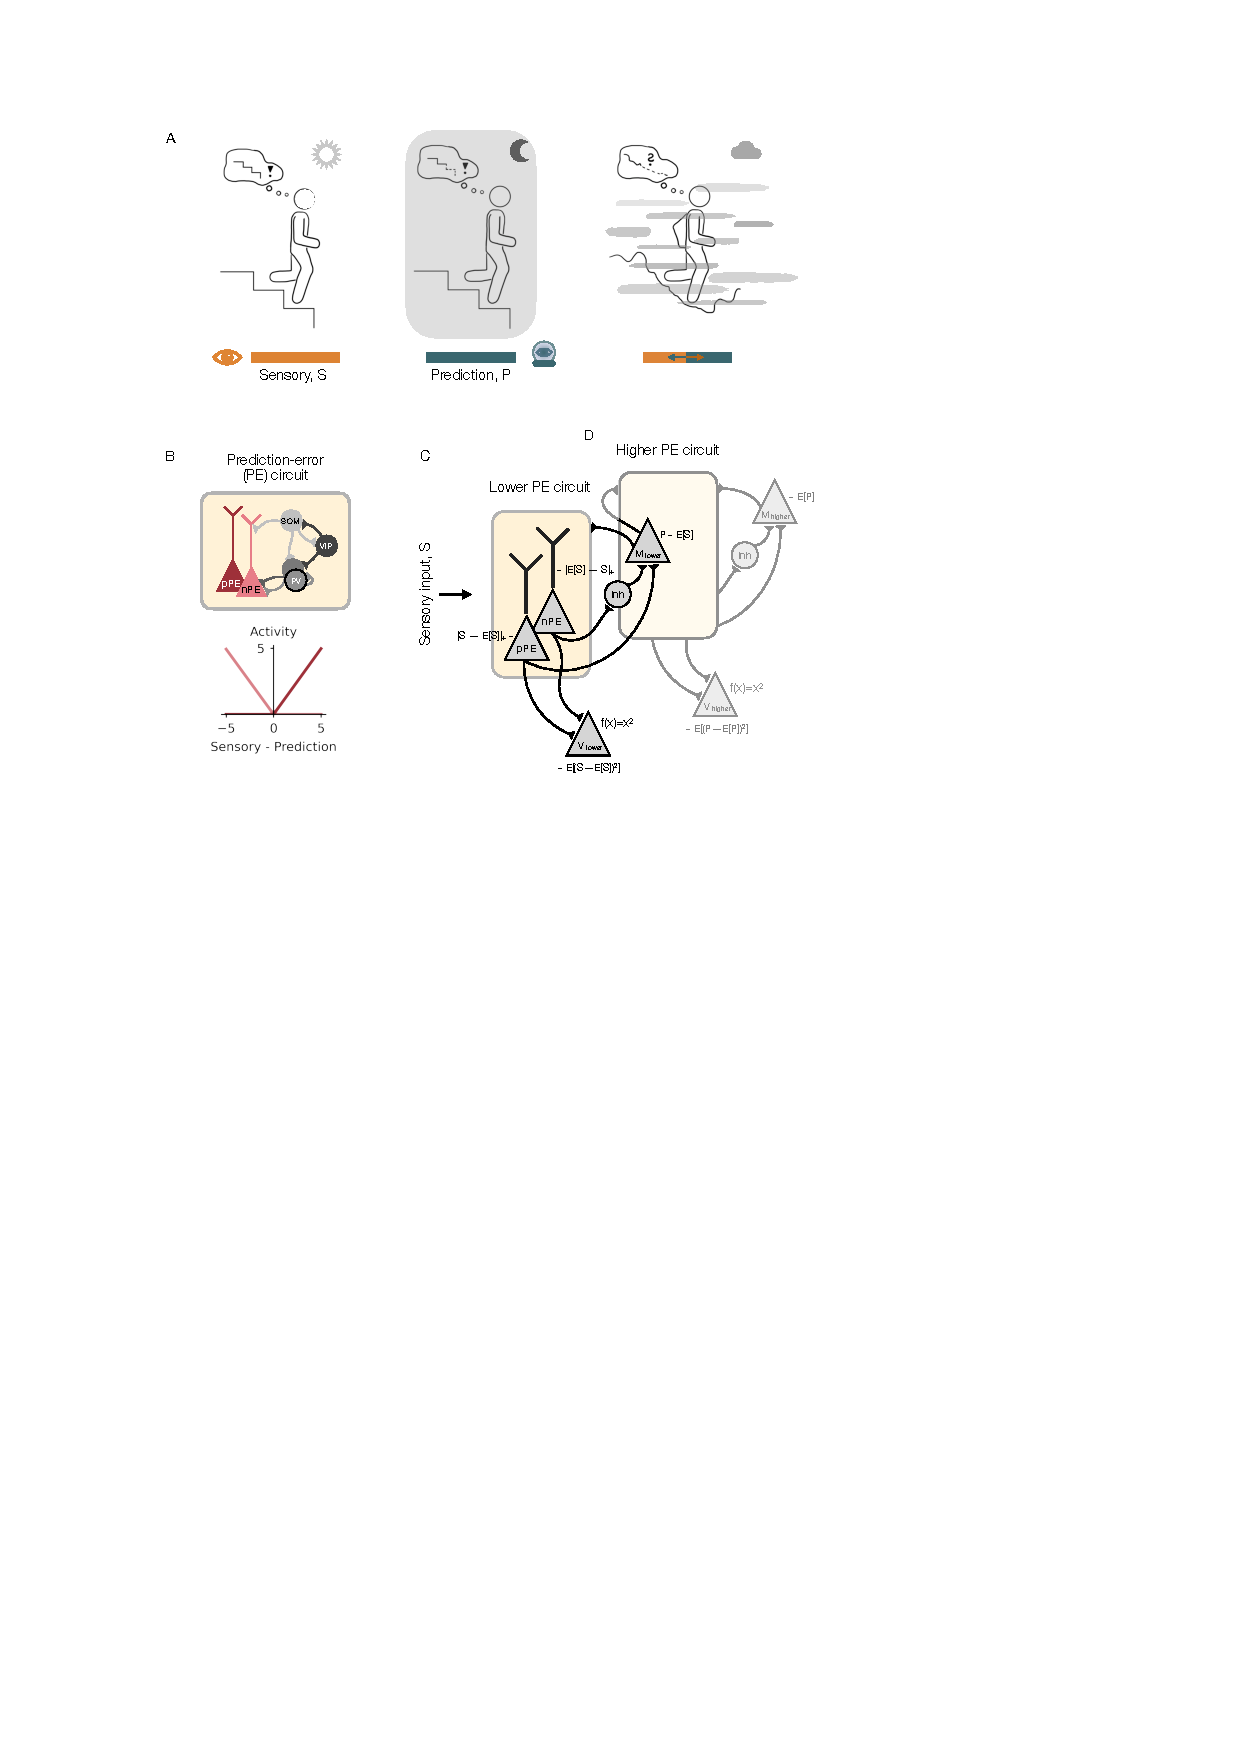
\includegraphics{../results/figures/final/Fig_1}
\caption{\DIFdelbeginFL %DIFDELCMD < \footnotesize{\bf Neural network model to flexibly integrate sensory information and predictions.\newline} 
%DIFDELCMD < %%%
\DIFdelendFL \DIFaddbeginFL \footnotesize{\bf Neural network model to track both the uncertainty of sensory inputs and predictions.\newline} 
\DIFaddendFL {\bf (A)} Example illustration \DIFdelbeginFL \DIFdelFL{of }\DIFdelendFL \DIFaddbeginFL \DIFaddFL{for }\DIFaddendFL context-dependent integration of information. Left: When walking down \DIFdelbeginFL \DIFdelFL{a }\DIFdelendFL \DIFaddbeginFL \DIFaddFL{an unfamiliar }\DIFaddendFL staircase that is \DIFdelbeginFL \DIFdelFL{clearly }\DIFdelendFL visible, the brain might rely solely on external sensory information. Middle: When walking down the same stairs \DIFdelbeginFL \DIFdelFL{in the absence of }\DIFdelendFL \DIFaddbeginFL \DIFaddFL{without }\DIFaddendFL visual information, the brain might rely on predictions formed by previous experience. Right: When climbing down an unexplored mountain in foggy conditions, the brain might need to integrate sensory information and predictions \DIFdelbeginFL \DIFdelFL{at the same time}\DIFdelendFL \DIFaddbeginFL \DIFaddFL{simultaneously}\DIFaddendFL .
{\bf (B)} Illustration of a prediction-error (PE) circuit with both negative and positive PE (nPE/pPE) neurons that receive inhibition from three different inhibitory interneuron types: parvalbumin-expressing (PV), somatostatin-expressing (SOM), and vasoactive intestinal peptide-expressing (VIP) interneurons. Local excitatory connections are not shown for clarity.
{\bf (C)} Illustration of network model that estimates the mean and variance of the external sensory stimuli. The core of this network model is the PE circuit shown in (B). The lower-level V neuron encodes the variance, while the lower-level M neuron encodes the mean of the sensory input.
{\bf (D)} Same as in (C) but the feedforward input is the activity of the lower-level M neuron.
}
\label{fig:Fig_1}
\end{figure}
%


\section*{Results}
%

\subsection*{\DIFdelbegin \DIFdel{nPE and pPE }\DIFdelend \DIFaddbegin \DIFadd{Prediction-error }\DIFaddend neurons as the basis for estimating \DIFaddbegin \DIFadd{the }\DIFaddend mean and variance of sensory stimuli}
%
We \DIFdelbegin \DIFdel{hypothesise }\DIFdelend \DIFaddbegin \DIFadd{hypothesize }\DIFaddend that the distinct response patterns of negative and positive prediction-error (nPE/pPE) neurons \DIFdelbegin \DIFdel{represent the }\DIFdelend \DIFaddbegin \DIFadd{act as a }\DIFaddend backbone for estimating the mean and the variance of sensory stimuli. \DIFdelbegin \DIFdel{nPE neurons only increase their }\DIFdelend \DIFaddbegin \DIFadd{An nPE neuron only increases its }\DIFaddend activity relative to a baseline when the sensory input is weaker than predicted, while \DIFdelbegin \DIFdel{pPE neurons only increase their }\DIFdelend \DIFaddbegin \DIFadd{a pPE neuron only increases its }\DIFaddend activity relative to a baseline when the sensory input is stronger than predicted. Moreover, both nPE and pPE neurons remain at their baseline \DIFdelbegin \DIFdel{activity }\DIFdelend \DIFaddbegin \DIFadd{activities }\DIFaddend when the sensory input is fully predicted (\DIFdelbegin \DIFdel{XXX). Assuming that }\DIFdelend \DIFaddbegin \DIFadd{Fig. \ref{fig:Fig_1}B). If }\DIFaddend the prediction equals the mean of the sensory stimulus, the PE neurons, hence, encode the deviation from the mean. Thus, the squared sum of nPE and pPE neuron activity represents the variance of the feedforward input \DIFaddbegin \DIFadd{(provided that the PE neurons are silent without sensory stimulation)}\DIFaddend .
%
\begin{figure}[t!]
	\centering
	%\makebox[\textwidth][c]{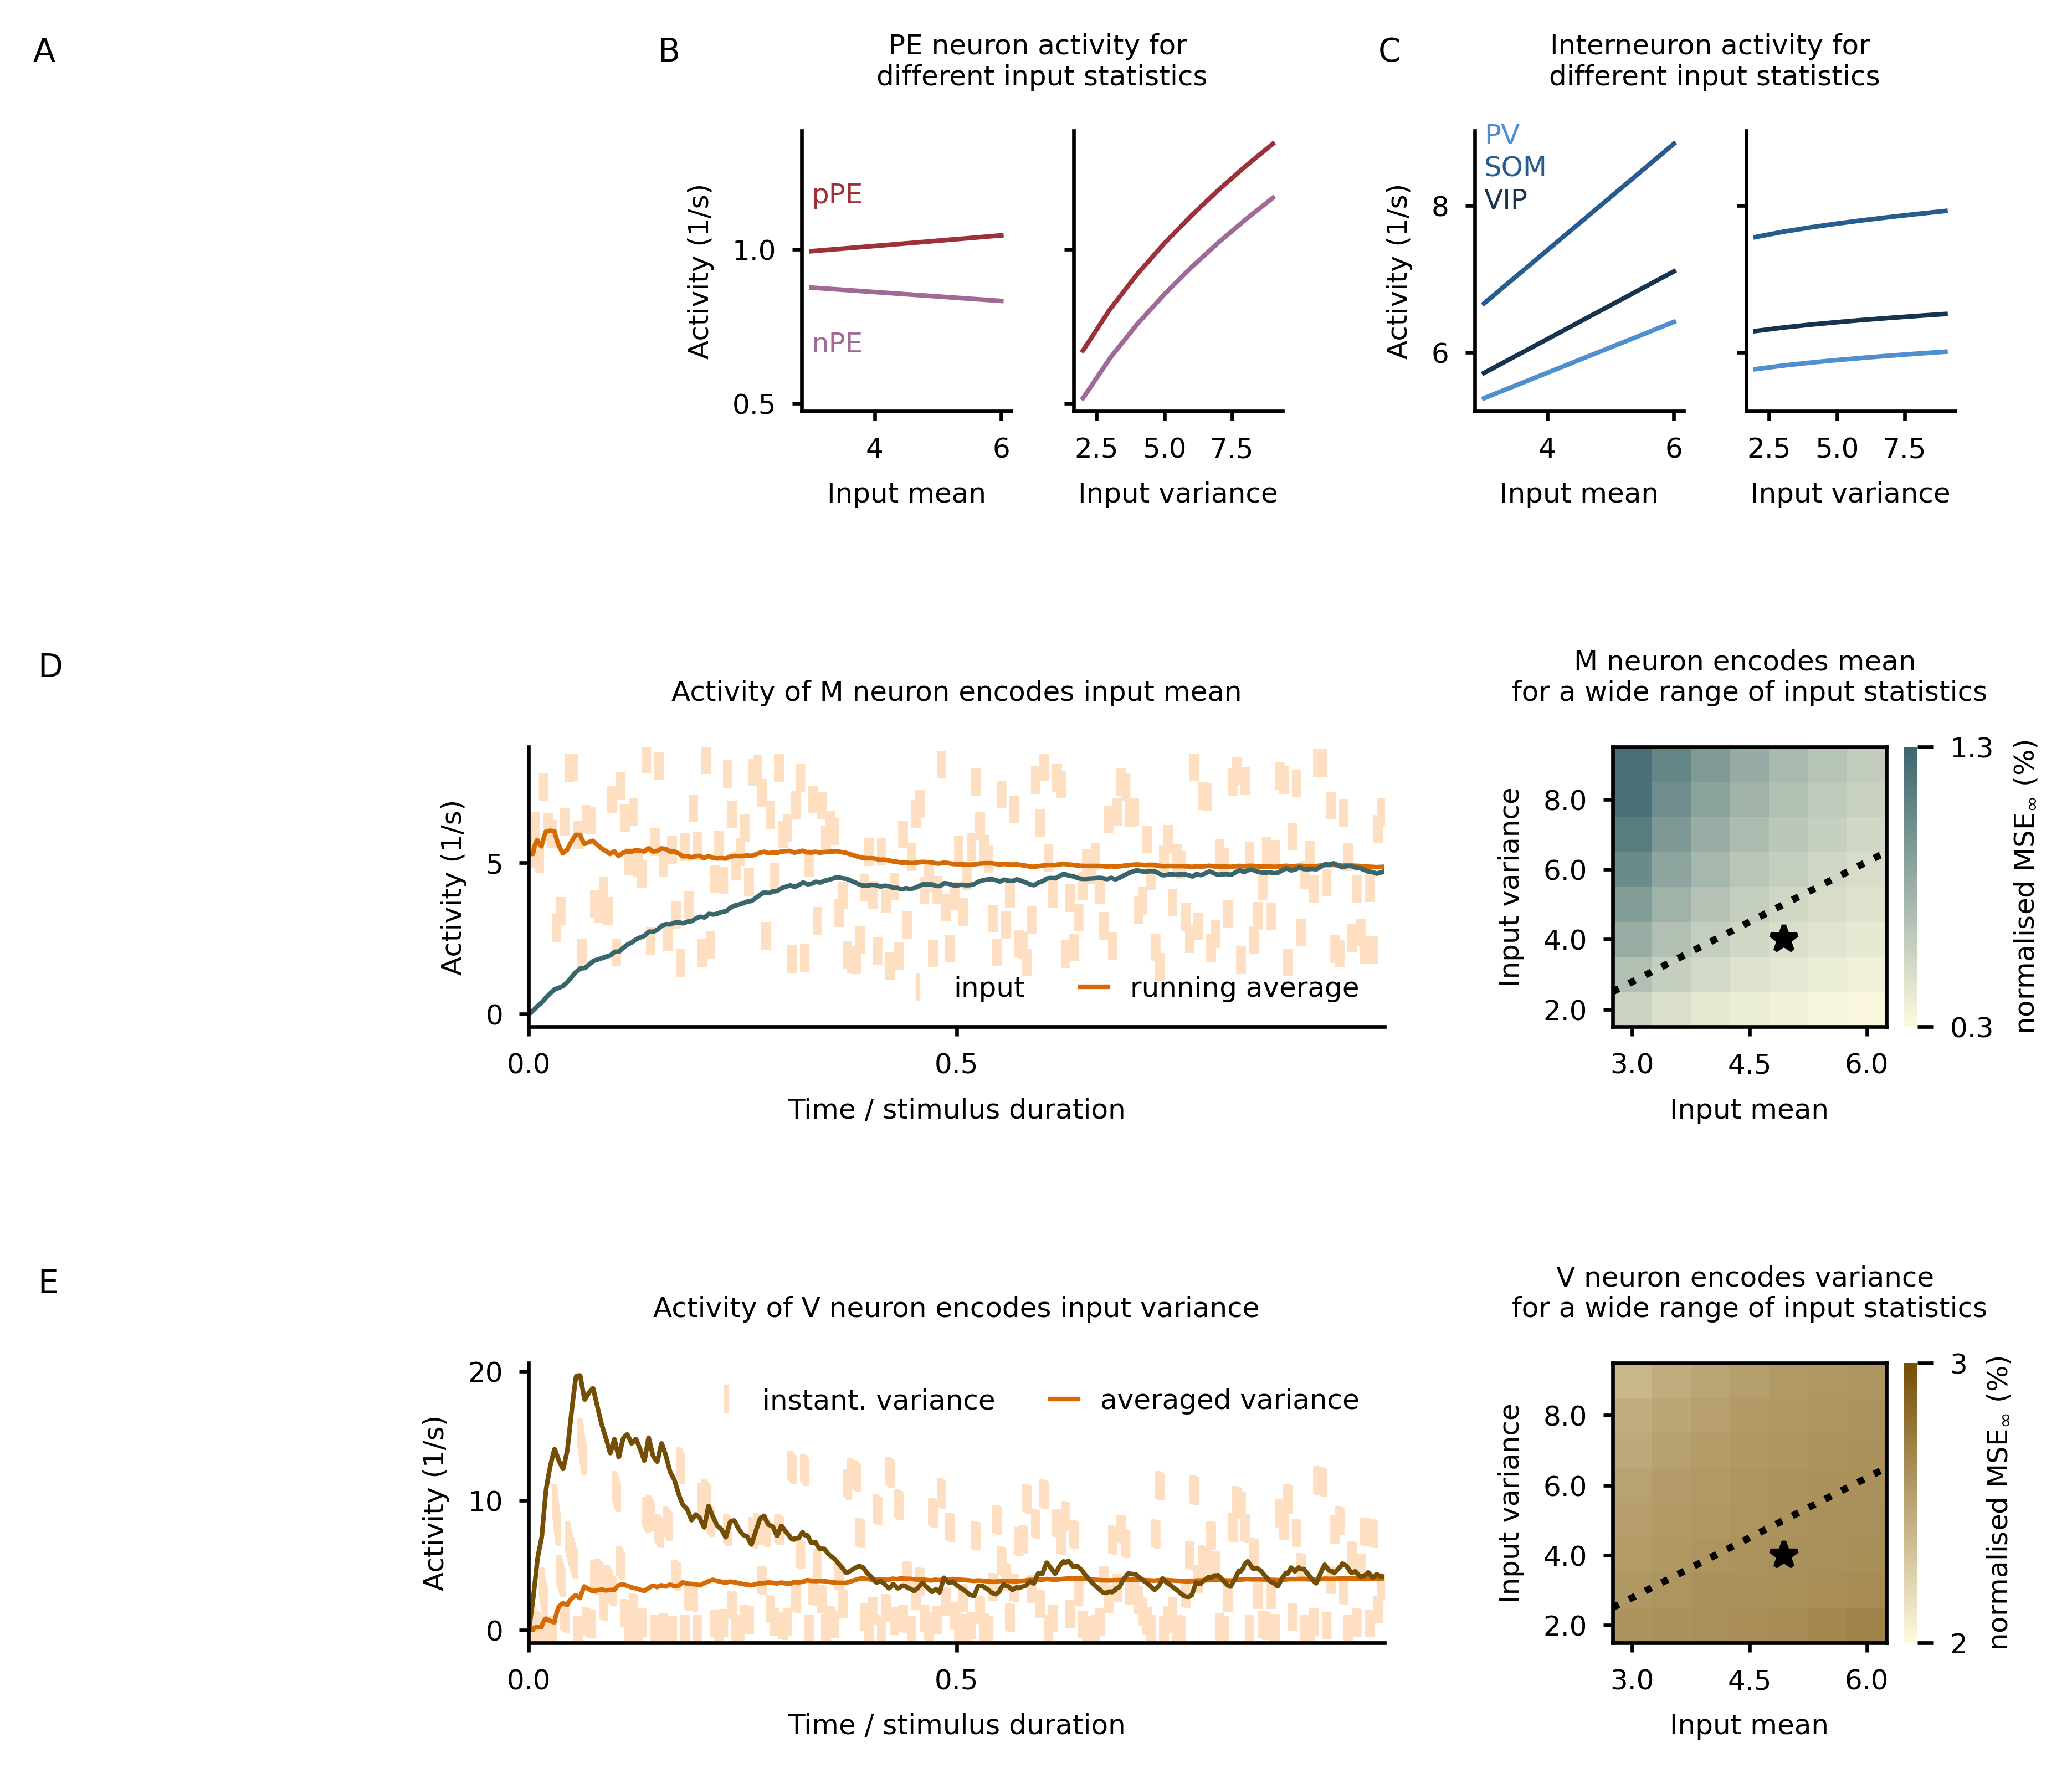
\includegraphics{../results/figures/final/Fig_2}}
    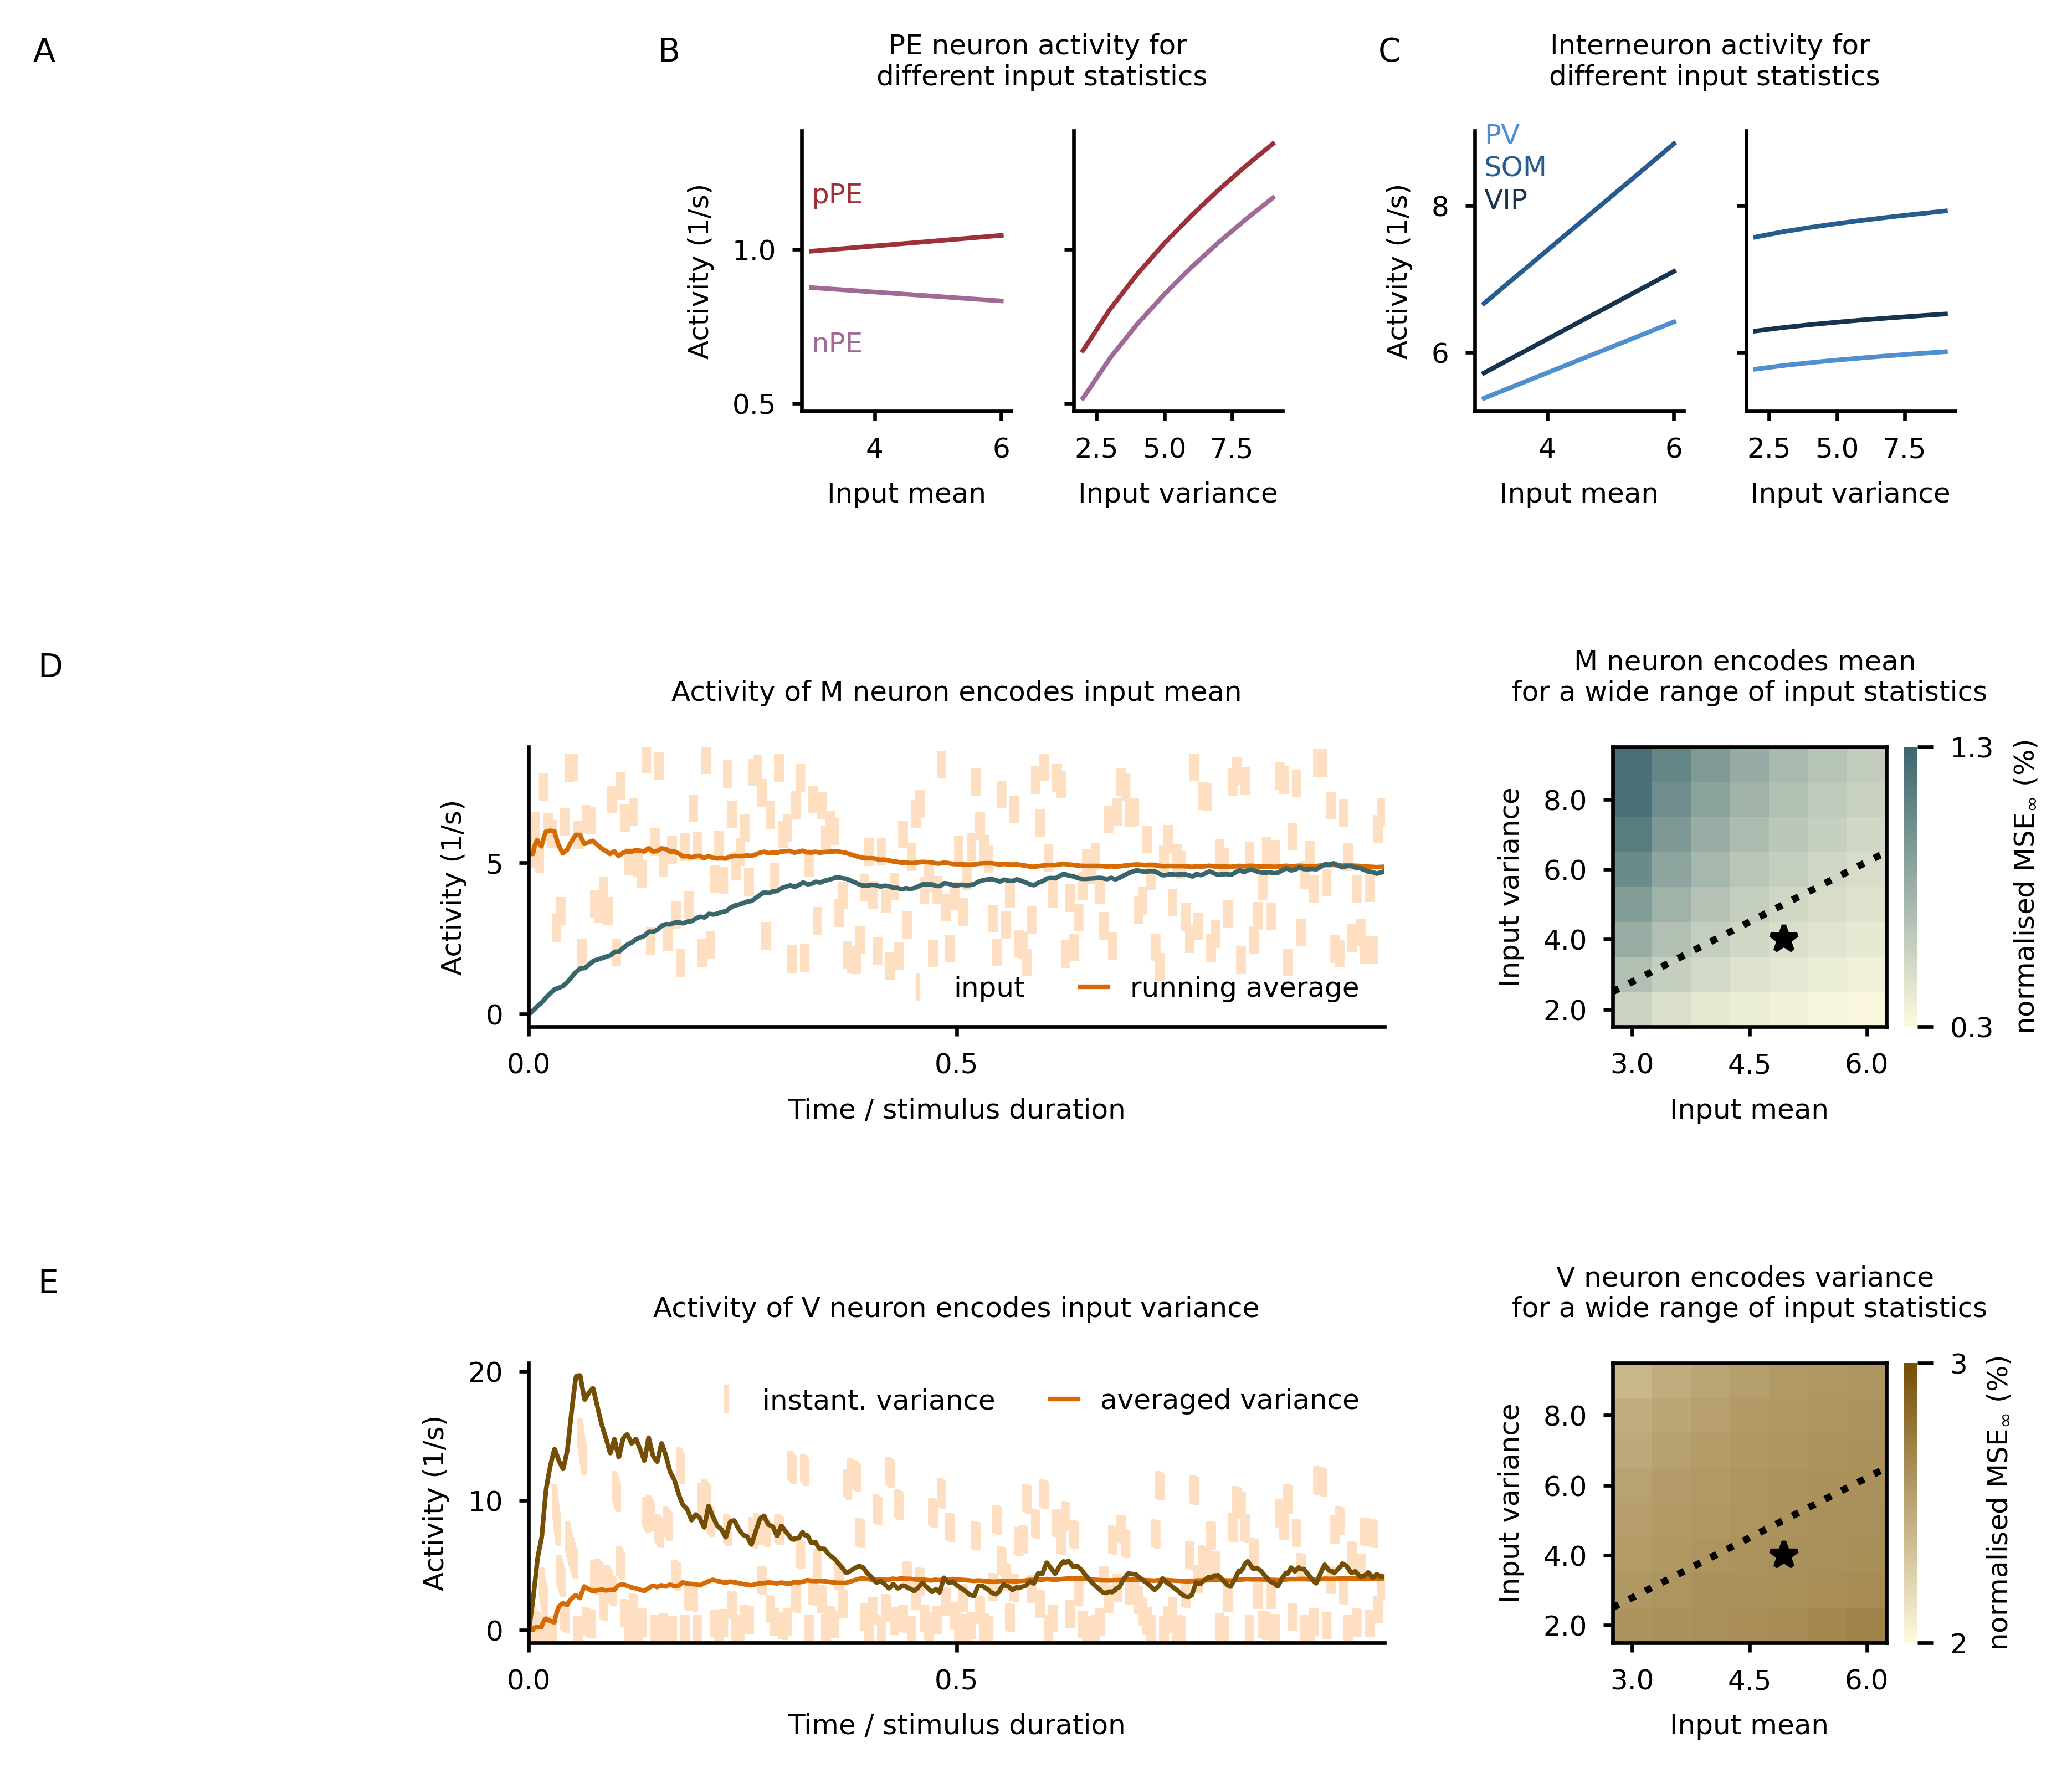
\includegraphics[width=1\linewidth]{../results/figures/final/Fig_2}
\caption{\DIFdelbeginFL %DIFDELCMD < \footnotesize{\bf Prediction-error neurons provide the basis for estimating mean and variance of sensory stimuli.\newline} 
%DIFDELCMD < %%%
\DIFdelendFL \DIFaddbeginFL \footnotesize{\bf Prediction-error neurons as the basis for estimating mean and variance of sensory stimuli.\newline} 
\DIFaddendFL {\bf (A)} Illustration of the inputs with which the network \DIFdelbeginFL \DIFdelFL{shown in }\DIFdelendFL \DIFaddbeginFL \DIFaddFL{(Fig. }\DIFaddendFL \ref{fig:Fig_1}C\DIFaddbeginFL \DIFaddFL{) }\DIFaddendFL is stimulated. Network is exposed to a sequence of constant stimuli drawn from a uniform distribution.
\DIFdelbeginFL \DIFdelFL{Stimulus duration is XXX.
}\DIFdelendFL {\bf (B)} PE neuron activity hardly changes with stimulus strength (left) but strongly increases with stimulus variability (right).
{\bf (C)} Interneuron activity strongly changes with stimulus strength (left) but hardly changes with stimulus variability (right).
{\bf (D)} M neuron correctly encodes the mean of the sensory stimuli. Left: Illustration of the input synapses onto the M neuron. Middle: Activity of the M neuron over time for \DIFdelbeginFL \DIFdelFL{a uniform }\DIFdelendFL \DIFaddbeginFL \DIFaddFL{one example }\DIFaddendFL distribution \DIFdelbeginFL \DIFdelFL{with mean XXX and standard deviation XXX}\DIFdelendFL \DIFaddbeginFL \DIFaddFL{(black start in right panel)}\DIFaddendFL . Right: Normalised \DIFdelbeginFL \DIFdelFL{mean-squared error (MSE) }\DIFdelendFL \DIFaddbeginFL \DIFaddFL{absolute difference }\DIFaddendFL between the \DIFdelbeginFL \DIFdelFL{running average }\DIFdelendFL \DIFaddbeginFL \DIFaddFL{averaged mean }\DIFaddendFL and the \DIFaddbeginFL \DIFaddFL{activity of the }\DIFaddendFL M neuron \DIFdelbeginFL \DIFdelFL{activity }\DIFdelendFL \DIFaddbeginFL \DIFaddFL{in the steady state }\DIFaddendFL for different parametrizations of the stimulus distribution.
{\bf (E)} V neuron correctly encodes the variance of the sensory stimuli. Left: Illustration of the input synapses onto the V neuron. Middle: Activity of the V neuron over time for \DIFdelbeginFL \DIFdelFL{a uniform }\DIFdelendFL \DIFaddbeginFL \DIFaddFL{one example }\DIFaddendFL distribution \DIFdelbeginFL \DIFdelFL{with mean XXX and standard deviation XXX}\DIFdelendFL \DIFaddbeginFL \DIFaddFL{(black start in right panel)}\DIFaddendFL . Right: Normalised \DIFdelbeginFL \DIFdelFL{mean-squared error (MSE) }\DIFdelendFL \DIFaddbeginFL \DIFaddFL{absolute difference }\DIFaddendFL between the \DIFdelbeginFL \DIFdelFL{instantaneous }\DIFdelendFL \DIFaddbeginFL \DIFaddFL{averaged }\DIFaddendFL variance and the \DIFaddbeginFL \DIFaddFL{activity of the }\DIFaddendFL V neuron \DIFdelbeginFL \DIFdelFL{activity }\DIFdelendFL \DIFaddbeginFL \DIFaddFL{in the steady state }\DIFaddendFL for different parametrizations of the stimulus distribution.
}
\label{fig:Fig_2}
\end{figure}
%

To test our hypothesis, we \DIFdelbegin \DIFdel{studied }\DIFdelend \DIFaddbegin \DIFadd{study }\DIFaddend a rate-based mean-field network\DIFdelbegin \DIFdel{the core of which }\DIFdelend \DIFaddbegin \DIFadd{. The core network }\DIFaddend is a prediction-error (PE) circuit with excitatory nPE and pPE neurons, as well as inhibitory parvalbumin-expressing (PV), somatostatin-expressing (SOM), and vasoactive intestinal peptide-expressing (VIP) interneurons (Fig. \ref{fig:Fig_1}B). While the excitatory neurons are simulated as two coupled point compartments to emulate the soma and dendrites of elongated pyramidal cells, respectively, all inhibitory cell types were modeled as point neurons. The connectivity of and inputs to the network were chosen such that the excitatory (E) and inhibitory (I) pathways onto the pyramidal cells were \DIFdelbegin \DIFdel{balanced because it }\DIFdelend \DIFaddbegin \DIFadd{partially balanced. This balance that is only temporarily broken during mismatches }\DIFaddend has been shown \DIFdelbegin \DIFdel{that this E/I balance is }\DIFdelend \DIFaddbegin \DIFadd{to be }\DIFaddend necessary for nPE and pPE neurons to emerge \DIFdelbegin \DIFdel{(XXX, see Methods)}\DIFdelend \DIFaddbegin \DIFadd{\mbox{%DIFAUXCMD
\citep[][see Methods]{hertag2020learning, hertag2022prediction}}\hskip0pt%DIFAUXCMD
}\DIFaddend . 

\DIFdelbegin \DIFdel{In addition to }\DIFdelend \DIFaddbegin \DIFadd{We assume that }\DIFaddend this core circuit \DIFaddbegin \DIFadd{is shaped by feedback connections \mbox{%DIFAUXCMD
\citep{larkum2013cellular, harris2015neocortical} }\hskip0pt%DIFAUXCMD
that have been hypothesized to carry information about expectations or predictions \mbox{%DIFAUXCMD
\citep{mumford1992computational, larkum2013cellular, friston2008hierarchical}}\hskip0pt%DIFAUXCMD
. To account for predictions}\DIFaddend , we model a memory (M) neuron that \DIFdelbegin \DIFdel{perfectly }\DIFdelend integrates the activity of the PE neurons (Fig. \ref{fig:Fig_1}C). \DIFdelbegin \DIFdel{In accordance with XXX}\DIFdelend \DIFaddbegin \DIFadd{Following \mbox{%DIFAUXCMD
\cite{keller2018predictive}}\hskip0pt%DIFAUXCMD
}\DIFaddend , we assume that the pPE neuron excites the memory neuron, while the nPE neuron inhibits this neuron (for instance, through lateral inhibition, here not modeled explicitly). \DIFdelbegin \DIFdel{The M neuron connects to }\DIFdelend \DIFaddbegin \DIFadd{Because feedback connections are shown to target }\DIFaddend the apical dendrites of \DIFdelbegin \DIFdel{the }\DIFdelend \DIFaddbegin \DIFadd{pyramidal cells \mbox{%DIFAUXCMD
\citep{larkum2013cellular} }\hskip0pt%DIFAUXCMD
and interneurons located in superficial layers of the cortex \mbox{%DIFAUXCMD
\citep[see, e.g.][]{tremblay2016gabaergic}}\hskip0pt%DIFAUXCMD
, the M neuron makes connections with the dendritic compartment of the }\DIFaddend PE neurons and some of the interneurons (here, VIP and PV neurons, see Methods for more details). \DIFdelbegin \DIFdel{In this network, the M neuron serves as a prediction that is dynamically updated when new sensory information is available. Wefurthermore }\DIFdelend \DIFaddbegin \DIFadd{We, furthermore, }\DIFaddend simulate a downstream neuron (termed V neuron), modeled as a leaky integrator with a \DIFdelbegin \DIFdel{squared }\DIFdelend \DIFaddbegin \DIFadd{quadratic }\DIFaddend activation function, that receives excitatory \DIFdelbegin \DIFdel{output }\DIFdelend synapses from the PE neurons. Hence, in this setting, the V neuron encodes the variance of the sensory stimuli (Fig. \ref{fig:Fig_1}C). 

To show that this network can indeed represent \DIFdelbegin \DIFdel{mean and }\DIFdelend \DIFaddbegin \DIFadd{the mean and the }\DIFaddend variance in the respective neurons, we stimulate it with a sequence of step-wise constant inputs drawn from a uniform distribution (Fig. \ref{fig:Fig_2}A)\DIFdelbegin \DIFdel{, assuming }\DIFdelend \DIFaddbegin \DIFadd{. We, hence, assume }\DIFaddend that the sensory stimulus varies over time. In line with the distinct response patterns for nPE and pPE neurons, these neurons change only slightly with increasing stimulus mean but increase strongly with input variance (Fig. \ref{fig:Fig_2}B). \DIFdelbegin \DIFdel{This is in contrastto }\DIFdelend \DIFaddbegin \DIFadd{In contrast, }\DIFaddend the three interneurons \DIFdelbegin \DIFdel{that }\DIFdelend strongly increase with stimulus mean \DIFdelbegin \DIFdel{while they }\DIFdelend \DIFaddbegin \DIFadd{and }\DIFaddend only moderately increase with stimulus variance (Fig. \ref{fig:Fig_2}C). The activity of the \DIFdelbegin \DIFdel{memory neuron M }\DIFdelend \DIFaddbegin \DIFadd{M neuron }\DIFaddend gradually approaches the mean of the sensory inputs (Fig. \ref{fig:Fig_2}D, middle), while the activity of the V neuron approaches the variance of \DIFdelbegin \DIFdel{the }\DIFdelend \DIFaddbegin \DIFadd{those }\DIFaddend inputs (Fig. \ref{fig:Fig_2}E, middle). \DIFdelbegin \DIFdel{This is true }\DIFdelend \DIFaddbegin \DIFadd{We show that this holds }\DIFaddend for a wide range of input statistics (Fig. \ref{fig:Fig_2}D-E, right) and input distributions (Fig. \ref{fig:Fig_2_S1}). Small deviations from the true mean occur mainly for \DIFdelbegin \DIFdel{larger }\DIFdelend \DIFaddbegin \DIFadd{large }\DIFaddend input variances, while the estimated variance is fairly independent of the input statistics tested. 

\DIFdelbegin \DIFdel{XXX coming soon: Paragraph on network beyond }\DIFdelend \DIFaddbegin \DIFadd{We verified our results in a heterogeneous network in which a population of neurons represents each neuron type of the PE circuit, and the synaptic connection strengths from each PE neuron onto the M and V neuron are different (see Methods, Fig. \ref{fig:Fig_2_S2}A). As before, the network can correctly estimate the mean and the variance of the sensory stimuli (Fig. \ref{fig:Fig_2_S2}B). Furthermore, we show that the errors with which the M and V neurons encode the stimulus statistics are independent of uncorrelated modulations of those connection strengths (Fig. \ref{fig:Fig_2_S2}C) and the sparsity of the network (Fig. \ref{fig:Fig_2_S2}E). When all connection strengths are collectively shifted to higher values, the error increases for the V neuron, while it remains unaffected for the M neuron. 
}

\DIFadd{While our }\DIFaddend mean-field \DIFdelbegin \DIFdel{XXX
}\DIFdelend \DIFaddbegin \DIFadd{network was designed to track the mean and the variance of stimuli that vary in time, we reasoned that the same principles apply to stimuli that vary across space. To show that, we simulated a population network that consists of unconnected replicates of the mean-field network described above (Fig. \ref{fig:Fig_2_S3}A). Each mean-field network receives a short, constant input from a different part of the receptive field. If the connection strengths from the PE neurons to the M and V neurons are adjusted accordingly (see Methods), the network correctly estimates the stimulus average and spatial uncertainty. (Fig. \ref{fig:Fig_2_S3}B-C).
}\DIFaddend 

In summary, nPE and pPE neurons can \DIFdelbegin \DIFdel{be the }\DIFdelend \DIFaddbegin \DIFadd{serve as a }\DIFaddend basis to estimate the mean and the variance of sensory stimuli \DIFdelbegin \DIFdel{that }\DIFdelend \DIFaddbegin \DIFadd{which }\DIFaddend vary over time \DIFaddbegin \DIFadd{and space}\DIFaddend .


\subsection*{Estimating \DIFdelbegin \DIFdel{variances }\DIFdelend \DIFaddbegin \DIFadd{the uncertainty }\DIFaddend of \DIFaddbegin \DIFadd{both the }\DIFaddend sensory \DIFdelbegin \DIFdel{inputs }\DIFdelend \DIFaddbegin \DIFadd{input }\DIFaddend and \DIFdelbegin \DIFdel{predictions }\DIFdelend \DIFaddbegin \DIFadd{the prediction }\DIFaddend requires a hierarchy of PE circuits}
%
Following the ideas of Bayesian multisensory integration\DIFdelbegin \DIFdel{(XXX)}\DIFdelend , the weighting of sensory stimuli and predictions \DIFdelbegin \DIFdel{thereof }\DIFdelend would require knowledge \DIFdelbegin \DIFdel{of their variances}\DIFdelend \DIFaddbegin \DIFadd{about their uncertainties}\DIFaddend . As we have shown in the previous section, the variance of the sensory stimulus can be estimated using PE neurons. We \DIFdelbegin \DIFdel{hypothesise }\DIFdelend \DIFaddbegin \DIFadd{hypothesize }\DIFaddend that the same principles apply to computing the variance of the prediction. Hence, we augment the network with a \textit{higher} PE circuit that receives \DIFdelbegin \DIFdel{output }\DIFdelend \DIFaddbegin \DIFadd{feedforward }\DIFaddend synapses from the M neuron of the \textit{lower} PE circuit (Fig. \ref{fig:Fig_1}D). Both subnetworks are \DIFdelbegin \DIFdel{modeled the same, except that }\DIFdelend \DIFaddbegin \DIFadd{identical except for }\DIFaddend the M neuron in the higher PE circuit \DIFdelbegin \DIFdel{evolves more slowly }\DIFdelend \DIFaddbegin \DIFadd{which is modeled with slower dynamics }\DIFaddend than the one in the lower PE circuit.
%
\begin{figure}[t!]
	\centering
	%\makebox[\textwidth][c]{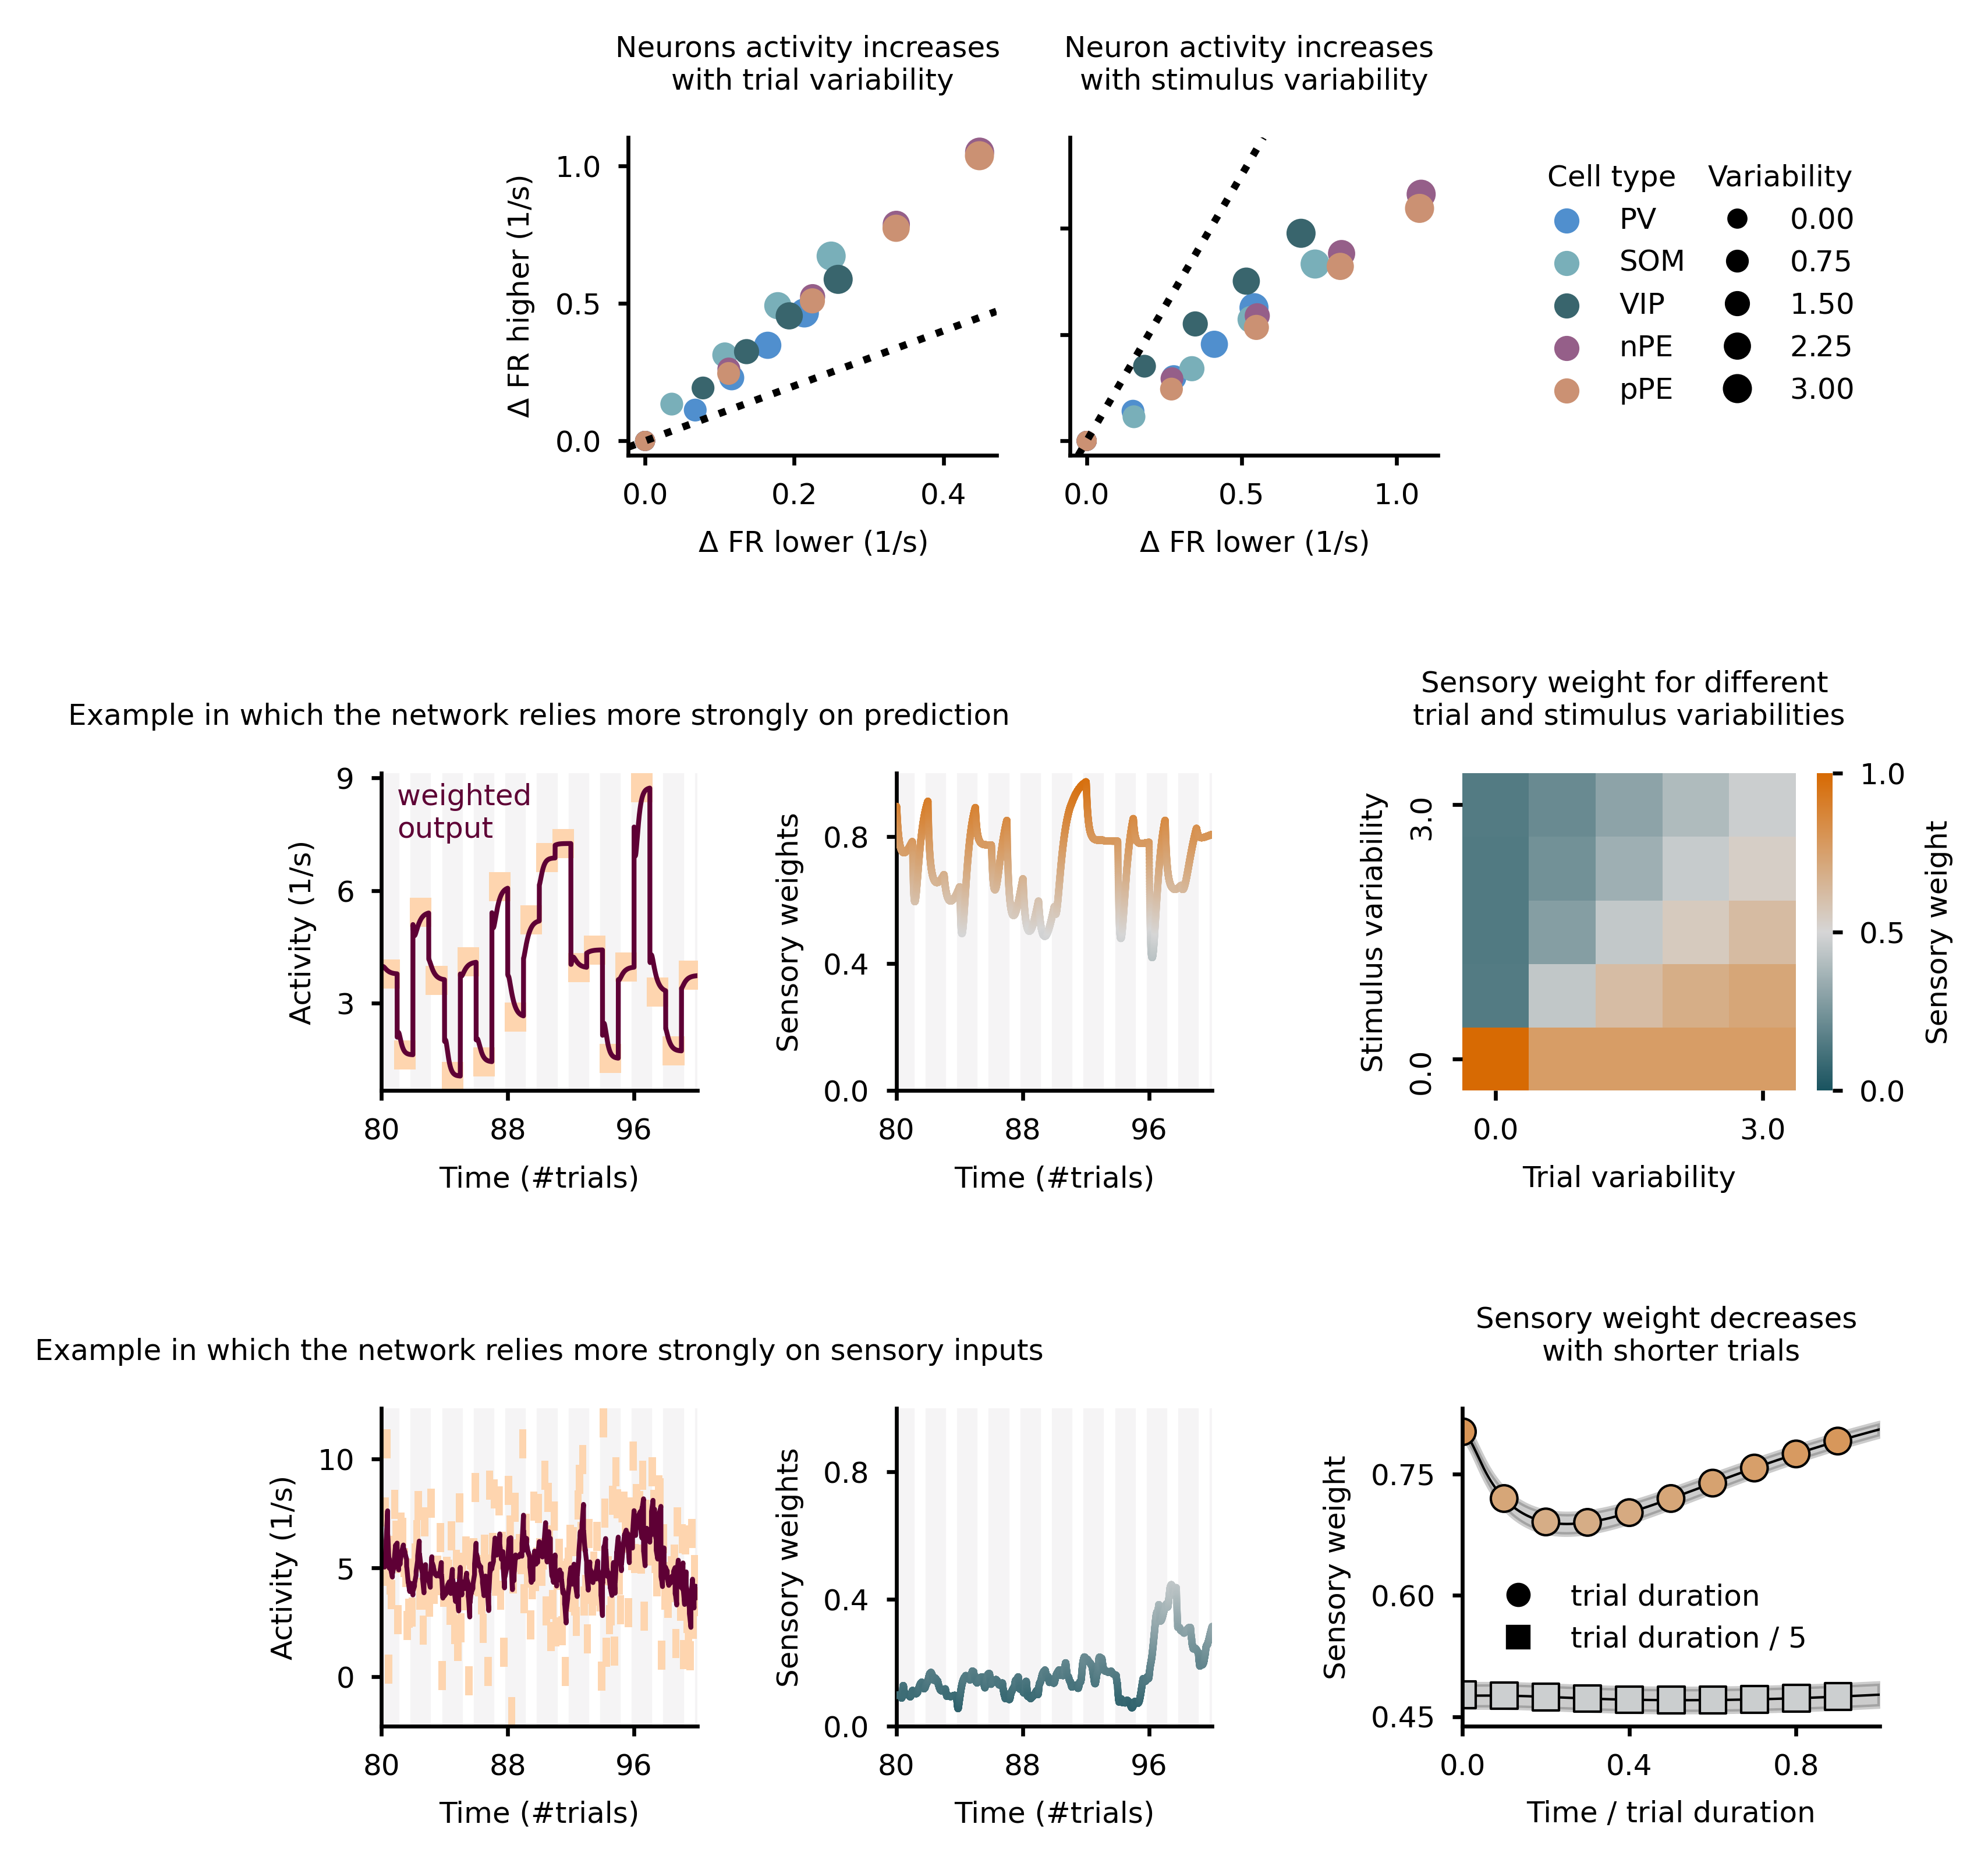
\includegraphics{../results/figures/final/Fig_3}}
    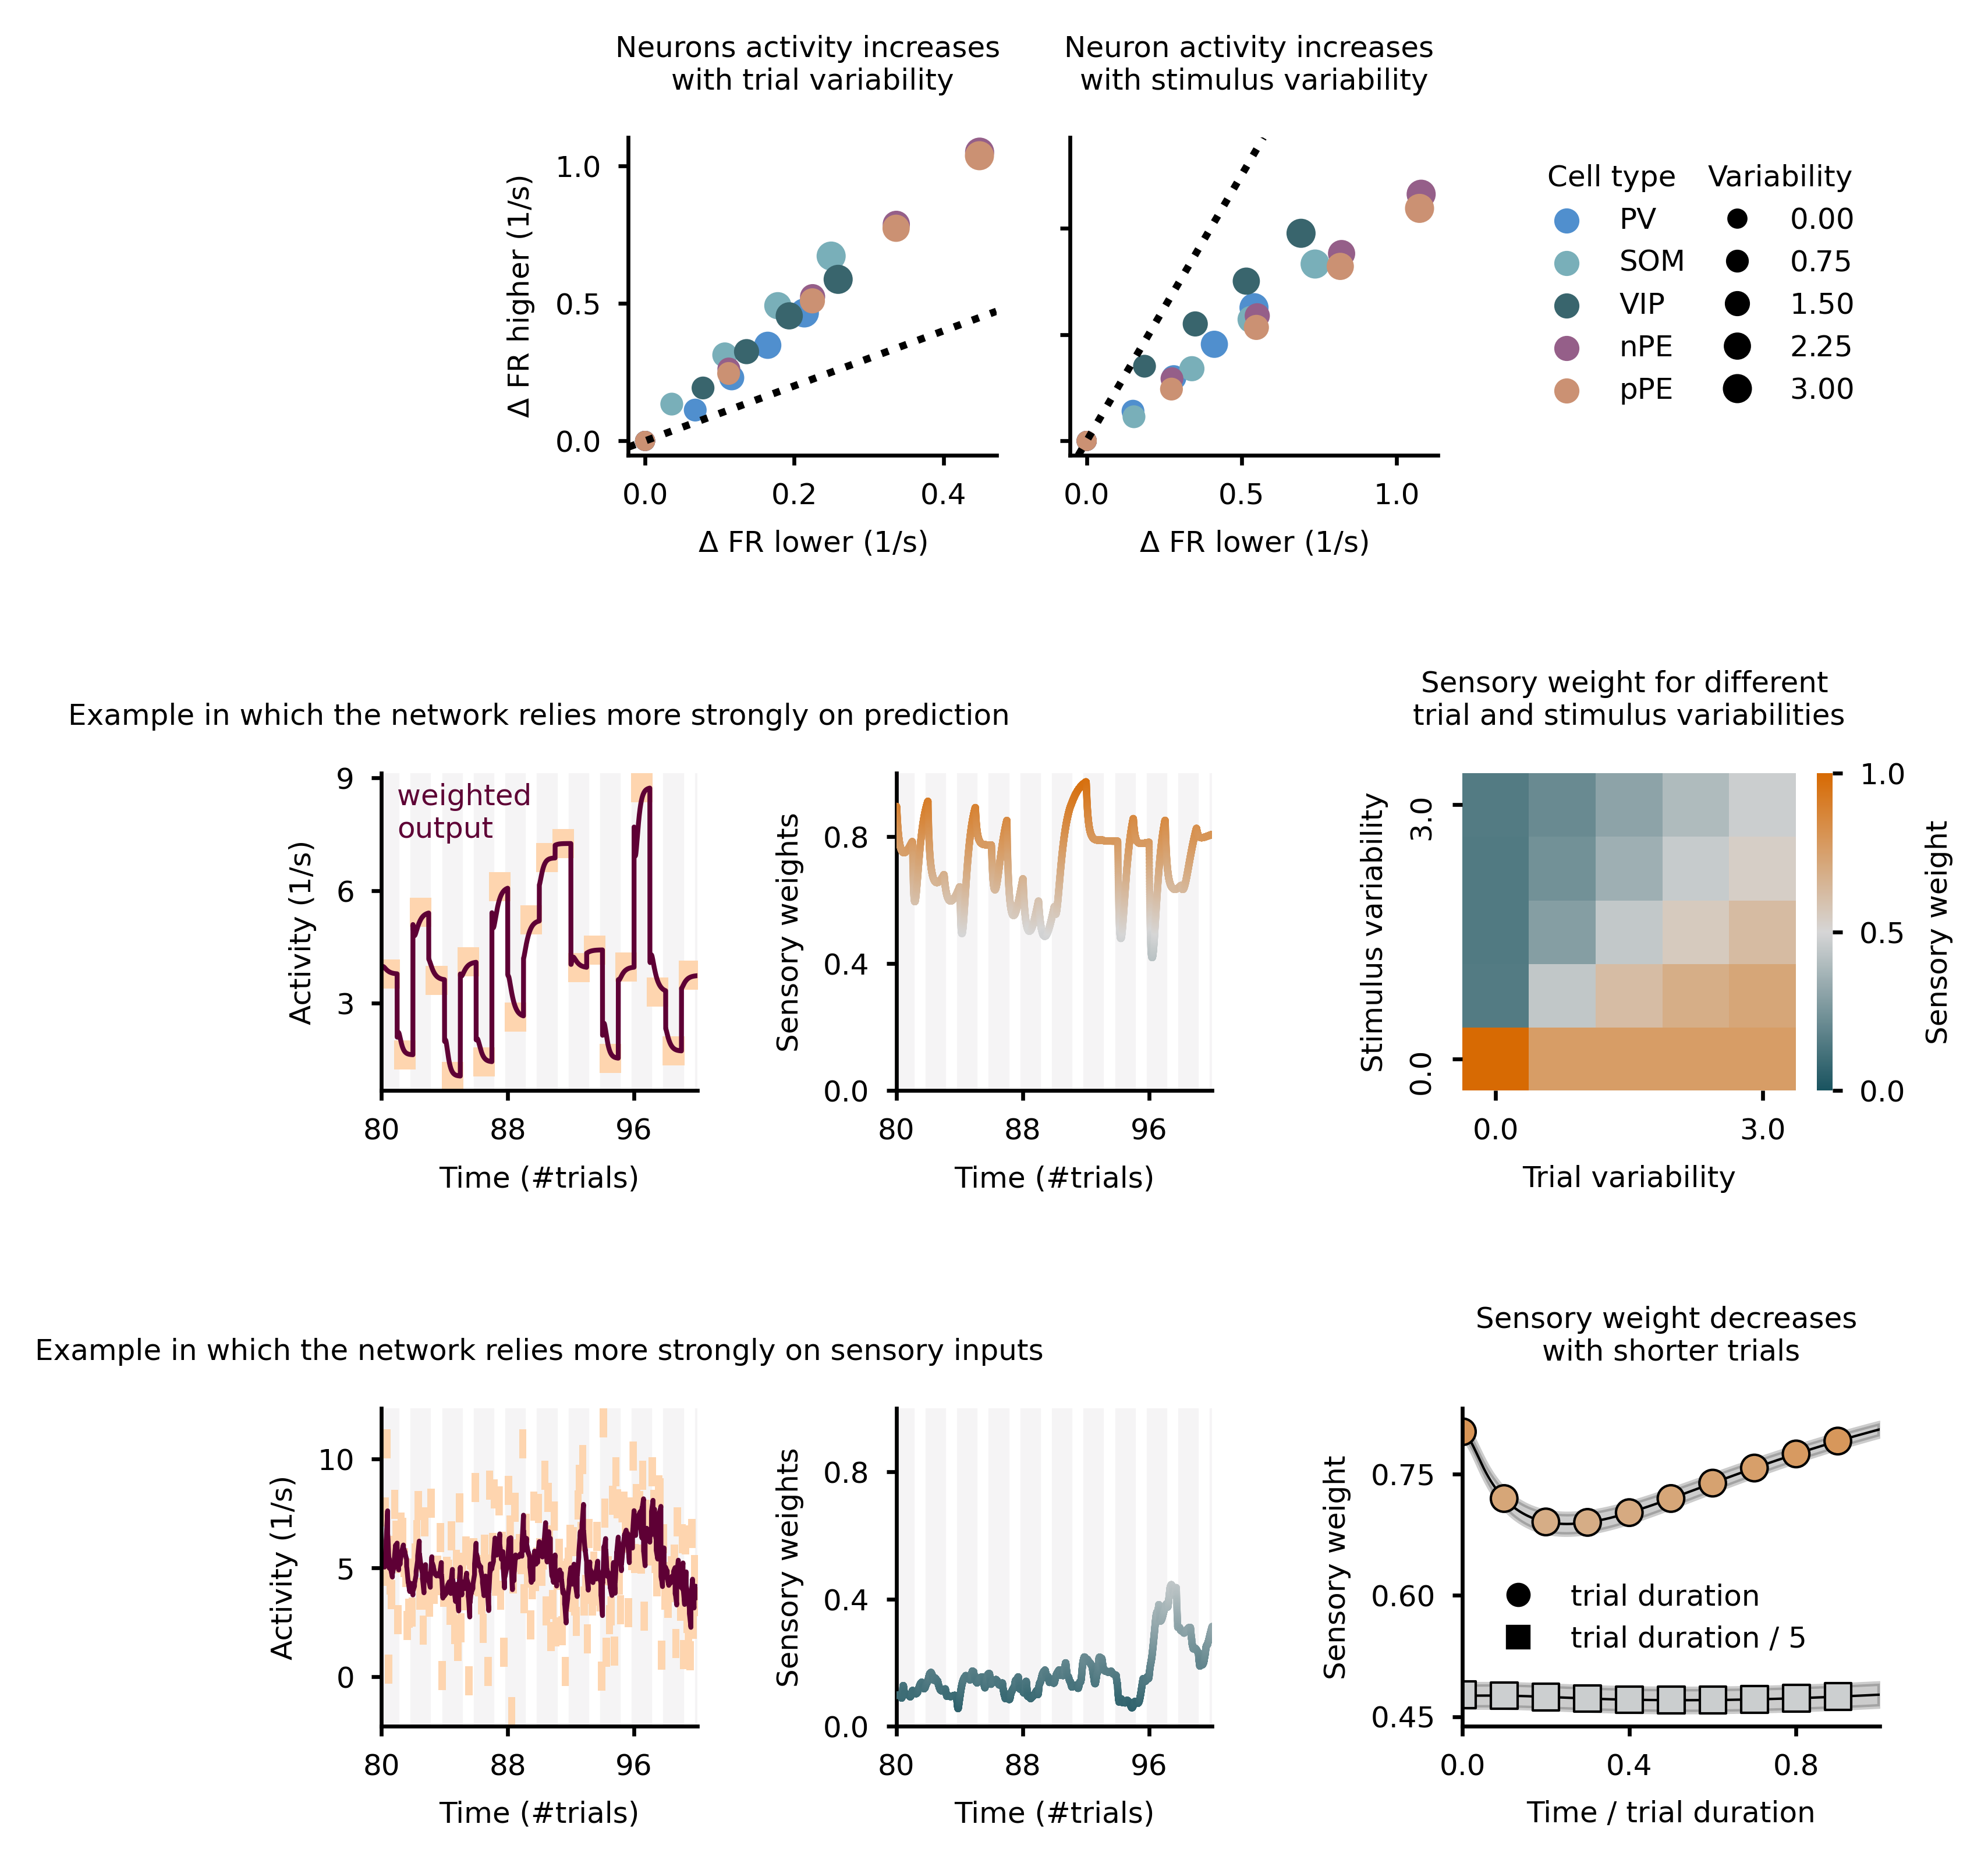
\includegraphics[width=1\linewidth]{../results/figures/final/Fig_3}
\caption{\DIFdelbeginFL %DIFDELCMD < \footnotesize{\bf Estimating variances of sensory inputs and predictions with hierarchical PE circuits.\newline} 
%DIFDELCMD < %%%
\DIFdelendFL \DIFaddbeginFL \footnotesize{\bf Estimating the uncertainty of both the sensory input and the prediction.\newline} 
\DIFaddendFL {\bf (A)} Illustration of the stimulation protocol. \DIFdelbeginFL \DIFdelFL{Network }\DIFdelendFL \DIFaddbeginFL \DIFaddFL{The network }\DIFaddendFL is exposed to a sequence of stimuli (one stimulus per trial). To account for stimulus variability, each stimulus is represented by \DIFdelbeginFL \DIFdelFL{xxx }\DIFdelendFL \DIFaddbeginFL \DIFaddFL{$10$ }\DIFaddendFL stimulus values drawn from a normal distribution\DIFdelbeginFL \DIFdelFL{with mean $\mu_\mathrm{stim}$ and $\sigma_\mathrm{stim}^2$}\DIFdelendFL . To account for the volatility of the environment, in each trial\DIFaddbeginFL \DIFaddFL{, }\DIFaddendFL the stimulus mean \DIFdelbeginFL \DIFdelFL{$\mu_\mathrm{stim}$ }\DIFdelendFL is drawn from a uniform distribution (denoted trial variability). 
\DIFdelbeginFL \DIFdelFL{Trial duration = xxx. 
}\DIFdelendFL {\bf (B)} \DIFdelbeginFL \DIFdelFL{Neuron activity increases with both stimulus and trial variability. Neurons in }\DIFdelendFL \DIFaddbeginFL \DIFaddFL{Illustration of how }\DIFaddendFL the \DIFdelbeginFL \DIFdelFL{lower PE circuit increase more strongly with stimulus variability}\DIFdelendFL \DIFaddbeginFL \DIFaddFL{weighted output is calculated}\DIFaddendFL . \DIFdelbeginFL \DIFdelFL{Neurons in }\DIFdelendFL \DIFaddbeginFL \DIFaddFL{The sensory weight $\alpha$ lies between zero (system relies perfectly on prediction) and one (system relies solely on }\DIFaddendFL the \DIFdelbeginFL \DIFdelFL{higher PE circuit increase more strongly with trial variability}\DIFdelendFL \DIFaddbeginFL \DIFaddFL{sensory input)}\DIFaddendFL .
{\bf (C)} Limit case example in which the stimulus variability is \DIFdelbeginFL \DIFdelFL{low }\DIFdelendFL \DIFaddbeginFL \DIFaddFL{zero }\DIFaddendFL but the trial variability is high. Left: Illustration of the stimulation protocol. Middle: Weighted output follows closely the sensory stimuli. Right: Sensory weight (function of the variances, see \DIFdelbeginFL \DIFdelFL{text}\DIFdelendFL \DIFaddbeginFL \DIFaddFL{B}\DIFaddendFL ) close to 1, indicating that the network ignores the prediction. Input statistics \DIFdelbeginFL \DIFdelFL{: XXX}\DIFdelendFL \DIFaddbeginFL \DIFaddFL{shown in E}\DIFaddendFL .
{\bf (D)} Limit case example in which the stimulus variability is high but the trial variability is \DIFdelbeginFL \DIFdelFL{low}\DIFdelendFL \DIFaddbeginFL \DIFaddFL{zero}\DIFaddendFL . Left: Illustration of the stimulation protocol. Middle: Weighted output pushed towards the mean of the sensory stimuli. Right: Sensory weight close to zero, indicating that the network ignores the sensory stimuli. Input statistics \DIFdelbeginFL \DIFdelFL{: XXX}\DIFdelendFL \DIFaddbeginFL \DIFaddFL{shown in E}\DIFaddendFL .
{\bf (E)} \DIFaddbeginFL \DIFaddFL{Sensory weight for different input statistics. }\DIFaddendFL Predictions are weighted more strongly when the stimulus variability is larger than the trial variability.
{\bf (F)} \DIFaddbeginFL \DIFaddFL{Sensory weight throughout a trial for two different trial durations. }\DIFaddendFL Predictions are weighted more strongly at the beginning of a new trial\DIFdelbeginFL \DIFdelFL{and quickly changing stimuli}\DIFdelendFL . 
}
\label{fig:Fig_3}
\end{figure}
%

To test the network's ability to estimate the variances correctly, we stimulated the network with a sequence of inputs \DIFdelbegin \DIFdel{. In each trialone stimulus is shown to the network . To account for the stimulus variance, each stimulus }\DIFdelend \DIFaddbegin \DIFadd{whose mean can vary from trial to trial. More precisely, in each trial, the network is presented with a stimulus that }\DIFaddend is composed of \textit{n} constant\DIFaddbegin \DIFadd{, consecutive }\DIFaddend values drawn from a normal distribution\DIFdelbegin \DIFdel{with mean $\mu_\mathrm{stim}$ and variance $\sigma_\mathrm{stim}^2$, and presented one after the other}\DIFdelend \DIFaddbegin \DIFadd{. The variance of this distribution represents the stimulus noise}\DIFaddend . To account for potential changes in the environment, \DIFdelbegin \DIFdel{in each trial, we draw $\mu_\mathrm{stim}$ }\DIFdelend \DIFaddbegin \DIFadd{we draw the stimulus mean }\DIFaddend from a uniform distribution (Fig. \ref{fig:Fig_3}A). Hence, the inputs change on two different time scales, \DIFdelbegin \DIFdel{with stimulus variability (}\DIFdelend \DIFaddbegin \DIFadd{where the stimulus variability has a }\DIFaddend faster time scale \DIFdelbegin \DIFdel{) and trial variability(slower time scale)}\DIFdelend \DIFaddbegin \DIFadd{than the trial variability}\DIFaddend .

\DIFdelbegin \DIFdel{As expected, the neurons'activity increase for both stimulus and trial variances (Fig. \ref{fig:Fig_3}B). While the neurons in the lower PE circuit increase more strongly with stimulus variability, the neurons in the higher PE circuit increase more strongly with trial variability, indicating that the different subnetworks process different aspects of the inputs. We }\DIFdelend \DIFaddbegin \DIFadd{Following the formalism of multisensory integration \mbox{%DIFAUXCMD
\citep[see, e.g.][]{pouget2013probabilistic}}\hskip0pt%DIFAUXCMD
, we assume that the network's output is a weighted sum of the feedforward sensory input and the feedback prediction. The weights assigned to each input stream are functions of the uncertainties, that is, the activities of the V neurons. The sensory weight captures, hence, how much the network relies on the sensory input (Fig. \ref{fig:Fig_2}B). To test our network, we }\DIFaddend first consider two limit cases. In the first limit case, a different\DIFdelbegin \DIFdel{but }\DIFdelend \DIFaddbegin \DIFadd{, }\DIFaddend low-variance stimulus is presented in each trial (Fig. \ref{fig:Fig_3}C, left). \DIFdelbegin \DIFdel{In line with the ideas of multisensory integration (XXX)}\DIFdelend \DIFaddbegin \DIFadd{According to the theory}\DIFaddend , the network should \DIFdelbegin \DIFdel{therefore }\DIFdelend follow the sensory inputs closely and ignore the predictions. When we arithmetically calculate the weighted output (Fig. \ref{fig:Fig_3}C, middle) \DIFdelbegin \DIFdel{based on the feedforward and feedback inputs, and }\DIFdelend \DIFaddbegin \DIFadd{and }\DIFaddend the sensory weight (Fig. \ref{fig:Fig_3}C, right), the network \DIFdelbegin \DIFdel{correctly represents mostly }\DIFdelend \DIFaddbegin \DIFadd{indeed shows a clear preference for }\DIFaddend the sensory input\DIFdelbegin \DIFdel{(for more details, see Methods)}\DIFdelend . In the second limit case, the same\DIFdelbegin \DIFdel{but }\DIFdelend \DIFaddbegin \DIFadd{, }\DIFaddend high-variance stimulus is presented in each trial (Fig. \ref{fig:Fig_3}D, left). According to the theory, the network should downscale the sensory feedforward input and weight the prediction more strongly. Indeed, the weighted output of the network shows a clear tendency to the mean of the stimuli (Fig. \ref{fig:Fig_3}D, middle), also reflected in the low sensory weight (Fig. \ref{fig:Fig_3}D, right). 

\DIFdelbegin \DIFdel{In a next step, to }\DIFdelend \DIFaddbegin \DIFadd{To }\DIFaddend validate the network responses \DIFdelbegin \DIFdel{more broadly}\DIFdelend \DIFaddbegin \DIFadd{fully}\DIFaddend , we systematically varied the trial and stimulus variability independently. If both variances are similar, the sensory weight approaches \textit{0.5}, reflecting equal contribution of \DIFdelbegin \DIFdel{sensory inputs and predictions }\DIFdelend \DIFaddbegin \DIFadd{the sensory input and the prediction }\DIFaddend to the weighted output. Only if both variances are zero, the network represents the sensory input perfectly. In line with the limit case examples above, if the stimulus variance is larger than the trial variance, the network weights the prediction more strongly than the sensory input \DIFdelbegin \DIFdel{. This is reversed if the stimulus variance is smaller than the trial variance }\DIFdelend (Fig. \ref{fig:Fig_3}E). Because the network dynamically estimates the \DIFdelbegin \DIFdel{mean and variances of the sensory input and the prediction , the weighted output and the }\DIFdelend sensory \DIFaddbegin \DIFadd{and prediction uncertainty, the sensory }\DIFaddend weight changes \DIFdelbegin \DIFdel{accordingly }\DIFdelend when the input statistics \DIFdelbegin \DIFdel{changes }\DIFdelend \DIFaddbegin \DIFadd{shifts }\DIFaddend (Fig. \ref{fig:Fig_3_S1}). 

\DIFdelbegin \DIFdel{The first limit case (Fig. \ref{fig:Fig_3}C) shows that even in a sensory-driven input regime, }\DIFdelend \DIFaddbegin \DIFadd{Inspecting closely the dynamics of our network, we noticed that }\DIFaddend the prediction is \DIFdelbegin \DIFdel{weighted more }\DIFdelend \DIFaddbegin \DIFadd{typically weighted higher }\DIFaddend at the beginning of a new trial than in the steady state. This is \DIFaddbegin \DIFadd{particularly pronounced in a sensory-driven input regime (see Fig. \ref{fig:Fig_3}C). This is }\DIFaddend further confirmed in simulations in which the trail duration was shortened \DIFdelbegin \DIFdel{. For those simulations, the prediction even outweighs the sensory input, reflected in a very low sensory weight }\DIFdelend (Fig. \ref{fig:Fig_3}F). \DIFdelbegin \DIFdel{This suggests that }\DIFdelend \DIFaddbegin \DIFadd{Our model makes therefore the following experimentally testable prediction: Sensory }\DIFaddend predictions influence neural activity more significantly in experiments that rely on \DIFdelbegin \DIFdel{very }\DIFdelend fast stimulus changes. 

It has been \DIFdelbegin \DIFdel{shown }%DIFDELCMD < [%%%
\DIFdel{speculated?}%DIFDELCMD < ]%%%
\DIFdel{, that sensory inputs or predictions are overrated in some psychiatric disorders (XXX)}\DIFdelend \DIFaddbegin \DIFadd{hypothesized, that some symptoms in psychiatric disorders like autism and schizophrenia can be ascribed to a pathological weighting of sensory inputs and predictions \mbox{%DIFAUXCMD
\citep{yon2021precision}}\hskip0pt%DIFAUXCMD
}\DIFaddend . We thus wondered which network properties might bias the estimation of the variances, and, consequently, the weighting of different input streams. \DIFdelbegin \DIFdel{In our network, the M neuron evolves faster in the lower subnetwork than in the higher one. }\DIFdelend We identified the \DIFdelbegin \DIFdel{speed }\DIFdelend \DIFaddbegin \DIFadd{time scales }\DIFaddend at which the M neurons \DIFdelbegin \DIFdel{are updated with }\DIFdelend \DIFaddbegin \DIFadd{incorporate }\DIFaddend new information as a decisive factor in the integration of inputs. To show this, we varied the weights from the PE neurons onto the lower-level M neuron. If the \DIFdelbegin \DIFdel{M neuron evolves too slowly, the prediction is overrated}\DIFdelend \DIFaddbegin \DIFadd{weights are too small (M updates too slowly), the system relies too much on feedback predictions}\DIFaddend . In contrast, if the \DIFdelbegin \DIFdel{M neuron incorporates new information too quickly, the sensory input is overrated }\DIFdelend \DIFaddbegin \DIFadd{weights are too large (M updates too fast), the system relies too much on the feedforward sensory information }\DIFaddend (Fig. \ref{fig:Fig_3_S2}A). While the speeds at which the activity of the M neurons evolve \DIFdelbegin \DIFdel{may underlie pathological }\DIFdelend \DIFaddbegin \DIFadd{influence the }\DIFaddend weighting of inputs, the precise activation function of the V neurons is less pivotal. When we replaced the \DIFdelbegin \DIFdel{squared }\DIFdelend \DIFaddbegin \DIFadd{quadratic }\DIFaddend activation function with a linear, rectified function, the V neurons \DIFdelbegin \DIFdel{do }\DIFdelend \DIFaddbegin \DIFadd{did }\DIFaddend not encode the variance but the \DIFdelbegin \DIFdel{averaged }\DIFdelend \DIFaddbegin \DIFadd{average }\DIFaddend absolute deviation of the sensory stimuli. However, the sensory weight is only slightly shifted to larger values for low trial/high stimulus variability (Fig. \ref{fig:Fig_3_S2}B). 

In summary, we show that the variances of both the sensory inputs and predictions thereof can be dynamically computed in networks comprising a lower and higher PE circuit. \DIFdelbegin \DIFdel{The model shows that predictions are trusted more strongly }\DIFdelend \DIFaddbegin \DIFadd{In such a network, predictions are given more weight }\DIFaddend at the beginning of a new stimulus, and if \DIFaddbegin \DIFadd{the }\DIFaddend sensory inputs are noisy \DIFdelbegin \DIFdel{on a short time scale while predictable on longer time scales}\DIFdelend \DIFaddbegin \DIFadd{while the environment is stable}\DIFaddend . 

%DIF <  XXX Do we actually propose that predictions are sent up the hierarchy?
\DIFdelbegin %DIFDELCMD < 

%DIFDELCMD < %%%
\DIFdelend \subsection*{Biasing the weighting of sensory inputs and predictions by neuromodulators}
%
The brain's flexibility and adaptability are \DIFdelbegin \DIFdel{not least because }\DIFdelend \DIFaddbegin \DIFadd{supported by }\DIFaddend a plethora of neuromodulators \DIFaddbegin \DIFadd{which }\DIFaddend influence the activity of neurons in a variety of ways \DIFdelbegin \DIFdel{(XXX)}\DIFdelend \DIFaddbegin \DIFadd{\mbox{%DIFAUXCMD
\citep{avery2017neuromodulatory}}\hskip0pt%DIFAUXCMD
}\DIFaddend . A prominent target of neuromodulatory inputs is inhibitory neurons \DIFdelbegin \DIFdel{(Cardin 2019, XXX)}\DIFdelend \DIFaddbegin \DIFadd{\mbox{%DIFAUXCMD
\citep{cardin2019functional,  hattori2017functions, swanson2019hiring}}\hskip0pt%DIFAUXCMD
}\DIFaddend . Moreover, distinct interneuron types are differently (in-)activated by those neuromodulators \DIFdelbegin \DIFdel{. For instance, it has been shown that XXX (XXX). }\DIFdelend \DIFaddbegin \DIFadd{\mbox{%DIFAUXCMD
\citep{wester2014behavioral, hattori2017functions, swanson2019hiring}}\hskip0pt%DIFAUXCMD
. }\DIFaddend We, therefore, wondered if and how the weighting of sensory inputs and predictions thereof may be biased when neuromodulators activate distinct interneuron types.
%
\begin{figure}[t!]
	\centering
	\makebox[\textwidth][c]{\DIFdelbeginFL %DIFDELCMD < 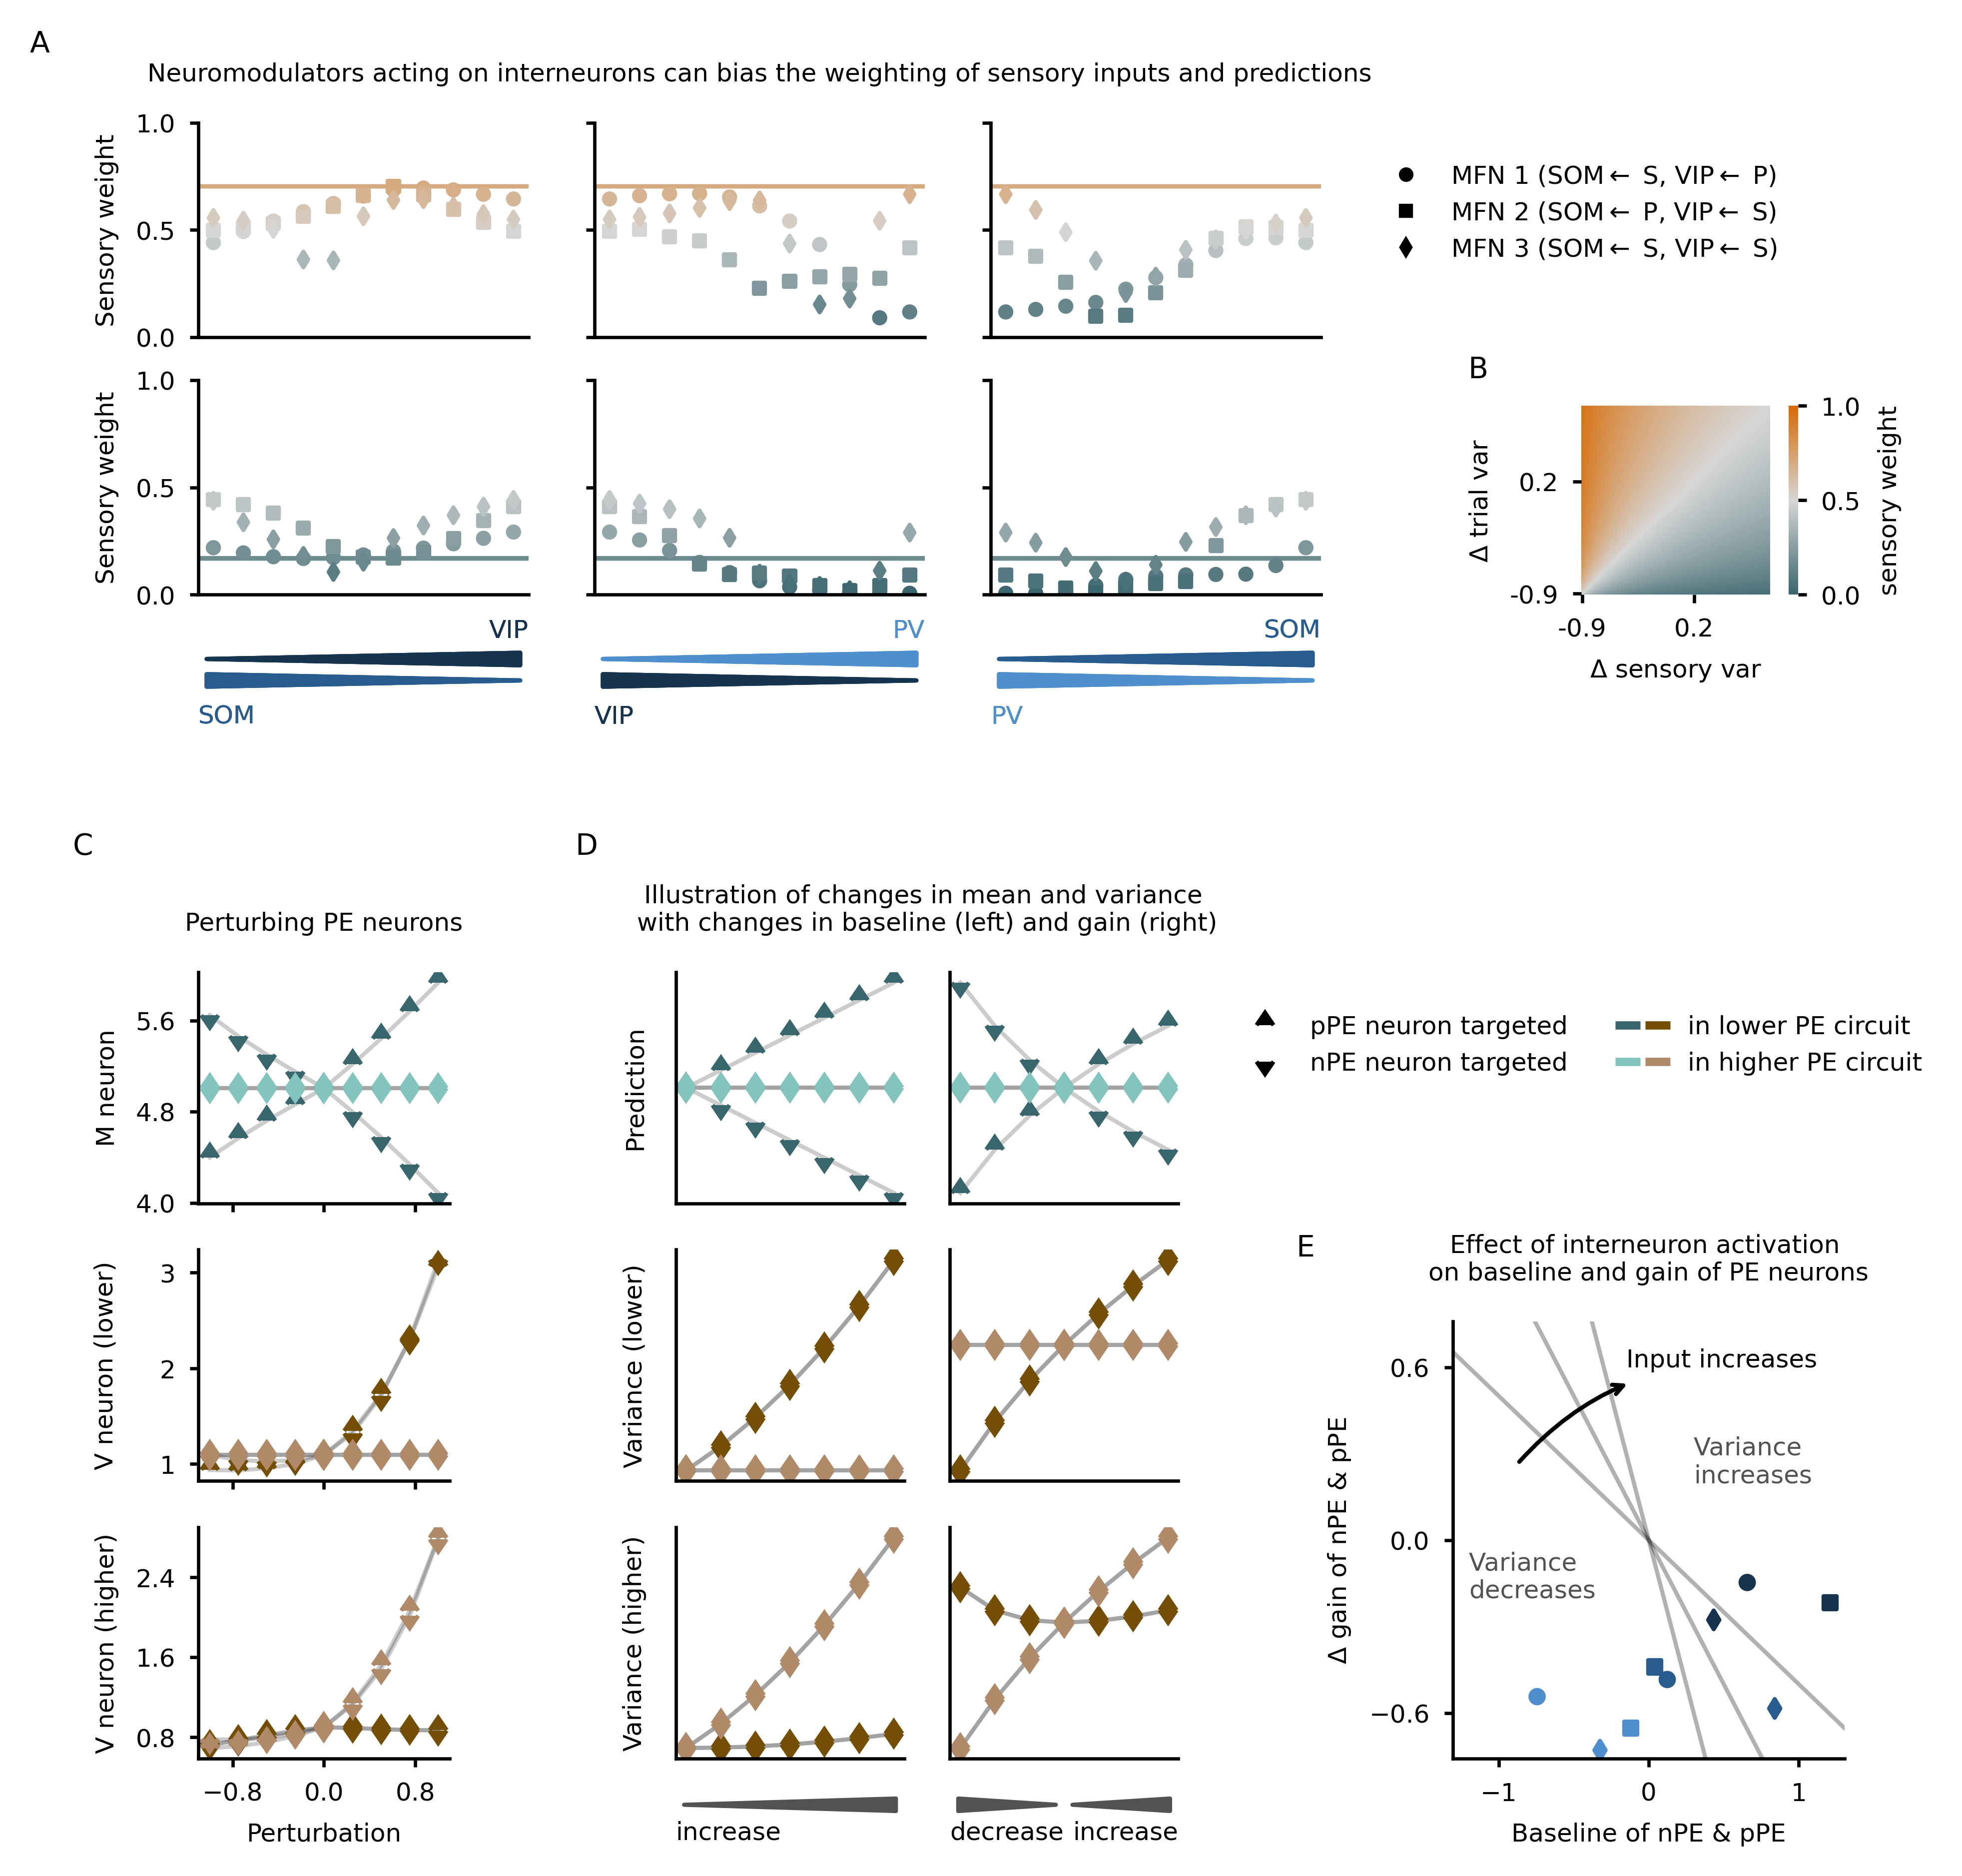
\includegraphics{../results/figures/final/Fig_4}%%%
\DIFdelendFL \DIFaddbeginFL 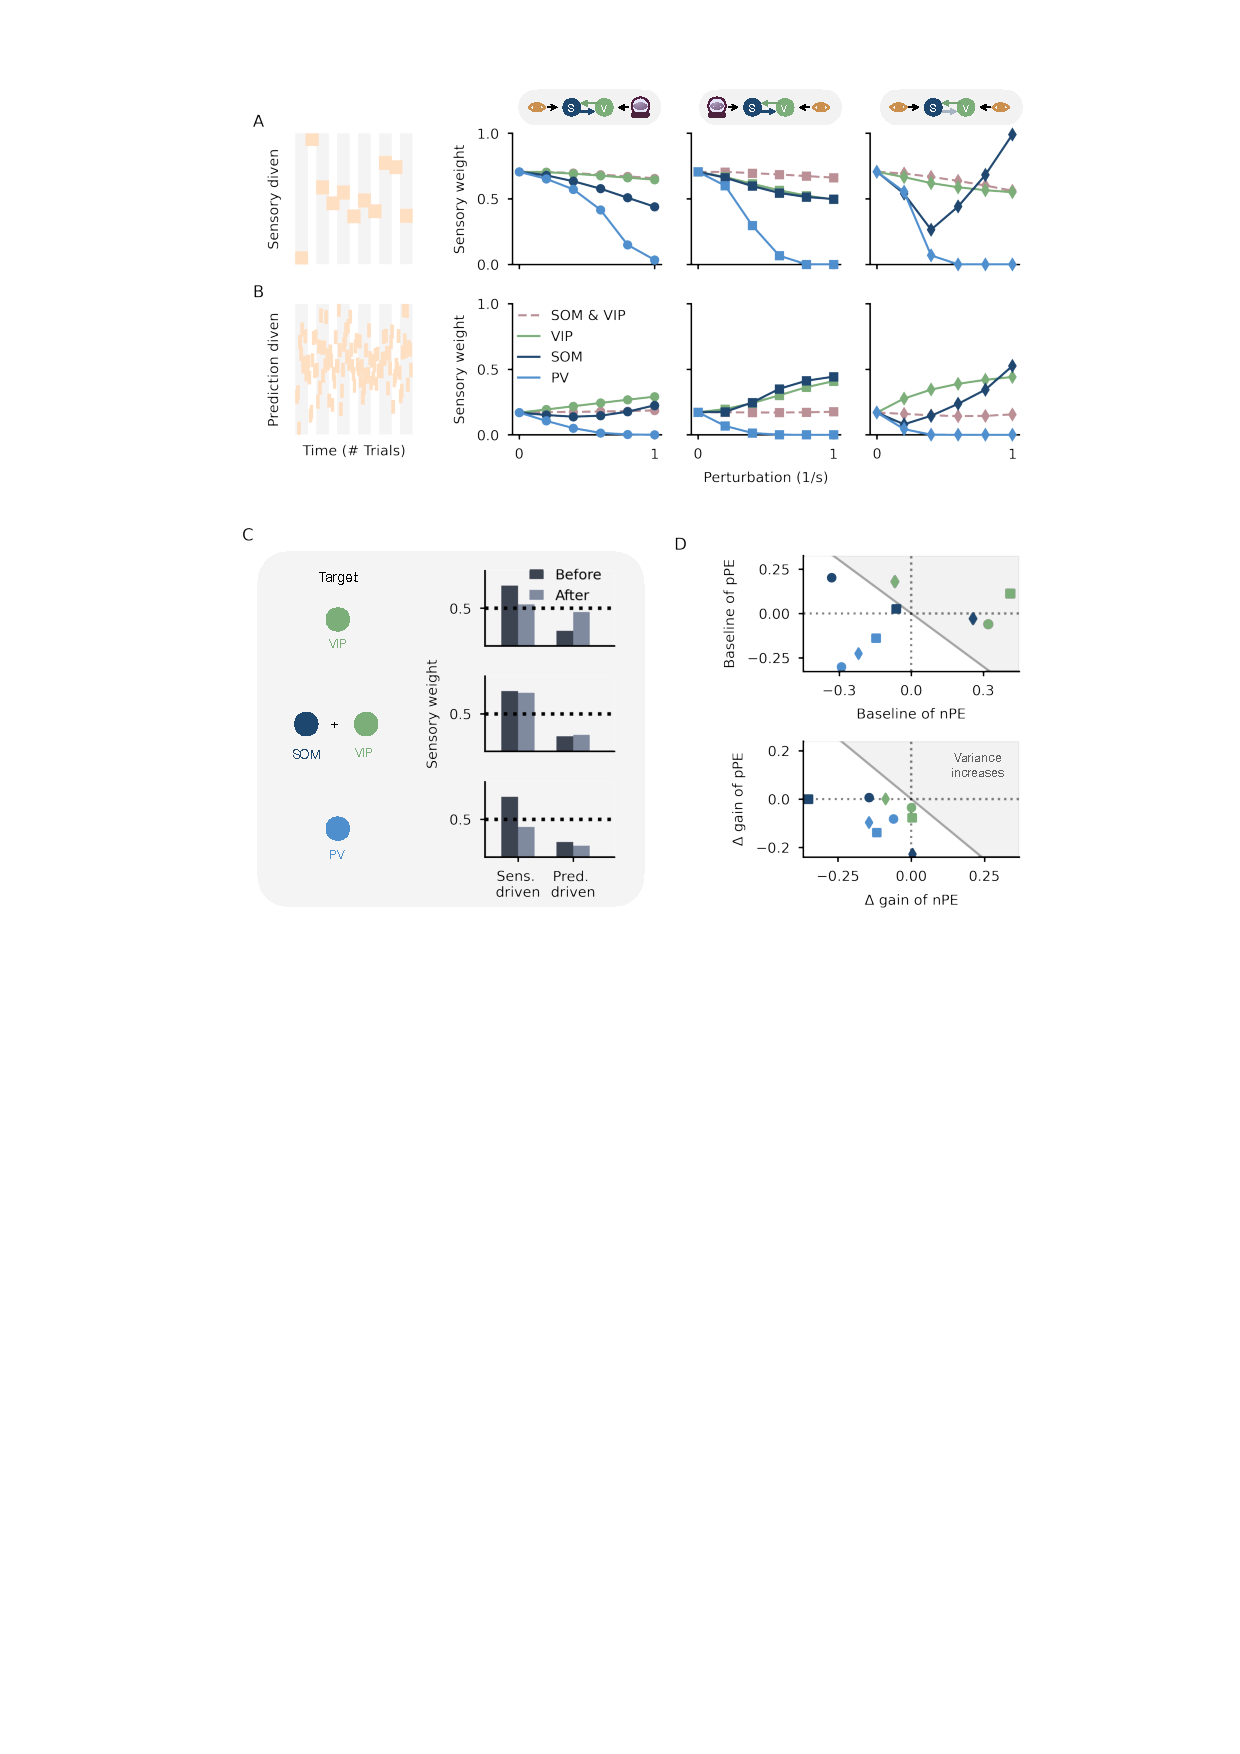
\includegraphics{../results/figures/final/Fig_4.pdf}\DIFaddendFL }
    %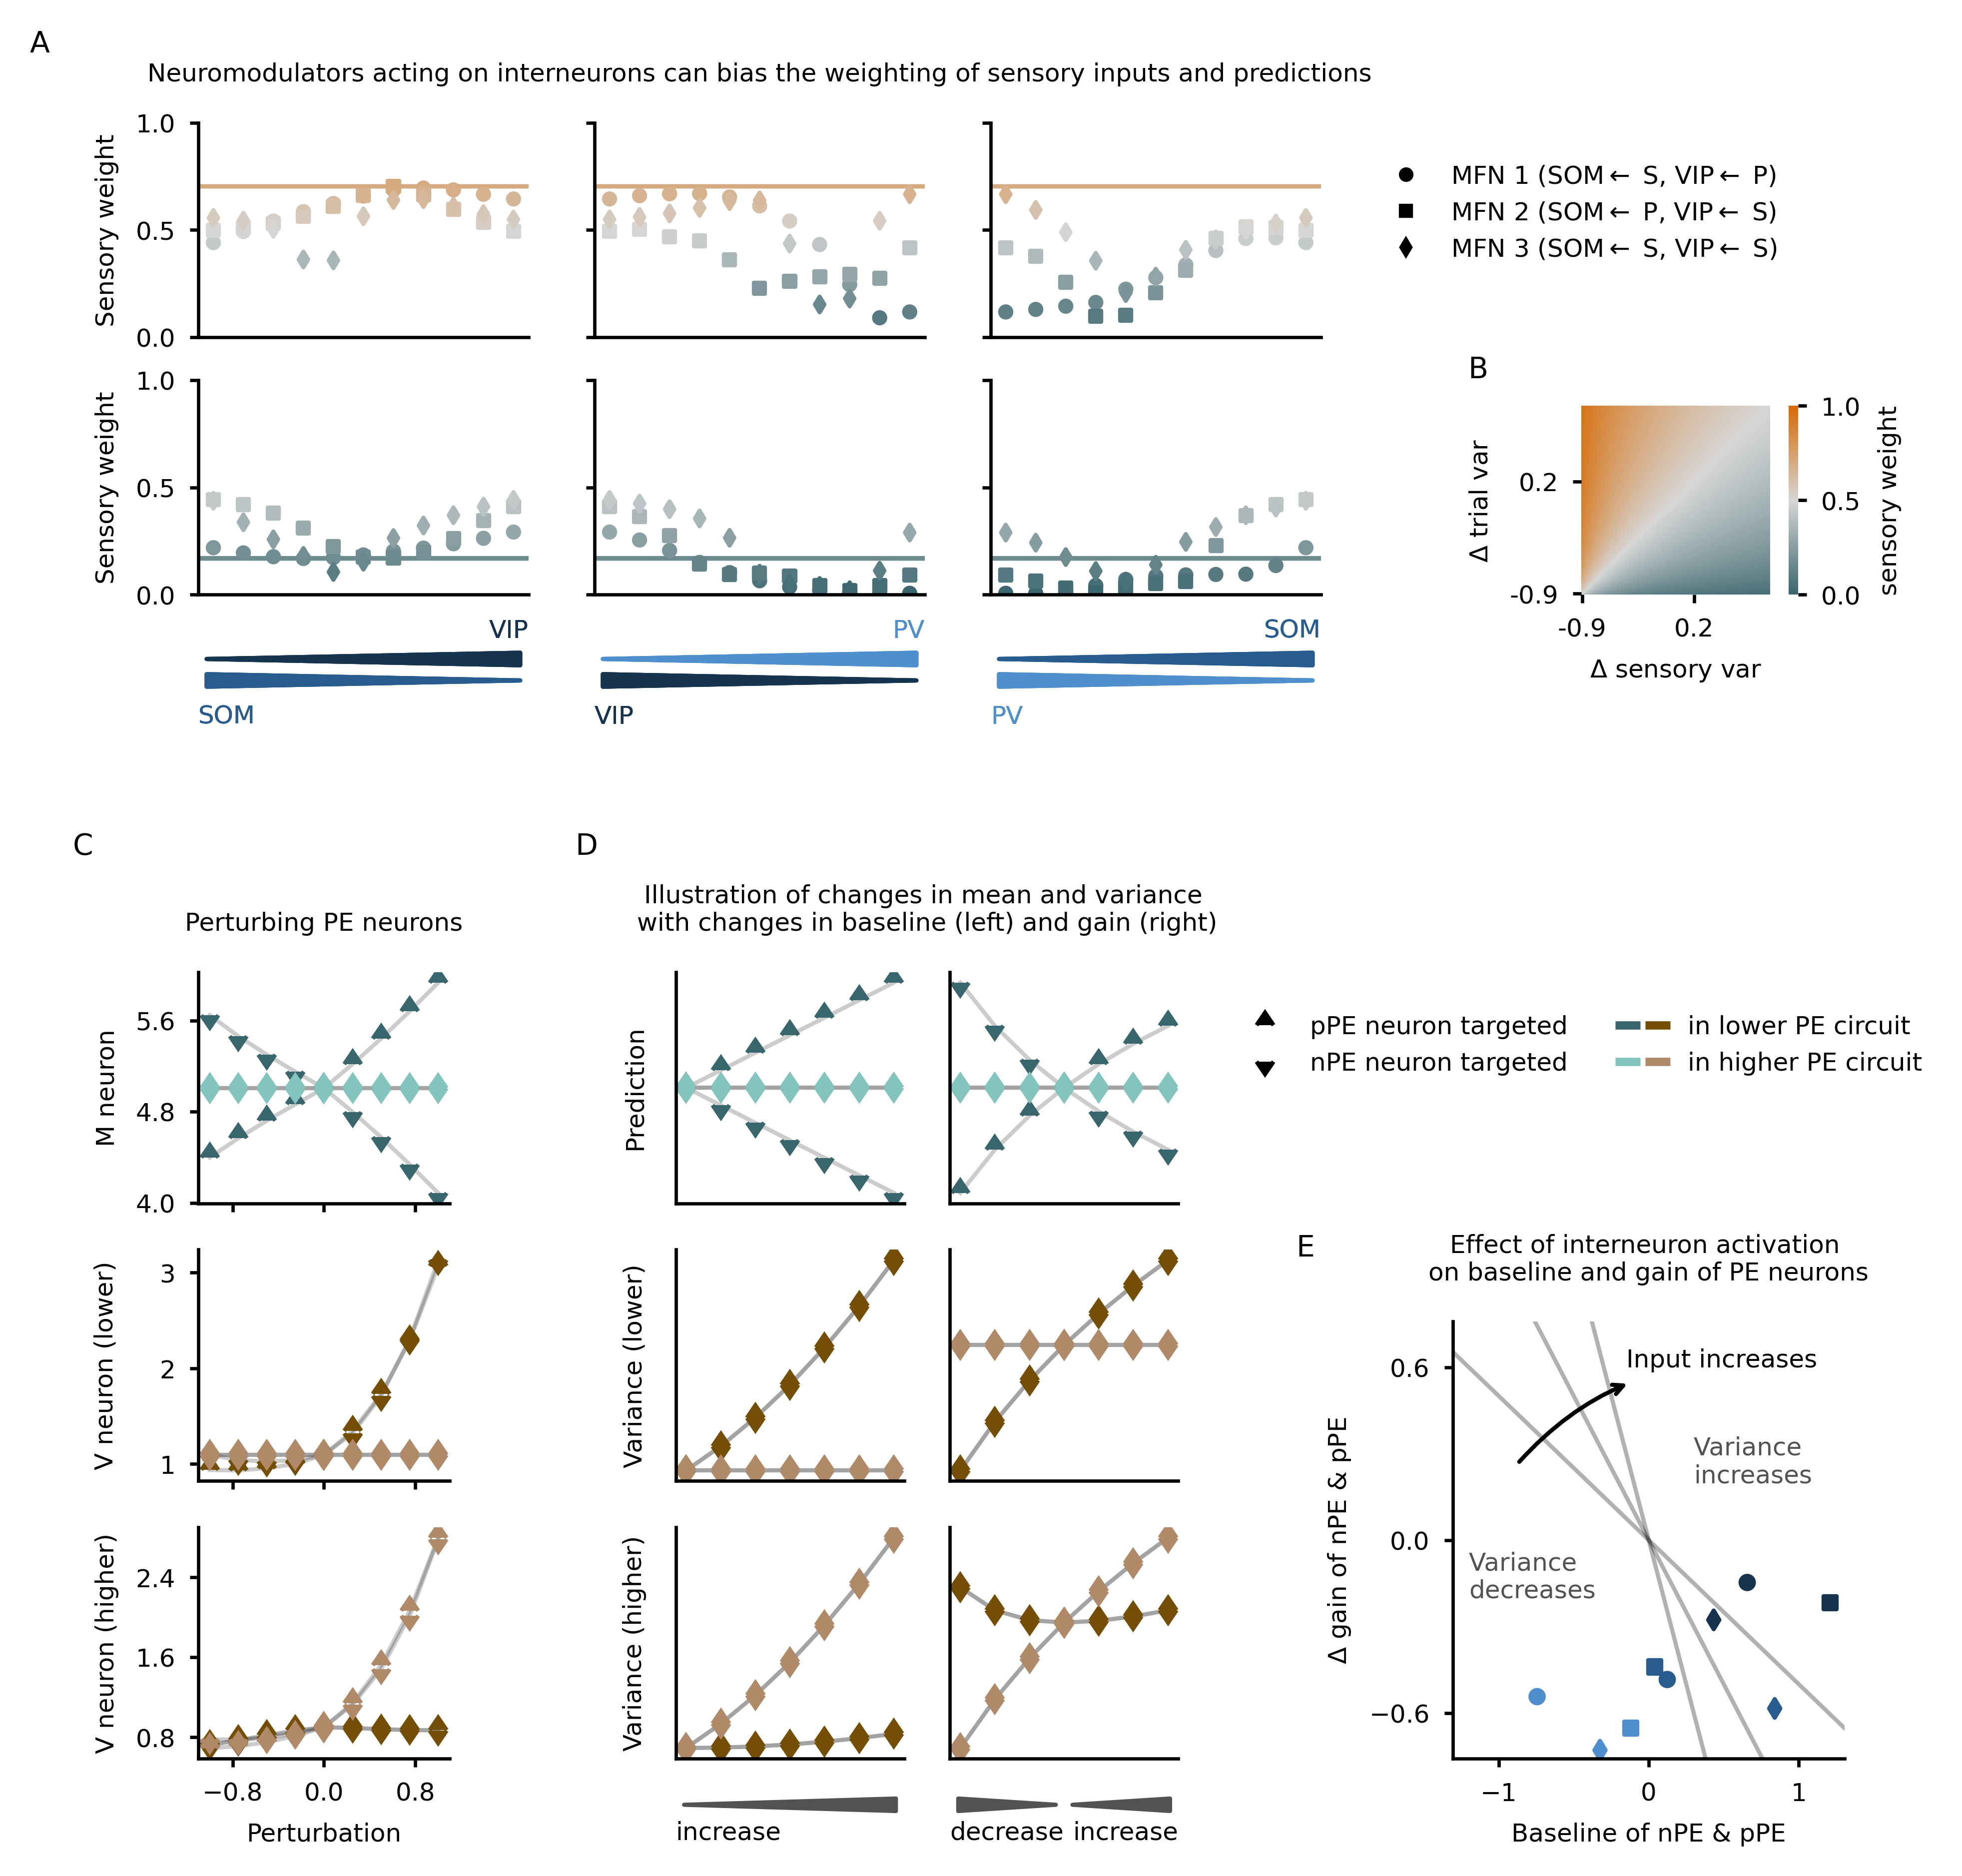
\includegraphics{../results/figures/final/Fig_4} % [width=1\linewidth]
\caption{\footnotesize{\bf Neuromodulator-based shifts in the weighting of sensory inputs and predictions.
\newline} 
{\bf (A)} Neuromodulators acting on the \DIFdelbeginFL \DIFdelFL{three }\DIFdelendFL interneurons \DIFdelbeginFL \DIFdelFL{may }\DIFdelendFL \DIFaddbeginFL \DIFaddFL{can }\DIFaddendFL shift the weighting of sensory inputs and predictions. The changes depend on the type \DIFdelbeginFL \DIFdelFL{/s }\DIFdelendFL of \DIFdelbeginFL \DIFdelFL{interneurons }\DIFdelendFL \DIFaddbeginFL \DIFaddFL{interneuron }\DIFaddendFL targeted \DIFdelbeginFL \DIFdelFL{by }\DIFdelendFL \DIFaddbeginFL \DIFaddFL{and }\DIFaddendFL the \DIFaddbeginFL \DIFaddFL{modulation strength (here simulated through an }\DIFaddendFL additional excitatory input\DIFdelbeginFL \DIFdelFL{emulating a neuromodulator (additional input = XXX}\DIFdelendFL ). Considered are two limit cases (upper row: more sensory-driven before modulation, lower row: more prediction-driven before modulation). The \DIFdelbeginFL \DIFdelFL{combination of interneurons targeted is illustrated below. The }\DIFdelendFL results are shown for three different PE circuits \DIFdelbeginFL \DIFdelFL{, specified in the main text}\DIFdelendFL \DIFaddbeginFL \DIFaddFL{(denotes by different markers)}\DIFaddendFL .
{\bf (B)} \DIFdelbeginFL \DIFdelFL{Illustration showing how }\DIFdelendFL \DIFaddbeginFL \DIFaddFL{When SOM and VIP neurons are equally modulated, }\DIFaddendFL the sensory weight \DIFdelbeginFL \DIFdelFL{depends on changes in both the stimulus and trial variability}\DIFdelendFL \DIFaddbeginFL \DIFaddFL{remains unaffected}\DIFaddendFL . 
{\bf (C)} The \DIFdelbeginFL \DIFdelFL{M and }\DIFdelendFL V \DIFdelbeginFL \DIFdelFL{neuron }\DIFdelendFL \DIFaddbeginFL \DIFaddFL{neurons' }\DIFaddendFL activities depend on the PE \DIFdelbeginFL \DIFdelFL{neuron activities}\DIFdelendFL \DIFaddbeginFL \DIFaddFL{neurons}\DIFaddendFL . Hence, perturbing the nPE and pPE neurons \DIFdelbeginFL \DIFdelFL{must change }\DIFdelendFL \DIFaddbeginFL \DIFaddFL{changes }\DIFaddendFL the \DIFaddbeginFL \DIFaddFL{uncertainty }\DIFaddendFL estimation\DIFdelbeginFL \DIFdelFL{of mean and variance}\DIFdelendFL . While stimulating the lower PE neurons affects both the lower and \DIFdelbeginFL \DIFdelFL{higher mean and variance estimation}\DIFdelendFL \DIFaddbeginFL \DIFaddFL{higher-order V neurons (right)}\DIFaddendFL , stimulating the \DIFdelbeginFL \DIFdelFL{higher }\DIFdelendFL \DIFaddbeginFL \DIFaddFL{higher-order }\DIFaddendFL PE neurons only affects the V \DIFdelbeginFL \DIFdelFL{and M neurons }\DIFdelendFL \DIFaddbeginFL \DIFaddFL{neuron }\DIFaddendFL in the same subnetwork \DIFaddbeginFL \DIFaddFL{(left)}\DIFaddendFL .
{\bf (D)} \DIFdelbeginFL \DIFdelFL{Illustration of }\DIFdelendFL \DIFaddbeginFL \DIFaddFL{The V neuron activity, and hence }\DIFaddendFL the \DIFdelbeginFL \DIFdelFL{mechanisms underlying the biased estimation }\DIFdelendFL \DIFaddbeginFL \DIFaddFL{sensory weight, changes as a result }\DIFaddendFL of \DIFdelbeginFL \DIFdelFL{mean and variance when }\DIFdelendFL \DIFaddbeginFL \DIFaddFL{the modulated }\DIFaddendFL PE \DIFdelbeginFL \DIFdelFL{neurons are perturbed}\DIFdelendFL \DIFaddbeginFL \DIFaddFL{neuron activity}\DIFaddendFL . \DIFdelbeginFL \DIFdelFL{Both }\DIFdelendFL \DIFaddbeginFL \DIFaddFL{The PE neuron activity, on the other hand, }\DIFaddendFL changes \DIFdelbeginFL \DIFdelFL{in }\DIFdelendFL \DIFaddbeginFL \DIFaddFL{as a result of }\DIFaddendFL the \DIFaddbeginFL \DIFaddFL{interneurons being modulated. The interneurons change the }\DIFaddendFL baseline (left) and \DIFaddbeginFL \DIFaddFL{the }\DIFaddendFL gain (right) of \DIFdelbeginFL \DIFdelFL{PE neurons can contribute to }\DIFdelendFL the \DIFdelbeginFL \DIFdelFL{changes observed in (C). Illustration based on toy model described in Methods.
}%DIFDELCMD < {\bf %%%
\DIFdelFL{(E)}%DIFDELCMD < } %%%
\DIFdelFL{Modulated interneurons change the weighting by changing the overall baseline and the overall gain of }\DIFdelendFL PE neurons\DIFdelbeginFL \DIFdelFL{(sum of changes in nPE and pPE neurons)}\DIFdelendFL . Whether \DIFdelbeginFL \DIFdelFL{and how a neuromodulator changes }\DIFdelendFL \DIFaddbeginFL \DIFaddFL{an interneuron increases or decreases }\DIFaddendFL the \DIFdelbeginFL \DIFdelFL{sensory weight, hence, }\DIFdelendFL \DIFaddbeginFL \DIFaddFL{estimated variance }\DIFaddendFL depends on \DIFdelbeginFL \DIFdelFL{the interneuron targeted and the effect this interneuron has on baseline and gain of the PE neurons, which in turn does depend on the network it is embedded in}\DIFdelendFL \DIFaddbeginFL \DIFaddFL{both factors}\DIFaddendFL .
}
\label{fig:Fig_4}
\end{figure}
%

To this end, we modeled the presence of \DIFdelbegin \DIFdel{neuromodulators }\DIFdelend \DIFaddbegin \DIFadd{a neuromodulator }\DIFaddend by injecting an additional excitatory input into \DIFdelbegin \DIFdel{one or two interneuron types}\DIFdelend \DIFaddbegin \DIFadd{an interneuron type}\DIFaddend . We reasoned that the network effect of a neuromodulator not only depends on the interneuron type it targets but also on the inputs this neuron receives and the connections it makes with other neurons in the network. We, therefore, tested \DIFdelbegin \DIFdel{three }\DIFdelend different mean-field networks that differ \DIFdelbegin \DIFdel{with respect to }\DIFdelend \DIFaddbegin \DIFadd{in }\DIFaddend the distribution of sensory inputs and predictions onto the interneurons, and the underlying connectivity. The commonality across those networks is that they exhibit an E/I balance of excitatory and inhibitory pathways onto the PE neurons \DIFdelbegin \DIFdel{(XXX). 
}\DIFdelend \DIFaddbegin \DIFadd{\mbox{%DIFAUXCMD
\citep{hertag2022prediction}}\hskip0pt%DIFAUXCMD
. 
}

\DIFaddend Across the different mean-field networks tested, \DIFdelbegin \DIFdel{activating a SOM or VIP neuron individually }\DIFdelend \DIFaddbegin \DIFadd{increasing the activity of PV neurons biases the network's output toward predictions (Fig. \ref{fig:Fig_4}A left). In contrast, increasing VIP activity }\DIFaddend forces the networks to weigh both inputs more equally. As a consequence, predictions are overrated in a sensory-driven input regime\DIFdelbegin \DIFdel{. Similarly, }\DIFdelend \DIFaddbegin \DIFadd{, and, }\DIFaddend sensory inputs are overrated in a prediction-driven input regime \DIFdelbegin \DIFdel{. Interestingly, when both interneuron types are activated to the same degree, this effect disappears }\DIFdelend (Fig. \ref{fig:Fig_4}A \DIFdelbegin \DIFdel{, left). In contrast, stimulating PV neurons biases the network's output towards predictions. This effect is even more pronounced when PV and SOM, or PV and VIP neurons are activated simultaneously }\DIFdelend \DIFaddbegin \DIFadd{right). Increasing SOM neuron activity, while qualitatively similar to increasing VIP neuron activity, depends on the mean-field network tested and the strength of activation }\DIFaddend (Fig. \ref{fig:Fig_4}A \DIFdelbegin \DIFdel{, middleand right}\DIFdelend \DIFaddbegin \DIFadd{middle}\DIFaddend ). 

\DIFdelbegin \DIFdel{In the previous simulations, we assumed that a neuromodulator acts globally, that is, on the interneurons in both the lower and the higher PE circuit. While this agrees with experimental data showing that XXX (XXX), we note that neuromodulators may also act more locally. The effect of stimulating an interneuron type in the lower PE circuit on the sensory weight is mostly the opposite of activating the same interneuron in the higher PE circuit }\DIFdelend \DIFaddbegin \DIFadd{Neuromodulators are most likely increasing the activity of more than one interneuron type. To account for the co-activation of interneurons, we injected an excitatory input into two interneuron types at the same time and varied the strength with which each interneuron was modulated }\DIFaddend (Fig. \ref{fig:Fig_4_S1}). \DIFdelbegin \DIFdel{For instance, the sensory inputs are overrated when the higher-level VIP neuron is activated, while the prediction is overrated when the lower-level VIP neuron is activated. When VIP and SOM neurons are stimulated equally , }\DIFdelend \DIFaddbegin \DIFadd{If PV neurons are }\DIFaddend the \DIFdelbegin \DIFdel{sensory weight remains unchanged, independently of which PE circuit is targeted by the neuromodulator}\DIFdelend \DIFaddbegin \DIFadd{major target of a neuromodulator, the network is still biased toward predictions. If SOM and VIP neurons are equally stimulated, the weighting of sensory inputs and predictions remains largely unaffected (Fig. \ref{fig:Fig_4}B), suggesting that the individual effects cancel out}\DIFaddend .

What are the \DIFdelbegin \DIFdel{mechanisms that give rise to these effects? And how do the combined local changes give rise to the global one observed in our network simulations? }\DIFdelend \DIFaddbegin \DIFadd{network mechanisms underlying these observation? }\DIFaddend The sensory weight is \DIFdelbegin \DIFdel{chosen to be }\DIFdelend a function of the \DIFdelbegin \DIFdel{V neurons of the }\DIFdelend lower and higher \DIFdelbegin \DIFdel{PE circuit}\DIFdelend \DIFaddbegin \DIFadd{V neuron activity}\DIFaddend . Hence, any changes to the sensory weight result from changes to the neurons encoding the variances\DIFdelbegin \DIFdel{(Fig. \ref{fig:Fig_4}B). }\DIFdelend \DIFaddbegin \DIFadd{. }\DIFaddend In our network, the V neurons only receive excitatory \DIFdelbegin \DIFdel{output }\DIFdelend synapses from PE neurons. Hence, any changes in the sensory weights upon activation of interneurons must be due to changes in the PE neurons. To disentangle the effect of nPE and pPE neurons, we perturbed those neurons individually in both the lower or higher subnetwork by injecting either an inhibitory or excitatory additional input (Fig. \ref{fig:Fig_4}C).
Stimulating either PE neuron in the lower subnetwork increases the activity of the lower-level V neuron strongly. Moreover, the higher-level V neuron is also slightly affected. \DIFdelbegin \DIFdel{At first, this is counterintuitive because the V neuron in the higher subnetwork does not receive direct synapses from the PE neurons in the lower subnetwork. However, the activity of the }\DIFdelend \DIFaddbegin \DIFadd{This is because the }\DIFaddend lower-level M neuron \DIFdelbegin \DIFdel{encoding the prediction increases with an excitatory input onto the pPE neuron and decreases with an excitatory input onto the nPE neuron (the opposite is true for an inhibitory input). Because neurons in the higher PE circuit receive synapses from the lower-level M neuron, the activity of the }\DIFdelend \DIFaddbegin \DIFadd{is also modulated by the lower-level PE neurons and makes feedforward connections to the }\DIFaddend higher-level \DIFdelbegin \DIFdel{V neuron is also affected}\DIFdelend \DIFaddbegin \DIFadd{PE circuit}\DIFaddend . In contrast, stimulating either PE neuron in the higher subnetwork increases the activity of the higher-level V neuron but leaves the lower-level \DIFdelbegin \DIFdel{M and V neurons unaffected(Fig. 
\ref{fig:Fig_4}C).
}\DIFdelend \DIFaddbegin \DIFadd{neurons unaffected. 
}\DIFaddend 

\DIFdelbegin \DIFdel{Stimulating PE neurons may cause both an increase in the baseline activity and a change in the neuron's gain. To disentangle both effects, we illustrate each contribution separately using a mathematically tractable toy model (see Methods for more details). The variance estimated in the lower subnetwork increases with both increasing baseline and gain of the lower-level PE neurons. In contrast, when the gain of those PE neurons decreases, so does the variance. Similarly, the variance estimated in the higher subnetwork is equally influenced by changes in baseline and gain of the higher-level PE neurons. Moreover, changes to the baseline and the gain of the lower-level PE neurons increases the higher-level variance as a result of a biased prediction. Furthermore, the mean of the sensory stimuli is overpredicted (underpredicted) when the baseline or the gain of the lower-level pPE (nPE) neuron increases, or when the gain of the lower-level nPE (pPE) neuron decreases. In summary, if an interneuron causes an additional inhibitory input to a PE neuron, the neuron's gain is reduced. If an interneuron causes an additional disinhibitory input to a PE neuron, the neuron's baseline and gain are increased (Fig. \ref{fig:Fig_4}D).
}%DIFDELCMD < 

%DIFDELCMD < %%%
\DIFdelend This suggests that to understand the effect of neuromodulators on the sensory weight, we need to unravel the effect of interneuron activation on \DIFdelbegin \DIFdel{baseline and gain of }\DIFdelend PE neurons. \DIFdelbegin \DIFdel{To this end, we stimulated either PV, SOM, or VIP neurons independently for all three mean-field networks and measured the changes to }\DIFdelend \DIFaddbegin \DIFadd{Increasing interneuron activity leads to changes in the }\DIFaddend baseline and gain of \DIFdelbegin \DIFdel{both PE neurons }\DIFdelend \DIFaddbegin \DIFadd{PE neurons that bias the estimation of mean and variance }\DIFaddend (Fig. \DIFdelbegin \DIFdel{\ref{fig:Fig_4}E}\DIFdelend \DIFaddbegin \DIFadd{\ref{fig:Fig_4_S3}, see Methods}\DIFaddend ). In all three networks tested, activating PV neurons decreases both \DIFdelbegin \DIFdel{quantities}\DIFdelend \DIFaddbegin \DIFadd{baseline and gain of the PE neurons}\DIFaddend , leading to a decrease in the estimated variance (Fig. \ref{fig:Fig_4}\DIFdelbegin \DIFdel{E }\DIFdelend \DIFaddbegin \DIFadd{D }\DIFaddend \& Fig. \DIFdelbegin \DIFdel{\ref{fig:Fig_4_S2}}\DIFdelend \DIFaddbegin \DIFadd{\ref{fig:Fig_4_S4}}\DIFaddend ). Stimulating \DIFaddbegin \DIFadd{the }\DIFaddend SOM or VIP \DIFdelbegin \DIFdel{neurons decreases the overall gain but increases the baseline activity of the PE neurons . Whether and how much the gain of the nPE or pPE neuron is reduced depends on the inputs onto SOM and VIP neurons, and the connectivity they make }\DIFdelend \DIFaddbegin \DIFadd{neuron decreases the gain in either nPE or pPE neuron. However, the baseline of those neurons can either decrease or increase depending on the connectivity }\DIFaddend with other neurons in the network. \DIFdelbegin \DIFdel{Similarly, how much the baseline is elevated depends on the specifics of the mean-field network }\DIFdelend \DIFaddbegin \DIFadd{The summed effect over nPE and pPE neuron }\DIFaddend (Fig. \DIFdelbegin \DIFdel{\ref{fig:Fig_4}E \& Fig. \ref{fig:Fig_4_S2}). Hence, whether stimulating the SOM or VIP neuron decreases or increases the }\DIFdelend \DIFaddbegin \DIFadd{\ref{fig:Fig_4_S4}), hence, suggests that whether the }\DIFaddend activity of the V neuron \DIFaddbegin \DIFadd{increases or decreases }\DIFaddend depends on the input statistics: for low-mean stimuli, the elevated baseline activity dominates the changes in the variance, while for high-mean stimuli the changes in the gain dominate.

%DIF < XXX Summary ... effect of neuromodulators acting on INs on sensory weight best understood as combined effect on the baseline and gain of nPE and pPE neurons that in turn determine the activity of the V neuron. Those effects not ony depend on the target IN but also the network in which it is embedded, that is the connectivity and the inputs onto INs. Moreover, it depends on whether local or global. The effects of activation on lower is mainly the opposite of same in higher. However, the efefcts don't cancel each other in global modulation. Mostly because 1) V higher additionally changes due to changes in prediction but also 2) effects in higher are stronger !? and 3) 1/(1+(Vs + D)/(Vp + D)) ... that is it cannot cancel per se. Even though the underlying reasons for a change in the V neuron depends on the the network characteristics, there are some consistent changes in sensory weigt across MFN ... name
\DIFaddbegin \DIFadd{Altogether, we show that neuromodulators increasing the activity of interneurons bias the weighting of sensory inputs and predictions by changing the gain and baseline of PE neurons. Whether the sensory weight increases or decreases depends not only on the interneuron it targets but also on the network it is embedded in and the input regime.
}\DIFaddend 


%DIF <  in caption: you need to make sure that in e you used a perturbation of 1 and the mean and std of stimuli were ... the lines only illustrate that it depends on the input statistics. Of course, the markers would also change with other perturbaton strengths, would they though? Think through
%DIF <  Mention that for V neuron (higher) the darker line is actually not horizontal (unaffected)!
%DIF <  Mention that in BL illustration you need a factor to increase visibility ... (in caption)
\DIFdelbegin %DIFDELCMD < 

%DIFDELCMD < %%%
\DIFdelend \subsection*{\DIFdelbegin \DIFdel{The }\DIFdelend \DIFaddbegin \DIFadd{Explaining the }\DIFaddend contraction bias \DIFdelbegin \DIFdel{as a result of }\DIFdelend \DIFaddbegin \DIFadd{with }\DIFaddend the \DIFdelbegin \DIFdel{weighted integration }\DIFdelend \DIFaddbegin \DIFadd{weighting }\DIFaddend of sensory inputs and predictions}
% 
\DIFdelbegin \DIFdel{The }\DIFdelend \DIFaddbegin \DIFadd{We hypothesized that the }\DIFaddend weighted integration of sensory inputs and predictions thereof manifests in all-day behavior, in the form of a phenomenon called \textit{contraction bias}. The contraction bias describes the tendency to overestimate sensory stimuli drawn from the lower end of a stimulus distribution and to underestimate stimuli drawn from the upper end of the same distribution\DIFdelbegin \DIFdel{(Fig. \ref{fig:Fig_5}A). This }\DIFdelend \DIFaddbegin \DIFadd{. This }\DIFaddend \textit{bias \DIFdelbegin \DIFdel{towards }\DIFdelend \DIFaddbegin \DIFadd{toward }\DIFaddend the mean} has been reported in different species and modalities \DIFdelbegin \DIFdel{(XXX)}\DIFdelend \DIFaddbegin \DIFadd{\mbox{%DIFAUXCMD
\citep{hollingworth1910central, jazayeri2010temporal, ashourian2011bayesian, petzschner2011iterative, akrami2018posterior, meirhaeghe2021precise}}\hskip0pt%DIFAUXCMD
}\DIFaddend . 
%
\begin{figure}[t!]
	\centering
    \DIFdelbeginFL %DIFDELCMD < 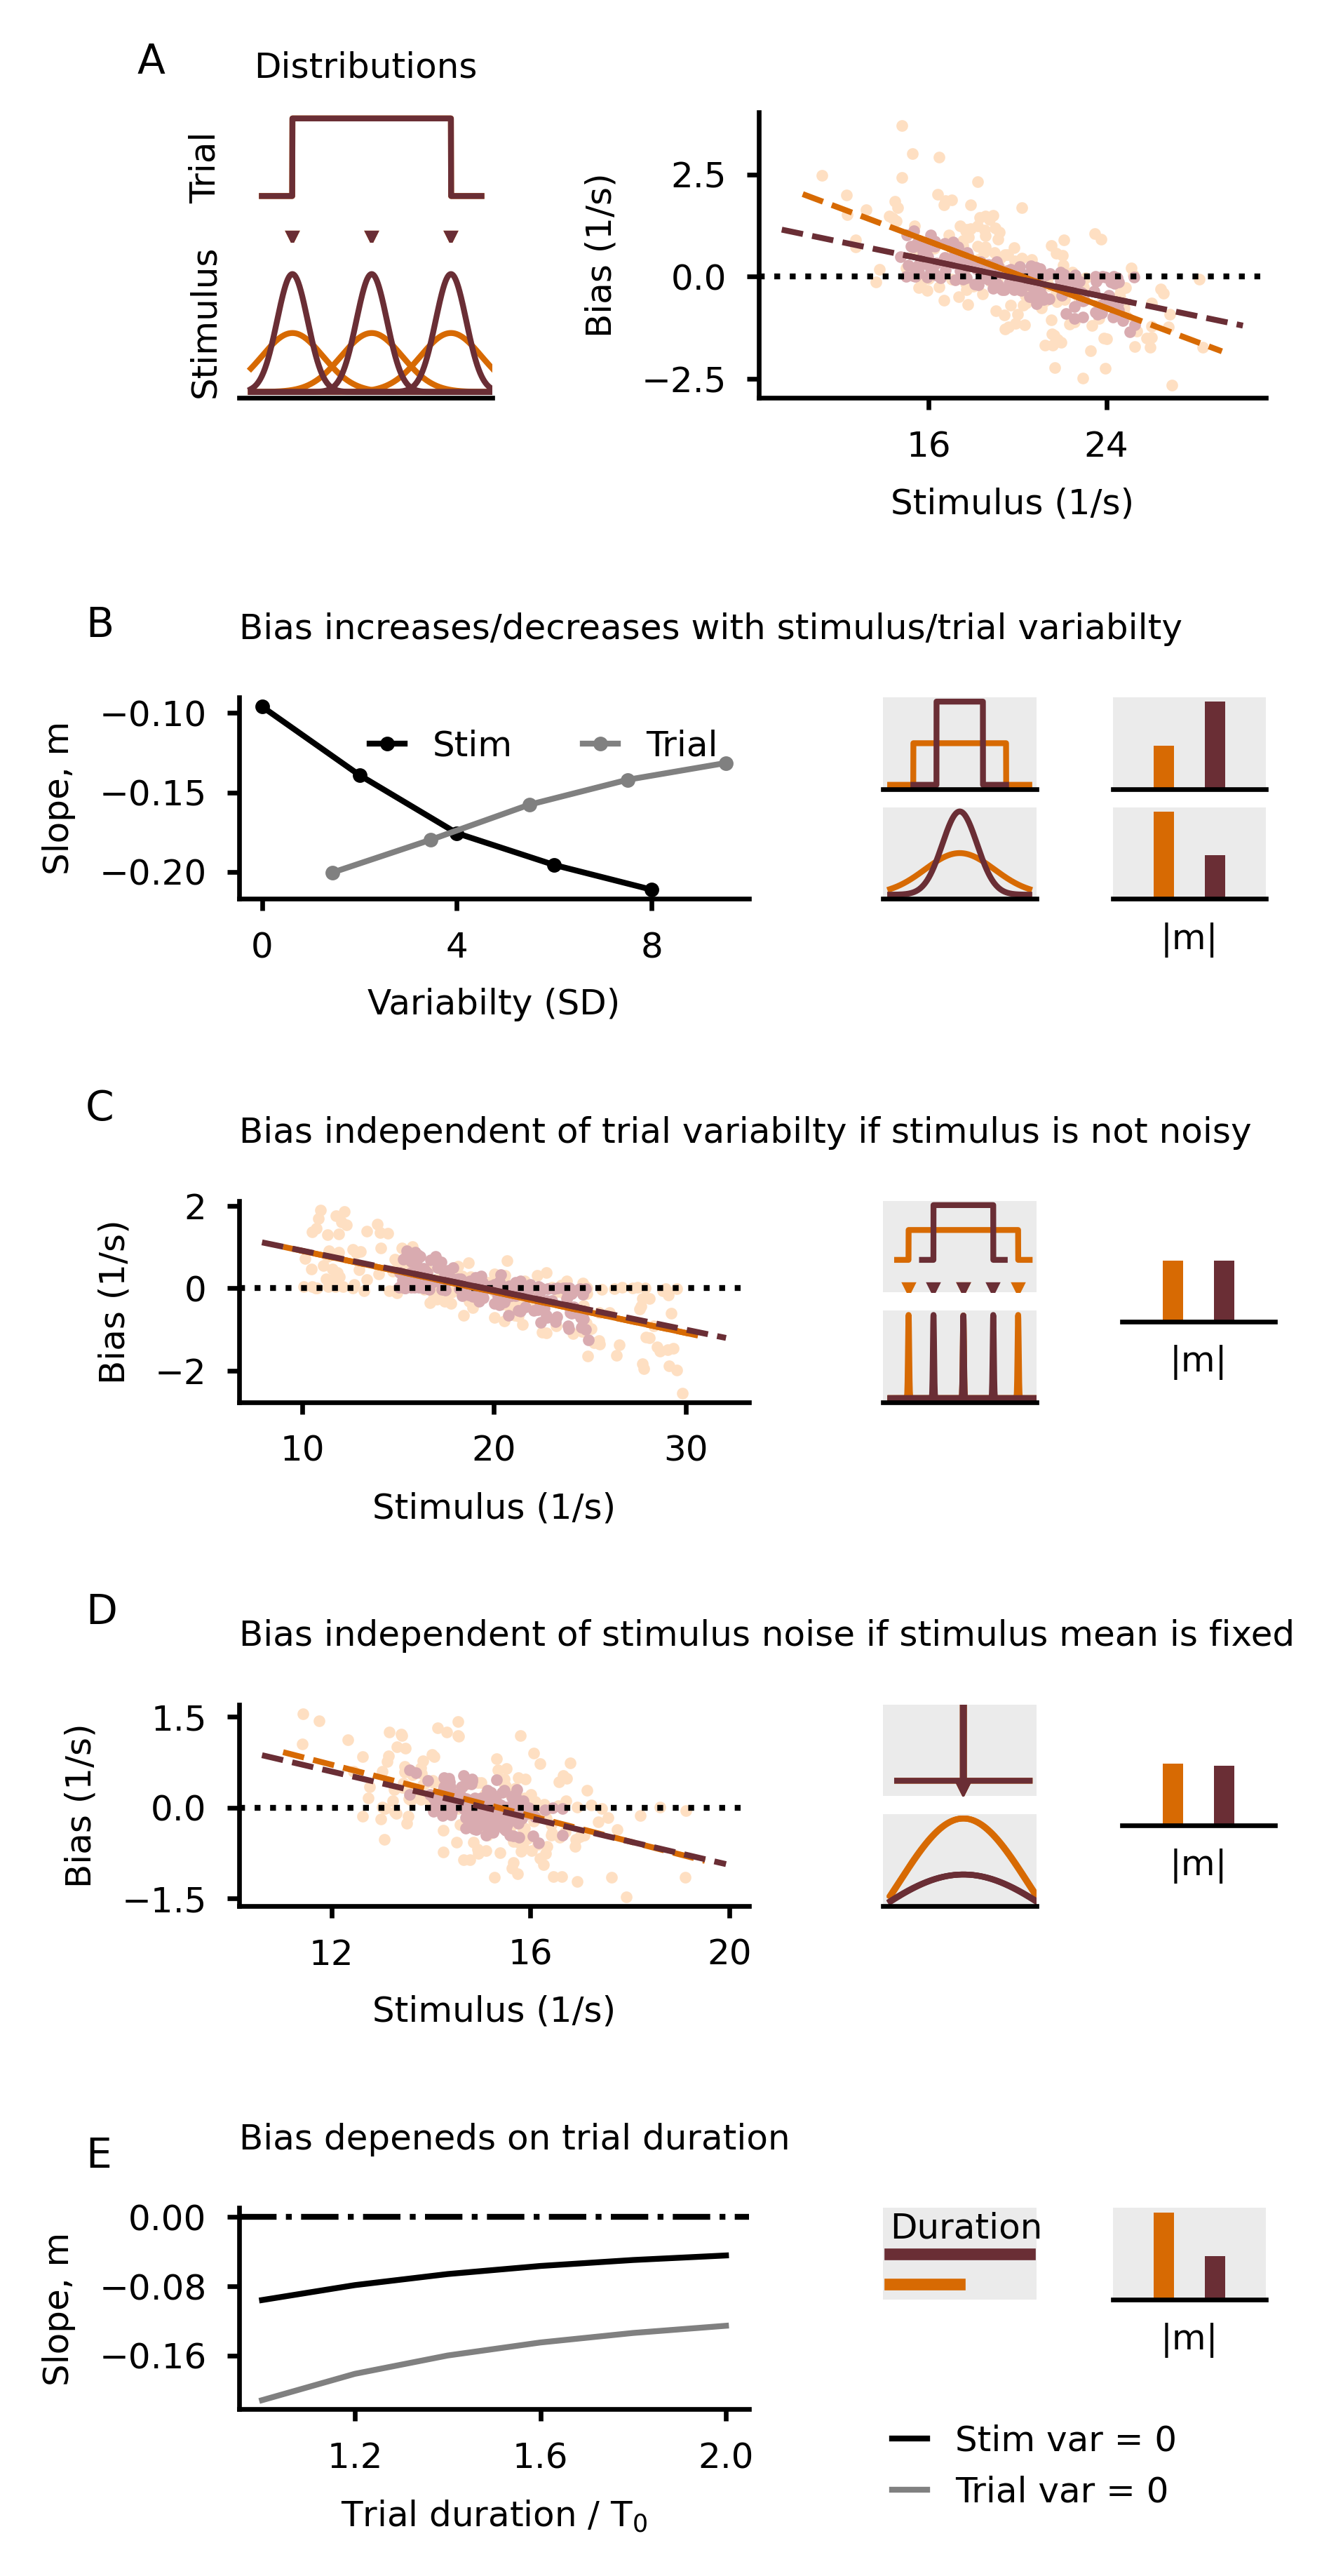
\includegraphics{../results/figures/final/Fig_5}
%DIFDELCMD < %%%
\DIFdelendFL \DIFaddbeginFL 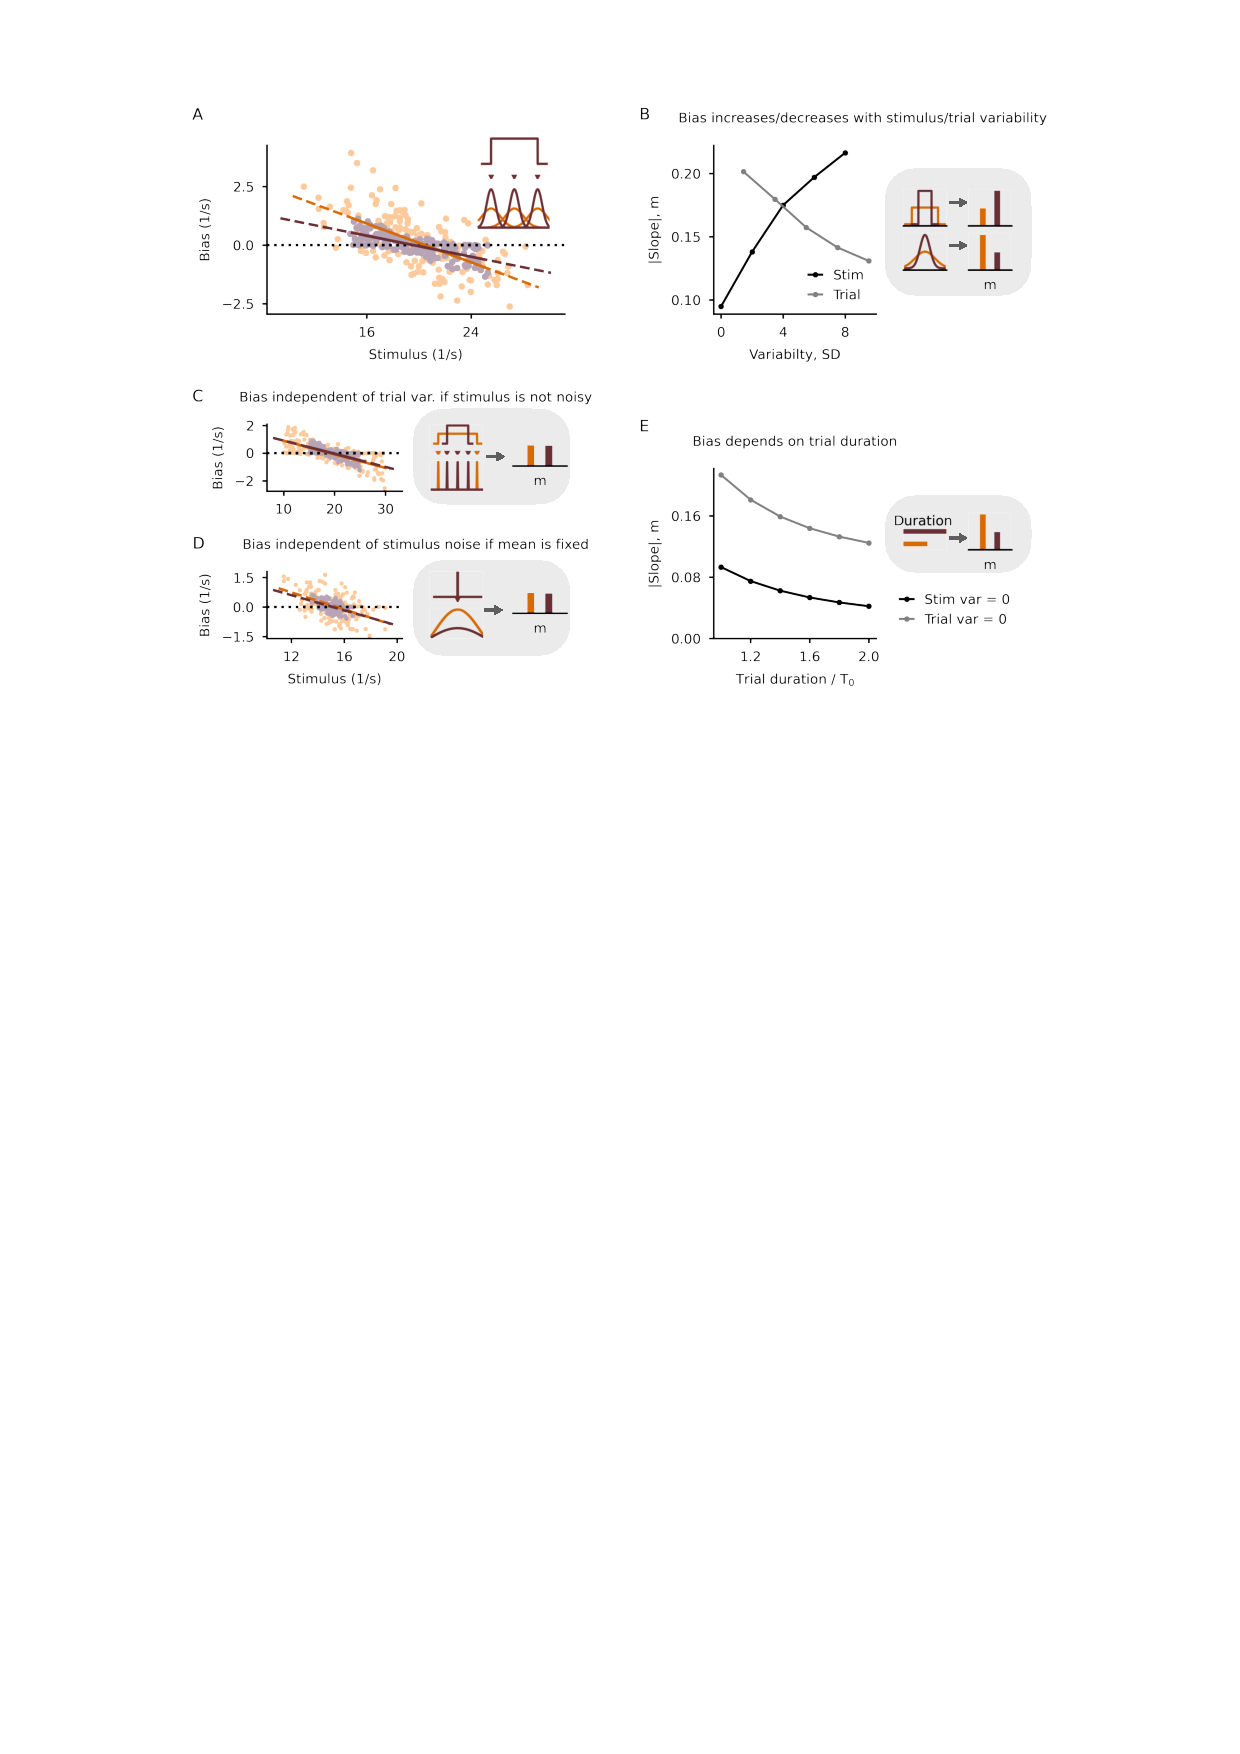
\includegraphics{../results/figures/final/Fig_5.pdf}
\DIFaddendFL \caption{\footnotesize{\bf Mechanisms underlying the contraction bias.\newline} 
{\bf (A)} \DIFdelbeginFL \DIFdelFL{Illustration of the contraction }\DIFdelendFL \DIFaddbeginFL \DIFaddFL{Contraction }\DIFaddendFL bias \DIFaddbeginFL \DIFaddFL{in the model for two different stimulus uncertainties depicted in the inset}\DIFaddendFL . \DIFdelbeginFL \DIFdelFL{The estimated input }\DIFdelendFL \DIFaddbeginFL \DIFaddFL{Bias }\DIFaddendFL is \DIFdelbeginFL \DIFdelFL{shifted towards }\DIFdelendFL \DIFaddbeginFL \DIFaddFL{defined as }\DIFaddendFL the \DIFaddbeginFL \DIFaddFL{weighted output minus the stimulus }\DIFaddendFL mean\DIFaddbeginFL \DIFaddFL{. The absolute value }\DIFaddendFL of the \DIFdelbeginFL \DIFdelFL{input distribution. Hence, a linear curve fitted to the data has a }\DIFdelendFL slope \DIFdelbeginFL \DIFdelFL{below 1 }\DIFdelendFL (\DIFdelbeginFL \DIFdelFL{left}\DIFdelendFL \DIFaddbeginFL \DIFaddFL{see linear fit}\DIFaddendFL ) \DIFaddbeginFL \DIFaddFL{is a measure of the bias}\DIFaddendFL . The \DIFdelbeginFL \DIFdelFL{bias is biggest at }\DIFdelendFL \DIFaddbeginFL \DIFaddFL{larger }\DIFaddendFL the \DIFdelbeginFL \DIFdelFL{end of }\DIFdelendFL \DIFaddbeginFL \DIFaddFL{slope, }\DIFaddendFL the \DIFdelbeginFL \DIFdelFL{stimulus distribution (right)}\DIFdelendFL \DIFaddbeginFL \DIFaddFL{larger the bias}\DIFaddendFL .
{\bf (B)}  \DIFdelbeginFL \DIFdelFL{Contraction bias in the model. Left: Example for two different stimulus variabilities. Right: }\DIFdelendFL As a consequence of the sensory weight, the slope \DIFdelbeginFL \DIFdelFL{decreases }\DIFdelendFL \DIFaddbeginFL \DIFaddFL{increases }\DIFaddendFL with stimulus variability (bias increases) and \DIFdelbeginFL \DIFdelFL{increases }\DIFdelendFL \DIFaddbeginFL \DIFaddFL{decreases }\DIFaddendFL with trial variability (bias decreases).
\DIFdelbeginFL \DIFdelFL{Stimulus statistics: XXX.
}\DIFdelendFL {\bf (C)} \DIFdelbeginFL \DIFdelFL{The bias }\DIFdelendFL \DIFaddbeginFL \DIFaddFL{Bias }\DIFaddendFL is independent of \DIFaddbeginFL \DIFaddFL{the }\DIFaddendFL trial variability when the stimulus variability is zero\DIFaddbeginFL \DIFaddFL{.
}{\bf \DIFaddendFL (\DIFdelbeginFL \DIFdelFL{left}\DIFdelendFL \DIFaddbeginFL \DIFaddFL{D}\DIFaddendFL )\DIFdelbeginFL \DIFdelFL{. Equally, the bias }\DIFdelendFL \DIFaddbeginFL } \DIFaddFL{Bias }\DIFaddendFL is independent of the stimulus variability when the trial variability is zero\DIFdelbeginFL \DIFdelFL{(right)}\DIFdelendFL .
\DIFdelbeginFL \DIFdelFL{Stimulus statistics: XXX.
}\DIFdelendFL {\bf (\DIFdelbeginFL \DIFdelFL{D}\DIFdelendFL \DIFaddbeginFL \DIFaddFL{E}\DIFaddendFL )} The slope depends on the trial duration.
\DIFdelbeginFL \DIFdelFL{If the sensory weight is 1, the slope is independent of the trail duration and the bias vanishes (dashed-dotted line). If the sensory weight is 0, the slope depends on the trial duration and only reaches 1 if the trial duration approaches infinity. 
}%DIFDELCMD < {\bf %%%
\DIFdelFL{(E)}%DIFDELCMD < } %%%
\DIFdelFL{To ensure a larger bias for stimuli drawn from the upper end of the stimulus distribution than from the lower end, scalar variability as observed experimentally is needed.
}\DIFdelendFL }
\label{fig:Fig_5}
\end{figure}
%

\DIFdelbegin \DIFdel{The weighted output of our network}\DIFdelend \DIFaddbegin \DIFadd{We first investigated whether the network's output }\DIFaddend can be interpreted as a \DIFdelbegin \DIFdel{neural }\DIFdelend \DIFaddbegin \DIFadd{neuronal }\DIFaddend manifestation of the contraction bias (see Methods for \DIFdelbegin \DIFdel{a thorough }\DIFdelend \DIFaddbegin \DIFadd{an illustrative }\DIFaddend analysis). \DIFdelbegin \DIFdel{The bias increases with stimulusvariance }\DIFdelend \DIFaddbegin \DIFadd{To this end, we define the contraction bias as the trial-averaged difference between the weighted output and the sensory stimulus. When plotted over the trail-averaged stimuli, the bias is positive for stimuli below the mean of the input distribution and negative for stimuli above the mean }\DIFaddend (Fig. \ref{fig:Fig_5}\DIFdelbegin \DIFdel{B), decreasing the }\DIFdelend \DIFaddbegin \DIFadd{A), in line with a }\textit{\DIFadd{bias toward the mean}}\DIFadd{. To measure the amount of bias in the network, we use the }\DIFaddend slope of the linear fit \DIFdelbegin \DIFdel{modeling }\DIFdelend \DIFaddbegin \DIFadd{to }\DIFaddend the relationship between \DIFdelbegin \DIFdel{the true and estimated stimuli (Fig. \ref{fig:Fig_5}B, right; compare with }\DIFdelend \DIFaddbegin \DIFadd{bias and trial stimulus. The larger the absolute slope, the larger the bias. 
}

\DIFadd{What are the underlying network factors that contribute to the neuronal contraction bias in the network? We have seen that how much the prediction is taken into account is determined by both the lower and higher-level V neurons encoding the variance of the stimulus and the prediction. Hence, the bias must be similarly influenced by these factors. When we increase the stimulus uncertainty, the bias increases (}\DIFaddend Fig. \ref{fig:Fig_5}\DIFdelbegin \DIFdel{A}\DIFdelend \DIFaddbegin \DIFadd{B}\DIFaddend ). In contrast, \DIFaddbegin \DIFadd{when we increase the trial-to-trial uncertainty, }\DIFaddend the \DIFdelbegin \DIFdel{bias decreases with trial variance, so that the slope of the linear fit approaches 1 }\DIFdelend \DIFaddbegin \DIFadd{bias decreases }\DIFaddend (Fig. \ref{fig:Fig_5}B\DIFdelbegin \DIFdel{right}\DIFdelend ). 

\DIFdelbegin \DIFdel{What are the underlying network factors that contribute to this phenomenon? To disentangle the potentially }\DIFdelend \DIFaddbegin \DIFadd{To further disentangle the }\DIFaddend different sources of the bias, we first simulated a network without stimulus \DIFdelbegin \DIFdel{variability }\DIFdelend \DIFaddbegin \DIFadd{uncertainty }\DIFaddend (variance set to zero) for two \DIFdelbegin \DIFdel{different trial variabilities}\DIFdelend \DIFaddbegin \DIFadd{trial-to-trail variances (volatility of the environment)}\DIFaddend . In this case, \DIFdelbegin \DIFdel{a contraction bias emerges but }\DIFdelend \DIFaddbegin \DIFadd{the emerging contraction bias }\DIFaddend is independent of the volatility of the environment (Fig. \ref{fig:Fig_5}C\DIFdelbegin \DIFdel{, left}\DIFdelend ). We show mathematically that the bias results from the \DIFdelbegin \DIFdel{transient neuron activity before reaching a steady state , and vanishes if }\DIFdelend \DIFaddbegin \DIFadd{network output not yet reaching its new steady state within }\DIFaddend the trial duration \DIFdelbegin \DIFdel{approaches infinity }\DIFdelend (see Methods\DIFdelbegin \DIFdel{for more details, and Fig. \ref{fig:Fig_5}D). }\DIFdelend \DIFaddbegin \DIFadd{). In other words, the bias is the difference between the weighted output at the end of the trial and its steady state (the shown stimulus). How fast the new steady state is reached depends only on the time constants in the network and not the trial-to-trial variability. }\DIFaddend We next resume the limit case in which the same\DIFdelbegin \DIFdel{but }\DIFdelend \DIFaddbegin \DIFadd{, }\DIFaddend high-variance stimulus is shown in every trial. In this case, the \DIFdelbegin \DIFdel{weighted output exhibits a contraction bias that is }\DIFdelend \DIFaddbegin \DIFadd{contraction bias is also }\DIFaddend largely independent of the stimulus variance (Fig. \ref{fig:Fig_5}\DIFdelbegin \DIFdel{C, right and Fig. \ref{fig:Fig_5}}\DIFdelend D). \DIFdelbegin \DIFdel{As shownmathematically (see Methods), the bias results from the finite trial duration}\DIFdelend \DIFaddbegin \DIFadd{Our mathematical analysis reveals that the bias is well described by the difference between the prediction, that is, mean stimulus over the history of all stimuli shown, }\DIFaddend and the \DIFdelbegin \DIFdel{tendency to weight the prediction more strongly than the sensory inputs. %DIF <  Maybe show the limit for both cases and show the theoretical values for each T as well ... ?
}\DIFdelend \DIFaddbegin \DIFadd{current stimulus, weighted by a function of the trial duration. The analysis of both limit cases suggests that the bias also depends on the trial duration. To confirm this, we extended the trial duration for either limit case. As expected from the analysis, the bias decreases steadily in the simulations (Fig. \ref{fig:Fig_5}E). Hence, we predict that the contraction bias can be reduced for sufficiently long trials. 
}\DIFaddend 

So far, we assumed that the stimulus variance is independent of the \DIFdelbegin \DIFdel{trial }\DIFdelend \DIFaddbegin \DIFadd{stimulus }\DIFaddend mean. A consequence of this choice is that the bias on either end of the \DIFdelbegin \DIFdel{stimulus }\DIFdelend \DIFaddbegin \DIFadd{input }\DIFaddend distribution is largely the same (but with reversed signs). However, behavioral \DIFdelbegin \DIFdel{(neural?) data (XXX) }\DIFdelend \DIFaddbegin \DIFadd{data \mbox{%DIFAUXCMD
\citep[see, e.g.][]{rakitin1998scalar} }\hskip0pt%DIFAUXCMD
}\DIFaddend shows that the bias increases for stimuli drawn from the upper end of the distribution, a phenomenon usually attributed to \textit{scalar variability}. To capture this in the model, we assume that the stimulus standard deviation linearly increases with the \DIFdelbegin \DIFdel{trial }\DIFdelend \DIFaddbegin \DIFadd{stimulus }\DIFaddend mean. In these simulations, as expected, the bias increases for a stimulus distribution shifted to higher trial means (Fig. \DIFdelbegin \DIFdel{\ref{fig:Fig_5}E}\DIFdelend \DIFaddbegin \DIFadd{\ref{fig:Fig_5_S1}}\DIFaddend ).

In summary, \DIFaddbegin \DIFadd{we show that }\DIFaddend the weighted integration of sensory inputs and predictions can be interpreted as a neural manifestation of the contraction bias. \DIFdelbegin \DIFdel{Both stimulus and trial variability contribute to the contraction bias but the underlying mechanisms differ}\DIFdelend \DIFaddbegin \DIFadd{While the stimulus and trial-to-trial variability shape the contraction bias, their contributions differ. Moreover, we reveal that the trial duration contributes to the bias.
}


\section*{\DIFadd{Discussion}}
%DIF > 
%DIF >  Inspiration and motivation for our work and summary of hypothesis
\DIFadd{Our work has been driven by the puzzling question of how the brain integrates top-down feedback predictions with the sensory feedforward bottom-up inputs it constantly receives during behavior. This task may be particularly challenging when the prediction and the sensory information differ \mbox{%DIFAUXCMD
\citep{han2023behavior}}\hskip0pt%DIFAUXCMD
. Conflicting information may be caused by noise in the sensory feedforward inputs or by changes in the environment that could not be predicted. A prominent hypothesis is that how much we rely on our predictions and new sensory evidence is determined by an intricate balance between both, based on how reliable they are \mbox{%DIFAUXCMD
\citep[see e.g.][]{kording2004bayesian, yon2021precision}}\hskip0pt%DIFAUXCMD
. 
}

\DIFadd{This idea is consistent with Bayesian theories on the optimal integration of multiple sensory cues (aka multisensory integration). \mbox{%DIFAUXCMD
\cite{ernst2002humans} }\hskip0pt%DIFAUXCMD
showed that to estimate the height of a bar humans combine visual and haptic information in a fashion that minimizes the variance of the final estimate. Similar studies confirmed that animals can optimally combine multiple sensory information by taking into account their uncertainties \mbox{%DIFAUXCMD
\citep{battaglia2003bayesian, kording2004bayesian, alais2004ventriloquist, rowland2007bayesian, gu2008neural, fetsch2012neural}}\hskip0pt%DIFAUXCMD
. These behavioral studies were accompanied by neural recordings identifying populations of neurons that can form the basis of multisensory integration \mbox{%DIFAUXCMD
\citep{wallace1998multisensory, gu2008neural, fetsch2012neural}}\hskip0pt%DIFAUXCMD
.
}

\subsection*{\DIFadd{Summary of findings}}

\DIFadd{While multisensory integration is concerned with the weighting of sensory cues coming from different modalities, it is conceivable that the same ideas hold for top-down predictions and bottom-up sensory inputs that are combined in cortical circuits \mbox{%DIFAUXCMD
\citep{kording2004bayesian, yon2021precision}}\hskip0pt%DIFAUXCMD
. Indeed, there is evidence that the brain can rely more on top-down or bottom-up signals \mbox{%DIFAUXCMD
\citep{pakan2018impact, han2023behavior}}\hskip0pt%DIFAUXCMD
. Following the same ideas from Bayesian multisensory integration, the brain must hence have mechanisms to track both the reliability of the sensory signals and the predictions thereof \mbox{%DIFAUXCMD
\citep{yon2021precision}}\hskip0pt%DIFAUXCMD
.  
}

\DIFadd{Here, we show that PE neurons can serve as the backbone for estimating the uncertainty of both the feedforward sensory inputs and the feedback predictions (Figs. \ref{fig:Fig_2} \& \ref{fig:Fig_3}). In our model, we assume a hierarchy of PE circuits that are feed-forwardly connected through the lower-order M neuron whose activity encodes the mean of the sensory bottom-up inputs. This local prediction is fed back to the lower-order circuit and at the same time feed-forwarded to the higher-order subnetwork (Fig. \ref{fig:Fig_1}). With this architecture in place, we show that we rely more strongly on our internal signals when the perceived sensory cues are noisier than the predictions, either because the environment is stable but highly noisy or because the environment changes quickly. This implies that revising our inner model of the world, that is, learning from PEs, should be suppressed if the sensory noise is high or the environment switches rapidly \mbox{%DIFAUXCMD
\citep{herzfeld2014memory}}\hskip0pt%DIFAUXCMD
. Moreover, our work suggests that when experimental trials are short, a neural network can better represent the external world by relying on predictions. Hence, studying neural signatures of predictions in the brain might require experiments that involve sufficiently short trials.
}

\DIFadd{Furthermore, we show that the weighting of sensory inputs and predictions can be biased through neuromodulators, as has been suggested before \mbox{%DIFAUXCMD
\citep[see, e.g.,][]{yon2021precision}}\hskip0pt%DIFAUXCMD
. In our model, those modulatory signals act through interneurons \mbox{%DIFAUXCMD
\citep{cardin2019functional} }\hskip0pt%DIFAUXCMD
whose activities increase in the presence of neuromodulators. When PV neuron activity increases, the network weighs predictions stronger than without modulation. In contrast, when VIP neuron activity increases, the network underestimates the uncertainty of the prediction in a sensory-driven regime, and it underestimates the uncertainty of the sensory input in a prediction-driven regime. Hence, the system leans toward weighting sensory inputs and predictions more equally (Fig. \ref{fig:Fig_4}A). When SOM and VIP neuron activities are modulated to the same degree, the weighting remains unaffected, suggesting that the individual contributions cancel (Fig. \ref{fig:Fig_4}B). We show that these findings can be explained by changes in the baseline and gain of PE neurons arising through the modulation of interneuron activity (Fig. \ref{fig:Fig_4}D). These results can be tested experimentally by optogenetically or pharmacologically stimulating specific interneuron types.  
}

\DIFadd{Finally, we illustrate that the weighted integration of feedforward and feedback inputs can be interpreted as a neural manifestation of the contraction bias. We show that the bias is strongly driven by the variances of the sensory cue and the prediction, as well as the trial duration. While the sensory noise increases the contraction bias, the uncertainty in the prediction or long trials decreases the bias (Fig. \ref{fig:Fig_5}. However, we note that we only consider a neural representation of the stimulus and do not account for other sources of noise, like execution noise, that surely impacts the contraction bias observed in behavioral studies.
 }

\subsection*{\DIFadd{Biological evidence for model choices and assumptions}}
%DIF > 
\DIFadd{In our model, we assumed that there are dedicated neurons that encode the variance of the feedforward sensory inputs and the prediction. This assumption is consistent with the idea that neurons explicitly encode in their activity the parameters (for instance, mean or variance) of a probability distribution \mbox{%DIFAUXCMD
\citep{o2010coding, o2012can}}\hskip0pt%DIFAUXCMD
. However, how variances of signals are represented in the brain is still not comprehensively understood and alternative ideas have been put forward. For instance, it is conceivable that the variance is encoded in a population of neurons, each differently tuned to a specific parameter \mbox{%DIFAUXCMD
\citep{knill2004bayesian}}\hskip0pt%DIFAUXCMD
. The neurons' activities represent how close the sensory input is to the preferred (predicted) input of each neuron. Similarly, a neuron's response variability has been suggested to be related to the uncertainty of sensory stimuli \mbox{%DIFAUXCMD
\citep{hoyer2002interpreting, ma2006bayesian}}\hskip0pt%DIFAUXCMD
.
}

\DIFadd{There has been evidence that indeed (population of) neurons can encode (un-)certainty \mbox{%DIFAUXCMD
\citep{soltani2019adaptive}}\hskip0pt%DIFAUXCMD
. For instance, neurons in the parietal cortex in monkeys encode the degree of confidence in a perceptual decision \mbox{%DIFAUXCMD
\citep{kiani2009representation}}\hskip0pt%DIFAUXCMD
. Similarly, the firing rate of neurons in the orbitofrontal cortex have been shown to encode confidence irrespective of sensory modality \mbox{%DIFAUXCMD
\citep{masset2020behavior}}\hskip0pt%DIFAUXCMD
. Neural signatures of uncertainty have been found in regions of the prefrontal cortex \mbox{%DIFAUXCMD
\citep{rushworth2008choice}}\hskip0pt%DIFAUXCMD
, the rat insular and orbitofrontal cortex \mbox{%DIFAUXCMD
\citep{jo2016differential}}\hskip0pt%DIFAUXCMD
, or the dorsal striatum in monkeys \mbox{%DIFAUXCMD
\citep{white2016neurons}}\hskip0pt%DIFAUXCMD
. Moreover, the accuracy of memory recalls is encoded in single neurons of the human parietal and temporal lobes \mbox{%DIFAUXCMD
\cite{rutishauser2015representation, rutishauser2018single}}\hskip0pt%DIFAUXCMD
.
}

\DIFadd{In our model, we assume a hierarchy of predictions that are locally computed in memory neurons. These memory neurons are consistent with the idea of internal representation neurons hypothesized in predictive processing theories \mbox{%DIFAUXCMD
\citep{bastos2012canonical, keller2018predictive}}\hskip0pt%DIFAUXCMD
. While it has been hypothesized that these internal representation neurons might be deeper L5 neurons \mbox{%DIFAUXCMD
\citep{bastos2012canonical, heindorf2022reduction}}\hskip0pt%DIFAUXCMD
, there is also evidence that a group of excitatory L2/3 neurons integrates over negative and positive prediction errors \mbox{%DIFAUXCMD
\citep{o2022prediction}}\hskip0pt%DIFAUXCMD
.
}

\DIFadd{The core hypothesis of our model is the presence of sensory PE neurons. Those neurons have been found in different cortical areas in various species \mbox{%DIFAUXCMD
\citep{eliades2008neural, keller2009neural, ayaz2019layer, audette2021temporally}}\hskip0pt%DIFAUXCMD
. Moreover, while first only hypothesized theoretically \mbox{%DIFAUXCMD
\citep{rao1999predictive}}\hskip0pt%DIFAUXCMD
, the presence of two types of PE neurons, the negative and positive PE neurons, has been confirmed in several recent studies \mbox{%DIFAUXCMD
\citep{keller2012sensorimotor, attinger2017visuomotor, jordan2020opposing, audette2021temporally}}\hskip0pt%DIFAUXCMD
. In our model, the nPE neuron inhibits the memory neuron while the pPE neuron excites it, in line with \mbox{%DIFAUXCMD
\cite{keller2018predictive}}\hskip0pt%DIFAUXCMD
. The weights from those PE neurons onto the M neuron are larger for the lower than the higher PE circuit, so that the lower-order M neuron evolves faster than the higher-order counterpart. This assumption is consistent with the observation that time constants increase along the cortical hierarchy \mbox{%DIFAUXCMD
\citep{murray2014hierarchy, chaudhuri2015large, runyan2017distinct}}\hskip0pt%DIFAUXCMD
.
}

\DIFadd{If the relation of the paces at which the M neurons evolve is strongly modulated, the network either shows a bias towards the sensory cues or the prediction (Figs. \ref{fig:Fig_3_S2}). It has been hypothesized that symptoms in psychiatric diseases may derive from an erroneous uncertainty estimation \mbox{%DIFAUXCMD
\citep{yon2021precision}}\hskip0pt%DIFAUXCMD
. For instance, hallucinations may arise from an underestimation of the expectation uncertainty or an overestimation of the sensory uncertainty. Conversely, a fixation on the environment, even when the sensory cues indicate a switch in the environment, may originate from an overestimation of the expectation uncertainty or an underestimation of the sensory uncertainty \mbox{%DIFAUXCMD
\citep{yon2021precision}}\hskip0pt%DIFAUXCMD
.
}


\subsection*{\DIFadd{Neuromodulators and uncertainty}}
%DIF > 
\DIFadd{A popular hypothesis is that neuromodulators shape the weighting of sensory inputs and predictions thereof \mbox{%DIFAUXCMD
\citep{yon2021precision}}\hskip0pt%DIFAUXCMD
. Theoretical work by \mbox{%DIFAUXCMD
\citep{yu2005uncertainty} }\hskip0pt%DIFAUXCMD
suggests that acetylcholine (ACh) correlates with }\textit{\DIFadd{expected uncertainty}}\DIFadd{, while noradrenaline (NA) correlates with }\textit{\DIFadd{unexpected uncertainty}}\DIFadd{. Expected uncertainty is usually interpreted as known cue-outcome unreliabilities. In contrast, unexpected uncertainty relates to the changes in the environment that produce large PEs outside the expected range of uncertainties \mbox{%DIFAUXCMD
\citep{yu2005uncertainty}}\hskip0pt%DIFAUXCMD
. While in our network the stimulus and trail-to-trial variability can only be loosely interpreted as 'expected' and 'unexpected' uncertainty, we want to compare the effects of ACh and NA on the weighting with the effects hypothesized in the literature.
}

\DIFadd{It is assumed that NA increases in more volatile environments and enhances bottom-up processes \mbox{%DIFAUXCMD
\citep{hasselmo1997noradrenergic, yon2021precision}}\hskip0pt%DIFAUXCMD
. In line with this idea, NA blockade impairs cognitive flexibility \mbox{%DIFAUXCMD
\citep{ridley1981new, janitzky2015optogenetic}}\hskip0pt%DIFAUXCMD
. In recent work by \mbox{%DIFAUXCMD
\cite{lawson2021computational}}\hskip0pt%DIFAUXCMD
, it has been shown that humans receiving propranolol (blocking NA) rely more strongly on their expectations and are slower to update these predictions despite new sensory evidence \mbox{%DIFAUXCMD
\citep{yon2021precision}}\hskip0pt%DIFAUXCMD
. A main target for noradrenergic inputs is SOM neurons whose activity increases in the presence of NA \mbox{%DIFAUXCMD
\citep[reviewed in, e.g.,][]{urban2016somatostatin, hattori2017functions, swanson2019hiring}}\hskip0pt%DIFAUXCMD
. In our model, activating SOM neurons does not enhance sensory bottom-up input. In a volatile environment, that is, a sensory-driven regime, the system takes into account predictions slightly more than without SOM modulation (Figs. \ref{fig:Fig_4}A and \ref{fig:Fig_4_S1}). 
}

\DIFadd{However, we note that in our simulations, we assumed that neuromodulators act globally, that is, on the interneurons in both the lower and the higher PE circuit. While this agrees with the view that neuromodulators can control network states globally, there is also evidence that they can have a more local, finely adjusted impact on neural circuits \mbox{%DIFAUXCMD
\citep{nadim2014neuromodulation}}\hskip0pt%DIFAUXCMD
. In our model, increasing SOM activity only in the lower-order circuit shows a slight enhancement of the sensory weight (Fig. \ref{fig:Fig_4_S2}), that is, the bottom-up inputs. This suggests that whether a neuromodulator biases the network toward feedforward bottom-up or feedback top-down inputs depends on its spatial and temporal scale of influence.
}

\DIFadd{Similarly to NA, ACh has also been shown to enhance bottom-up, feedforward inputs \mbox{%DIFAUXCMD
\citep[reviewed in, e.g.,][]{yu2005uncertainty, marshall2016pharmacological}}\hskip0pt%DIFAUXCMD
. For instance, subjects relied more strongly on prior beliefs when given cholinergic receptor antagonists \mbox{%DIFAUXCMD
\citep{marshall2016pharmacological}}\hskip0pt%DIFAUXCMD
. A major target for cholinergic inputs is VIP neurons whose activity increases in the presence of ACh \mbox{%DIFAUXCMD
\citep[reviewed in, e.g.,][]{wester2014behavioral, hattori2017functions, swanson2019hiring}}\hskip0pt%DIFAUXCMD
. In our model, activating VIP neurons globally only enhances bottom-up input in stable environments for noisy stimuli. However, increasing VIP activity only in the higher-order PE circuit generally enhances sensory bottom-up inputs (Fig. \ref{fig:Fig_4_S2}).
}


\subsection*{\DIFadd{Limitations \& future steps}}
%DIF > 
\DIFadd{As for any computational model, we brush over several biological details to keep the model simple and interpretable. However, those details, while beyond the scope of this study, may be well investigated in future work. For instance, neuromodulatory systems have been suggested to gate plasticity \mbox{%DIFAUXCMD
\citep{pawlak2010timing}}\hskip0pt%DIFAUXCMD
. In a recent study by \mbox{%DIFAUXCMD
\cite{jordan2023locus}}\hskip0pt%DIFAUXCMD
, locus coeruleus (LC) axon activity is shown to correlate with the magnitude of unsigned visuomotor prediction errors. The authors hypothesize that LC output modulates the learning rate at which the internal model evolves \mbox{%DIFAUXCMD
\citep{jordan2023locus}}\hskip0pt%DIFAUXCMD
. In our model, we do not consider precision-weighted PEs \mbox{%DIFAUXCMD
\citep[but see][]{wilmes2023uncertainty}}\hskip0pt%DIFAUXCMD
. Hence, a sensible extension to our work would be to adjust the weights from PE neurons onto the M neurons by a function of the stimulus and prediction uncertainty, respectively. This would allow us to compare our results more closely to work showing that ACh and NA can adjust the rate at which new sensory evidence is incorporated when environments change \mbox{%DIFAUXCMD
\citep{marshall2016pharmacological, bruckner2022understanding}}\hskip0pt%DIFAUXCMD
.
}

\DIFadd{Our model suggests }\textit{\DIFadd{one}} \DIFadd{potential neuronal circuit mechanism for the estimation of sensory inputs and predictions. However, in the light of evidence showing that the integration of feedforward and feedback inputs is species- and modality-dependent, it is conceivable that a plethora of neural mechanisms are used in neural circuits. For multisensory integration, \mbox{%DIFAUXCMD
\cite{wong2023computational} }\hskip0pt%DIFAUXCMD
showed that in Drosophila larva the chosen cue-combination strategy varies depending on the type of sensory information available. Also, humans put typically more weight on visual than auditory cues \mbox{%DIFAUXCMD
\citep{battaglia2003bayesian, alais2004ventriloquist}}\hskip0pt%DIFAUXCMD
, but trust vestibular information more than visual information about head direction \mbox{%DIFAUXCMD
\citep{butler2010bayesian}}\hskip0pt%DIFAUXCMD
, a finding also observed for monkeys \mbox{%DIFAUXCMD
\citep{fetsch2009dynamic}}\hskip0pt%DIFAUXCMD
. Moreover, \mbox{%DIFAUXCMD
\cite{summerfield2011perceptual} }\hskip0pt%DIFAUXCMD
showed that humans diverge from an optimal Bayesian strategy in very volatile environments and act according to their experience in the last trial. It has been suggested that the brain may use different strategies to combine signals depending on the task demands \mbox{%DIFAUXCMD
\citep{o2012can}}\hskip0pt%DIFAUXCMD
. While these behavioral results cannot speak to the underlying circuit mechanisms, it is conceivable that neural implementations for the integration of feedforward and feedback inputs may also vary}\DIFaddend .

%DIF <  Enough? This section seems rather short! Should we do more, like making predictions about what would happen with the bias if neuromodulators activate INs? Like going back?
\DIFaddbegin \DIFadd{Furthermore, while we provide a neuronal circuit model for estimating the mean and variance of both sensory signals and predictions, we do not explicitly model the weighting of inputs. A respective neural circuit model would require nested inhibitory interneurons providing divisive inhibition. How this subnetwork interacts with the PE circuits, and how the presence of neuromodulators acting on the interneurons directly involved in the weighting, impacts our findings is subject to future work. 
}\DIFaddend 


\DIFdelbegin \section*{\DIFdel{Supplementary Figures}}
%DIFAUXCMD
%DIFDELCMD < \setcounter{figure}{0}
%DIFDELCMD < \renewcommand{\thefigure}{S\arabic{figure}}
%DIFDELCMD < %%%
\DIFdelend %DIF >  Relation to other work that came before and closing remarks
\DIFaddbegin \subsection*{\DIFadd{Relation to other work \& conclusions}}
%DIF > 
\DIFadd{Many normative models have been proposed for state estimation and prediction under uncertainty \mbox{%DIFAUXCMD
\citep{soltani2019adaptive}}\hskip0pt%DIFAUXCMD
, ranging from the classical Kalman filter to more recent models like }\textit{\DIFadd{Bayes Factor Surprise}} \DIFadd{\mbox{%DIFAUXCMD
\citep{liakoni2021learning}}\hskip0pt%DIFAUXCMD
. For instance, the Bayes factor surprise formularizes the trade-off between integrating new observations in an existing belief system and resetting this belief system with novel evidence. The surprise factor captures how much an animal’s current belief deviates from the new observation. 
}\DIFaddend 

\DIFdelbegin %DIFDELCMD < \begin{figure}[!h]
%DIFDELCMD < 	\centering
%DIFDELCMD <     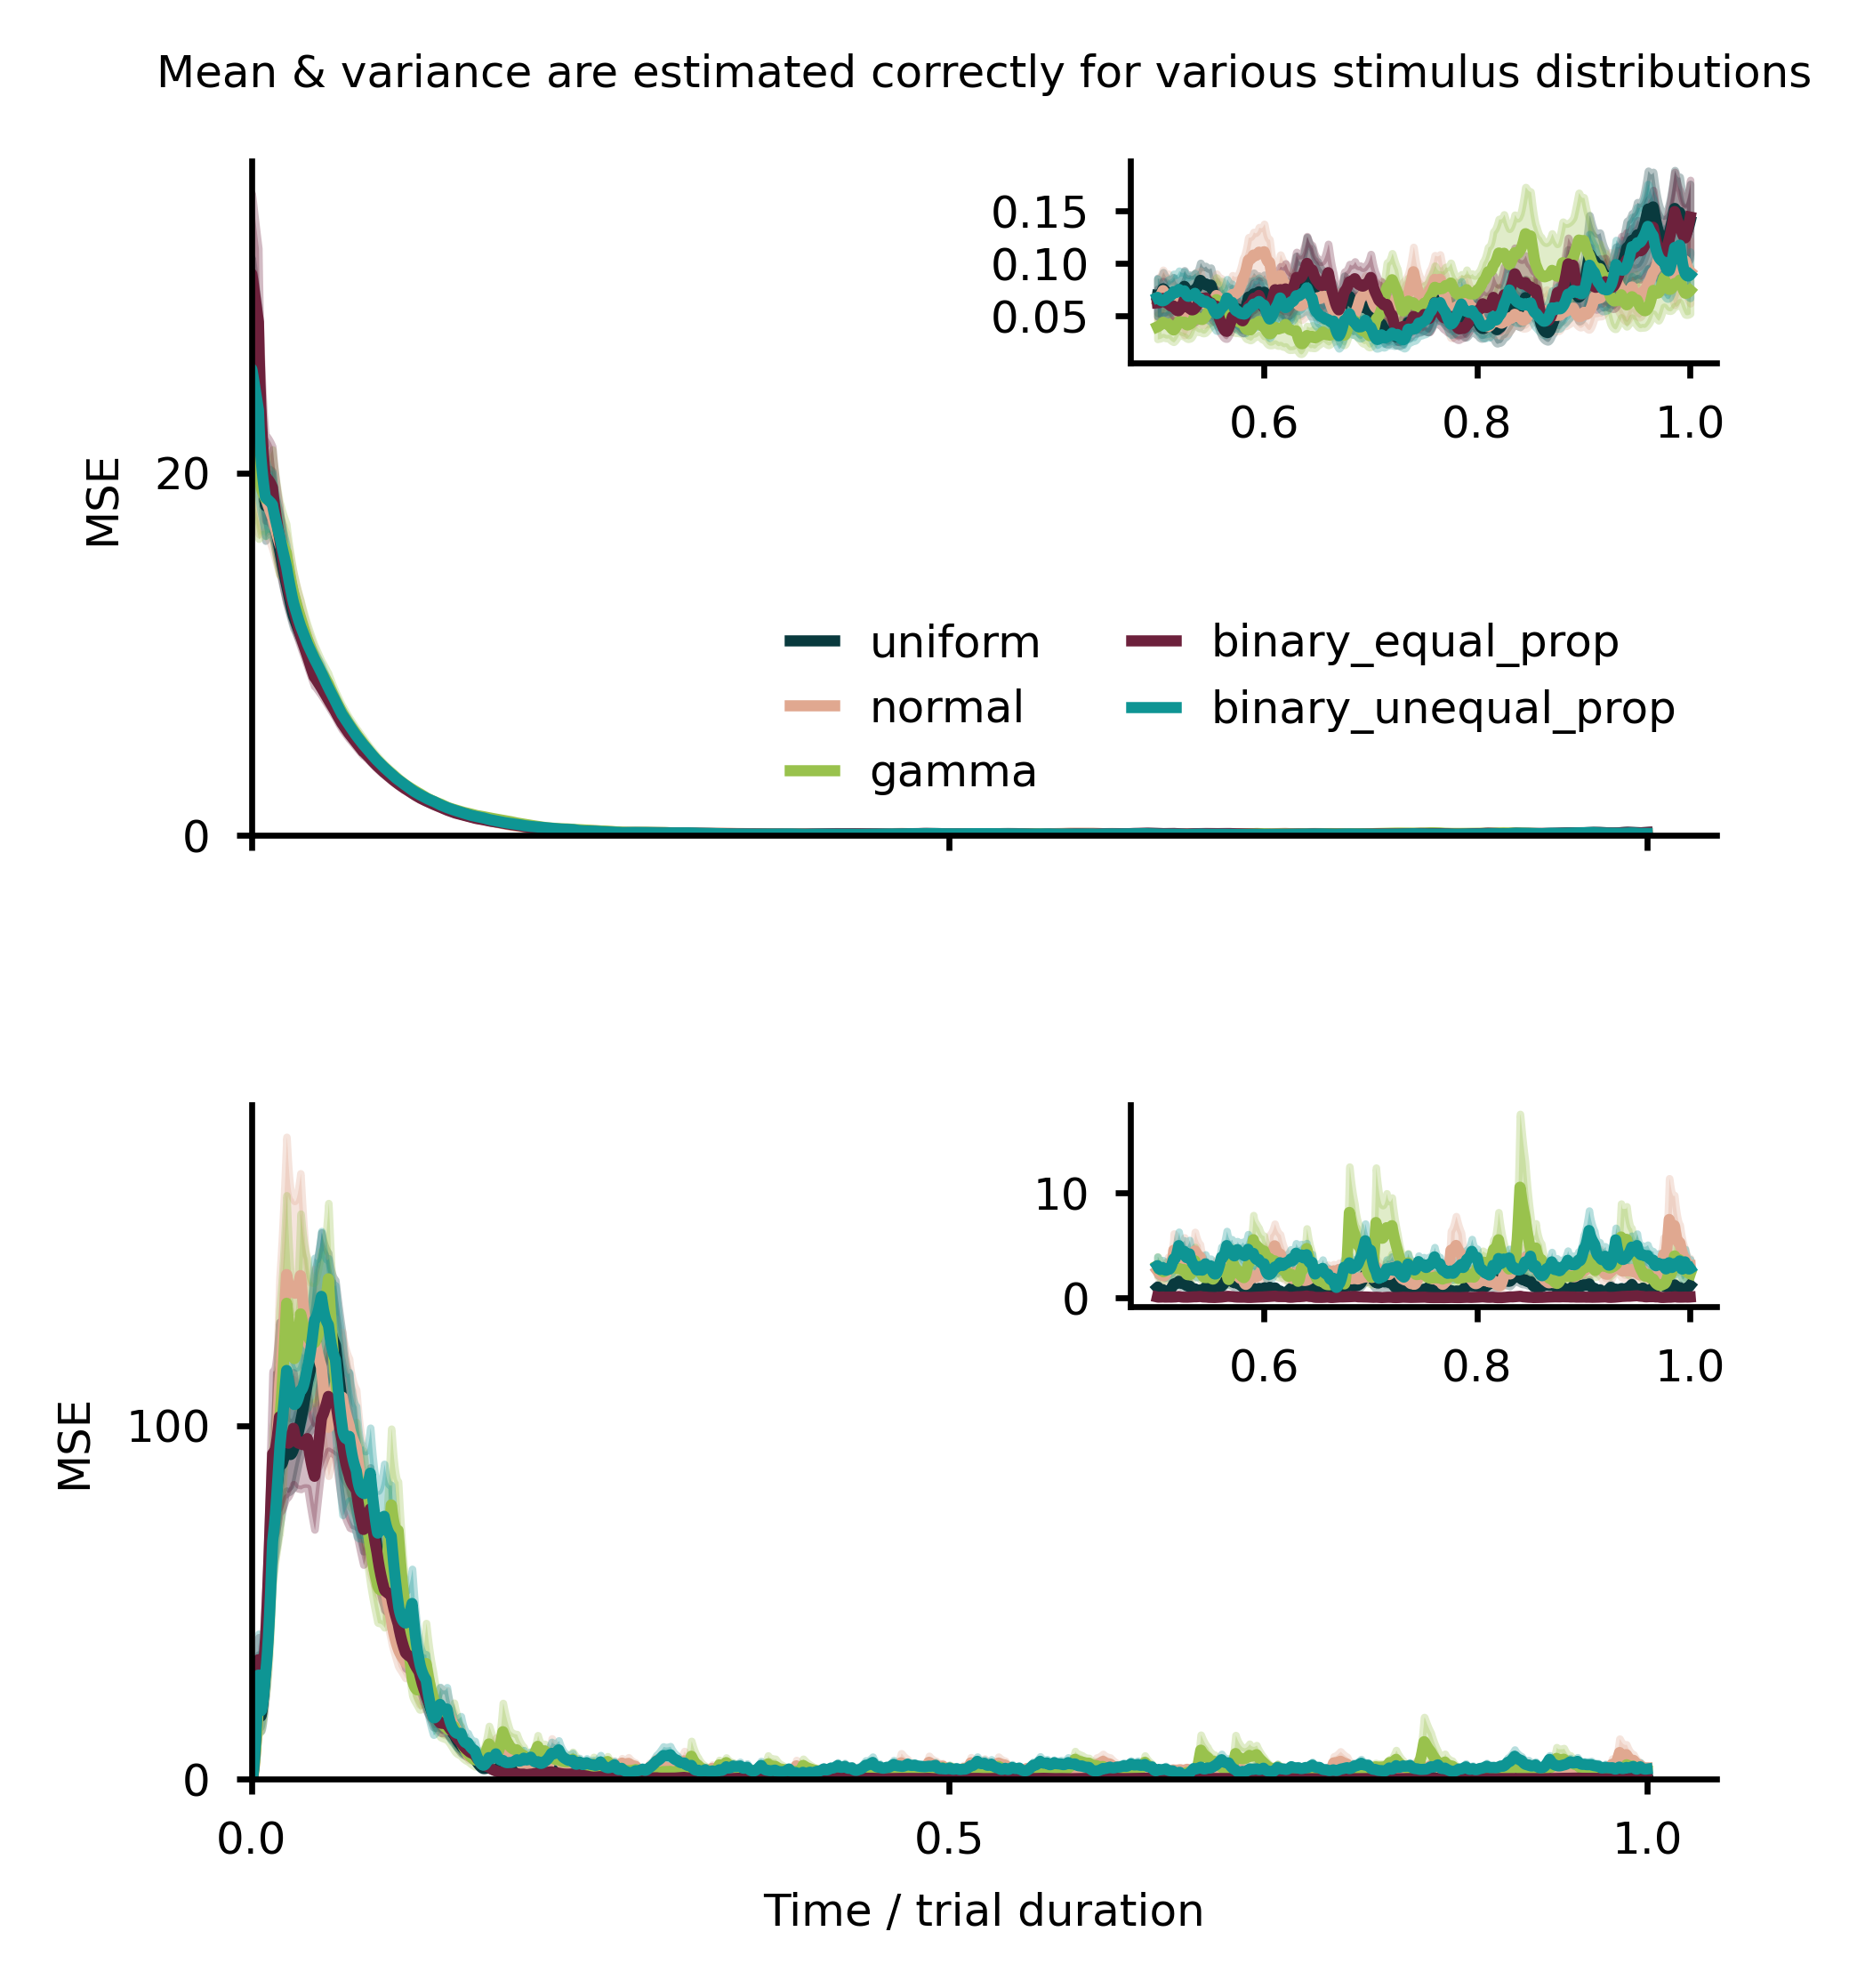
\includegraphics[scale=1]{../results/figures/final/Fig_2_S1}%%%
%DIF <  [width=1\linewidth]
%DIFDELCMD < \caption{%
{%DIFAUXCMD
%DIFDELCMD < \footnotesize{\bf Estimation of mean and variance for different stimulus distributions.\newline}  
%DIFDELCMD < %%%
\DIFdelFL{Top: The mean-squared error (MSE) between the running average and the activity of the M neuron decreases to a near-zero level for all stimulus distributions tested. 
Bottom: The MSE between the instantaneous variance and the V neuron decreases to a low level with minor differences between the distributions tested. Zoom-in shows the last half of the trial. Mean of the stimulus distribution = XXX, Variance of the stimulus distribution = XXX.
}}
%DIFAUXCMD
%DIFDELCMD < \label{fig:Fig_2_S1}
%DIFDELCMD < \end{figure}
%DIFDELCMD < %%%
\DIFdelend \DIFaddbegin \DIFadd{In recent years, normative models have been squared with biological constraints. For instance, in a paper by \mbox{%DIFAUXCMD
\cite{kutschireiter2023bayesian}}\hskip0pt%DIFAUXCMD
, uncertainty could be integrated into a ring attractor model encoding head direction. This }\textit{\DIFadd{Bayesian ring attractor}} \DIFadd{model encodes uncertainty in the amplitude of the network activity and matches the performance of a circular Kalman filter when the recurrent connections are tuned appropriately. In other seminal work, it has been proposed that Bayesian inference in time can be linked to the dynamics of leaky integrate-and-fire neurons with spike-dependent adaptation \mbox{%DIFAUXCMD
\citep{deneve2008bayesian}}\hskip0pt%DIFAUXCMD
.
}\DIFaddend 

\DIFdelbegin %DIFDELCMD < \begin{figure}[!h]
%DIFDELCMD < 	\centering
%DIFDELCMD <     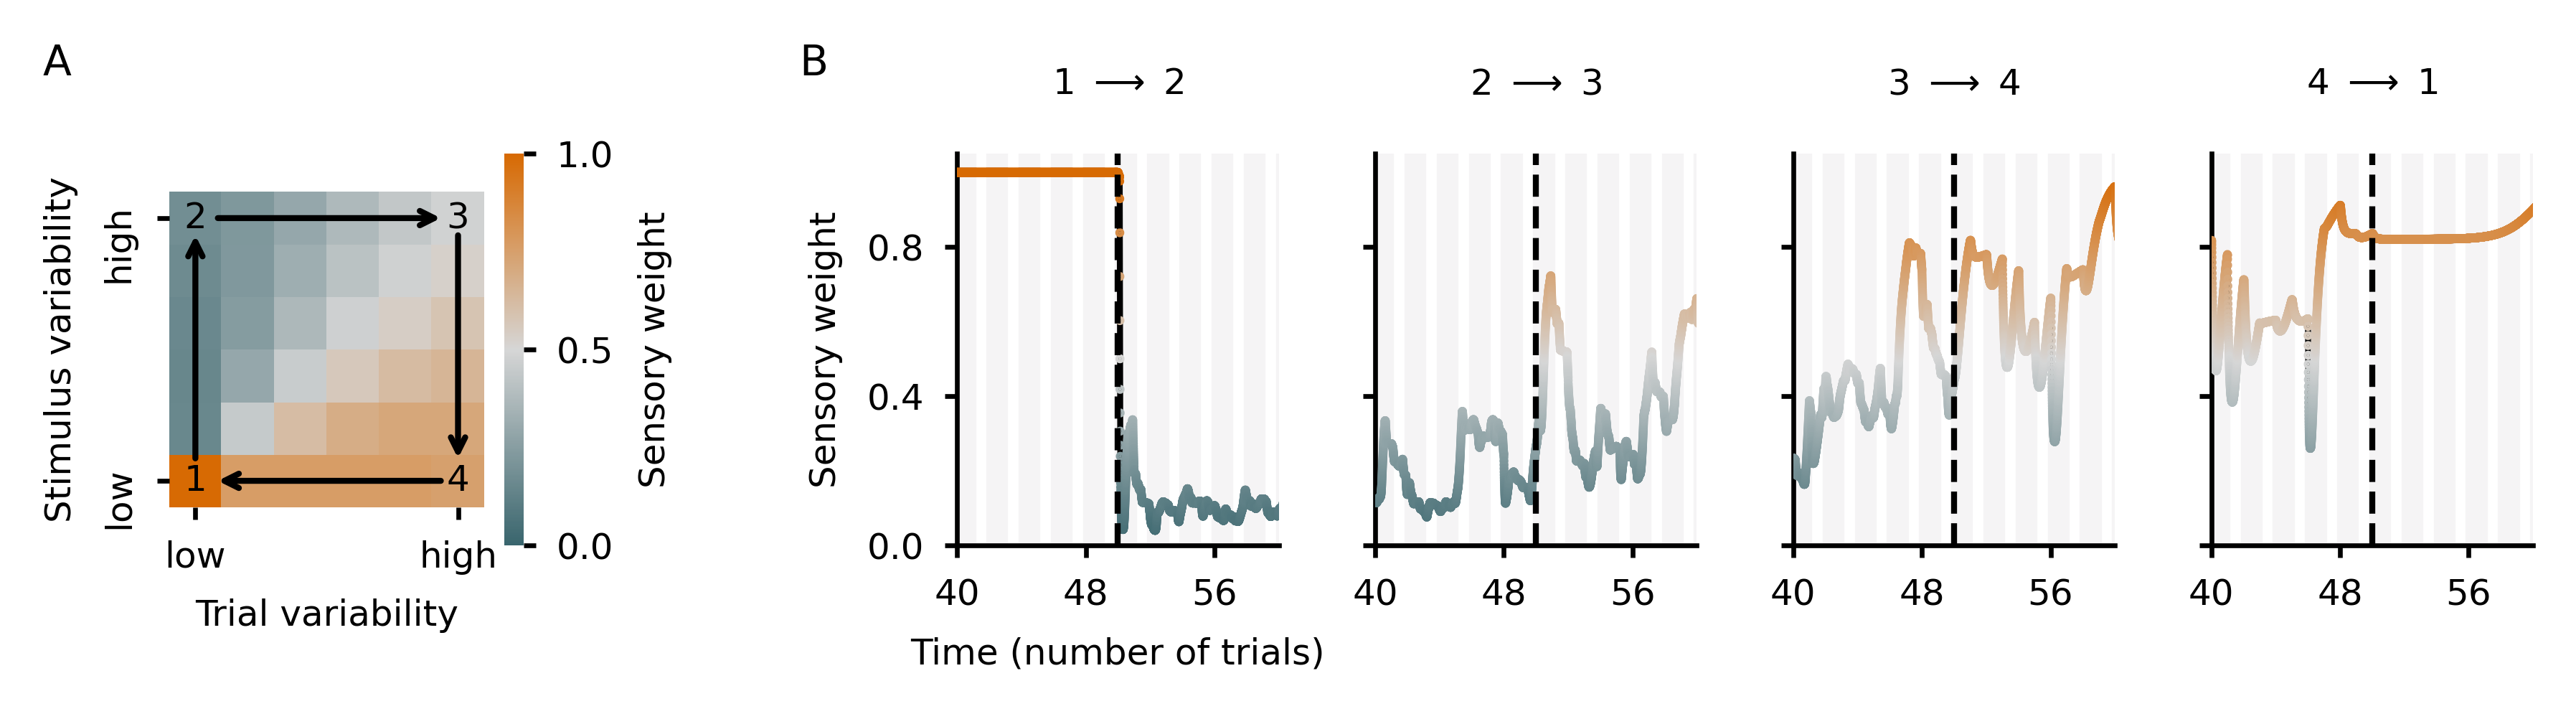
\includegraphics{../results/figures/final/Fig_3_S1}%%%
%DIF <  [width=1\linewidth]
%DIFDELCMD < \caption{%
{%DIFAUXCMD
%DIFDELCMD < \footnotesize{\bf Dynamic variance estimation allows flexible adaptation to changes in the stimulus statistics and environment. \newline}  
%DIFDELCMD < {\bf %%%
\DIFdelFL{(A)}%DIFDELCMD < } %%%
\DIFdelFL{Sensory weight for different input statistics (same as in Fig. \ref{fig:Fig_3}E). Numbers denote specific example states. Arrows denote the transitions between those states.
}%DIFDELCMD < {\bf %%%
\DIFdelFL{(B)}%DIFDELCMD < } %%%
\DIFdelFL{The sensory weight over time is shown for all transitions in (A). The switch to a new input statistics occurs at trial 60. Parameters are taken from Fig. \ref{fig:Fig_3}.
}}
%DIFAUXCMD
%DIFDELCMD < \label{fig:Fig_3_S1}
%DIFDELCMD < \end{figure}
%DIFDELCMD < %%%
\DIFdelend \DIFaddbegin \DIFadd{Here, we proposed an alternative view in which PE neurons serve as the backbone for estimating both the uncertainty of the feedforward sensory stimuli arising from the external world and the feedback signals carrying predictions about the same feedforward inputs our brains are bombarded with. Our work is an important step toward a better understanding of the brain’s ability to integrate these often unreliable feedforward and feedback signals that often do not match perfectly. 
}\DIFaddend 


\DIFdelbegin %DIFDELCMD < \begin{figure}[!h]
%DIFDELCMD < 	\centering
%DIFDELCMD <     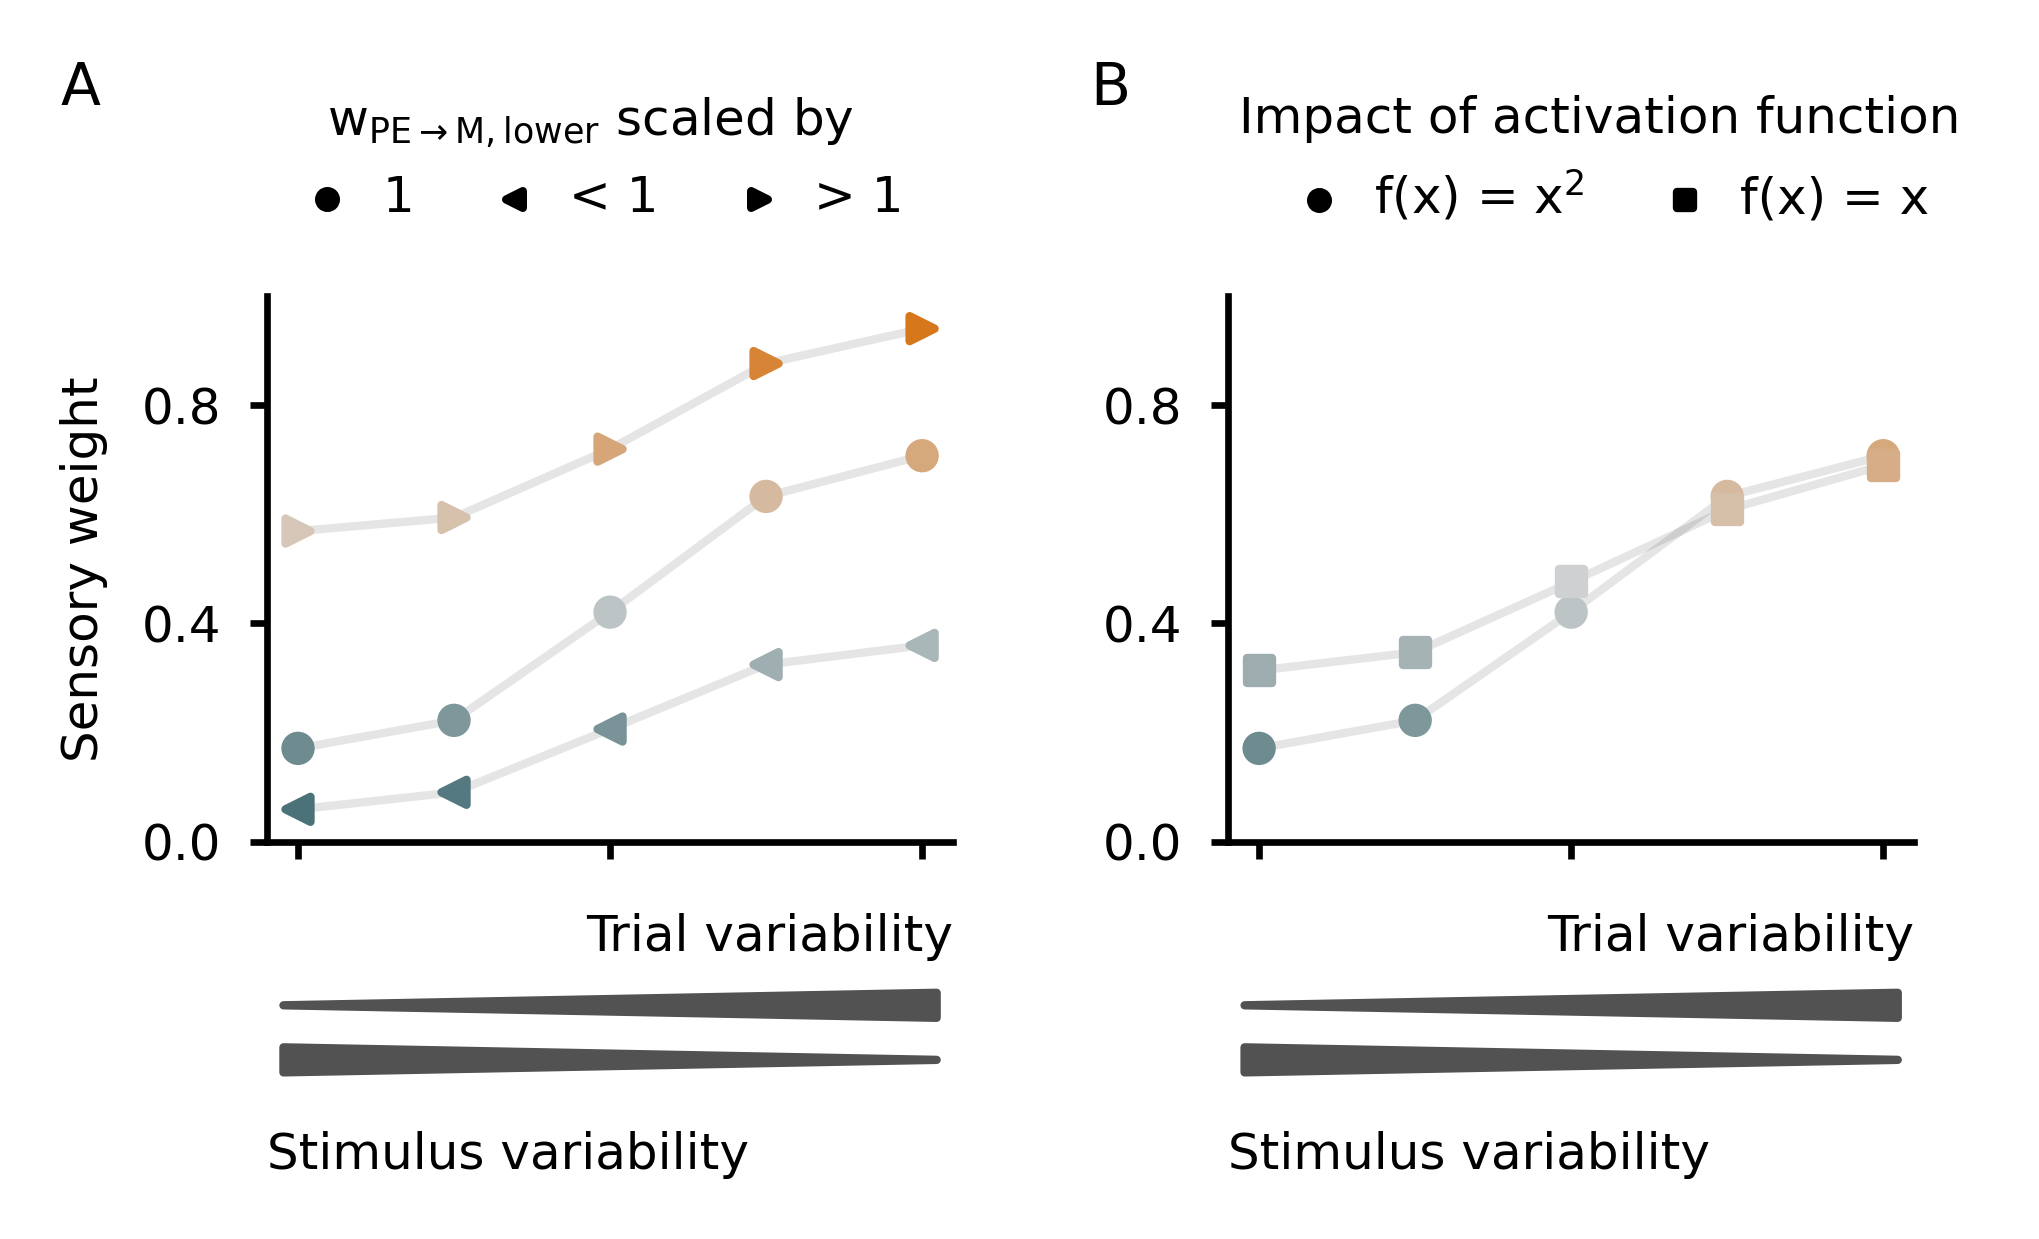
\includegraphics{../results/figures/final/Fig_3_S2}%%%
%DIF <  [width=1\linewidth]
%DIFDELCMD < \caption{%
{%DIFAUXCMD
%DIFDELCMD < \footnotesize{\bf Perturbing the weighting of sensory inputs and predictions by altering  network properties. \newline}  
%DIFDELCMD < {\bf %%%
\DIFdelFL{(A)}%DIFDELCMD < } %%%
\DIFdelFL{The weights from the lower-level PE neurons to the M neuron are scaled by a factor below 1 (here, xxx) or above 1 (here, xxx), leading to a distorted weighting. If the update of the M neuron in the lower subnetwork is too slow ($\blacktriangleleft$), the prediction is overrated. If the update of the M neuron in the lower subnetwork is too fast ($\blacktriangleright$), the sensory input is overrated.
}%DIFDELCMD < {\bf %%%
\DIFdelFL{(B)}%DIFDELCMD < } %%%
\DIFdelFL{The precise activation function for the V neurons does not have a major impact on the sensory weight. Only for inputs with high stimulus variability, the sensory stimulus is slightly overrated when the squared activation function is replaced by a linear, rectified activation function.
}}
%DIFAUXCMD
%DIFDELCMD < \label{fig:Fig_3_S2}
%DIFDELCMD < \end{figure}
%DIFDELCMD < %%%
\DIFdelend \DIFaddbegin \section*{\DIFadd{Models and methods}}
%DIF > 
\subsection*{\DIFadd{Network model}}
\DIFadd{The mean-field network model consists of a }\textit{\DIFadd{lower}} \DIFadd{and }\textit{\DIFadd{higher}} \DIFadd{PE circuit (Fig. \ref{fig:Fig_1}C-D). Each PE circuit contains an excitatory nPE neuron and pPE neuron ($\mathrm{N}_\mathrm{nPE} = \mathrm{N}_\mathrm{pPE} = 1$), as well as inhibitory neurons. The inhibitory neurons comprise PV, SOM and VIP neurons ($\mathrm{N}_\mathrm{SOM} = \mathrm{N}_\mathrm{VIP} = 1$, $\mathrm{N}_\mathrm{PV} = 2$). In addition to the core PE circuit, each subnetwork also includes one memory neuron $M$ and one variance neuron $V$. 
}\DIFaddend 

\DIFdelbegin %DIFDELCMD < \begin{figure}[!h]
%DIFDELCMD < 	\centering
%DIFDELCMD <     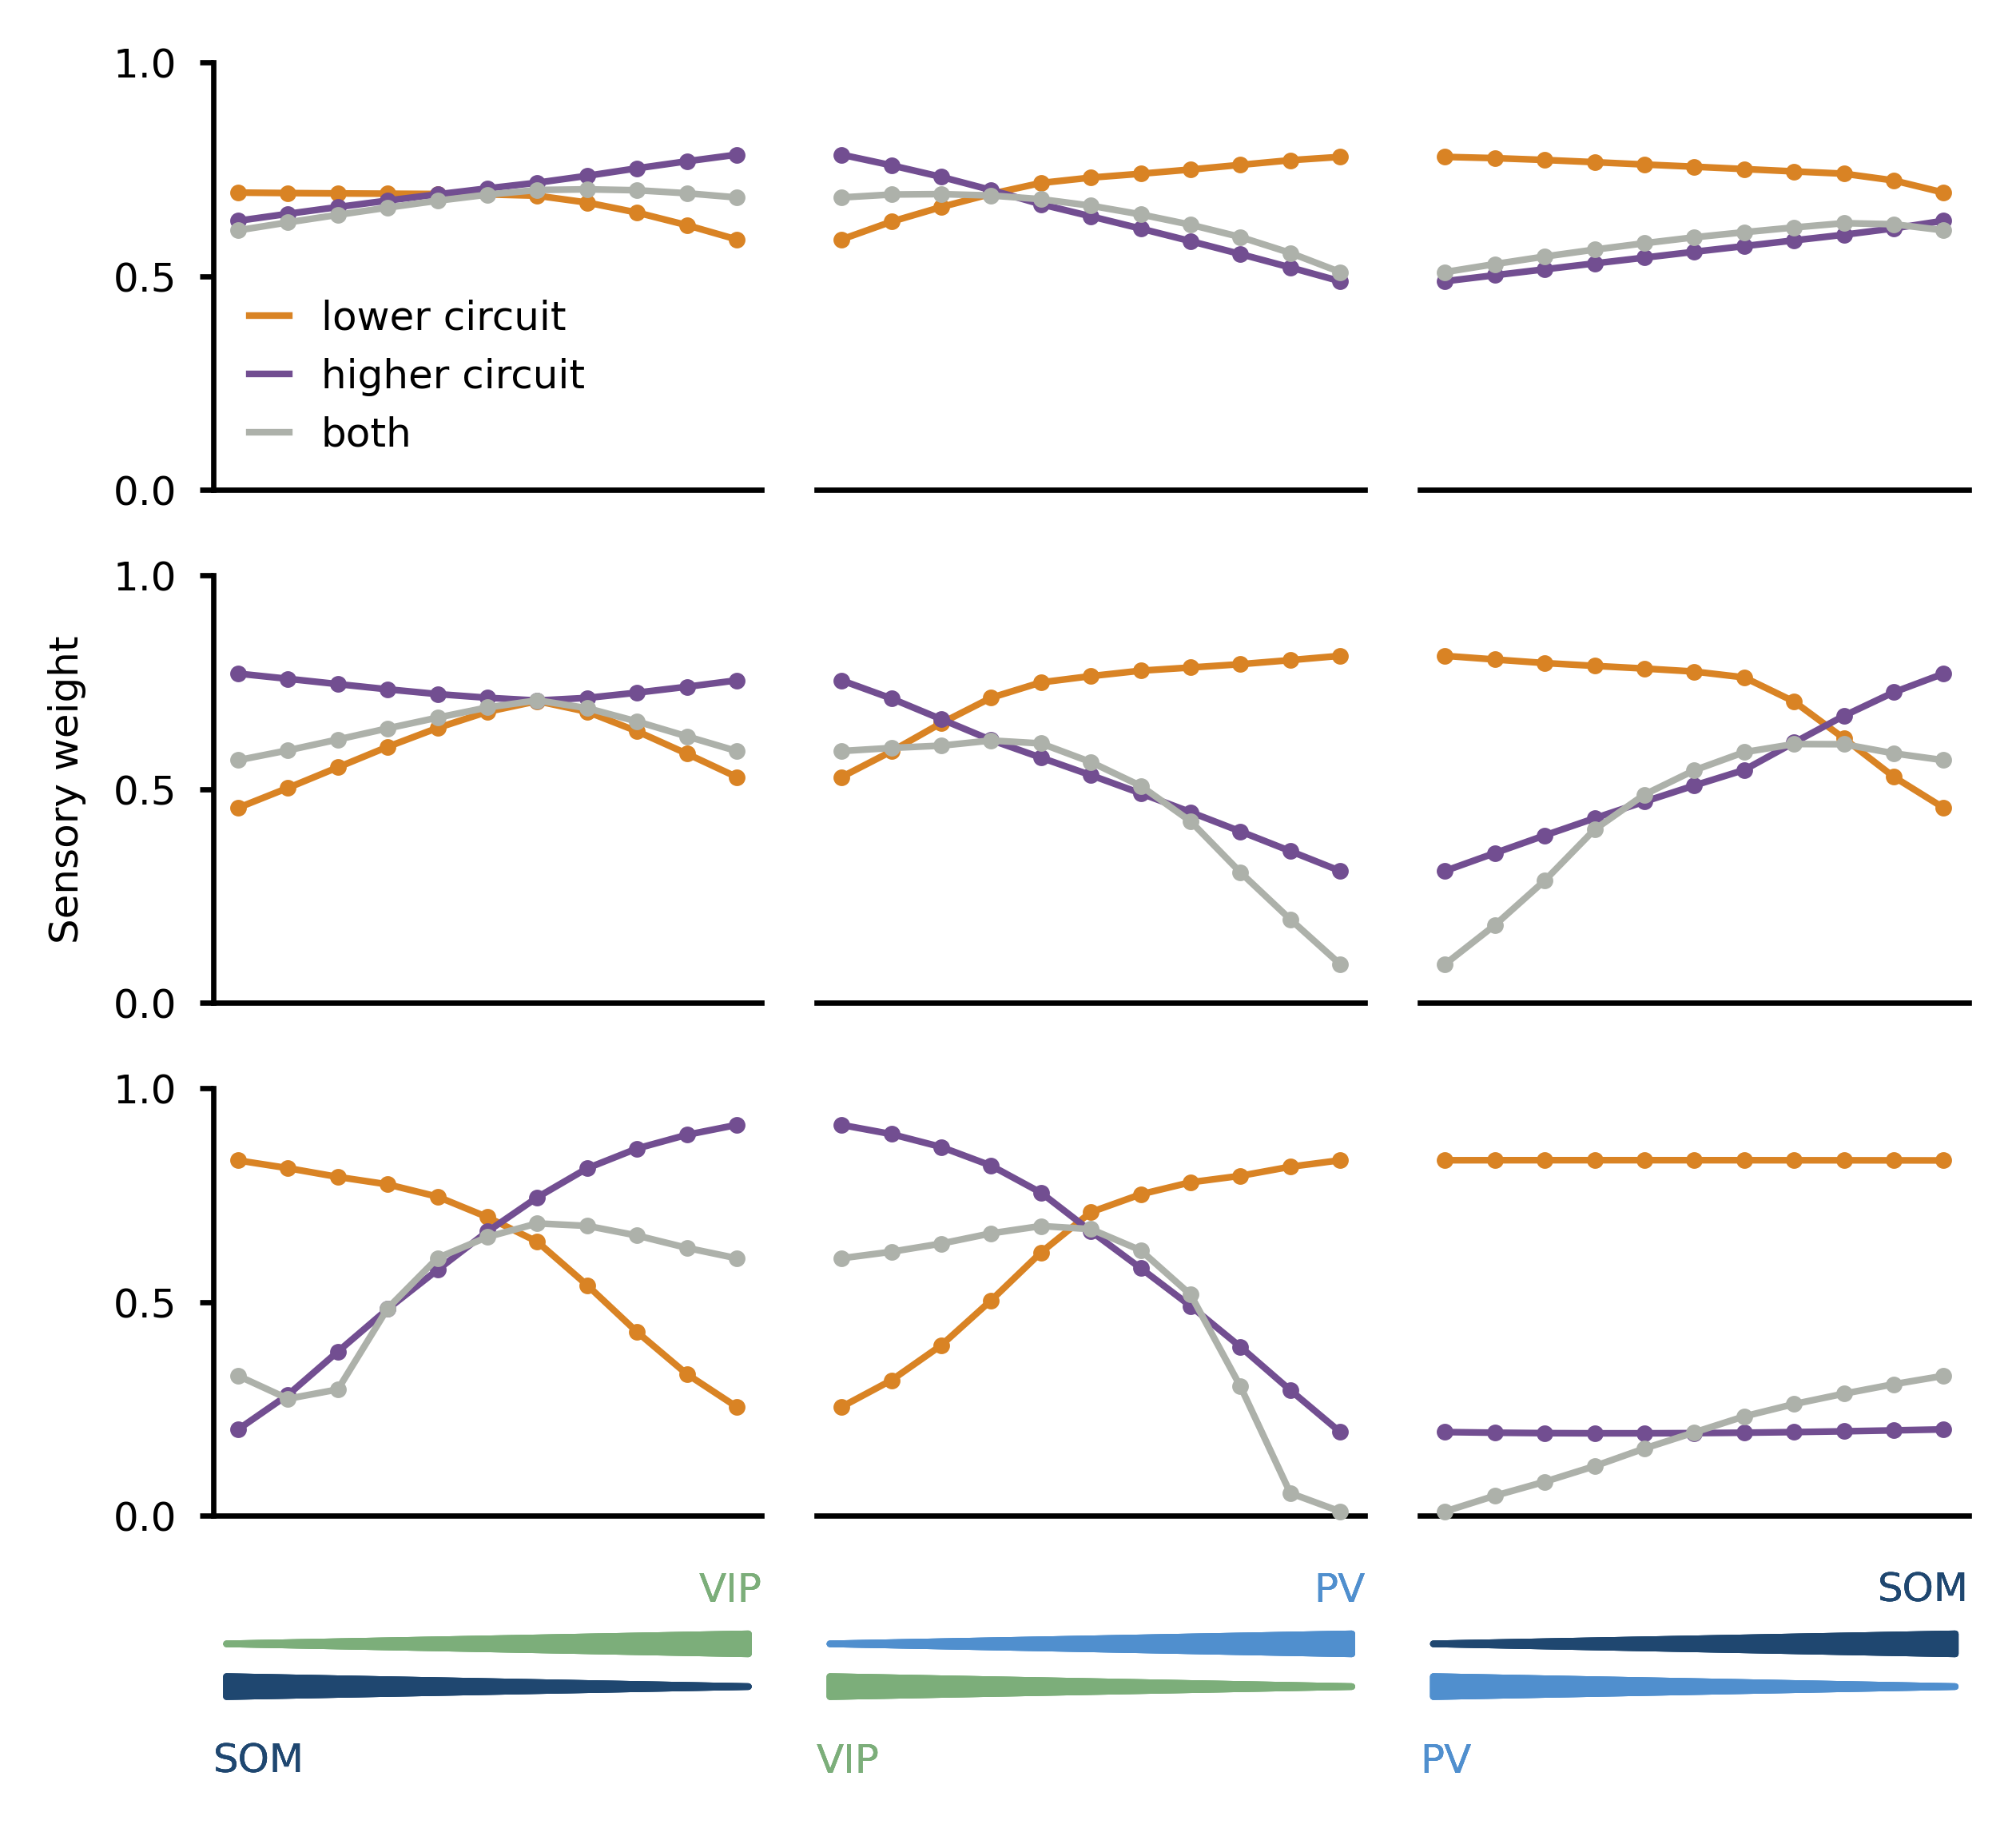
\includegraphics{../results/figures/final/Fig_4_S1}%%%
%DIF <  [width=1\linewidth]
%DIFDELCMD < \caption{\footnotesize{\bf Neuromodulators acting locally either on interneurons in the lower or higher PE circuit. \newline}  
%DIFDELCMD < {\bf %%%
\DIFdelFL{(A)}%DIFDELCMD < } %%%
\DIFdelFL{Sensory weight changes }\DIFdelendFL \DIFaddbeginFL \DIFaddFL{The excitatory neurons in the PE circuit are simulated as two coupled point compartments, representing the soma and the dendrites of elongated pyramidal cells. All other neurons are modeled as point neurons. The activities of all neurons are represented by a set of differential equations describing the network dynamics. 
}

\DIFaddFL{The dynamics of the neurons in the lower and higher PE circuits ($\underline{r}_\mathrm{PE}^\mathrm{low}$ and $\underline{r}_\mathrm{PE}^\mathrm{high}$) are given by
%DIF > 
}\begin{align}
\DIFaddFL{\underline{r}_\mathrm{PE}^\mathrm{low} = }& \DIFaddFL{\left[ \underline{h}_\mathrm{PE}^\mathrm{low} \right]_+ \nonumber}\\
%DIF > 
\DIFaddFL{\underline{r}_\mathrm{PE}^\mathrm{high} = }& \DIFaddFL{\left[ \underline{h}_\mathrm{PE}^\mathrm{high} \right]_+ 
}\end{align}
%DIF > 
\DIFaddendFL with
\DIFdelbeginFL \DIFdelFL{neuromodulators acting on interneurons in the lower PE circuit.
}%DIFDELCMD < {\bf %%%
\DIFdelFL{(B)}%DIFDELCMD < } %%%
\DIFdelFL{Sensory weight changes }\DIFdelendFL %DIF > 
\DIFaddbeginFL \begin{align}
\DIFaddFL{T \cdot \underline{\dot{h}}_\mathrm{PE}^\mathrm{low} =}& \DIFaddFL{-\underline{h}_\mathrm{PE}^\mathrm{low} + W_\mathrm{PE\leftarrow PE} \cdot \underline{r}_\mathrm{PE}^\mathrm{low} + \underline{w}_\mathrm{PE\leftarrow M} \cdot r_\mathrm{M}^\mathrm{low} + \underline{w}_\mathrm{PE\leftarrow FF} \cdot s + \underline{I}_\mathrm{PE} \nonumber}\\
%DIF > 
\DIFaddFL{T \cdot \underline{\dot{h}}_\mathrm{PE}^\mathrm{high} =}& \DIFaddFL{-\underline{h}_\mathrm{PE}^\mathrm{high} + W_\mathrm{PE\leftarrow PE} \cdot \underline{r}_\mathrm{PE}^\mathrm{high} + \underline{w}_\mathrm{PE\leftarrow M} \cdot r_\mathrm{M}^\mathrm{high} + \underline{w}_\mathrm{PE\leftarrow FF} \cdot r_\mathrm{M}^\mathrm{low} + \underline{I}_\mathrm{PE}.
%DIF > 
}\end{align}
%DIF > 
\DIFaddFL{We follow the notation that column and row vectors are indicated by letters with an underscore $\underline{\bullet}$, matrices are denoted by capital letters, and scalars are given by small letters without an underscore. Furthermore, a time derivative (e.g., $\frac{dx}{dt}$) is denoted by a dot above the letter (e.g., $\dot{x}$). The rate vector $\underline{r}_\mathrm{PE}^\mathrm{loc} = \left[r_\mathrm{nE}^\mathrm{loc},\ r_\mathrm{pE}^\mathrm{loc},\ r_\mathrm{nD}^\mathrm{loc},\ r_\mathrm{pD}^\mathrm{loc},\ r_\mathrm{PV_1}^\mathrm{loc}, r_\mathrm{PV_2}^\mathrm{loc},\ r_\mathrm{SOM}^\mathrm{loc}, r_\mathrm{VIP}^\mathrm{loc} \right]$  }\DIFaddendFL with \DIFdelbeginFL \DIFdelFL{neuromodulators acting on interneurons in the lower PE circuit}\DIFdelendFL \DIFaddbeginFL \DIFaddFL{$\mathrm{loc} \in [\mathrm{low}, \mathrm{high}]$ contains the activities of all neurons or compartments in the PE circuit (soma of nPE/pPE neurons: nE/pE, dendrites of nPE/pPE neurons: nD/pD). The network receives time-dependent stimuli $s$ and neuron/compartment-specific external background input $\underline{I}_\mathrm{PE}$. The connection strengths between the }\textit{\DIFaddFL{pre}}\DIFaddFL{-synaptic neuron (population) and the neurons of the PE circuit are denoted by $W_\mathrm{PE\leftarrow pre}$ and $\underline{w}_{\mathrm{PE} \leftarrow pre}$, respectively. The activities of the neurons evolve with time constants summarized in $T$}\DIFaddendFL .
\DIFdelbeginFL \DIFdelFL{Simulation parameters}\DIFdelendFL \DIFaddbeginFL 

\DIFaddFL{The activities of the lower and higher M neuron evolve according to a perfect integrator. The memory neurons receive synapses from both nPE and pPE neurons of the same subnetwork,
%DIF > 
}\begin{align}
\DIFaddFL{\dot{r}_\mathrm{M}^\mathrm{low} =}& \DIFaddFL{\underline{w}_\mathrm{M \leftarrow PE}^\mathrm{low} \cdot \underline{r}_\mathrm{PE}^\mathrm{low} = w_\mathrm{M \leftarrow pPE}^\mathrm{low} \cdot r_\mathrm{pPE}^\mathrm{low} - w_\mathrm{M \leftarrow nPE}^\mathrm{low} \cdot r_\mathrm{nPE}^\mathrm{low} \nonumber }\\
%DIF > 
\DIFaddFL{\dot{r}_\mathrm{M}^\mathrm{high} =}& \DIFaddFL{\underline{w}_\mathrm{M \leftarrow PE} ^\mathrm{high} \cdot \underline{r}_\mathrm{PE}^\mathrm{high} = w_\mathrm{M \leftarrow pPE}^\mathrm{high}  \cdot r_\mathrm{pPE}^\mathrm{high} - w_\mathrm{M \leftarrow nPE}^\mathrm{high}  \cdot r_\mathrm{nPE}^\mathrm{high} .
}\end{align}
%DIF > 

\DIFaddFL{The activities of the lower and higher V neuron evolve according to a leaky integrator with quadratic activation function. The variance neurons receive synapses from both nPE and pPE neurons of the same subnetwork,
%DIF > 
}\begin{align}
\DIFaddFL{\tau_\mathrm{V}^\mathrm{low} \cdot \dot{r}_\mathrm{V}^\mathrm{low} =}& \DIFaddFL{- r_\mathrm{V}^\mathrm{low} + \left( \underline{w}_\mathrm{V \leftarrow PE} \cdot \underline{r}_\mathrm{PE}^\mathrm{low}\right)^2 = - r_\mathrm{V}^\mathrm{low} + \left( w_\mathrm{V \leftarrow pPE} \cdot r_\mathrm{pPE}^\mathrm{low}\ + w_\mathrm{V \leftarrow nPE} \cdot r_\mathrm{nPE}^\mathrm{low}\right)^2 \nonumber}\\
%DIF > 
\DIFaddFL{\tau_\mathrm{V}^\mathrm{high} \cdot \dot{r}_\mathrm{V}^\mathrm{high} =}& \DIFaddFL{- r_\mathrm{V}^\mathrm{high} + \left( \underline{w}_\mathrm{V \leftarrow PE} \cdot \underline{r}_\mathrm{PE}^\mathrm{high}\right)^2 = - r_\mathrm{V}^\mathrm{high} + \left( w_\mathrm{V \leftarrow pPE} \cdot r_\mathrm{pPE}^\mathrm{high}\ + w_\mathrm{V \leftarrow nPE} \cdot r_\mathrm{nPE}^\mathrm{high}\right)^2.
}\end{align} 
%DIF > 
\DIFaddFL{All values for neuron and network parameters, details on the model equations for the mean-field and the population network, as well as supporting analyses can be found in the supplementary material.
}

\subsection*{\DIFaddFL{Weighting of sensory inputs and predictions}}
%DIF > 
\DIFaddFL{We arithmetically calculated the weighted output of sensory inputs and predictions, $r_\mathrm{out}$, based on ideas of Bayesian multisensory integration \mbox{%DIFAUXCMD
\citep[see, e.g.][]{pouget2013probabilistic}}\hskip0pt%DIFAUXCMD
,
%DIF > 
}\begin{align}
\DIFaddFL{r_\mathrm{out} = \alpha \cdot s + (1-\alpha) \cdot r_\mathrm{M}^\mathrm{low},
}\end{align}
%DIF > 
\DIFaddFL{where $\alpha$ denotes the sensory weight (that is, the reliability of the sensory input) and is given by 
%DIF > 
}\begin{align}
\DIFaddFL{\alpha }&\DIFaddFL{= \left( 1 + \frac{r_\mathrm{V}^\mathrm{low}}{r_\mathrm{V}^\mathrm{high}} \right)^{-1}.
}\end{align}


\subsection*{\DIFaddFL{Inputs}}
%DIF > 
\DIFaddFL{The network receives feedforward stimuli $s$ that may vary between trials. To account for noise, each stimulus is composed of N$_\mathrm{in}$ consecutive, piece-wise constant values drawn from a normal distribution with mean $\mu_\mathrm{in}$ and standard deviation $\sigma_\mathrm{in}$. To account for changes in the environment, $\mu_\mathrm{in}$ is drawn from a uniform distribution $U(a,b)$ with mean $\mu_\mathrm{trial} = \frac{a+b}{2}$ and standard deviation $\sigma_\mathrm{trial} = \frac{b-a}{\sqrt{12}}$. The parameterization of both distributions varies across the experiments. All stimulus/input parameters can be found in the supplementary material.
}

\subsection*{\DIFaddFL{Simulations}}
%DIF > 
\DIFaddFL{All simulations were performed in customized Python code written by LH. Source code to reproduce the simulations, analyses, and figures will be available after publication at }\url{https://github.com/lhertaeg/weighted_sensory_prediction}\DIFaddFL{. Differential equations were numerically integrated using a 2\textsuperscript{nd}-order Runge-Kutta method. Neurons were initialized with $r=0/s$. Further details and values for simulation parameters can be found in the supplementary material.
}


\section*{\DIFaddFL{Acknowledgments}}
%DIF > 
%DIF > We are grateful to Vezha Boboeva, Douglas Feitosa Tom\'e, J\'ulia Gallinaro and Klara Kaleb for helpful comments on earlier versions of this manuscript, and we want to thank all members of the Clopath lab for discussion and support. This work was supported by BBSRC BB/N013956/1, BB/N019008/1, Wellcome Trust 200790/Z/16/Z, Simons Foundation 564408 and EPSRC EP/R035806/1.

%DIF > \bibliographystyle{naturemag} %{plainnat}
\bibliographystyle{plainnat}
\bibliography{References_HertaegWilmesClopath_2023}



%DIF > %%%%%%%%%%%%%%%%%%%%%%%%%%%%%%%%%%%%%%%%%%%%%%%%%%%%%%%%%%%
%DIF > %% APPENDICES
%DIF > %%%%%%%%%%%%%%%%%%%%%%%%%%%%%%%%%%%%%%%%%%%%%%%%%%%%%%%%%%%


\clearpage
\appendix


\tableofcontents
\section{\DIFaddFL{Detailed Methods}}
%DIF > 
\DIFaddFL{In the following, we describe in more detail the equations for the dynamics of the neurons in the prediction-error circuit, as well as the memory and variance neurons. We then provide the connectivity of the network and the inputs to the neurons for both the mean-field and population model. Finally, to ensure reproducibility, we summarize all simulation parameters used for the results shown in the figures.  
}

\subsection{\DIFaddFL{Network model}}
%DIF > 
\DIFaddFL{The network model consists of a }\textit{\DIFaddFL{lower}} \DIFaddFL{and }\textit{\DIFaddFL{higher}} \DIFaddFL{mean-field PE circuit (Fig. \ref{fig:Fig_1}). Each PE circuit contains an excitatory nPE neuron and pPE neuron ($\mathrm{N}_\mathrm{nPE} = \mathrm{N}_\mathrm{pPE} = 1$), as well as inhibitory neurons. The inhibitory neurons comprise PV, SOM and VIP neurons ($\mathrm{N}_\mathrm{SOM} = \mathrm{N}_\mathrm{VIP} = 1$}\DIFaddendFL , \DIFdelbeginFL \DIFdelFL{labels }\DIFdelendFL \DIFaddbeginFL \DIFaddFL{$\mathrm{N}_\mathrm{PV} = 2$). In addition to the core PE circuit, each subnetwork also includes one memory neuron $M$ and one variance neuron $V$. 
}

\DIFaddFL{In Figure \ref{fig:Fig_2} and the corresponding supporting figures, only the lower subnetwork is simulated. In Fig. \ref{fig:Fig_2_S2}, we replaced this lower mean-field PE circuit with a heterogeneous population model containing $200$ neurons ($\mathrm{N}_\mathrm{SOM} = \mathrm{N}_\mathrm{VIP} = \mathrm{N}_\mathrm{PV} = 20$, $140$ excitatory neurons). In Fig. \ref{fig:Fig_2_S3}, the lower PE circuit comprises $1000$ copies of the mean-field network to account for selectivity.
}

\DIFaddFL{In the following, we describe the dynamics of the neurons/compartments in the mean-field network. The equations for the population PE circuit (Fig. \ref{fig:Fig_2_S2}) are directly deduced from the mean-field equations and can also be found in \mbox{%DIFAUXCMD
\citep{hertag2022prediction}}\hskip0pt%DIFAUXCMD
.
}

\subsubsection{\DIFaddFL{Prediction-error network model}}
%DIF > 
\DIFaddFL{Each excitatory pyramidal cell (that is, nPE or pPE neuron) is divided into two coupled compartments, representing the soma and the dendrites, respectively. The dynamics of the firing rates of the somatic compartments~$r_{\mathrm{nE}}$ (nPE neuron) and~$r_{\mathrm{pE}}$ (pPE neuron) obey \mbox{%DIFAUXCMD
\citep{wilson1972excitatory}
}\hskip0pt%DIFAUXCMD
%DIF > 
}\begin{align}
\DIFaddFL{r_\mathrm{nE} = }[\DIFaddFL{h_\mathrm{nE}}]\DIFaddFL{_+ \ \mbox{ with }\ \tau_E\ \frac{dh_\mathrm{nE}}{dt} }&\DIFaddFL{= - h_\mathrm{nE} + w_\mathrm{nE\leftarrow nD}\cdot  r_\mathrm{nD}  -  w_\mathrm{nE\leftarrow PV_1}\cdot r_\mathrm{PV_1}  -  w_\mathrm{nE\leftarrow PV_2}\cdot r_\mathrm{PV_2} + I_\mathrm{nE}, \nonumber}\\
\DIFaddFL{r_\mathrm{pE} = }[\DIFaddFL{h_\mathrm{pE}}]\DIFaddFL{_+ \ \mbox{ with }\ \tau_E\ \frac{dh_\mathrm{pE}}{dt} }&\DIFaddFL{= - h_\mathrm{pE} + w_\mathrm{pE\leftarrow pD}\cdot  r_\mathrm{pD}  -  w_\mathrm{pE\leftarrow PV_1}\cdot r_\mathrm{PV_1}  -  w_\mathrm{pE\leftarrow PV_2}\cdot r_\mathrm{PV_2} + I_\mathrm{pE}
}\end{align}
%DIF > 
\DIFaddFL{where $\tau_\mathrm{E}$ denotes the excitatory rate time constant ($\tau_\mathrm{E}$=60 ms), the weights $w_{\mathrm{nE\leftarrow nD}}$ }\DIFaddendFL and \DIFdelbeginFL \DIFdelFL{colors as in Fig}\DIFdelendFL \DIFaddbeginFL \DIFaddFL{$w_{\mathrm{pE\leftarrow pD}}$ describe the connection strength between the dendritic compartment and the soma of the same neuron, and $w_{\mathrm{nE\leftarrow PV_1}}$, $w_{\mathrm{nE\leftarrow PV_2}}$, $w_{\mathrm{pE\leftarrow PV_1}}$ and $w_{\mathrm{pE\leftarrow PV_2}}$ denote the strength of somatic inhibition from PV neurons. The overall input $I_\mathrm{nE}$ and $I_\mathrm{pE}$ comprise the external background and feedforward inputs (see ``Inputs" below). Firing rates are rectified to ensure positivity ($[\bullet]_+$). 
}

\DIFaddFL{The dynamics of the activity of the dendritic compartments~$r_\mathrm{nD}$ (nPE neuron) and~$r_\mathrm{pD}$ (pPE neuron) obey \mbox{%DIFAUXCMD
\citep{wilson1972excitatory}
}\hskip0pt%DIFAUXCMD
%DIF > 
}\begin{align}
\DIFaddFL{r_\mathrm{nD} = }[\DIFaddFL{h_\mathrm{nD}}]\DIFaddFL{_+ \ \mbox{ with }\ \tau_E\ \frac{dh_\mathrm{nD}}{dt} =}& \DIFaddFL{- h_\mathrm{nD} +  w_\mathrm{nD\leftarrow nE}\cdot r_\mathrm{nE} +  w_\mathrm{nD\leftarrow pE}\cdot r_\mathrm{pE} + w_\mathrm{nD\leftarrow M}\cdot  r_\mathrm{M} \nonumber}\\
& \DIFaddFL{- w_\mathrm{nD\leftarrow SOM}\cdot r_\mathrm{SOM} + I_\mathrm{nD}, \nonumber}\\
\DIFaddFL{r_\mathrm{pD} = }[\DIFaddFL{h_\mathrm{pD}}]\DIFaddFL{_+ \ \mbox{ with }\ \tau_E\ \frac{dh_\mathrm{pD}}{dt} =}& \DIFaddFL{- h_\mathrm{pD} +  w_\mathrm{pD\leftarrow nE}\cdot r_\mathrm{pE} +  w_\mathrm{pD\leftarrow pE}\cdot r_\mathrm{pE}+ w_\mathrm{pD\leftarrow M}\cdot  r_\mathrm{M}  \nonumber}\\
&\DIFaddFL{- w_\mathrm{pD\leftarrow SOM}\cdot r_\mathrm{SOM} + I_\mathrm{pD},
}\end{align}
%DIF > 
\DIFaddFL{where the weights $w_{\mathrm{nD\leftarrow nE}}$, $w_{\mathrm{nD\leftarrow pE}}$, $w_{\mathrm{pD\leftarrow nE}}$ and $w_{\mathrm{pD\leftarrow pE}}$ denote the recurrent excitatory connections between PCs, including backpropagating activity from the soma to the dendrites. $w_{\mathrm{nD\leftarrow SOM}}$ and $w_{\mathrm{pD\leftarrow SOM}}$ represent the strength of dendritic inhibition from the SOM neuron. $w_{\mathrm{nD\leftarrow M}}$ and $w_{\mathrm{pD\leftarrow M}}$ denote the strength of connection between the memory neuron and the dendrites. The overall inputs $I_\mathrm{nD}$ and $I_\mathrm{pD}$ comprise fixed, external background inputs (see ``Inputs" below). We assume that any excess of inhibition in a dendrite does not affect the soma, that is, the dendritic compartment is rectified at zero. 
}

\DIFaddFL{Similarly, the firing rate dynamics of each interneuron is modeled by a rectified, linear differential equation,
%DIF > 
}\begin{align}
\DIFaddFL{\label{eq:RateEqINs}
r_\mathrm{X} = }[\DIFaddFL{h_\mathrm{X}}]\DIFaddFL{_+ \ \mbox{ with }\ \tau_I\ \frac{dh_\mathrm{X}}{dt} =}& \DIFaddFL{-h_\mathrm{X} + I_{\mathrm{X}} + w_\mathrm{X\leftarrow nE}\cdot r_\mathrm{nE} + w_\mathrm{X\leftarrow pE}\cdot r_\mathrm{pE}  +  w_\mathrm{X\leftarrow M}\cdot  r_\mathrm{M} - w_\mathrm{X\leftarrow PV_1}\cdot r_\mathrm{PV_1}  \nonumber}\\
&\DIFaddFL{- w_\mathrm{X\leftarrow PV_2}\cdot r_\mathrm{PV_2}  - w_\mathrm{X\leftarrow SOM}\cdot r_\mathrm{SOM} -  w_\mathrm{X\leftarrow VIP}\cdot r_\mathrm{VIP},
}\end{align}
%DIF > 
\DIFaddFL{where $r_\mathrm{X}$ denotes the firing rate of interneuron type $X$, and the weight $w_\mathrm{X\leftarrow Y}$ denotes the strength of connection between the presynaptic neuron $Y$ and the postsynaptic neuron $X$ ($X \in \lbrace \mathrm{PV_1}, \mathrm{PV_2}, \mathrm{SOM}, \mathrm{VIP}\rbrace$, $Y\in \lbrace \mathrm{nPE}, \mathrm{pPE}, \mathrm{PV_1}, \mathrm{PV_2}, \mathrm{SOM}, \mathrm{VIP}, \mathrm{M}\rbrace$). The rate time constant $\tau_I$ was chosen to resemble a fast GABA\textsubscript{A} time constant, and set to 2 ms for all interneuron types included. The overall input $I_\mathrm{X}$ comprises fixed, external background inputs and feedforward sensory inputs (see ``Inputs" below).
}

\subsubsection{\DIFaddFL{Memory and variance neuron}}
%DIF > 
\DIFaddFL{In addition to the core PE circuit, we simulate a memory neuron }\textit{\DIFaddFL{M}} \DIFaddFL{and a variance neuron }\textit{\DIFaddFL{V}}\DIFaddFL{. The memory neuron is modeled as a perfect integrator, receiving synapses from both the nPE and pPE neuron,
%DIF > 
}\begin{align}
\DIFaddFL{\tau_E \cdot \frac{dr_\mathrm{M}}{dt} = w_\mathrm{M\leftarrow pE} \cdot r_\mathrm{pE} - w_\mathrm{M\leftarrow nE} \cdot r_\mathrm{nE}.
}\end{align}
%DIF > 
\DIFaddFL{$w_\mathrm{M\leftarrow pE}$ denotes the connection strength between the pPE neuron and the memory neuron, and  $w_\mathrm{M\leftarrow nE}$ denotes the connection strength between the nPE neuron and the memory neuron. The time constant $\tau_E = 60$ ms.
}

\DIFaddFL{The dynamics of the variance neuron obeys a non-linear differential equation with leak term,
%DIF > 
}\begin{align}
\DIFaddFL{\tau_V \cdot \frac{dr_\mathrm{V}}{dt} = -r_\mathrm{V} + (w_\mathrm{V\leftarrow pE} \cdot r_\mathrm{pE} + w_\mathrm{V\leftarrow nE} \cdot r_\mathrm{nE})^2.
}\end{align}
%DIF > 
\DIFaddFL{The weight $w_\mathrm{V\leftarrow pE}$ represents the connection strength between the pPE neuron and the variance neuron, while  $w_\mathrm{V\leftarrow nE}$ denotes the connection strength between the nPE neuron and the variance neuron. To ensure that the V neuron encodes the variance, we chose a quadratic activation function. In Fig. \ref{fig:Fig_3_S2}, we used a linear activation function to investigate the impact of the input-output transfer function on the weighting of sensory inputs and predictions. The time constant $\tau_V$ was 5 s in the mean-field model, 2~s in the heterogeneous population model (Fig. \ref{fig:Fig_2_S2}), and 0.5~s in the population model with selectivity (Fig. \ref{fig:Fig_2_S3}).
}

\subsubsection{\DIFaddFL{Weighted output}}
%DIF > 
\DIFaddFL{The weighted output $r_\mathrm{out}(t) $ is a linear combination of the current sensory input $s(t)$ and the activity of the memory neuron, $r_\mathrm{M}(t)$, inspired by Bayesian multisensory integration \mbox{%DIFAUXCMD
\citep[see, e.g.][]{pouget2013probabilistic}}\hskip0pt%DIFAUXCMD
,
%DIF > 
}\begin{align}
\DIFaddFL{r_\mathrm{out}(t) = \alpha \cdot s(t) + (1-\alpha) \cdot r_\mathrm{M}(t).
}\end{align}
%DIF > 
\DIFaddFL{How strongly either the sensory input or the prediction thereof contributes to the output is denoted by the sensory weight $\alpha$,
%DIF > 
}\begin{align}
\DIFaddFL{\alpha }&\DIFaddFL{= \frac{r_\mathrm{V_{lower}}^{-1}}{r_\mathrm{V_{lower}}^{-1} + r_\mathrm{V_{higher}}^{-1}}\nonumber}\\
& \DIFaddFL{= \left( 1 + \frac{r_\mathrm{V_{lower}}}{r_\mathrm{V_{higher}}} \right)^{-1}.
}\end{align}

\subsection{\DIFaddFL{Connectivity}}
%DIF > 
%DIF > 
\subsubsection{\DIFaddFL{Connections between neurons of the PE circuit}}
%DIF > 
\DIFaddFL{The connectivity between neurons of the PE circuit, both for the mean-field and the population network, were taken from \mbox{%DIFAUXCMD
\citep{hertag2022prediction}}\hskip0pt%DIFAUXCMD
. We considered three mean-field networks (see Table \ref{tab:wXM}) that differed in terms of the inputs (feedforward vs. feedback) onto the SOM and VIP neurons, and, hence, in their connectivity that established an E/I balance in the excitatory neurons.
}

\subsubsection{\DIFaddFL{Connections between the PE circuit and the M neuron}}
%DIF > 
\DIFaddFL{While the nPE neurons inhibit the M neuron, the pPE neurons excite it. To ensure that the activities of the memory neurons represent the mean of the sensory stimuli in the lower PE circuit and the mean of the prediction in the higher subnetwork, respectively, the net effect of nPE and pPE neurons must cancel in the steady state (see Analysis in \ref{sec:gain_impact}). Hence, the weights need to account for the neurons' potentially different gain factors ($g_\mathrm{nPE}$ and $g_\mathrm{pPE}$) and the neuron numbers ($N_\mathrm{nPE}$ and $N_\mathrm{pPE}$):
%DIF > 
}\begin{align*}
\DIFaddFL{w_\mathrm{M\leftarrow nE}\  }&\DIFaddFL{=\ \frac{-\lambda}{g_\mathrm{nPE} \cdot N_\mathrm{nPE}} \nonumber}\\
\DIFaddFL{w_\mathrm{M\leftarrow pE}\  }&\DIFaddFL{=\ \frac{\lambda}{g_\mathrm{pPE} \cdot N_\mathrm{pPE}}
}\end{align*}
%DIF > 
\DIFaddFL{where $\lambda$ denotes the speed at which the perfect integrator evolves. In the lower PE circuit,  $\lambda=3\cdot 10^{-3}$ for the mean-field model in Fig. \ref{fig:Fig_2} and $\lambda=4.5\cdot 10^{-2}$ otherwise. In the higher PE circuit, $\lambda = 7\cdot 10^{-4}$. For the heterogeneous population model, $\lambda=5\cdot 10^{-2}$ in Fig. \ref{fig:Fig_2_S2}, and for the population model with selectivity (Fig. \ref{fig:Fig_2_S3}), $ \lambda=3\cdot 10^{-1}$}\DIFaddendFL .
\DIFdelbeginFL \DIFdelFL{\ref{fig:Fig_4}. 
}%DIFDELCMD < \MBLOCKRIGHTBRACE
%DIFDELCMD < \label{fig:Fig_4_S1}
%DIFDELCMD < \end{figure}
%DIFDELCMD < %%%
\DIFdelend 

\DIFdelbegin %DIFDELCMD < \begin{figure}[!h]
%DIFDELCMD < 	%%%
\DIFdelendFL \DIFaddbeginFL \DIFaddFL{For the mean-field networks ($ N_\mathrm{nPE} = N_\mathrm{pPE} = 1 $), the gain factors are given in Table~\ref{tab:gain_factors_MFN}. For the population network, the gain factors for all PE neurons are shown in Fig. \ref{fig:Fig_gains}. 
%DIF > 
}\begin{table}[h!]
\DIFaddendFL \centering
\DIFdelbeginFL %DIFDELCMD < 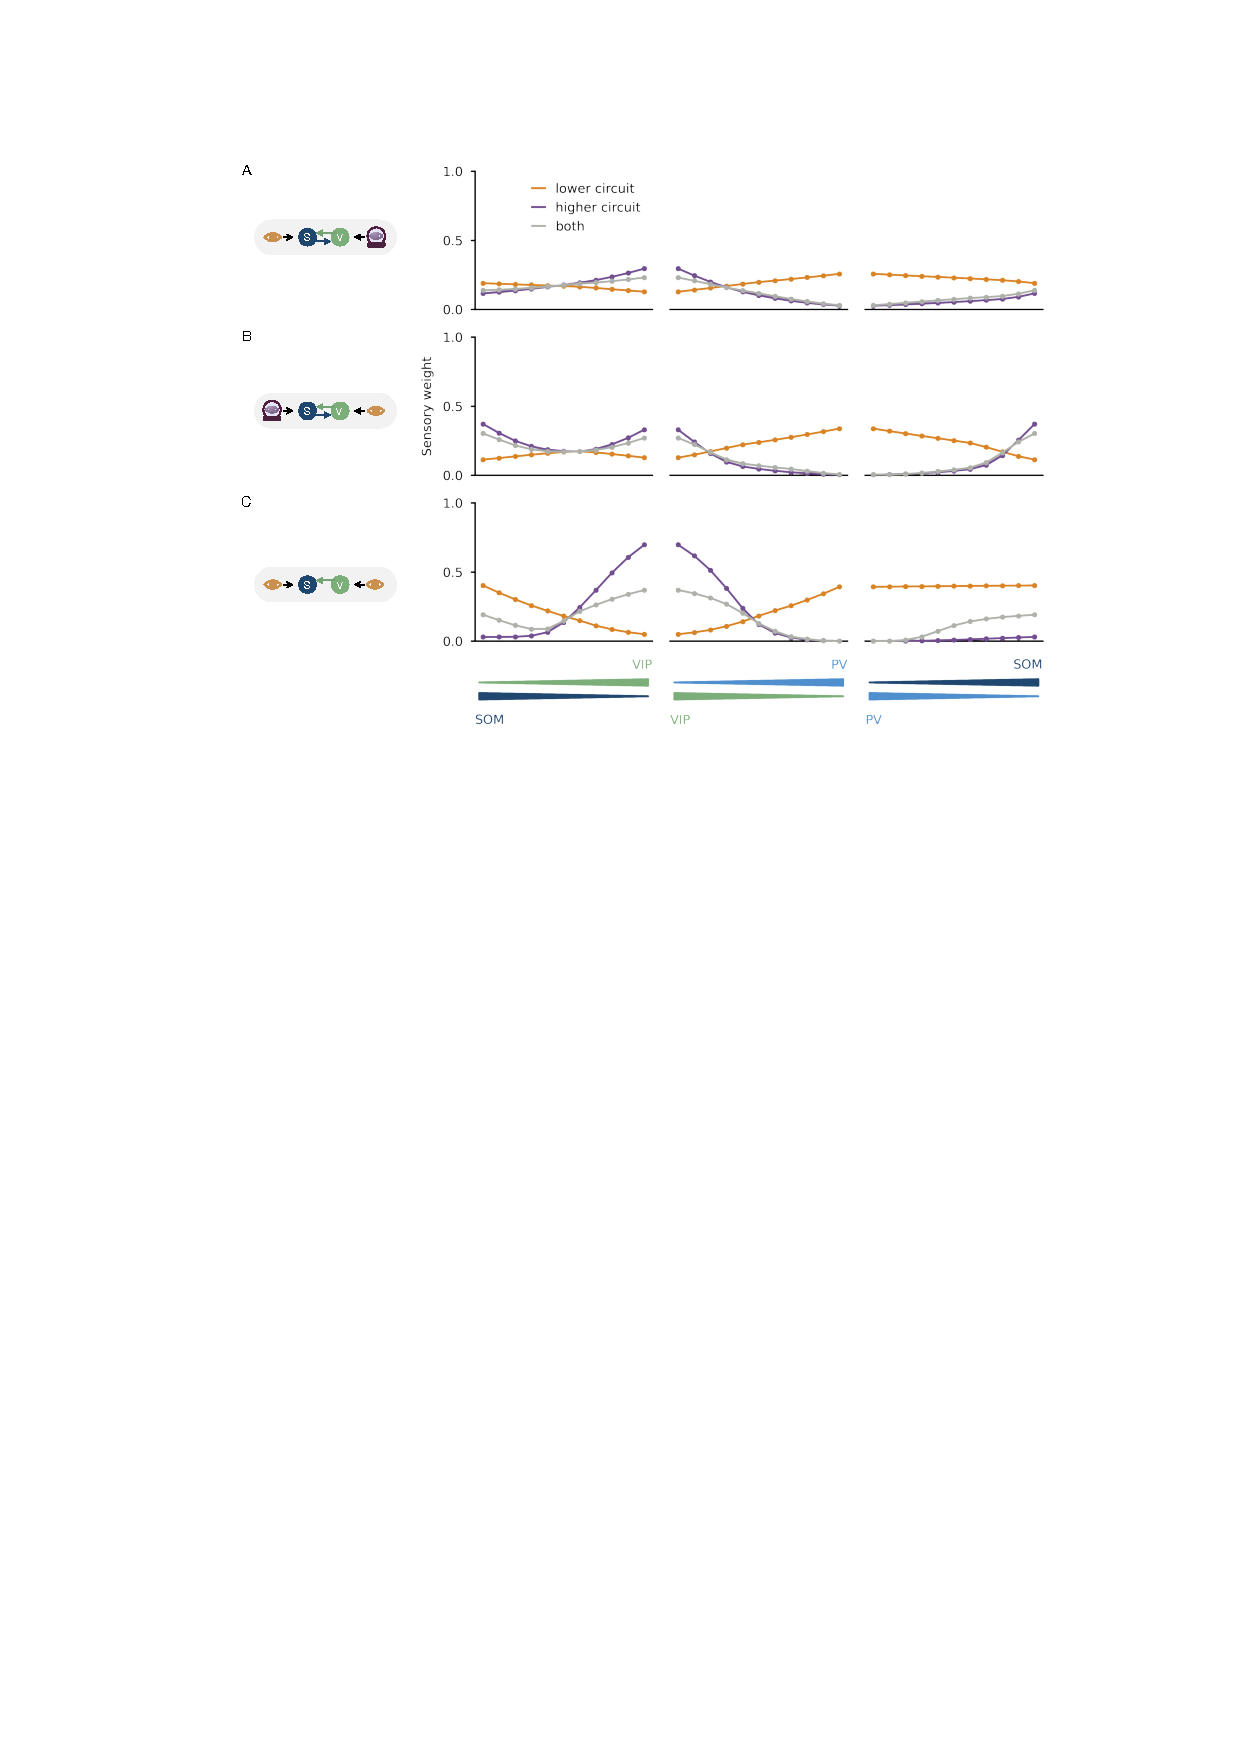
\includegraphics{../results/figures/final/Fig_4_S2}%%%
%DIF <  [width=1\linewidth]
\DIFdelendFL \DIFaddbeginFL \begin{tabular}{ |c|c|c|c| }
\hline
 & \textbf{\DIFaddFL{MFN 1}} & \textbf{\DIFaddFL{MFN 2}} & \textbf{\DIFaddFL{MFN 3}}  \\
\textbf{\DIFaddFL{Network}} & \DIFaddFL{FF $\rightarrow$ SOM  }& \DIFaddFL{FB $\rightarrow$ SOM  }& \DIFaddFL{FF $\rightarrow$ SOM  }\\
 & \DIFaddFL{FB $\rightarrow$ VIP  }& \DIFaddFL{FF $\rightarrow$ VIP  }& \DIFaddFL{FF $\rightarrow$ VIP  }\\
\hline
\hline
\DIFaddFL{nPE }& \DIFaddFL{1 }& \DIFaddFL{1.7 }& \DIFaddFL{2.5}\\
\DIFaddFL{pPE }& \DIFaddFL{1 }& \DIFaddFL{1.7 }& \DIFaddFL{2.5 }\\
\hline
\end{tabular}
\caption{\footnotesize{Gain factors for nPE and pPE neurons in three different mean-field networks (MFN). Each MFN differs with respect to the inputs onto SOM and VIP neurons. The interneurons either receive the feedforward (FF) or feedback (FB) input. All numbers are rounded to the first digit.}}
\label{tab:gain_factors_MFN}
\end{table}
%DIF > 
%DIF > 
\begin{figure}[h!]
	\centering
    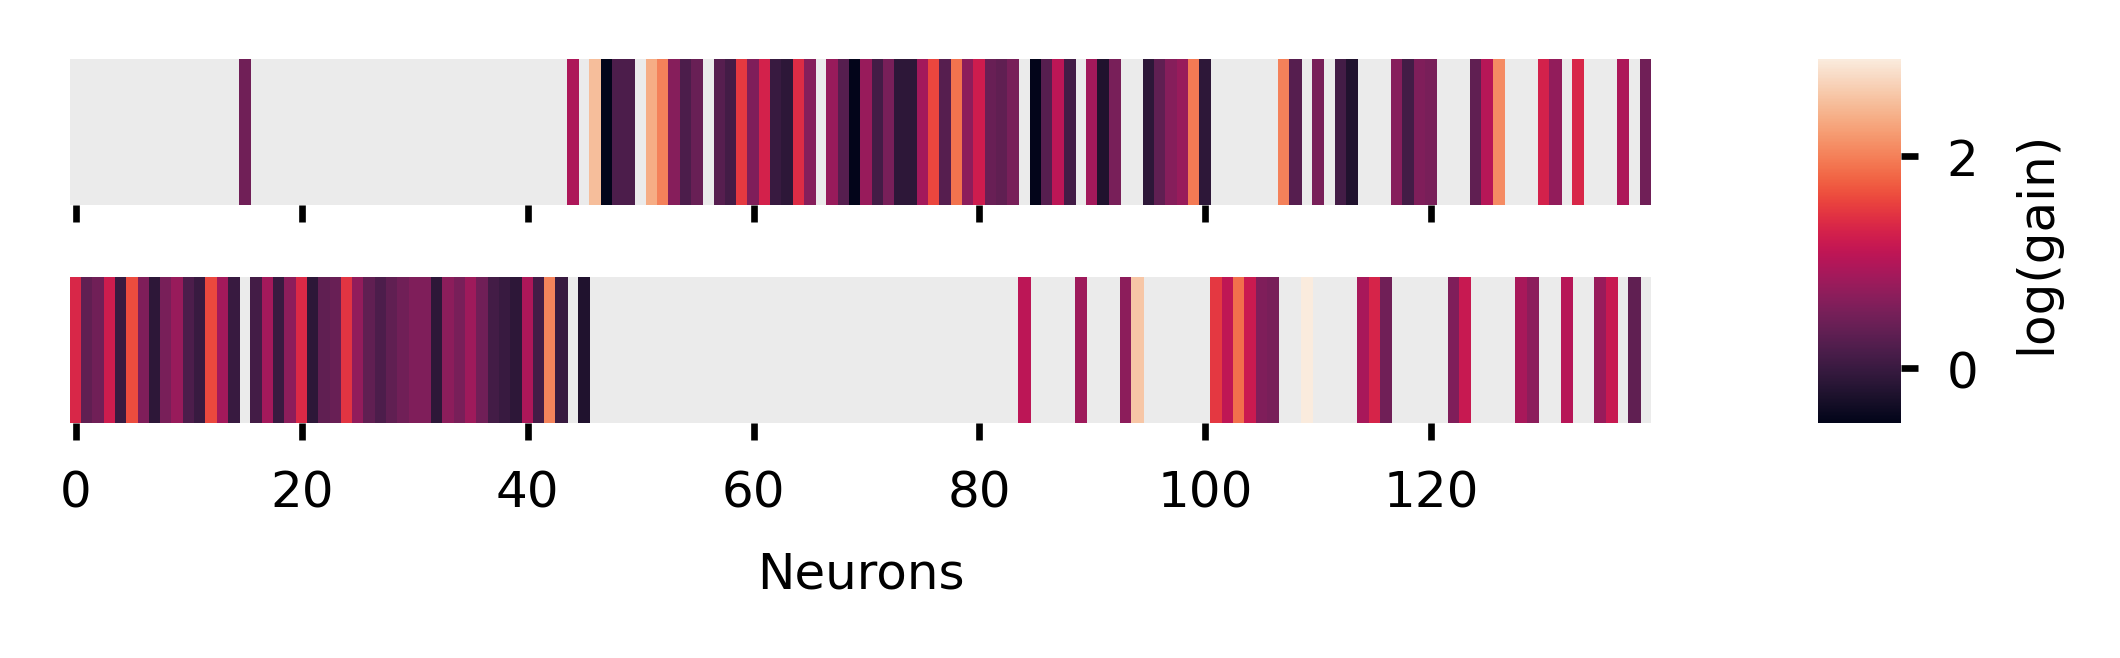
\includegraphics{../results/figures/final/Figure_gains}
\DIFaddendFL \caption{\DIFdelbeginFL %DIFDELCMD < \footnotesize{\bf Perturbing the interneurons changes the baseline and gain of nPE and pPE neurons.\newline}  
%DIFDELCMD < %%%
\DIFdelendFL \DIFaddbeginFL \footnotesize{\bf Gain factors of nPE and pPE neurons in the population model.\newline}
\DIFaddendFL {\DIFdelbeginFL %DIFDELCMD < \bf %%%
\DIFdelFL{(A)}%DIFDELCMD < } %%%
\DIFdelFL{Changes in }\DIFdelendFL \DIFaddbeginFL \DIFaddFL{The logarithm of }\DIFaddendFL the \DIFdelbeginFL \DIFdelFL{baseline activity }\DIFdelendFL \DIFaddbeginFL \DIFaddFL{gain factors }\DIFaddendFL of nPE \DIFaddbeginFL \DIFaddFL{(top) }\DIFaddendFL and pPE \DIFdelbeginFL \DIFdelFL{neurons for different interneurons targeted. 3 different mean-field networks are tested.
}%DIFDELCMD < {\bf %%%
\DIFdelendFL (\DIFdelbeginFL \DIFdelFL{B}\DIFdelendFL \DIFaddbeginFL \DIFaddFL{bottom}\DIFaddendFL ) \DIFdelbeginFL %DIFDELCMD < } %%%
\DIFdelFL{Same as }\DIFdelendFL \DIFaddbeginFL \DIFaddFL{neurons }\DIFaddendFL in \DIFdelbeginFL \DIFdelFL{(A) but for }\DIFdelendFL the \DIFdelbeginFL \DIFdelFL{gain of }\DIFdelendFL \DIFaddbeginFL \DIFaddFL{population model from \mbox{%DIFAUXCMD
\citep{hertag2022prediction}}\hskip0pt%DIFAUXCMD
. The network contains $67$ }\DIFaddendFL nPE \DIFaddbeginFL \DIFaddFL{neurons }\DIFaddendFL and \DIFaddbeginFL \DIFaddFL{$66$ }\DIFaddendFL pPE neurons. \DIFdelbeginFL \DIFdelFL{Simulation parameters}\DIFdelendFL \DIFaddbeginFL \DIFaddFL{The remaining excitatory neurons were not classified as PE neurons and were not connected to the $M$ neuron.}}}
\label{fig:Fig_gains}
\end{figure}
%DIF > 
%DIF > 

\DIFadd{The memory neuron }\textit{\DIFadd{M}} \DIFadd{connects to the post-synaptic neurons }\textit{\DIFadd{X}} \DIFadd{in the PE circuit with the connection strength $w_\mathrm{X\leftarrow M}$. If a connection exists, we assume $w_\mathrm{X\leftarrow M} = 1$. In all mean-field networks and the population network, the dendrites of nPE and pPE neurons and one of the two (populations of) PV neurons receive connections from the memory neuron. Furthermore, we assume that the }\textit{\DIFadd{M}} \DIFadd{neuron does not excite the soma of PCs. Whether the SOM or VIP neurons are the target of the feedback projections depend on the specific mean-field network (see Table \ref{tab:wXM}). In the population model, 30\% of the SOM neurons and 70\% of the VIP neurons receive input from the memory neuron.
%DIF > 
}\begin{table}[h!]
\centering
\begin{tabular}{ |c|c|c|c|  }
\hline
 & \textbf{\DIFaddFL{MFN 1}} & \textbf{\DIFaddFL{MFN 2}} & \textbf{\DIFaddFL{MFN 3}}  \\
\textbf{\DIFaddFL{Network}} & \DIFaddFL{FF $\rightarrow$ SOM  }& \DIFaddFL{FB $\rightarrow$ SOM  }& \DIFaddFL{FF $\rightarrow$ SOM  }\\
 & \DIFaddFL{FB $\rightarrow$ VIP  }& \DIFaddFL{FF $\rightarrow$ VIP  }& \DIFaddFL{FF $\rightarrow$ VIP  }\\
\hline
\hline
\DIFaddFL{SOM }& \DIFaddFL{0 }& \DIFaddFL{1 }& \DIFaddFL{0}\\
\DIFaddFL{VIP }& \DIFaddFL{1 }& \DIFaddFL{0 }& \DIFaddFL{0 }\\
\hline
\end{tabular}
\caption{\footnotesize{$w_\mathrm{X\leftarrow M}$ for the post-synaptic SOM and VIP neurons in all three mean-field networks considered.}}
\label{tab:wXM}
\end{table}
%DIF > 

\subsubsection{\DIFadd{Connections between the PE circuit and the V neuron}}
%DIF > 
\DIFadd{Both nPE and pPE neurons excite the }\textit{\DIFadd{V}} \DIFadd{neuron. To ensure that the activity of the V neuron represents the variance of the input (see Analysis in \ref{sec:gain_impact}), the weights must account for differences in the gains ($g_\mathrm{nPE}$ and $g_\mathrm{pPE}$, see Table \ref{tab:gain_factors_MFN} and Fig. \ref{fig:Fig_gains}) and numbers ($N_\mathrm{nPE}$ and $N_\mathrm{pPE}$) of the PE neurons,
%DIF > 
}\begin{align*}
\DIFadd{w_\mathrm{V\leftarrow nE}\  }&\DIFadd{=\ \frac{\theta}{g_\mathrm{nPE} \cdot N_\mathrm{nPE}} \nonumber}\\
\DIFadd{w_\mathrm{V\leftarrow pE}\  }&\DIFadd{=\ \frac{\theta}{g_\mathrm{pPE} \cdot N_\mathrm{pPE}}.
}\end{align*}
%DIF > 
\DIFadd{We introduce the factor $\theta$ to compensate for cross-terms that are the result of a quadratic activation function but are not in line with the definition of the variance. 
}

\DIFadd{In the mean-field network, $\theta = 1$ because nPE and pPE neuron activity is mutually exclusive, and, hence, the cross-term $\mathrm{nPE}\cdot\mathrm{pPE}$ would be zero (under the assumption that they have a negligible baseline activity). This is also true for the population model, in which each nPE neuron only contributes a small fraction to the overall, mean nPE, and each pPE neuron only contributes a small fraction to the overall, mean pPE. 
}

\DIFadd{However, in Supp Fig. \ref{fig:Fig_2_S3}, each mean-field network receives a stimulus $s_i$ drawn from a distribution. In this case, $\theta$ must be chosen such that deviations from the true variance can be mitigated or fully corrected. The true $\theta$ depends on the distribution at hand. In our simulations, we used a uniform distribution $U(a,b)$, in which case $\theta$ can be derived from
%DIF > 
}\begin{align}
\DIFadd{\left( \sum_{i} r_\mathrm{nE,i} + \sum_{i} r_\mathrm{pE,i}\right)^2 \overset{(i)}{=} }& \DIFadd{\left( \frac{\theta}{N}  \sum_{s_i \geq \mu}^{N/2} (s_i - \mu) + \frac{\theta}{N}  \sum_{s_i \leq \mu}^{N/2} (\mu - s_i )\right)^2 \nonumber }\\
%DIF > 
\DIFadd{=}&\DIFadd{\ \frac{\theta^2}{4} \left( \frac{2}{N} \sum_{s_i \geq \mu}^{N/2} s_i - \frac{2}{N} \sum_{s_i \leq \mu}^{N/2} s_i\right)^2\nonumber}\\
%DIF > 
\DIFadd{\overset{(ii)}{=}}&\DIFadd{\ \frac{\theta^2}{4} \left( \frac{b+\mu}{2} - \frac{\mu + a}{2} \right)^2 = \frac{(b-a)^2}{16} \cdot \theta^2,
\label{eq:theta}
}\end{align}
%DIF > 
\DIFadd{where we assumed that (i) the number of nPE and pPE neurons is equal, and (ii) this number goes to infinity. Comparing eq. (\ref{eq:theta}) with the equation for the variance of a uniform distribution, $\frac{(b-a)^2}{12}$, we get $\theta = \frac{2}{\sqrt{3}}$.
}

\subsection{\DIFadd{Inputs}}
%DIF > 
\DIFadd{Each neuron (type) receives an overall input $I_i$}\DIFaddend ,
\DIFdelbegin \DIFdel{labels}\DIFdelend %DIF > 
\DIFaddbegin \begin{align*}
\DIFadd{I_i = I_i^{BL} + w_i \cdot I_{i}^{FF}
}\end{align*}
%DIF > 
\DIFadd{where $I_{i}^{FF}$ denotes a feedforward input and $I_i^{BL}$ represents an external background input that ensures reasonable baseline firing rates in the absence of sensory inputs and predictions thereof. In the case of the mean-field network, these inputs were set such that the baseline firing rates are $r_\mathrm{pE}=r_\mathrm{pD}=r_\mathrm{nE}=r_\mathrm{nD}=0\, s^{-1}$ and $r_\mathrm{P} = r_\mathrm{S}=r_\mathrm{V}=4\, s^{-1}$. In the case of the population network, we set the external inputs of all neuron types to $5\, s^{-1}$, while the background inputs to the dendrites were computed such that the dendrites are inactive during baseline.
}

\DIFadd{The feedforward input is either the direct sensory input $s$ for the lower PE circuit, or the activity of the M neuron, $r_\mathrm{M}$, for the higher PE circuit. In general, for the three mean-field networks tested, we chose $w_i = 1 - w_\mathrm{X\leftarrow M}$  (see Table \ref{tab:wXM}). In the population network, 70\% of the SOM neurons and 30\% of the VIP neurons receive the feedforward input.
}


\subsection{\DIFadd{Simulations}}
%DIF > 
\DIFadd{All simulations were performed in customized Python code written by LH. Source code to reproduce the simulations, analyses and figures will be available after publication at }\url{https://github.com/lhertaeg/weighted_sensory_prediction}\DIFadd{. Differential equations were numerically integrated using a 2\textsuperscript{nd}-order Runge-Kutta method. Neurons were initialized with $r=0/s$. 
}

\DIFadd{The qualitative results were fairly robust to the choice of the simulation parameters and are here stated merely to ensure the reproducibility of all figures. However, we note that we made use of PE circuits that had been trained on steady state inputs \mbox{%DIFAUXCMD
\citep{hertag2022prediction}}\hskip0pt%DIFAUXCMD
. Hence, we must simulate the network long enough to ensure that the PE neurons reach their steady state. Moreover, the lower-level M neuron must evolve faster than the higher-level M neuron as indicated in Fig. \ref{fig:Fig_3_S2}. Finally, the time constant of the V neurons must be of the same magnitude as the trial duration.
}

\DIFadd{In the following, we give all figure-specific parameters not directly visible or mentioned in the figures and captions. Furthermore, to increase readability, we do not include units for the parameters. All units can be deduced from the equations above. We simulated the network in Figures \ref{fig:Fig_1} and \ref{fig:Fig_2} for $10^5$ simulation time steps. In Figure \ref{fig:Fig_2}, we presented $200$ constant values, each $500$ time steps long. In Figure \ref{fig:Fig_3} (including supporting figures) we simulated $100$ trials, while in Figures \ref{fig:Fig_4} to \ref{fig:Fig_5} (including supporting figures), we simulated $200$ trials, each $5000$ time steps long. In a trail, $10$ constant values were drawn from a normal distribution $N(\mu_\mathrm{in}, \sigma^2_\mathrm{in})$, each $500$ time steps long. The stimulus mean was drawn from an uniform distribution, $U(a, b)$, with mean $\mu_\mathrm{in}$ and variance $\sigma^2_\mathrm{trial}$.}\newline\\ 
%DIF > 
\textbf{\DIFadd{Figure 1:}} \DIFadd{Constant prediction (fixed) = $5$, input mean $\in [0,10]$, input standard deviation $0$.}\\
%DIF > 
\textbf{\DIFadd{Figure 2:}} \DIFadd{Inputs drawn from a uniform distribution. B and C: input standard deviation fixed at $4.5$ when mean is varied, input mean fixed at $4.5$ when input variance is varied.}\\
%DIF > 
\textbf{\DIFadd{Figure 2 Supplementary Fig. 1:}} \DIFadd{Inputs drawn from different distributions with mean of $5$ and variance of $4$. Number of repetitions with different seeds: 20.}\\
%DIF > 
\textbf{\DIFadd{Figure 2 Supplementary Fig. 2:}} \DIFadd{Inputs drawn from a uniform distribution with mean of $5$ and variance of $4$. Time step was $0.1$. The connections from the PE neurons to the M or V neuron were altered by a factor $\gamma$ drawn from a normal distribution. If not stated otherwise, the mean of this normal distribution was $1$ and the variance $0$, while the connection probability was $1$. Number of repetitions with different seeds: 10.}\\
%DIF > 
\textbf{\DIFadd{Figure 2 Supplementary Fig. 3:}} \DIFadd{Number of time steps were $4000$. Number of identical mean-field networks: $1000$. }\\
%DIF > 
\textbf{\DIFadd{Figure 3:}} \DIFadd{C: $\sigma^2_\mathrm{in} = 0$ and $U(1,9)$, D:  $\sigma^2_\mathrm{in} = 5$ and $U(5,5)$, F: $\sigma^2_\mathrm{in} = 0$ and $U(a,b)$ was parameterized such that the trail variability was $3$.}\\
%DIF > 
\textbf{\DIFadd{Figure 3 Supplementary Fig. 1:}}  \DIFadd{Switch of input statistics occurs after 50 trails. State 1: stimulus $\in N(\mu_\mathrm{in}, 0)$ with $\mu_\mathrm{in} \in U(5,5)$, State 2:  stimulus $\in N(\mu_\mathrm{in}, 3)$ with $\mu_\mathrm{in} \in U(5,5)$, State 3: stimulus $\in N(\mu_\mathrm{in}, 3)$ with $\mu_\mathrm{in} \in U(0,10)$, State 4: stimulus $\in N(\mu_\mathrm{in}, 0)$ with $\mu_\mathrm{in} \in U(0,10)$.}\\
%DIF > 
\textbf{\DIFadd{Figure 3 Supplementary Fig. 2:}} \DIFadd{$\mu_\mathrm{in} = 5$ and $\sigma^2_\mathrm{trial} \in \lbrace0, 0.75, 1.5, 2.25, 3\rbrace$}\DIFaddend , \DIFaddbegin \DIFadd{$\sigma^2_\mathrm{in} \in \lbrace 3, 2.25, 1.5,0.75, 0\rbrace$. A: scaling factors of $w_\mathrm{M\leftarrow PE}$ were 0.3 }\DIFaddend and \DIFdelbegin \DIFdel{colors as in Fig}\DIFdelend \DIFaddbegin \DIFadd{7.}\\
%DIF > 
\textbf{\DIFadd{Figure 4:}} \DIFadd{$\mu_\mathrm{in} = 5$. A, top: $\sigma^2_\mathrm{in} = 0$ and $\sigma^2_\mathrm{trial} = 1$. A, bottom: $\sigma^2_\mathrm{in} = 1$ and $\sigma^2_\mathrm{trial} = 0$. C: $\sigma^2_\mathrm{in} = 1$ and $\sigma^2_\mathrm{trial} = 1$. D: $\sigma^2_\mathrm{in} = 5$ and $\sigma^2_\mathrm{trial} = 0$. Additional input (perturbation) was either fixed at $0.5$ (A, D) or systematically varied between $-1$ and $1$ (C), and was }\textit{\DIFadd{on}} \DIFadd{for the last 50\% of the trials. To estimate changes in baseline and gain of nPE and pPE neurons, we fitted a linear function to the PE neuron activity for the input range $[0, 2.5]$}\DIFaddend .\DIFdelbegin \DIFdel{\ref{fig:Fig_4}}\DIFdelend \DIFaddbegin \\
%DIF > 
\textbf{\DIFadd{Figure 4 Supplementary Fig. 1:}} \DIFadd{All parameters are from Figure 4 A.}\\
%DIF > 
\textbf{\DIFadd{Figure 4 Supplementary Fig. 2:}} \DIFadd{In the default setting baseline was $0$ and gain of PE neurons was $1$. The results (left) were computed for baselines $\in [0, 3]$, while the results (right) were computed for gains $\in [0.5, 1.5]$. The results are based on the Eqs. (\ref{eq:prediction_gain}), (\ref{eq:variance_gain}), (\ref{eq:condition_baseline_mean_1}) and  (\ref{eq:condition_baseline_variance_2}). }\\
%DIF > 
\textbf{\DIFadd{Figure 4 Supplementary Fig. 3:}} \DIFadd{All parameters are from Figure 4 D.}\\
%DIF > 
\textbf{\DIFadd{Figure 5:}} \DIFadd{A: $\sigma_\mathrm{in} \in \lbrace1,7\rbrace$, $\mu_\mathrm{in} \in U(15, 25)$. B: $\sigma_\mathrm{in} \in [0,8]$, $\mu_\mathrm{in} \in U(15, 25)$, and $\sigma_\mathrm{in} = 5$, $\mu_\mathrm{in} \in U(15, b)$ with $b\in [20, 48]$. C: $\sigma_\mathrm{in} \in \lbrace2,5\rbrace$, $\mu_\mathrm{in} \in U(15, 15)$. D: $\sigma_\mathrm{in} = 0$, $\mu_\mathrm{in} \in U(15, 25)$ or $U(10, 30)$. E: $\sigma_\mathrm{in} = 0$, $\mu_\mathrm{in} \in U(15, 25)$, or $\sigma_\mathrm{in} = 5$, $\mu_\mathrm{in} \in U(15, 15)$,  Time steps per trail increased from $5000$ to $10^4$}\DIFaddend .\DIFdelbegin %DIFDELCMD < \MBLOCKRIGHTBRACE
%DIFDELCMD < \label{fig:Fig_4_S2}
%DIFDELCMD < \end{figure}
%DIFDELCMD < %%%
\DIFdelend \DIFaddbegin \\
%DIF > 
\textbf{\DIFadd{Figure 5 Supplementary Fig. 1:}} \DIFadd{We used two different uniform distributions $U(15, 25)$ and  $U(25, 35)$, and introduced scalar variability so that $\sigma_\mathrm{in}$ is a linear function of $\mu_\mathrm{in}$. Specifically, we chose $\sigma_\mathrm{in} = \left[\mu_\mathrm{in} -14\right]_+$.
}\DIFaddend 


%DIF <  To continue, please "uncomment" the entire part below.
\DIFaddbegin \section{\DIFadd{Supporting analyses}}
\DIFaddend 

%DIF < \section*{Discussion}
\DIFaddbegin \DIFadd{We first describe a simplified model and show that the M neuron represents the mean, while the V neuron represents the variance of the feedforward input. We then investigate the impact of the gain and baseline of PE neurons on estimating the mean and variance. Furthermore, we use the simplified model to discuss the effect of neuromodulators in our network. Finally, we reveal the connection between the sensory weight and the contraction bias.
}

\subsection{\DIFadd{Activity of M and V neuron in a simplified model}}\label{sec:toy}
\DIFaddend %
%DIF < We solved the brain.
\DIFaddbegin \DIFadd{To show that the M neuron encodes the mean, while the V neuron encodes the variance of the feedforward input, we resume a toy model in which the activity of the nPE and pPE neuron is replaced by its ideal output
}\DIFaddend %
%DIF < % At the end, or in between talk about changes in PE neurons directly that you have currently in Fig. 3 SX ... I copy the part of the last paragraph here as inspiration :
%DIF < % For some psychiatric disorders, it has been shown that the weighting of sensory inputs and predictions thereof is impaired (XXX), leading to an overweighting of one of these signals. Moreover, it has been hypothesised that factors like stress or cognitive load may also influence the processing of feedforward and feedback inputs (XXX). ... Another factor that may contribute to a distorted weighting is the baseline activity of PE neurons that was set to zero in our model, in line with very low spontaneous firing rates of excitatory neurons in rodent primary sensory areas (XXX). Increasing this baseline activity for the nPE neuron (Fig. SXXX), pPE neuron (Fig. SXXX) or both pushes the network to weight sensory stimuli and predictions more equally. We speculate that an increase of baseline activity may be a natural result of an increased cognitive load or stress. 
\DIFaddbegin \begin{align}
\DIFadd{r_\mathrm{nE} = \left[ r_\mathrm{M} - s_\mathrm{FF}\right]_+ \nonumber }\\
\DIFadd{r_\mathrm{pE} = \left[ s_\mathrm{FF} - r_\mathrm{M} \right]_+
}\end{align}
\DIFaddend %
%DIF < % mention Pakan paper
\DIFaddbegin \DIFadd{with $s_\mathrm{FF}$ denoting the time-dependent feedforward input. The activity of the M neuron can then be described as
}\DIFaddend %
%DIF < \section*{Models and methods}
%DIF < %
\DIFaddbegin \begin{align}
\DIFadd{\tau_M \cdot \frac{dr_\mathrm{M}}{dt} = r_\mathrm{pE} - r_\mathrm{nE}
}\end{align}
\DIFaddend %
%DIF < \subsection*{Network model}
%DIF < %
%DIF < Network consists of two subnetworks. Each subnetwork consists of a PE circuit, a memory neuron and a neuron representing the variance. XXX The memory neuron of subnetwork feefdowradly connects to the PE circuit of the second subnetwork.
\DIFaddbegin \DIFadd{If $r_\mathrm{M} \geq s_\mathrm{FF}$, we get
}\DIFaddend %
%DIF < \subsubsection*{Prediction-error network model}
%DIF < %
%DIF < Consider a mean field network in which each population is represented by one representative neuron. The mean-field PE network consists of an excitatory nPE and pPE neuron, as well as two inhibitory PV neurons (one receiving S, the other P), as well as inhibitory SOM and VIP neurons.
\DIFaddbegin \begin{align}
\DIFadd{\tau_M \cdot \frac{dr_\mathrm{M}}{dt} = -r_\mathrm{nE} = -r_\mathrm{M} + s_\mathrm{FF}.
}\end{align}
\DIFaddend %
%DIF < Each excitatory pyramidal cell (that is, nPE or pPE neuron) is divided into two coupled compartments, representing the soma and the dendrites, respectively. The dynamics of the firing rate~$r_{\mathrm{E}}$ of the somatic compartment of obeys \citep{wilson1972excitatory}
%DIF < %
%DIF < \begin{align}
%DIF < \tau_E\ \frac{dr_\mathrm{E}}{dt} &= - r_\mathrm{E} + w_\mathrm{ED}\cdot  r_\mathrm{D}  -  w_\mathrm{EP}\cdot r_\mathrm{P} + I_\mathrm{E},
%DIF < \end{align}
%DIF < %
%DIF < where $\tau_\mathrm{E}$ denotes the excitatory rate time constant ($\tau_\mathrm{E}$=60 ms), the weight $w_{\mathrm{ED}}$ describes the connection strength between the dendritic compartment and the soma of the same neuron, and $w_{\mathrm{EP}}$ denotes the strength of somatic inhibition from PV neurons. The overall input $I_\mathrm{E}$ comprises external background and feedforward sensory  inputs (see ``Inputs" below). Firing rates are rectified to ensure positivity.
\DIFaddbegin \DIFadd{If $r_\mathrm{M} \leq s_\mathrm{FF}$, we also get
}\DIFaddend %
%DIF < The dynamics of the activity~$r_\mathrm{D}$ of the dendritic compartment obeys \citep{wilson1972excitatory}
%DIF < %
%DIF < \begin{align}
%DIF < \tau_E\ \frac{dr_\mathrm{D}}{dt} &= - r_\mathrm{D} +  w_\mathrm{DE}\cdot r_\mathrm{E}  - w_\mathrm{DS}\cdot r_\mathrm{S} + I_\mathrm{D},
%DIF < \end{align}
%DIF < %
%DIF < where the weight $w_{\mathrm{DE}}$ denotes the recurrent excitatory connections between PCs, including backpropagating activity from the soma to the dendrites. $w_{\mathrm{DS}}$ represents the strength of dendritic inhibition from SOM neurons. The overall input $I_\mathrm{D}$ comprises fixed, external background inputs and feedback predictions (see ``Inputs" below). We assume that any excess of inhibition in a dendrite does not affect the soma, that is, the dendritic compartment is rectified at zero. 
\DIFaddbegin \begin{align}
\DIFadd{\tau_M \cdot \frac{dr_\mathrm{M}}{dt} = r_\mathrm{pE} = -r_\mathrm{M} + s_\mathrm{FF}.\nonumber
}\end{align}
\DIFaddend %
%DIF < Just as for the excitatory neurons, the firing rate dynamics of each interneuron is modeled by a rectified, linear differential equation \citep{wilson1972excitatory},
%DIF < %
%DIF < \begin{align}
%DIF < \label{eq:RateEqINs}
%DIF < \tau_I\ \frac{dr_\mathrm{X}}{dt} =& - r_\mathrm{X} + I_{\mathrm{X}} + w_\mathrm{XE}\cdot r_\mathrm{E} - w_\mathrm{XP}\cdot r_\mathrm{P}  - w_\mathrm{XS}\cdot r_\mathrm{S} -  w_\mathrm{XV}\cdot r_\mathrm{V}, 
%DIF < \end{align}
%DIF < %
%DIF < where $r_\mathrm{X}$ denotes the firing rate of neuron type $X$, and the weight matrices $w_\mathrm{XY}$ denote the strength of connection between the presynaptic neuron population $Y$ and the postsynaptic neuron population $X$ ($X, Y\in \lbrace P,S,V\rbrace$). The rate time constant $\tau_I$ was chosen to resemble a fast GABA\textsubscript{A} time constant, and set to 2 ms for all interneuron types included. The overall input $I_\mathrm{X}$ comprises fixed, external background inputs, as well as feedforward sensory inputs and feedback predictions (see ``Inputs" below).
\DIFaddbegin \DIFadd{Hence, the activity of $r_\mathrm{M}$ is given by
}\DIFaddend %
%DIF < \subsubsection*{Memory and variance neuron}
%DIF < %
%DIF < \begin{align}
%DIF < \tau_m \cdot \frac{dr_\mathrm{M}}{dt} = w_\mathrm{M\leftarrow pPE} \cdot r_\mathrm{pPE} - w_\mathrm{M\leftarrow nPE} \cdot r_\mathrm{nPE} 
%DIF < \end{align}
%DIF < %
%DIF < \begin{align}
%DIF < \tau_v \cdot \frac{dr_\mathrm{V}}{dt} = -r_\mathrm{V} + (w_\mathrm{V\leftarrow pPE} \cdot r_\mathrm{pPE} - w_\mathrm{V\leftarrow nPE} \cdot r_\mathrm{nPE})^2 
%DIF < \end{align}
\DIFaddbegin \begin{align}
\DIFadd{r_\mathrm{M} = \frac{1}{\tau_M} \int\limits_0^t e^{-(t-x)/\tau_M}\cdot s_\mathrm{FF}(x)\ dx
}\end{align}  
\DIFaddend %
%DIF < \subsubsection*{Weighted output}
%DIF < %
%DIF < \begin{align}
%DIF < r_\mathrm{out} = \alpha \cdot S + (1-\alpha) \cdot P
%DIF < \end{align}
%DIF < %
%DIF < \begin{align}
%DIF < \alpha &= \frac{1/r_\mathrm{V1}}{1/r_\mathrm{V1} + 1/r_\mathrm{V2}}\nonumber\\
%DIF < & = \left( 1 + \frac{r_\mathrm{V1}}{r_\mathrm{V2}} \right)^{-1}
%DIF < \end{align}
\DIFaddbegin \DIFadd{for zero activity at time $t=0$. In the limit of $t\rightarrow \infty$ (steady state), this is exactly the exponential average of the feedforward input, $E(s_\mathrm{FF})$.
}

\DIFadd{With the simplified activity of the nPE and pPE neuron, the activity of the V neuron can then be described as
}\DIFaddend %
%DIF < \subsection*{Connectivity}
%DIF < %
%DIF < %All neurons are randomly connected with connection probabilities motivated by the experimental literature \citep[e.g.][]{fino2011dense, packer2011dense, pfeffer2013inhibition, lee2013disinhibitory, pi2013cortical, jiang2015principles, jouhanneau2015vivo, pala2015vivo},
%DIF < %%
%DIF < %\begin{align}
%DIF < %p = \begin{pmatrix}
%DIF < %  p_\mathrm{EE}  & p_\mathrm{ED} & p_\mathrm{EP} & p_\mathrm{ES} & p_\mathrm{EV} \\
%DIF < %  p_\mathrm{DE}  & p_\mathrm{DD} & p_\mathrm{DP} & p_\mathrm{DS} & p_\mathrm{DV} \\
%DIF < %  p_\mathrm{PE}  & p_\mathrm{PD} & p_\mathrm{PP} & p_\mathrm{PS} & p_\mathrm{PV} \\
%DIF < %  p_\mathrm{SE}  & p_\mathrm{SD} & p_\mathrm{SP} & p_\mathrm{SS} & p_\mathrm{SV} \\
%DIF < %   p_\mathrm{VE} & p_\mathrm{VD} & p_\mathrm{VP} & p_\mathrm{VS} & p_\mathrm{VV} \\
%DIF < %\end{pmatrix}
%DIF < %=
%DIF < %\begin{pmatrix}
%DIF < %  - & 1 & 0.6 & - & -\\
%DIF < %  0.1  & - & - & 0.55 & - \\
%DIF < %  0.45  & - & 0.5 & 0.6 & 0.5 \\
%DIF < %  0.35  & - & - & - & 0.5 \\
%DIF < %   0.1 & - & - & 0.45 & - \\
%DIF < %\end{pmatrix}.
%DIF < %\label{Mtx:ConnProb}
%DIF < %\end{align}
%DIF < %%
%DIF < %All cells of the same neuron type have the same number of incoming connections. The mean total connection strengths are set to
%DIF < %%
%DIF < %\begin{align}
%DIF < %w = \begin{pmatrix}
%DIF < %  w_\mathrm{EE}  & w_\mathrm{ED} & w_\mathrm{EP} & w_\mathrm{ES} & w_\mathrm{EV} \\
%DIF < %  w_\mathrm{DE}  & w_\mathrm{DD} & w_\mathrm{DP} & w_\mathrm{DS} & w_\mathrm{DV} \\
%DIF < %  w_\mathrm{PE}  & w_\mathrm{PD} & w_\mathrm{PP} & w_\mathrm{PS} & w_\mathrm{PV} \\
%DIF < %  w_\mathrm{SE}  & w_\mathrm{SD} & w_\mathrm{SP} & w_\mathrm{SS} & w_\mathrm{SV} \\
%DIF < %   w_\mathrm{VE} & w_\mathrm{VD} & w_\mathrm{VP} & w_\mathrm{VS} & w_\mathrm{VV} \\
%DIF < %\end{pmatrix}
%DIF < %=
%DIF < %\begin{pmatrix}
%DIF < %  - & 1 & 2^{*} & - & -\\
%DIF < %  0.5 & - & - & 0.5^{*} & -\\
%DIF < %  1.2 & - & 1 & 0.3^{*} & 0.3^{*} \\
%DIF < %  1 & - & - & - & 0.6 \\
%DIF < %  1 & - & - & 0.7 & - \\
%DIF < %\end{pmatrix},
%DIF < %\label{Mtx:ConnStrengths}
%DIF < %\end{align}
%DIF < %%
%DIF < %where $^{*}$ denotes either the weights that are free for optimization to satisfy the equations describing an E/I balance (see Supporting Information), or the initial mean connection strengths that are subject to synaptic plasticity during learning. For plastic networks, the initial connections between neurons are drawn from uniform distributions 
%DIF < %%
%DIF < %\begin{align*}
%DIF < %w_{ij}^{initial} \in \mathcal{U} \left(0.5\ w, 1.5\ w\right),
%DIF < %\end{align*}
%DIF < %%
%DIF < %where $w$ denotes the mean connection strengths given in (\ref{Mtx:ConnStrengths}). Please note that the system is robust to the choice of connection strengths. The connection strengths are merely chosen such that the solutions of the equations describing an E/I balance comply with Dale's principle.
%DIF < %
%DIF < %In plastic networks, $w_\mathrm{EP}$ is subdivided into assemblies. While one-third of PCs receive stronger initial inhibition from PV neurons that are driven by sensory input, another third receives stronger initial inhibition from PV neurons that are driven by feedback predictions. More precisely, for two-thirds of the excitatory neurons, half of the connections from PV neurons are strengthened by $1.5$, while the remaining ones are weakened by $0.5$.
%DIF < %
%DIF < %All weights are scaled in proportion to the number of existing connections (i.e., the product of the number of presynaptic neurons and the connection probability), so that the results are independent of the population size.
\DIFaddbegin \begin{align}
\DIFadd{\tau_V \cdot \frac{dr_\mathrm{V}}{dt} = -r_\mathrm{V} + (r_\mathrm{pE} +  r_\mathrm{nE})^2 = -r_\mathrm{V}  + (r_\mathrm{M} -  s_\mathrm{FF})^2,
}\end{align}
\DIFaddend %
%DIF < \subsection*{Inputs}
%DIF < %
%DIF < %All neurons receive external background input that ensures reasonable baseline firing rates in the absence of sensory inputs and predictions thereof. In the case of non-plastic networks, these inputs were set such that the baseline firing rates are $r_\mathrm{E}=1\, s^{-1}$, $r_\mathrm{P} = r_\mathrm{S}=r_\mathrm{V}=4\, s^{-1}$ and $r_\mathrm{D}=0\, s^{-1}$. In the case of plastic networks, we set the external inputs of all neuron types to $x_\mathrm{E}=x_\mathrm{P}=x_\mathrm{S}=x_\mathrm{V}=5\, s^{-1}$, while the background input to the dendrites is dynamically computed during training such that $r_\mathrm{D}=0\, s^{-1}$.
%DIF < %
%DIF < %In addition to the external background inputs, the neurons receive either sensory input~($S$), a prediction thereof ($P$), or both. We distinguish between phases of fully predicted ($P=S>0$), overpredicted ($P>S$) and underpredicted ($P<S$) sensory stimuli, as well as baseline phases ($P=S=0$). During training, the network is exposed to baseline phases and fully predicted sensory inputs (Figs.~\ref{fig:Fig_Plasticity} and \ref{fig:Fig_Experience}), or in addition to over- and underpredicted sensory stimuli (Fig.~\ref{figsupp:Fig_Experience_Predictability}). Stimuli are drawn from a uniform distribution from the interval $[0, 5\, s^{-1}]$. Mean and SD of test stimuli for each simulation are listed below (see ``Simulations").
\DIFaddbegin \DIFadd{leading to the time-dependent solution
}\DIFaddend %
\DIFaddbegin \begin{align}
\DIFadd{r_\mathrm{V} = \frac{1}{\tau_V} \int\limits_0^t e^{-(t-x)/\tau_V}\cdot \left[r_\mathrm{M}(x) -  s_\mathrm{FF}(x)\right]^2\ dx.
}\end{align}  
\DIFaddend %
%DIF < \subsection*{Simulations}
%DIF < %
%DIF < %All simulations were performed in customized Python code written by LH. Differential equations were numerically integrated using a 2\textsuperscript{nd}-order Runge-Kutta method with time steps ranging between $0.1$ and $0.2$ ms. Neurons in the PE circuits were initialized with $r=0/s$. The memory neurons were initialized at the mean of the two distributions (see above), and each prediction neuron was either set to the mean of the distribution it is associated with if the stimulus at $t=0\ \mathrm{ms}$ was drawn from that distribution, or set to zero otherwise. Each stimulus was presented for $1$ second. During training of the PE circuit, we presented 350 stimuli alternated with 350 zero-input (baseline) phases. We made sure that the weights converged to a configuration that satisfied the objective given by our homeostatic plasticity rules (see Eqs.~\ref{eq:Plasticity_I}-\ref{eq:Plasticity_II} in ``Plasticity model"). We defined the steady-state firing rate per stimulus as the activity in the last 500 ms of stimulus presentation. The onset firing rate was computed as the activity of the first 10 ms.\\\\
%DIF < %%
%DIF < %\textbf{Figures 1 \& S2:} Test stimulus was set to $5/s$ with a SD of $1/s$. Stimulus to compute total excitatory and inhibitory inputs was set to $1/s$.\\
%DIF < %%
%DIF < %\textbf{Figures 2 \& S3:} Test stimulus was set to $3/s$ with a SD of $1/s$. The perturbation stimuli ranged from $-1.5/s$ to $1.5/s$.\\
%DIF < %%
%DIF < %\textbf{Figures 3, S4 \& S5:} Test stimulus was set to $5/s$ with a SD of $1.5/s$. 50\% of the PV neurons, 70\% of the SOM neurons and 30\% of the VIP neurons receive the actual sensory input, while the remaining ones of each population received a prediction thereof. Perturbation stimulus was $\pm 2/s$. Panels D \& G of Fig. 3 show the median over all PE neurons and the SEM.\\
%DIF < %%
%DIF < %\textbf{Figures 4 \& S6:} Test stimulus was set to $5/s$ with a SD of $1.5/s$. In main figure, square: $w_\mathrm{EP}\in[2,4]$, $w_\mathrm{PS}\in[0.5,1]$, $w_\mathrm{PV}\in[1.5,2.5]$; circle: $w_\mathrm{EP}\in[2.5,8]$, $w_\mathrm{PS}\in[1.5,2.5]$, $w_\mathrm{PV}\in[0.5,1]$; triangle: $w_\mathrm{EP}\in[2.5,8]$, $w_\mathrm{PS}\in[1,2.5]$, $w_\mathrm{PV}\in[0.5,2]$. Half of the PV neurons and all SOM neurons receive the actual sensory input, while the remaining PV and SOM neurons as well as all VIP neurons receive a prediction thereof.
%DIF < %In supporting figure: Total number of stimuli presented during training was increased, so that the number of fully predicted sensory stimuli was constant at 350. Results were averaged over 5 simulations, mean and SD are shown.\\
%DIF < %%
%DIF < %\textbf{Figure 5:} For panel E, the performance error was computed as the squared difference between the activity of the respective line attractor and the stimulus presented. For panel F, the initial weight between the stimulus and the representation neuron was set to $0.5$. The basis learning rate (fixed) was set to $5e^{-4}$. And the initial speed was computed as the derivative of the rate with respect to time, averaged over the first 50 ms. 
%DIF < %
%DIF < %Source code to reproduce the simulations, analyses and figures will be available after publication at \url{github.com/lhertaeg/SourceCode_Hertaeg2021}. 
\DIFaddbegin \DIFadd{In the limit of $t\rightarrow \infty$, $r_\mathrm{V}$ approaches $E(s_\mathrm{FF} - E(s_\mathrm{FF}))$.
}


\subsection{\DIFadd{Impact of PE neurons' gain on estimating mean and variance}}\label{sec:impact_gain}\label{sec:gain_impact}
\DIFaddend %
%DIF < \section*{Acknowledgments}
%DIF < %
%DIF < %We are grateful to Vezha Boboeva, Douglas Feitosa Tom\'e, J\'ulia Gallinaro and Klara Kaleb for helpful comments on earlier versions of this manuscript, and we want to thank all members of the Clopath lab for discussion and support. This work was supported by BBSRC BB/N013956/1, BB/N019008/1, Wellcome Trust 200790/Z/16/Z, Simons Foundation 564408 and EPSRC EP/R035806/1.
\DIFaddbegin \DIFadd{The gains of the PE neurons, if not equal between nPE and pPE neuron on average, can bias the activity of both the M and V neuron. To show this, we resume the toy model from section \ref{sec:toy}. 
}\DIFaddend %
%DIF < \bibliographystyle{naturemag} %{plainnat}
%DIF < \bibliography{../References_Mismatch}
\DIFaddbegin \begin{align}
\DIFadd{\label{eq:condition_mean_gain_equal}
g_\mathrm{pPE}\ \langle r_\mathrm{nPE}\rangle }&\DIFadd{= g_\mathrm{nPE}\ \langle r_\mathrm{pPE}\rangle }\\
\DIFadd{g_\mathrm{pPE}\ \langle \left[ s_\mathrm{FF}-P\right]_+\rangle }&\DIFadd{= g_\mathrm{nPE}\ \langle \left[ P-s_\mathrm{FF}\right]_+\rangle \nonumber}\\
\DIFadd{g_\mathrm{pPE} \int\limits_P^{\infty} \left( x-P\right)\ f(x)\ dx }&\DIFadd{= g_\mathrm{nPE} \int\limits_{-\infty}^P \left( P-x\right)\ f(x)\ dx. \nonumber
}\end{align}
\DIFaddend %
\DIFaddbegin \DIFadd{Here, $P$ denotes the prediction encoded in the M neuron, and $f(x)$ is the distribution of feedforward inputs. In case of a uniform distribution, $f(x) = 1/(b-a)$ for $x\in [a,b]$ and $0$ otherwise, we get
}\DIFaddend %
\DIFaddbegin \begin{equation}
\DIFadd{\label{eq:prediction_gain}
    P=
    \begin{cases}
      \frac{a + b}{2} & \text{if}\ g_\mathrm{nPE} = g_\mathrm{pPE} = g \\
      \frac{g_\mathrm{pPE}\cdot b - g_\mathrm{nPE}\cdot a + \sqrt{g_\mathrm{nPE}\ g_\mathrm{pPE}}\ (a-b)}{g_\mathrm{pPE} - g_\mathrm{nPE}} & \text{otherwise.}
    \end{cases}
}\end{equation}
\DIFaddend %
%DIF < %%%%%%%%%%%%%%%%%%%%%%%%%%%%%%%%%%%%%%%%%%%%%%%%%%%%%%%%%%%%
%DIF < %%% APPENDICES
%DIF < %%%%%%%%%%%%%%%%%%%%%%%%%%%%%%%%%%%%%%%%%%%%%%%%%%%%%%%%%%%%
\DIFaddbegin \DIFadd{Hence, the mean of the feedforward input is overpredicted when $g_\mathrm{nPE} < g_\mathrm{pPE}$. Similarly, the mean of the feedforward input is underpredicted when $g_\mathrm{nPE} > g_\mathrm{pPE}$ (Fig. \ref{fig:Fig_4_S2}).
}

\DIFadd{Likewise, the variance is affected by the gain of the nPE and pPE neuron,
}\DIFaddend %
\DIFaddbegin \begin{align}
\DIFadd{\label{eq:condition_variance_gain}
V }&\DIFadd{= \langle \left(r_\mathrm{pPE} + r_\mathrm{nPE}\right)^2 \rangle \overset{(i)}{=} \langle r_\mathrm{pPE}^2 \rangle + \langle r_\mathrm{nPE}^2 \rangle \nonumber}\\
&\DIFadd{=g_\mathrm{pPE}^2\ \langle \left[ s_\mathrm{FF}-P \right]_+^2 \rangle + g_\mathrm{nPE}^2\ \langle \left[ P-s_\mathrm{FF} \right]_+^2 \rangle,
}\end{align}
\DIFaddend %
%DIF < \newpage
%DIF < \section*{Supplementary Information}
%DIF < \appendix
\DIFaddbegin \DIFadd{where we assume (i) that both the nPE and pPE neuron have a zero baseline activity. In case of a uniform distribution, we get
}\DIFaddend %
\DIFaddbegin \begin{align}
\DIFadd{V }&\DIFadd{= \frac{g_\mathrm{pPE}^2}{b-a} \int\limits_P^b (x-P)^2\ dx + \frac{g_\mathrm{nPE}^2}{b-a} \int\limits_a^P (P-x)^2\ dx }\\
   &\DIFadd{= \frac{g_\mathrm{pPE}^2}{3} \cdot \frac{(b-P)^3}{b-a} + \frac{g_\mathrm{nPE}^2}{3} \cdot \frac{(P-a)^3}{b-a}. \nonumber
}\end{align}
\DIFaddend %
%DIF < \subsection*{Sensory weight and contraction bias}
%DIF < %
%DIF < If P is rather constant, the slope in the contraction bias is exactly the sensory weight
%DIF < %
%DIF <  \begin{align*}
%DIF <  r_\mathrm{out} = \alpha_\mathrm{S} \cdot S + \left( 1 -\alpha_\mathrm{S} \right) \cdot P \equiv m \cdot S + n
%DIF <  \end{align*}
%DIF < %
%DIF < However, P is usually/normally a function of $S$. For simplicity, let's assume that P decays exponentially to a new value of $S$:
%DIF < %
%DIF < \begin{align*}
%DIF < P = P_\mathrm{0} \cdot \mathrm{e}^{-t/\tau} + f(S) \cdot \left( 1 -   \mathrm{e}^{-t/\tau} \right)
%DIF < \end{align*}
%DIF < %
%DIF < Within each trial with trial duration T, P can be expressed by n sections of length t in which the stimulus is constant and, for the sake of simplicity, drawn from a uniform distribution $U\left( s - \frac{\sigma_\mathrm{S}}{12}, s + \frac{\sigma_\mathrm{S}}{12} \right)$. $P_\mathrm{0}$ is drawn from $U\left( \mu - \frac{\sigma_\mathrm{P}}{12}, \mu + \frac{\sigma_\mathrm{P}}{12} \right)$. $P_\mathrm{n}$ is then given by
%DIF < %
%DIF < \begin{align*}
%DIF < P_\mathrm{n} = P_\mathrm{0} \cdot \mathrm{e}^{-t/\tau}  + \left( 1 -   \mathrm{e}^{-t/\tau} \right) \sum_{i=1}^{n} s_i \cdot \mathrm{e}^{-(n-1)\cdot t/ \tau}
%DIF < \end{align*}
%DIF < %
%DIF < This needs to be averaged over all possible states
%DIF < %
%DIF < \begin{align*}
%DIF < P_\mathrm{n} = \mathrm{e}^{-t/\tau}  \int\limits_{\mu - \frac{\sigma_\mathrm{P}}{12}}^{\mu + \frac{\sigma_\mathrm{P}}{12}} P_\mathrm{0} \ f(P_\mathrm{0})\ dP_0+ \left( 1 -   \mathrm{e}^{-t/\tau} \right) \sum_{i=1}^{n} \cdot \mathrm{e}^{-(n-1)\cdot t/ \tau} \int\limits_{s - \frac{\sigma_\mathrm{S}}{12}}^{s + \frac{\sigma_\mathrm{S}}{12}} s\ f(s)\ ds
%DIF < \end{align*}
%DIF < %
%DIF < This gives
%DIF < %
%DIF < \begin{align*}
%DIF < P_\mathrm{n} = \mu \cdot \mathrm{e}^{-T/\tau} + \left( 1 -   \mathrm{e}^{-t/\tau} \right) \sum_{i=1}^{n} \mathrm{e}^{-(n-i)\cdot t/ \tau} \cdot S
%DIF < \end{align*}
%DIF < %
%DIF < By making use of the geometric series, this simplifies to
%DIF < %
%DIF < \begin{align*}
%DIF < P_\mathrm{n} =  \mu \cdot \mathrm{e}^{-T/\tau} + \left( 1 -   \mathrm{e}^{-T/\tau} \right) \cdot S
%DIF < \end{align*}
%DIF < %
%DIF < Together, this yields for the weighted output
%DIF < %
%DIF < \begin{align*}
%DIF <  r_\mathrm{out} = \left[ \alpha_\mathrm{S}\  \mathrm{e}^{-T/\tau} + \left( 1 -   \mathrm{e}^{-T/\tau} \right)\right] \cdot S + \left( 1 -\alpha_\mathrm{S} \right)\ \mathrm{e}^{-T/\tau}\ \mu
%DIF < \end{align*}
%DIF < %
%DIF < Hence, the slope is a function of both the sensory weight and the trial duration. 
\DIFaddbegin \DIFadd{Inserting eqs. (\ref{eq:prediction_gain}) yields
}\DIFaddend %
%DIF < In a prediction-driven input regime ($alpha_\mathrm{S} \sim 0)$, the slope is independent of the sensory weight and only determined by the trial duration, $m \sim \left( 1 -   \mathrm{e}^{-T/\tau} \right)$. In a sensory-driven input regime ($alpha_\mathrm{S} \sim 0)$, the contraction bias vanishes ($m \sim 1$). 
\DIFaddbegin \begin{equation}
\DIFadd{\label{eq:variance_gain}
    V=
    \begin{cases}
      \frac{(b - a)^2}{12} & \text{if}\ g_\mathrm{nPE} = g_\mathrm{pPE} = 1 \\
      \frac{(b-a)^2}{3\ (g_\mathrm{pPE} - g_\mathrm{nPE})^3} \cdot \left[ g_\mathrm{nPE}^2 \cdot( g_\mathrm{pPE} - \gamma)^3 - g_\mathrm{pPE}^2 \cdot (g_\mathrm{nPE} - \gamma)^3\right] & \text{otherwise.}
    \end{cases}
}\end{equation}
\DIFaddend %
%DIF < If the trail duration is short ($T \rightarrow 0$), the slope is given by the sensory weight. If the trail duration approaches infinity, the slope would be 1 again (however, this seems rather unrealistic, this would only be true in an ideal system without memory decay or reproduction and accumulation noise ...).
\DIFaddbegin \DIFadd{with $\gamma = \sqrt{g_\mathrm{nPE}\ g_\mathrm{pPE}}$. Hence, the variance of the feedforward input is overpredicted when $g_\mathrm{nPE}>1$ or $g_\mathrm{pPE}>1$. Similarly, the variance of the feedforward input is underpredicted when $g_\mathrm{nPE} < 1$ or $g_\mathrm{pPE} < 1$ (Fig. \ref{fig:Fig_4_S2}).
}


\subsection{\DIFadd{Impact of PE neurons' baseline on estimating mean and variance}}\label{sec:impact_baseline} 
\DIFaddend %
%DIF < \subsection*{Impact of PE neurons' gain on estimating mean and variance}
%DIF < %
%DIF < Only if the the gain of the nPE neuron ($g_{nPE}$) equals the gain of the pPE neuron ($g_{pPE}$) in the mean-field network, the activity of the M neuron represents the mean of the inputs,
%DIF < %
%DIF < \begin{align}
%DIF < \label{eq:condition_mean_gain_equal}
%DIF < g_{pPE}\ \langle \mathrm{nPE}\rangle &= g_{nPE}\ \langle \mathrm{pPE}\rangle \\
%DIF < g_{pPE} \langle \left[ S-P\right]_+\rangle &= g_{nPE} \langle \left[ P-S\right]_+\rangle \nonumber \\
%DIF < g_{pPE} \int\limits_P^b \left( x-P\right)\ f(x)\ dx &= g_{nPE} \int\limits_a^P \left( P-x\right)\ f(x)\ dx. \nonumber
%DIF < \end{align}
%DIF < %
%DIF < In case of a uniform distribution ($f(x) = 1/(b-a)$ when $x\in [a,b]$ and $0$ otherwise) from which the input values are drawn, this condition yields
%DIF < %
%DIF < \begin{align}
%DIF < \label{eq:condition_mean_gain_equal_4_uniform_dist_1}
%DIF < P = \int\limits_a^b x\, f(x)\ dx = \frac{a + b}{2}
%DIF < \end{align}
%DIF < %
%DIF < for $g_{nPE} = g_{pPE} = g$, and 
%DIF < %
%DIF < \begin{align}
%DIF < \label{eq:condition_mean_gain_equal_4_uniform_dist_21}
%DIF < g_{pPE}\ \left[ \frac{1}{2} \left(b^2 - P^2\right) - P\left(b - P\right)\right] = g_{nPE}\ \left[  P\left(P - a\right) - \frac{1}{2} \left(P^2 - a^2\right)\right]
%DIF < \end{align}
%DIF < %
%DIF < for $g_{nPE} \neq g_{pPE}$, which can be further summaries by
%DIF < %
%DIF < \begin{align}
%DIF < \label{eq:condition_mean_gain_equal_4_uniform_dist_21}
%DIF < P = \frac{g_{pPE}\ b - g_{nPE}\ a \pm \sqrt{g_{nPE}\ g_{pPE}} (a-b)}{g_{pPE} - g_{nPE}}.
%DIF < \end{align}
%DIF < %
%DIF < Hence, estimating the mean correctly requires $g_{nPE} = g_{pPE} = g$. For the V neuron to represent the variance of the inputs, this condition must be tightened to  $g_{nPE} = g_{pPE} = 1$. The variance is given by
%DIF < %
%DIF < \begin{align}
%DIF < \label{eq:condition_variance_gain}
%DIF < V &= \langle (S-P)^2\rangle \\
%DIF <    &= g_\mathrm{pPE}\ \langle \left[ S-P \right]_+^2 \rangle + g_\mathrm{nPE}\ \langle \left[ P-S \right]_+^2 \rangle. \nonumber
%DIF < \end{align}
%DIF < %
%DIF < In case of a uniform distribution from which the input values are drawn, this condition yields
%DIF < %
%DIF < \begin{align}
%DIF < \label{eq:condition_variance_gain_uniform_dist}
%DIF < V &= \frac{g_\mathrm{pPE}}{b-a} \int\limits_P^b (u-P)^2\ du + \frac{g_\mathrm{nPE}}{b-a} \int\limits_a^P (P-u)^2\ du \\
%DIF <    &= \frac{g_\mathrm{pPE}}{3} \cdot \frac{(b-P)^3}{b-a} + \frac{g_\mathrm{nPE}}{3} \cdot \frac{(P-a)^3}{b-a}. \nonumber
%DIF < \end{align}
%DIF < %
%DIF < Only if $g_{nPE} = g_{pPE} = 1$ and $P = \frac{a + b}{2}$, the variance is given by $\frac{(b - a)^2}{12}$, otherwise the V neuron's activity is given by
%DIF < %
%DIF < \begin{align}
%DIF < \label{eq:condition_variance_gain_uniform_dist_1}
%DIF < V = \frac{(b-a)^2}{3\ (g_\mathrm{pPE} - g_\mathrm{nPE})^3} \cdot \left[ g_\mathrm{nPE} \cdot( g_\mathrm{pPE} \mp \sqrt{g_\mathrm{nPE}\ g_\mathrm{pPE}})^3 - g_\mathrm{pPE} \cdot (g_\mathrm{nPE} \mp \sqrt{g_\mathrm{nPE}\ g_\mathrm{pPE}})^3\right].
%DIF < \end{align}
%DIF < %
\DIFaddbegin \DIFadd{The baselines of the PE neurons, if not equal between nPE and pPE neuron on average, can bias the activity of both the M and V neuron. By means of the toy model from section \ref{sec:toy}, we can write
}\DIFaddend %
\DIFaddbegin \begin{align}
\DIFadd{\label{eq:condition_baseline_mean}
\langle r_\mathrm{pPE} \rangle }&\DIFadd{= \langle r_\mathrm{nPE} \rangle }\\
\DIFadd{\langle \left[s_\mathrm{FF} - P\right]_+ + p_0\rangle }&\DIFadd{= \langle \left[P - s_\mathrm{FF}\right]_+ + n_0\rangle \nonumber}\\
\DIFadd{\int\limits_P^\infty (x - P)\ f(x)\ dx + p_0 \underbrace{\int\limits_a^b f(x)\ dx}_{=1}  }&\DIFadd{= \int\limits_{-\infty}^P (P - x)\ f(x)\ dx + n_0 \underbrace{\int\limits_a^b f(x)\ dx}_{=1} . \nonumber
}\end{align}
\DIFaddend %
%DIF < \subsection*{Impact of PE neurons' baseline on estimating mean and variance}
%DIF < %
%DIF < Only if the the baseline of the nPE neuron ($n_0$) equals the baseline of the pPE neuron ($p_0$) in the mean-field network, the activity of the M neuron represents the mean of the inputs,
%DIF < %
%DIF < \begin{align}
%DIF < \label{eq:condition_baseline_mean}
%DIF < \langle \mathrm{pPE} \rangle &= \langle \mathrm{nPE} \rangle \\
%DIF < \langle \left[ S - P\right]_+ + p_0\rangle &= \langle \left[ P - S\right]_+ + n_0\rangle \nonumber\\
%DIF < \int\limits_P^b (x - P)\ f(x)\ dx + p_0 \underbrace{\int\limits_a^b f(x)\ dx}_{=1}  &= \int\limits_a^P (P - x)\ f(x)\ dx + n_0 \underbrace{\int\limits_a^b f(x)\ dx}_{=1} . \nonumber
%DIF < \end{align}
%DIF < %
%DIF < In case of a uniform distribution ($f(x) = 1/(b-a)$ when $x\in [a,b]$ and $0$ otherwise) from which the input values are drawn, this condition yields
%DIF < %
%DIF < \begin{align}
%DIF < \label{eq:condition_baseline_mean_1}
%DIF < P = \frac{b+a}{2} + \frac{p_0 - n_0}{b-a}.
%DIF < \end{align}
%DIF < %
%DIF < Hence, if $p_0 = n_0$, the mean can be estimated correctly. For the V neuron to represent the variance of the inputs, this condition must be tightened to $p_0 = n_0 = 0$. The variance is given by
%DIF < %
%DIF < \begin{align}
%DIF < \label{eq:condition_baseline_variance}
%DIF < V &= \langle \left( \mathrm{pPE} + \mathrm{nPE} \right)^2 \rangle \\
%DIF < &= \langle \left[ S-P\right]_+^2\rangle + \langle \left[ P-S\right]_+^2\rangle + (p_0 + n_0)^2 + 2\ (p_0 + n_0)\ \left( \langle \left[ S-P\right]_+\rangle + \langle \left[ P-S\right]_+ \rangle\right) \nonumber
%DIF < \end{align}
%DIF < %
%DIF < In case of a uniform distribution from which the inputs to the mean-field network are drawn, this expression simplifies to
%DIF < %
%DIF < \begin{align}
%DIF < \label{eq:condition_baseline_variance_1}
%DIF < V = \frac{1}{3\ (b-a)} \left[ (b-P)^3 + (P-a)^3\right] + (p_0 + n_0)^2 + \frac{(p_0 + n_0)}{b-a} \left[ (b-P)^2 + (a-P)^2\right].
%DIF < \end{align}
%DIF < %
%DIF < Inserting the expression for P (by itself modulated by the baseline activities of the PE neurons) yields
%DIF < %
%DIF < \begin{align}
%DIF < V =& \frac{1}{3\ (b-a)} \left[ \left( \frac{b-a}{2} - \frac{p_0 - n_0}{b-a}\right)^3 + \left( \frac{b-a}{2} + \frac{p_0-n_0}{b-a}\right)^3\right] + (p_0 + n_0)^2 \nonumber \\
%DIF < &+ \frac{(p_0 + n_0)}{b-a} \left[ \left( \frac{b-a}{2} + \frac{p_0-n_0}{b-a}\right)^2 + \left( \frac{b-a}{2} - \frac{p_0 - n_0}{b-a}\right)^2\right]
%DIF < \end{align}
%DIF < %
%DIF < Simplifying the expression, leads to
%DIF < %
%DIF < \begin{align}
%DIF < \label{eq:condition_baseline_variance_2}
%DIF < V =  \frac{(b-a)^2}{12} + \frac{(p_0-n_0)^2}{(b-a)^2} \left( 1 + 2\ \frac{p_0+n_0}{b-a}\right) + (p_0 + n_0) \left( p_0 + n_0 + \frac{b-a}{2}\right)
%DIF < \end{align}
%DIF < %
\DIFaddbegin \DIFadd{$n_0$ and $p_0$ denote the baseline activity of the nPE and pPE neuron, respectively.
In case of a uniform distribution (c.f. \ref{sec:impact_gain}), we get 
}\DIFaddend %
%DIF < \subsection*{Modelling the impact of neuromodulators on the weighting of sensory inputs and predictions thereof}
%
%DIF < Assume that neuromodulator act through activating INs. INs on the other hand modulate both gain and BL of nPE and pPE neurons ... . Changes in gain and BL will affect the overall activity and the balance between nPE and pPE neurons => this will affect both the prediction and the variance. 
\DIFaddbegin \begin{align}
\DIFadd{\label{eq:condition_baseline_mean_1}
P = \frac{b+a}{2} + \frac{p_0 - n_0}{b-a}.
}\end{align}
\DIFaddend %
%DIF < Modulate PE in lower:
%DIF < variance in lower is combination of direct changes in PE and indirect through prediction (that is changed through PE mod)
%DIF < variance in higher is just because of differences in prediction
\DIFaddbegin \DIFadd{Thus, the M neuron encodes the true mean of the feedforward input only if $p_0 = n_0$. Hence, the mean is overpredicted if $p_0 > n_0$. Likewise, the mean is underpredicted if $p_0 < n_0$ (see Fig. \ref{fig:Fig_4_S2}).
}

\DIFadd{With non-zero baseline activities, the steady state activity of the V neuron is given by
}\DIFaddend %
\DIFaddbegin \begin{align}
\DIFadd{\label{eq:condition_baseline_variance}
V }&\DIFadd{= \langle \left( r_\mathrm{pPE} + r_\mathrm{nPE} \right)^2 \rangle }\\
&\DIFadd{= \langle \left[ s_\mathrm{FF}-P\right]_+^2\rangle + \langle \left[ P-s_\mathrm{FF}\right]_+^2\rangle + (p_0 + n_0)^2 + 2\ (p_0 + n_0)\ \left( \langle \left[ s_\mathrm{FF}-P\right]_+\rangle + \langle \left[ P-s_\mathrm{FF}\right]_+ \rangle\right) \nonumber
}\end{align}
\DIFaddend %
%DIF < Modulation in higher:
%DIF < variance in lower should be unaffected
%DIF < variance in higher is combination of direct changes in PE and indirect through prediction (that is changed through PE mod)
\DIFaddbegin \DIFadd{In case of a uniform distribution $U(a,b)$, this expression yields
}\DIFaddend %
%DIF < Variance as function of bias in mean:
%DIF < \begin{align*}
%DIF < V &= \frac{1}{n} \sum_i \left( x_i - \left(\mu \pm \delta\mu\right)\right)^2 \\
%DIF < &= \frac{1}{n} \sum_i \lbrace  \left( x_i - \mu \right)^2 + \delta\mu^2 \mp 2\, \delta\mu\,  (x_i - \mu)\rbrace \\
%DIF < &= V_\mathrm{unmod} + \delta\mu^2 \mp 2\ \delta\mu \left( \frac{1}{n} \sum_i x_i- \mu\right) \\
%DIF < &= V_\mathrm{unmod} + \delta\mu^2
%DIF < \end{align*}
%DIF < %
\DIFaddbegin \begin{align}
\DIFadd{\label{eq:condition_baseline_variance_1}
V = \frac{1}{3\ (b-a)} \left[ (b-P)^3 + (P-a)^3\right] + (p_0 + n_0)^2 + \frac{(p_0 + n_0)}{b-a} \left[ (b-P)^2 + (a-P)^2\right].
}\end{align}
\DIFaddend %
\DIFaddbegin \DIFadd{Inserting the expression for P (Eq. \ref{eq:condition_baseline_mean_1}) which is itself a function of the baseline activities, gives
}\DIFaddend %
%DIF < \subsection*{Influence of a population of nPE and pPE neurons}
%DIF < XXX
\DIFaddbegin \begin{align}
\DIFadd{\label{eq:condition_baseline_variance_2}
V =  \frac{(b-a)^2}{12} + \frac{(p_0-n_0)^2}{(b-a)^2} \left( 1 + 2\ \frac{p_0+n_0}{b-a}\right) + (p_0 + n_0) \left( p_0 + n_0 + \frac{b-a}{2}\right).
}\end{align}
\DIFaddend %
\DIFaddbegin \DIFadd{Thus, for the V neuron to encode the variance unbiased, $n_0 = p_0 = 0$. The variance is overpredicted if either $n_0 > 0$ or $p_0 > 0$ (see Fig. \ref{fig:Fig_4_S2}).
}


\subsection{\DIFadd{Modelling the impact of neuromodulators on the sensory weight}}
\DIFaddend %
%DIF < \subsection*{Analysis of simplified network model, effect of time constants}
\DIFaddbegin \DIFadd{We modeled the presence of a neuromodulator by simulating an additive excitatory input onto (groups of) interneurons. These interneurons, in turn, modulate the gain and baseline of PE neurons. As shown in sections \ref{sec:impact_gain} and \ref{sec:impact_baseline}, changes in the input-output transfer function of the PE neurons may bias the variance estimation in the network, and, hence, the sensory weight. Thus, understanding changes in the sensory weight requires an understanding of whether and how different types of interneurons change the PE neurons.
}

\DIFadd{If a neuromodulator only acts on interneurons of the lower-level subnetwork, the sensory weight changes as a consequence of the modulated firing rates of the lower-level and higher-level $V$ neurons. The lower-level $V$ neuron is directly affected by the changes in the lower-level PE neurons and indirectly affected by changes in the $M$ neuron of the same network. The higher-level $V$ neuron is also affected by a neuromodulator acting in the lower-level subnetwork because the lower-level $M$ neuron projects onto the neurons in the higher-level PE circuit. Hence, if the lower-level $M$ neuron represents a biased mean $\mu \pm \delta\mu$, the variance estimation will be biased as well. This can be seen directly from the definition of the variance,
}\DIFaddend %
%DIF < simplified model: dynamics and steady state of rM and rV, rM and rV as a function of time constants and trial duration etc., weighting, then use those expressions to discuss when weighting goes awry and how long transitions take from one state to another ...
\DIFaddbegin \begin{align*}
\DIFadd{V }&\DIFadd{= \frac{1}{n} \sum_i \left( x_i - \left(\mu \pm \delta\mu\right)\right)^2 }\\
&\DIFadd{= \frac{1}{n} \sum_i \lbrace  \left( x_i - \mu \right)^2 + \delta\mu^2 \mp 2\, \delta\mu\,  (x_i - \mu)\rbrace }\\
&\DIFadd{= V_\mathrm{unmod} + \delta\mu^2 \mp 2\ \delta\mu \left( \frac{1}{n} \sum_i x_i- \mu\right) }\\
&\DIFadd{= V_\mathrm{unmod} + \delta\mu^2
}\end{align*}
\DIFaddend %
\DIFaddbegin 

\DIFadd{In contrast, if a neuromodulator only acts on interneurons of the higher-level subnetwork, the sensory weight changes as a consequence of the modulated firing rates of the higher-level $V$ neuron. The higher-level $V$ neuron is directly affected by the changes in the higher-level PE neurons and indirectly affected by changes in the $M$ neuron of the same network.
}

\DIFadd{Together, this suggests that whether the sensory weight decreases, increases, or remains the same in the presence of a neuromodulator depends on several factors:
}\DIFaddend %
%DIF < \subsection*{Comparison to Kalman filter and Bayes Factor surprise}
\DIFaddbegin \begin{itemize}
\item \DIFadd{Does the neuromodulator act on the lower-level or higher-level subnetwork (that is, local impact), or does the neuromodulator act on both to the same degree (that is, global impact)?
}\item \DIFadd{Which interneuron type/s is/are affected by the neuromodulator? And are these interneurons inhibited or excited by the neuromodulator?
}\item \DIFadd{How are these interneurons embedded in the network, that is, what are the connectivity and the inputs to those neurons?
}\end{itemize}
%DIF > 
\DIFadd{Hence, different neuromodulators may have the same effect on the sensory weight or the same neuromodulator may have different effects depending on brain area, species, etc..
}


\subsection{\DIFadd{Sensory weight and contraction bias}}
%DIF > 
\DIFadd{In the simulations, we define the bias as the trial-averaged difference between the weighted output and the true stimulus. For the sake of simplicity, we use $r_\mathrm{out}$ at the end of a trial as a proxy for the trial average in the subsequent analysis. Hence, 
%DIF > 
}\begin{align}
 \DIFadd{\mathrm{bias} = r_\mathrm{out}(T) - s.
}\end{align}
%DIF > 
\DIFadd{To investigate how the bias depends on the sensory weight and potentially other factors, let us resume a toy model in which we assume that the prediction decays exponentially with time constant $\tau$ to a presented constant stimulus value, $s$,
%DIF > 
}\begin{align}
\DIFadd{P = P_\mathrm{0} \cdot \mathrm{e}^{-t/\tau_M} +  s \cdot \left( 1 -   \mathrm{e}^{-t/\tau} \right)
}\end{align}
%DIF > 
\DIFadd{with $P_0$ describing the initial value at time $t=0$. Let us further assume that within a trial with trial duration $T$, the stimulus value changes $n$ times ($T = n\cdot \Delta t$).  The prediction during the presentation of the $n$th stimulus value can be expressed as
%DIF > 
}\begin{align}
\DIFadd{P_\mathrm{n} = P_\mathrm{0} \cdot \mathrm{e}^{-\Delta t/\tau_M}  + \left( 1 -   \mathrm{e}^{-\Delta t/\tau_M} \right) \sum_{i=1}^{n} s_i \cdot \mathrm{e}^{-(n-i)\cdot \Delta t/ \tau_M}
}\end{align}
%DIF > 
\DIFadd{To obtain an estimate for the prediction at the end of a trial, $P_\mathrm{n}$ must be averaged over the stimulus distribution, $\langle P_\mathrm{n} \rangle_s$. For the sake of simplicity, let us assume the stimulus values are drawn from a uniform distribution $U\left( s - \frac{\sigma_\mathrm{S}}{12}, s + \frac{\sigma_\mathrm{S}}{12} \right)$. Moreover, we assume that the initial state, $P_0$, at the beginning of a new trial is drawn from a uniform distribution $U\left( \mu - \frac{\sigma_\mathrm{P}}{12}, \mu + \frac{\sigma_\mathrm{P}}{12} \right)$. With these assumptions, $\langle P_\mathrm{n} \rangle_s$ is given by
%DIF > 
}\begin{align}
\DIFadd{\langle P_\mathrm{n} \rangle_s = \mathrm{e}^{-\Delta t/\tau_M}  \int\limits_{\mu - \frac{\sigma_\mathrm{P}}{12}}^{\mu + \frac{\sigma_\mathrm{P}}{12}} P_\mathrm{0} \ f(P_\mathrm{0})\ dP_0+ \left( 1 -   \mathrm{e}^{-\Delta t/\tau_M} \right) \sum_{i=1}^{n} \mathrm{e}^{-(n-i)\cdot \Delta t/ \tau_M} \int\limits_{s - \frac{\sigma_\mathrm{S}}{12}}^{s + \frac{\sigma_\mathrm{S}}{12}} x\ f(x)\ dx
}\end{align}
%DIF > 
\DIFadd{Solving the integrals yield
%DIF > 
}\begin{align}
\DIFadd{\langle P_\mathrm{n} \rangle_s = \mu \cdot \mathrm{e}^{-T/\tau_M} + \left( 1 -   \mathrm{e}^{-\Delta t/\tau_M} \right) \sum_{i=1}^{n} \mathrm{e}^{-(n-i)\cdot \Delta t/ \tau_M} \cdot s
}\end{align}
%DIF > 
\DIFadd{Making use of the geometric series, the expression simplifies to
%DIF > 
}\begin{align*}
\DIFadd{\langle P_\mathrm{n} \rangle_s =  \mu \cdot \mathrm{e}^{-T/\tau_M} + \left( 1 -   \mathrm{e}^{-T/\tau_M} \right) \cdot s
}\end{align*}
%DIF > 
\DIFadd{Inserting the expression in the equation for the weighted output yields
%DIF > 
}\begin{align*}
 \DIFadd{r_\mathrm{out} = \left[ \alpha_\mathrm{S}\  \mathrm{e}^{-T/\tau_M} + \left( 1 -   \mathrm{e}^{-T/\tau_M} \right)\right] \cdot s + \left( 1 -\alpha_\mathrm{S} \right)\ \mathrm{e}^{-T/\tau_M}\ \mu
}\end{align*}
%DIF > 
\DIFadd{Hence, the bias in our toy model can be expressed by
%DIF > 
}\begin{align*}
 \DIFadd{\mathrm{bias} = \left( 1 -\alpha_\mathrm{S} \right)\cdot \mathrm{e}^{-T/\tau_M}\cdot \left(\mu - s \right).
}\end{align*}
%DIF > 
\DIFadd{The absolute slope $\left( 1 -\alpha_\mathrm{S} \right)\cdot \mathrm{e}^{-T/\tau_M}$ indicates how strong the bias is. It depends on the sensory weight $\alpha_\mathrm{S}$, the trial duration $T$ and time constant $\tau$. Please note that the sensory weight is a function of the trial duration itself (see Fig. \ref{fig:Fig_3}F). However, for illustration purposes, we take $\alpha_\mathrm{S}$ to be constant.
 }

\DIFadd{In this toy model, if the variance of the prediction is zero (that is, in a prediction-driven input regime), $\alpha_\mathrm{S} \approx 0$, and, hence, the bias is $\mathrm{e}^{-T/\tau_M}\cdot \left(\mu - s \right)$. Thus, the bias is independent of the stimulus variance (see Fig. \ref{fig:Fig_5} D).
}

\DIFadd{Likewise, if the variance of the sensory stimulus is zero (that is, in a stimulus-driven input regime), $\alpha_\mathrm{S} \approx 1$, and, hence, the bias approaches $0$ if the neurons reach their steady state. Thus, decreasing or increasing the trail variance does not have an effect on the bias (see Fig. \ref{fig:Fig_5} C).
}

%DIF > Moreover, the toy model also reveals that if $T\rightarrow \infty$, the slope $m$ goes to 1, suggesting that without further noise in the system, the network can perfectly represent the sensory stimulus (the prediction would approach the current stimulus). 


%DIF > \subsection{Comparison to Kalman filter and Bayes Factor surprise}
\DIFaddend %%
%Kalman filter. Initialisation
%%
%\begin{align*}
%x_{0|init} &= 0 \\
%P_{0|init} &= \sigma^2\ I
%\end{align*}
%%
%with x being the system state (in my terms the prediction), P is the covariance matrix of the errors of x (in my terms the var of the predictions) and I is the identity matrix.
%%
%Then the "correction" is given by
%%
%\begin{align*}
%K_k &= P_{k|k-1}\ H_k^T\ \left( H_k\ P_{k|k-1}\ H_k^T + R_k \right)^{-1} \\
%x_k &= x_{k|k-1} + K_k\ \left( z_k - H_k\ x_{k|k-1}\right) \\
%P_k &= \left( I - K_k\ H_k\right)\ P_{k|k-1}
%\end{align*}
%%
%with K the kalman gain matrix, H the observation matrix ($z_k = H_k\ x_k + noise$), R the covaraince of the measurement noise and z a new observation. The last part of the Kalman filter is the "prediction":
%%
%\begin{align*}
%x_{k|k-1} &= F_{k-1}\ x_{k-1} + B_{k-1}\ u_{k-1} \\
%P_{k|k-1} &= F_{k-1}\ P_{k-1}\ F_{k-1}^T + Q_{k-1}
%\end{align*}
%%
%with F the transition matrix ($x_{k|k-1} = F_{k-1}\ x_{k-1}$, u a deterministic perturbation, B the dynamics of the deterministic perturbation. In our terms
%%
%\begin{align*}
%\alpha = K_k = \frac{P_{k|k-1}}{R_k + P_{k|k-1}}
%\end{align*}
%%
%$P_{k|k-1}$, is however $\sigma_P^2$ in my implementation and $R_k$ is fixed variance of inputs $\sigma_S^2$. Hence, my implementation represents (?) the Kalman filter. Important to note is, that in my implementation we estimate the variance of inputs dynamically, so it is not set! Another nice advantage here is that I don't need a good estimate for P. I can basically initiate it as I want. Another difference is that I consider the optimal weighting in my "output neuron" and not the prediction itself ... .
%
%DIF < XXX Comparison to Bayes Factor surprise
%DIF >  Comparison to Bayes Factor surprise
\DIFaddbegin 

\section{\DIFadd{Supplementary Figures}}
\setcounter{figure}{0}
\renewcommand{\thefigure}{S\arabic{figure}}

\begin{figure}[!h]
	\centering
    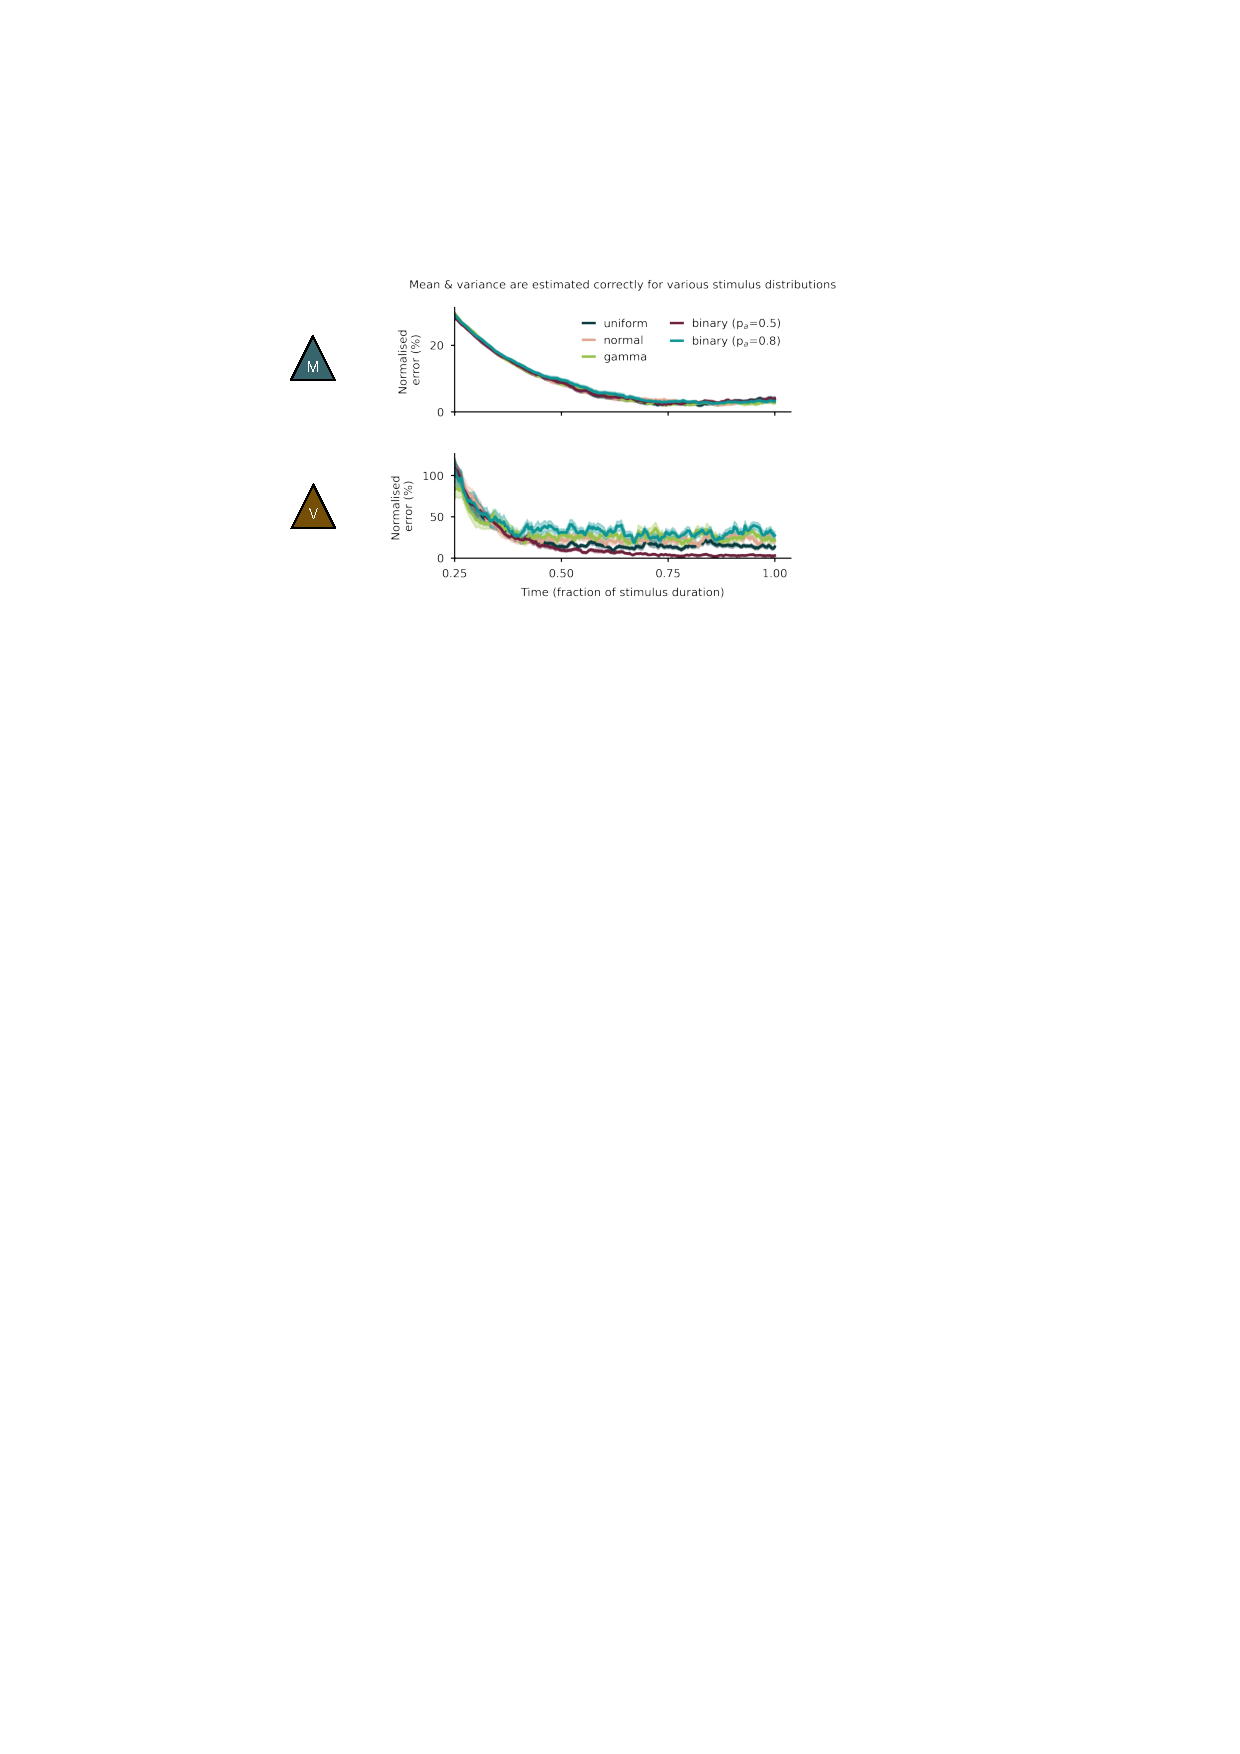
\includegraphics{../results/figures/final/Fig_2_S1.pdf}%DIF >  [width=1\linewidth]
\caption{\footnotesize{\bf Estimating mean and variance of different stimulus distributions.\newline}  
\DIFaddFL{Top: The normalised absolute difference between the averaged mean and the activity of the M neuron decreases to a near-zero level for all stimulus distributions tested. 
Bottom: The normalised absolute difference between the averaged variance and the activity of the V neuron decreases with small differences between the distributions tested. Parametrisation of the uniform distribution as in Fig. \ref{fig:Fig_2}. 
}}
\label{fig:Fig_2_S1}
\end{figure}


\begin{figure}[!h]
	\centering
    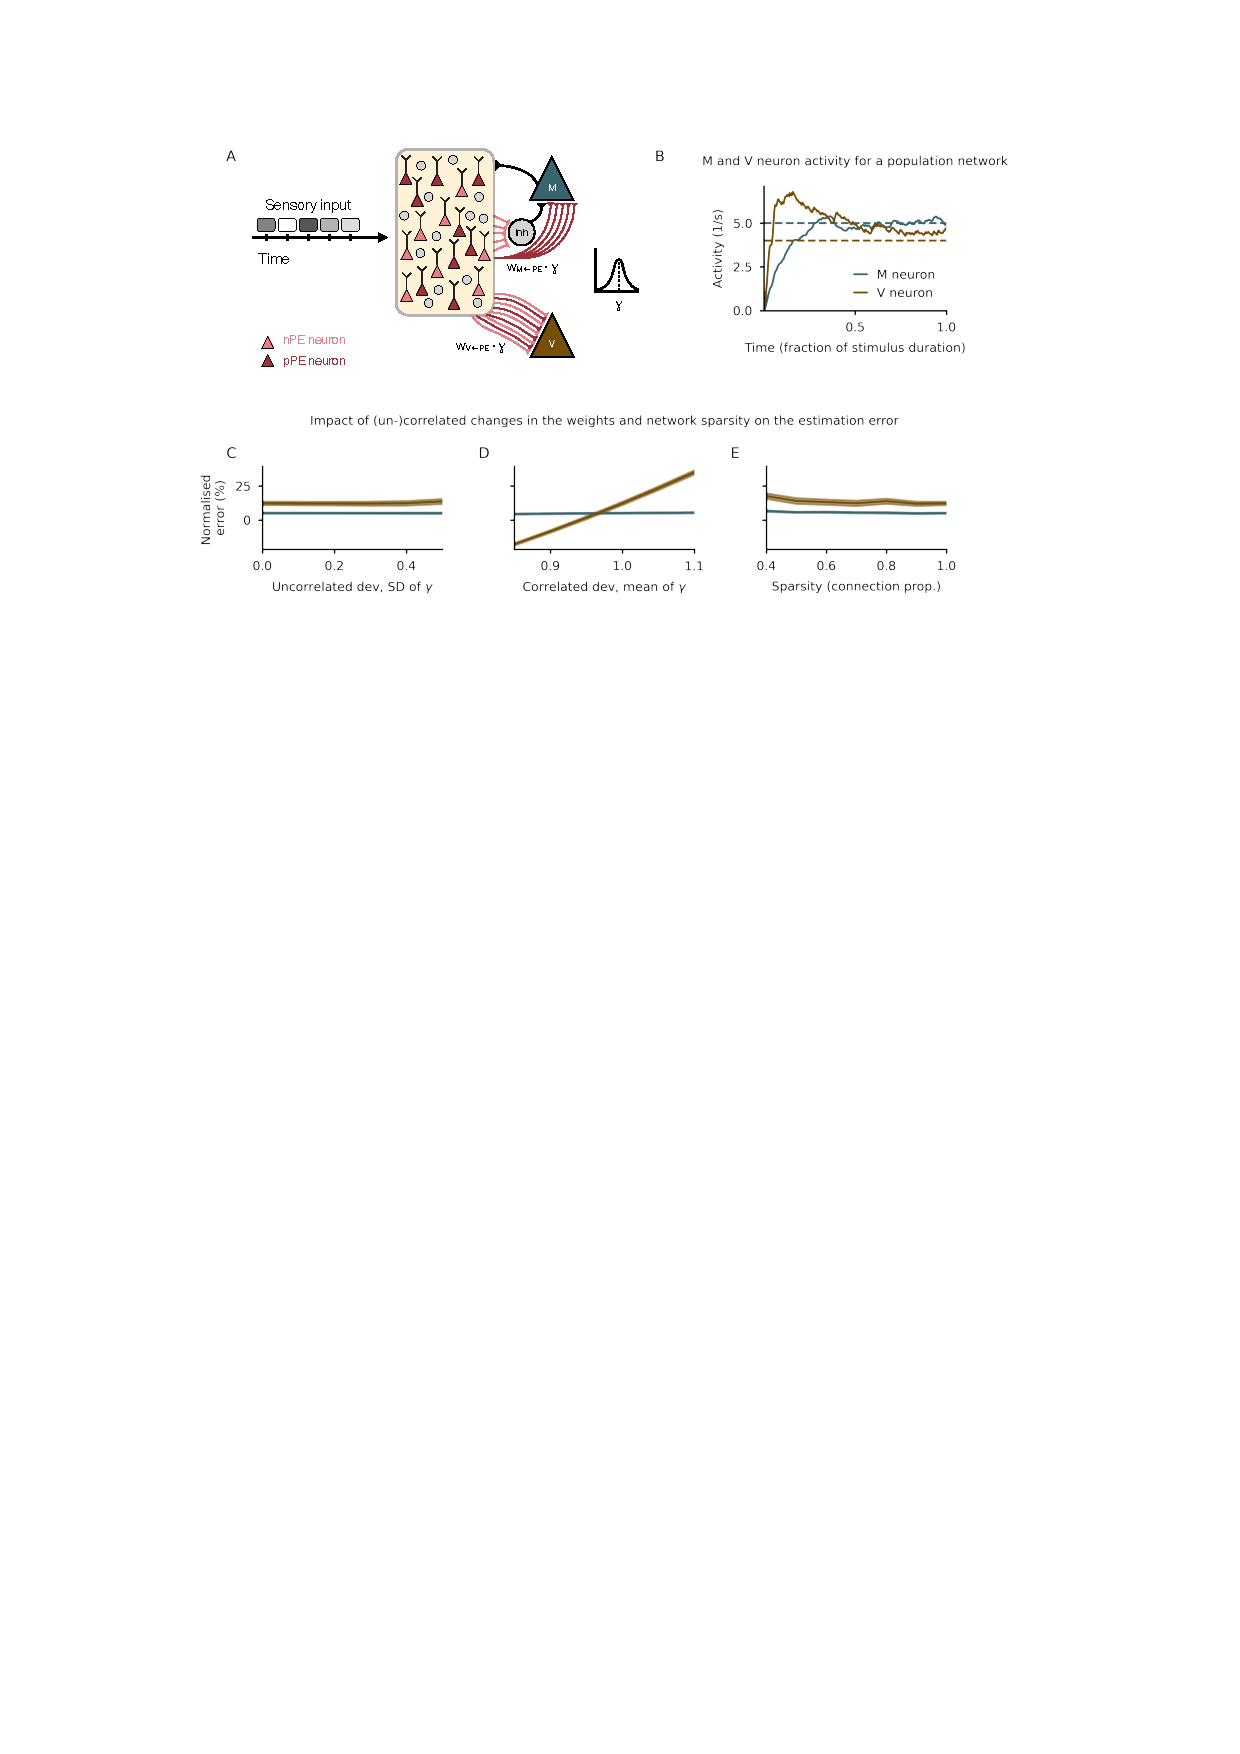
\includegraphics{../results/figures/final/Fig_2_S2.pdf}%DIF >  [width=1\linewidth]
\caption{\footnotesize{\bf Estimating mean and variance of sensory stimuli in a rate-based population network.\newline}  
{\bf \DIFaddFL{(A)}} \DIFaddFL{Illustration of the rate-based population network and the stimuli over time.
}{\bf \DIFaddFL{(B)}} \DIFaddFL{M and V neuron activities over time for one example parameterisation.
}{\bf \DIFaddFL{(C)}} \DIFaddFL{The normalised absolute difference between the averaged mean and the activity of the M neuron (dark green) or between the averaged variance and the activity of the V neuron (brown) for uncorrelated deviations, that is, increasing SD of $\gamma$ (left), correlated deviations, that is, increasing mean of $\gamma$ (middle), and the network sparsity.
}}
\label{fig:Fig_2_S2}
\end{figure}

\begin{figure}[!h]
	\centering
    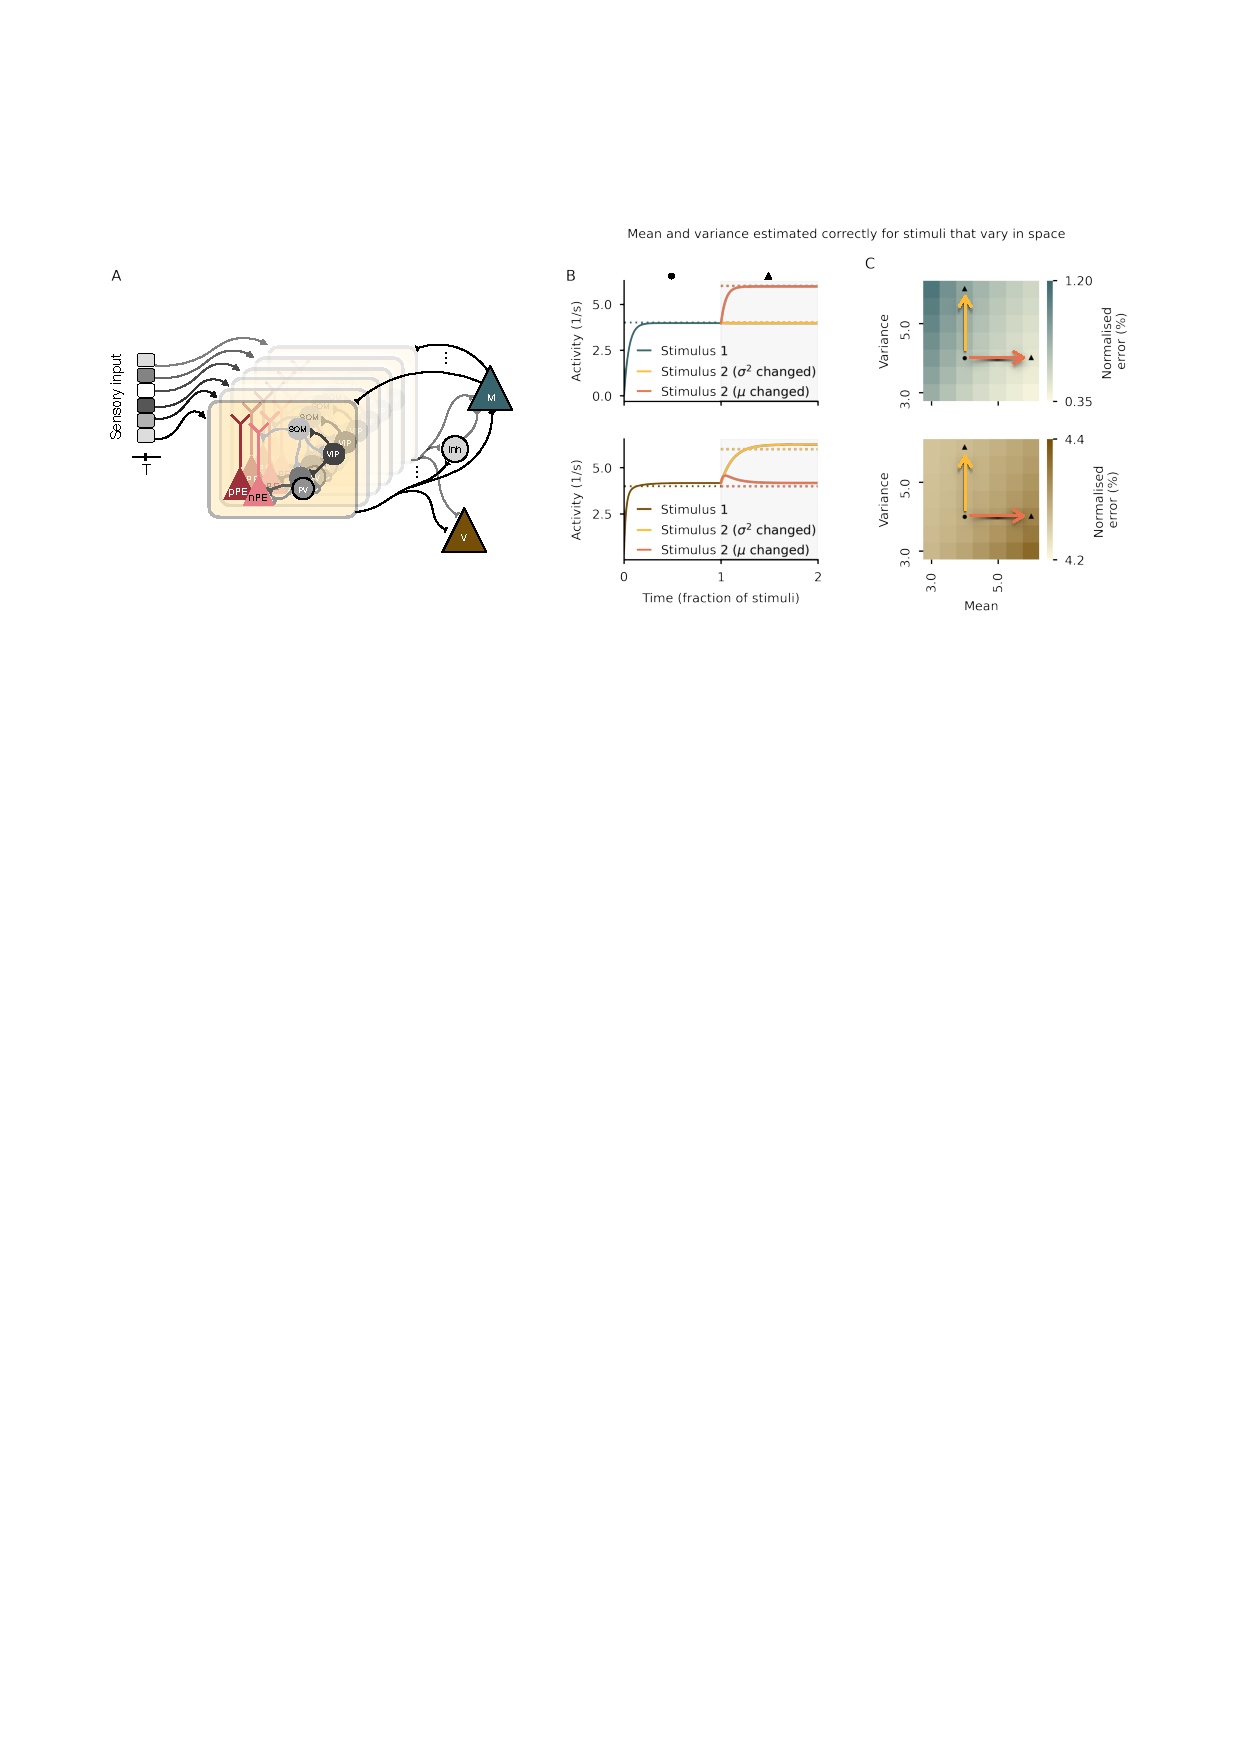
\includegraphics[width=1\linewidth]{../results/figures/final/Fig_2_S3.pdf}%DIF >  [width=1\linewidth]
\caption{\footnotesize{\bf Estimating mean and variance of spatial stimuli.\newline}  
{\bf \DIFaddFL{(A)}} \DIFaddFL{Illustration of a network estimating the mean and variance of a stimulus that varies across space. To simulate selectivity, the network comprises $1000$ identical, uncoupled mean-field networks each receiving a different input value drawn from a uniform distribution. 
}{\bf \DIFaddFL{(B)}} \DIFaddFL{Activity of M neuron (top) and V neuron (bottom) for 2 stimuli. The second stimulus does either differ in the mean (orange) or the variance (yellow) from the first stimulus (indicated in C).
}{\bf \DIFaddFL{(C)}} \DIFaddFL{The normalised absolute difference between the averaged mean and the activity of the M neuron (dark green, top) or between the averaged variance and the activity of the V neuron (brown, bottom) for a range of different stimulus statistics. The examples from B are shown with colored arrows and markers.
}}
\label{fig:Fig_2_S3}
\end{figure}


\begin{figure}[!h]
	\centering
    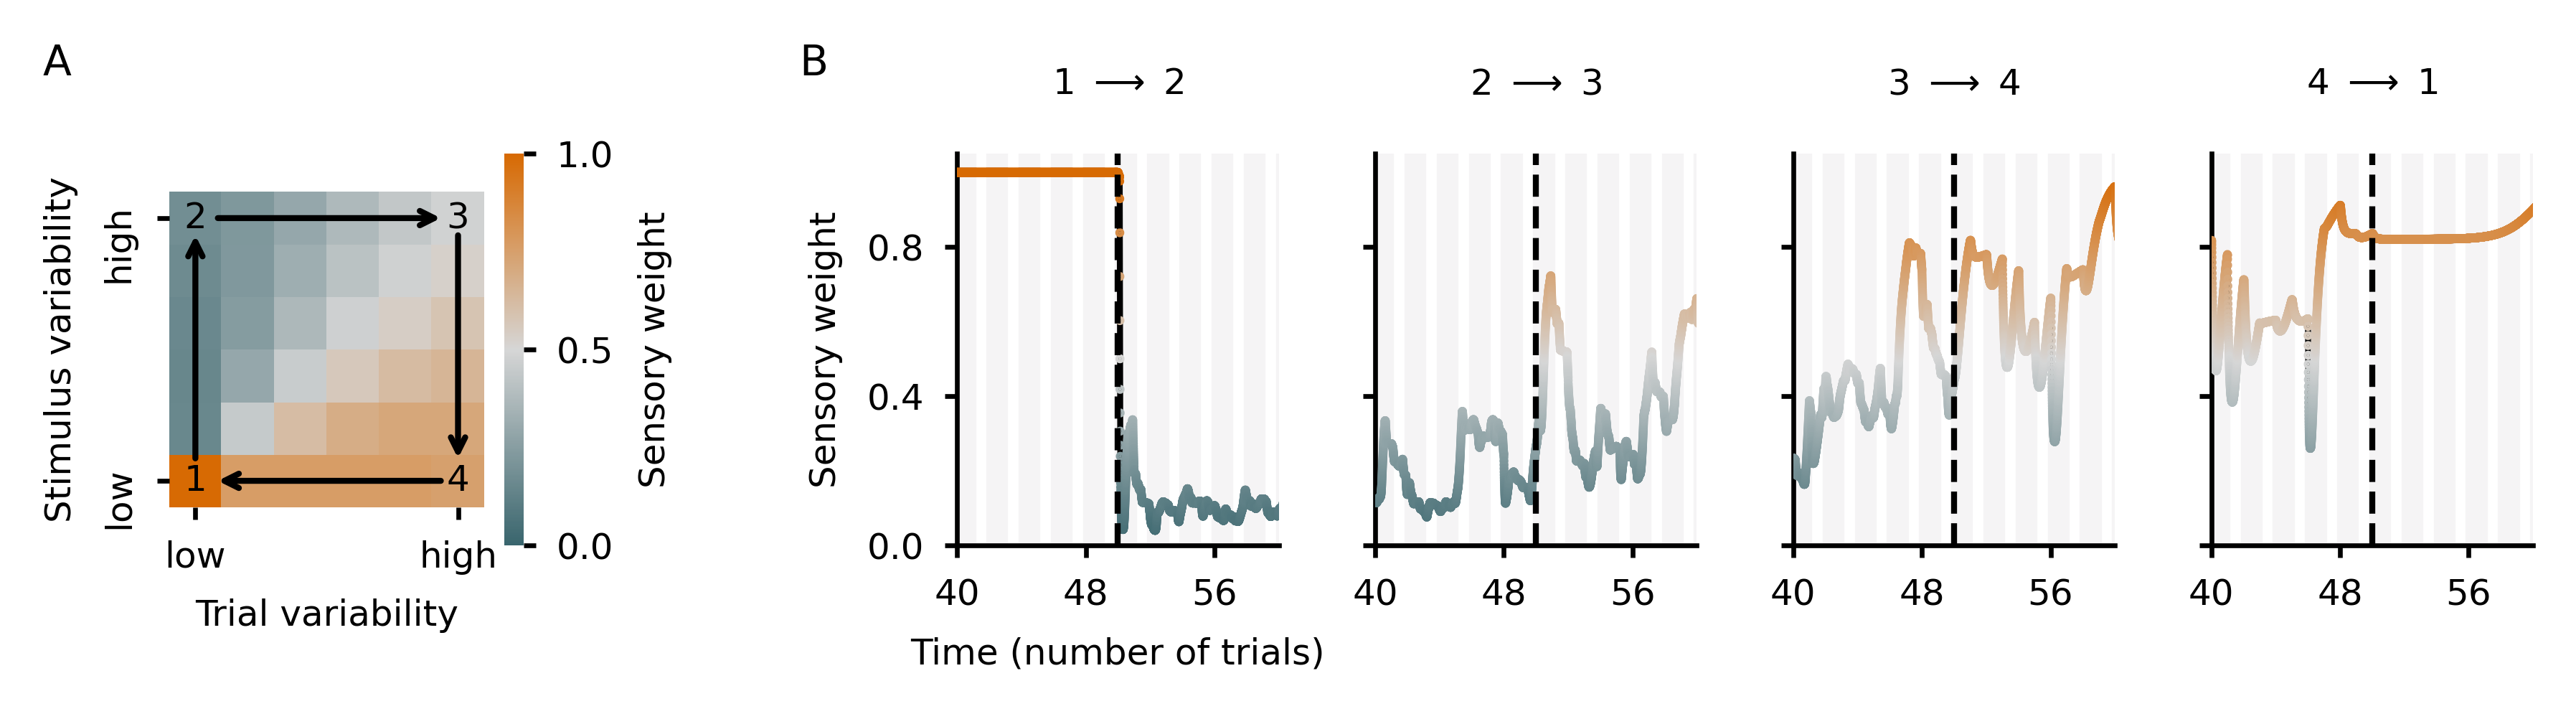
\includegraphics{../results/figures/final/Fig_3_S1}%DIF >  [width=1\linewidth]
\caption{\footnotesize{\bf Dynamic variance estimation allows flexible adaptation to changes in the stimulus statistics and environment. \newline}  
{\bf \DIFaddFL{(A)}} \DIFaddFL{Sensory weight for different input statistics. Numbers denote specific example statistics. Arrows denote the transitions between those statistics.
}{\bf \DIFaddFL{(B)}} \DIFaddFL{The sensory weight over time is shown for all transitions in (A). For the sake of clarity, we only show the trials 40 -60. The switch to new input statistics occurs at trial 50. Parameters are listed in the Supporting Information.
}}
\label{fig:Fig_3_S1}
\end{figure}


\begin{figure}[!h]
	\centering
    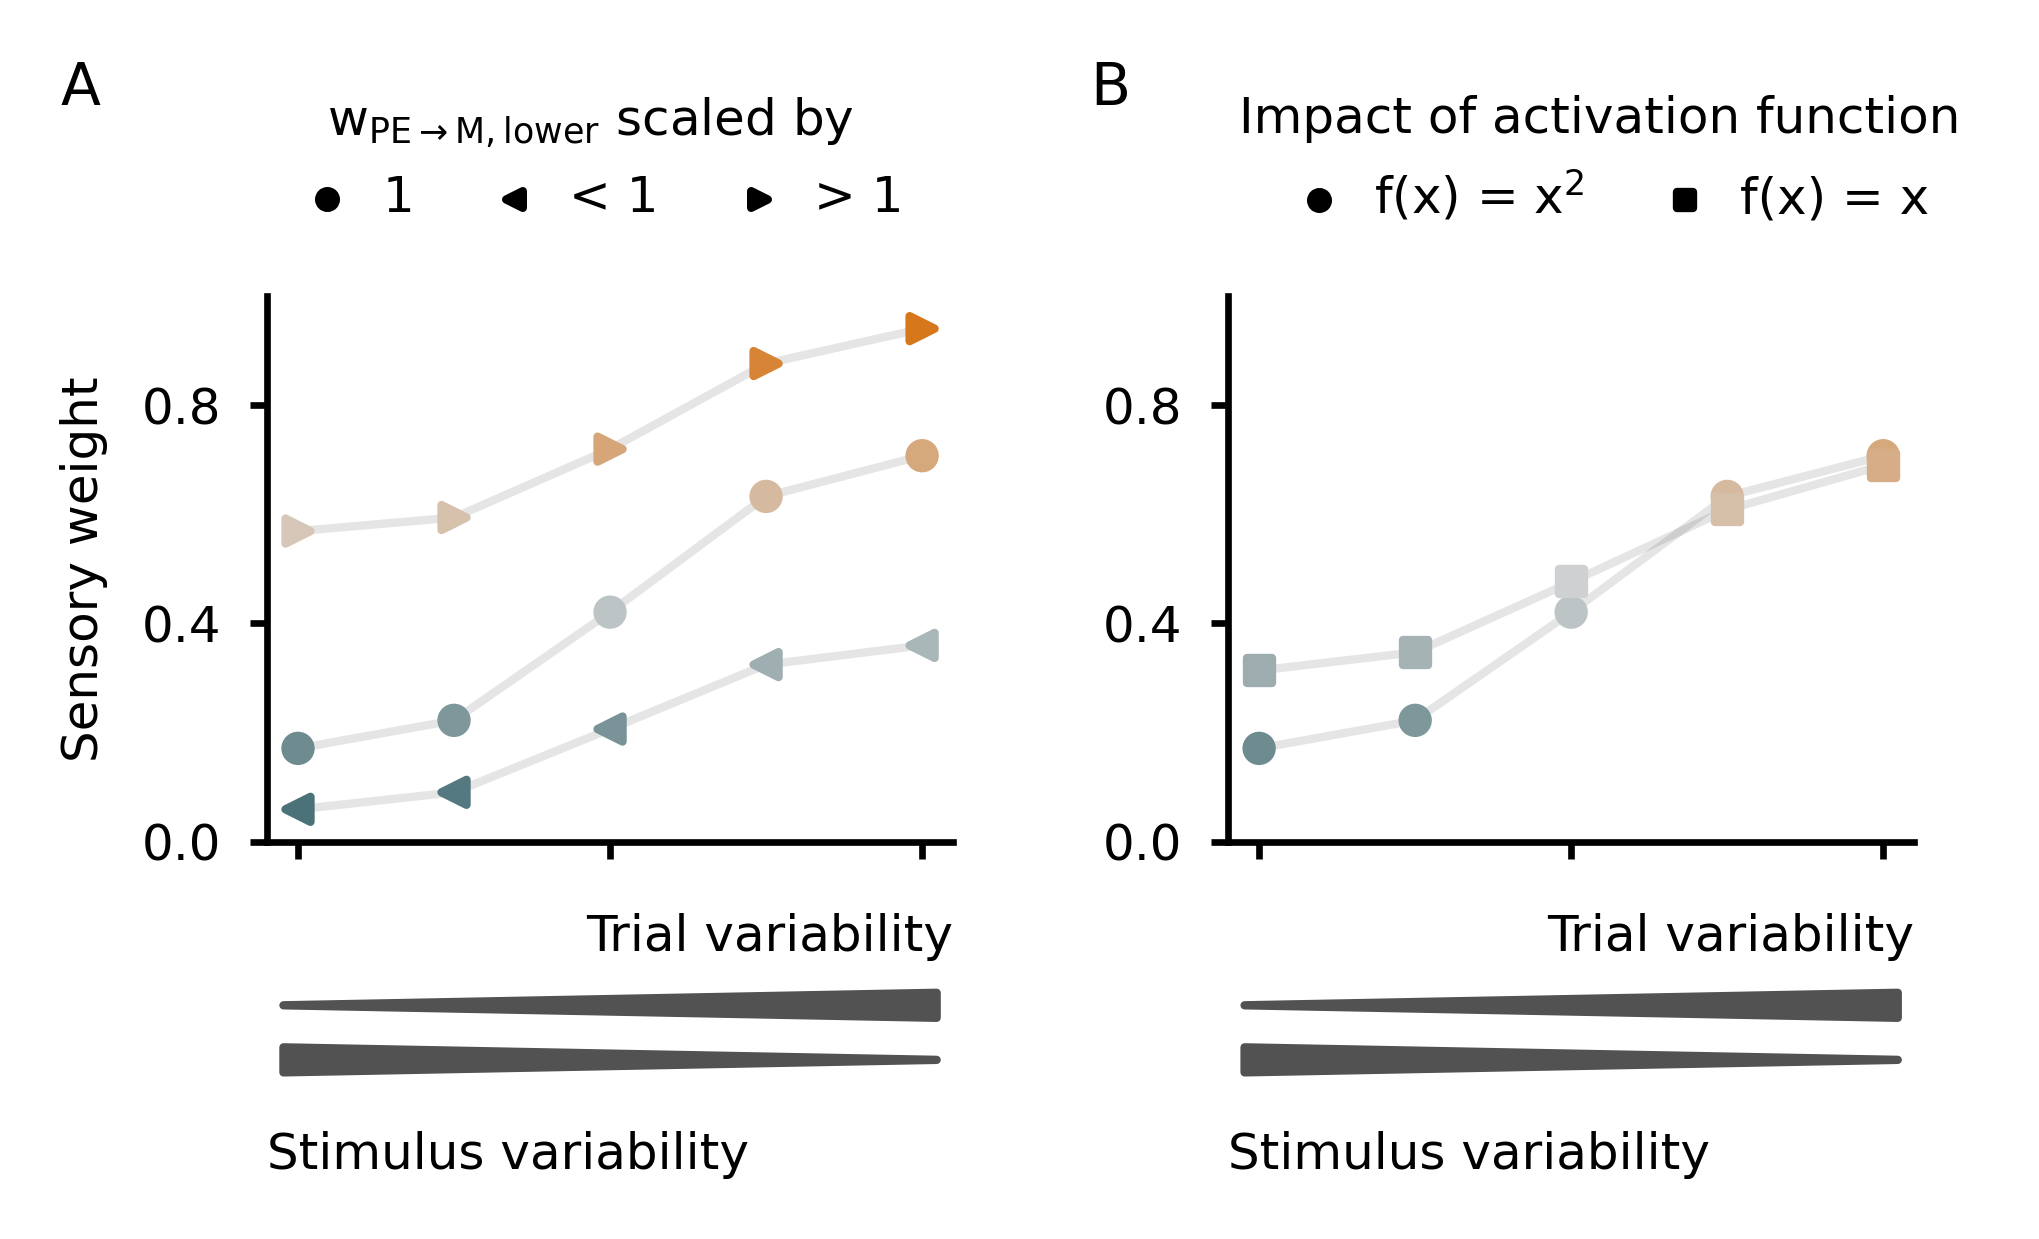
\includegraphics{../results/figures/final/Fig_3_S2}%DIF >  [width=1\linewidth]
\caption{\footnotesize{\bf Perturbing the weighting of sensory inputs and predictions by altering network properties. \newline}  
{\bf \DIFaddFL{(A)}} \DIFaddFL{The weights from the PE neurons to the M neuron in the lower-order subnetwork are scaled by a factor the 0.3 or 7, leading to a distorted sensory weight. If the update of the M neuron in the lower subnetwork is too slow ($\blacktriangleleft$), the prediction is overrated. If the update of the M neuron in the lower subnetwork is too fast ($\blacktriangleright$), the sensory input is overrated.
}{\bf \DIFaddFL{(B)}} \DIFaddFL{The precise activation function for the V neurons does not have a major impact on the sensory weight. Only for inputs with high stimulus variability, the sensory stimulus is slightly overrated when the quadratic activation function is replaced by a linear, rectified activation function.
}}
\label{fig:Fig_3_S2}
\end{figure}


\begin{figure}[!h]
	\centering
    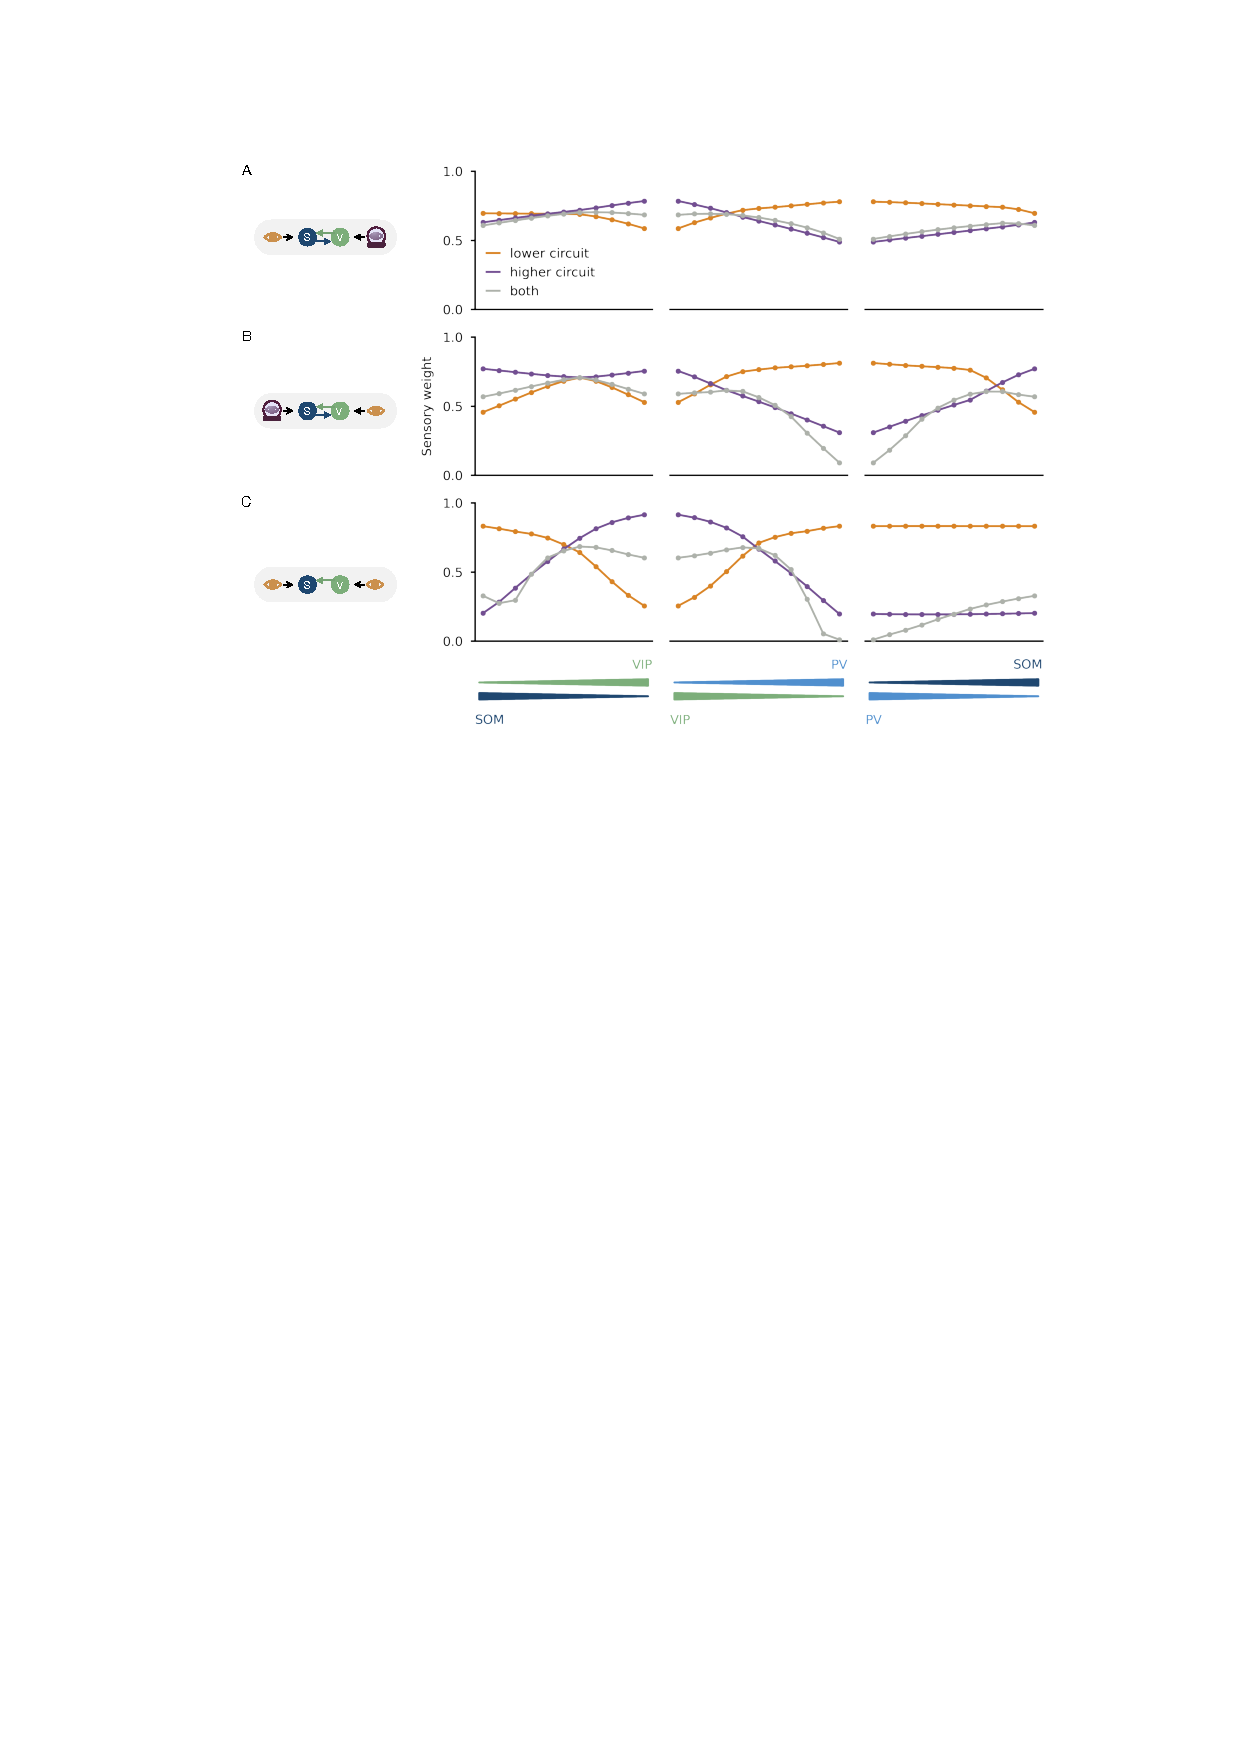
\includegraphics{../results/figures/final/Fig_4_S1.pdf}%DIF >  [width=1\linewidth]
\caption{\footnotesize{\bf The impact of neuromodulators acting globally on groups of interneurons. \newline}  
\DIFaddFL{The sensory weight changes when groups of interneurons are targeted by a neuromodulator. Whether the sensory weight decreases or increases not also depends on the modulation strength (see Fig. \ref{fig:Fig_4}) but also on how strongly which interneuron is targeted.  As shown in Fig. \ref{fig:Fig_4}, the sensory weight is pushed toward 0.5 if the VIP neuron is stimulated. The sensory weight generally decreases when PV neurons are the main target. Considered are two limit cases (upper row: more sensory-driven before modulation, lower row: more prediction-driven before modulation). The results are shown for three mean-field networks (see \ref{fig:Fig_4}).
}}
\label{fig:Fig_4_S1}
\end{figure}


\begin{figure}[!h]
	\centering
    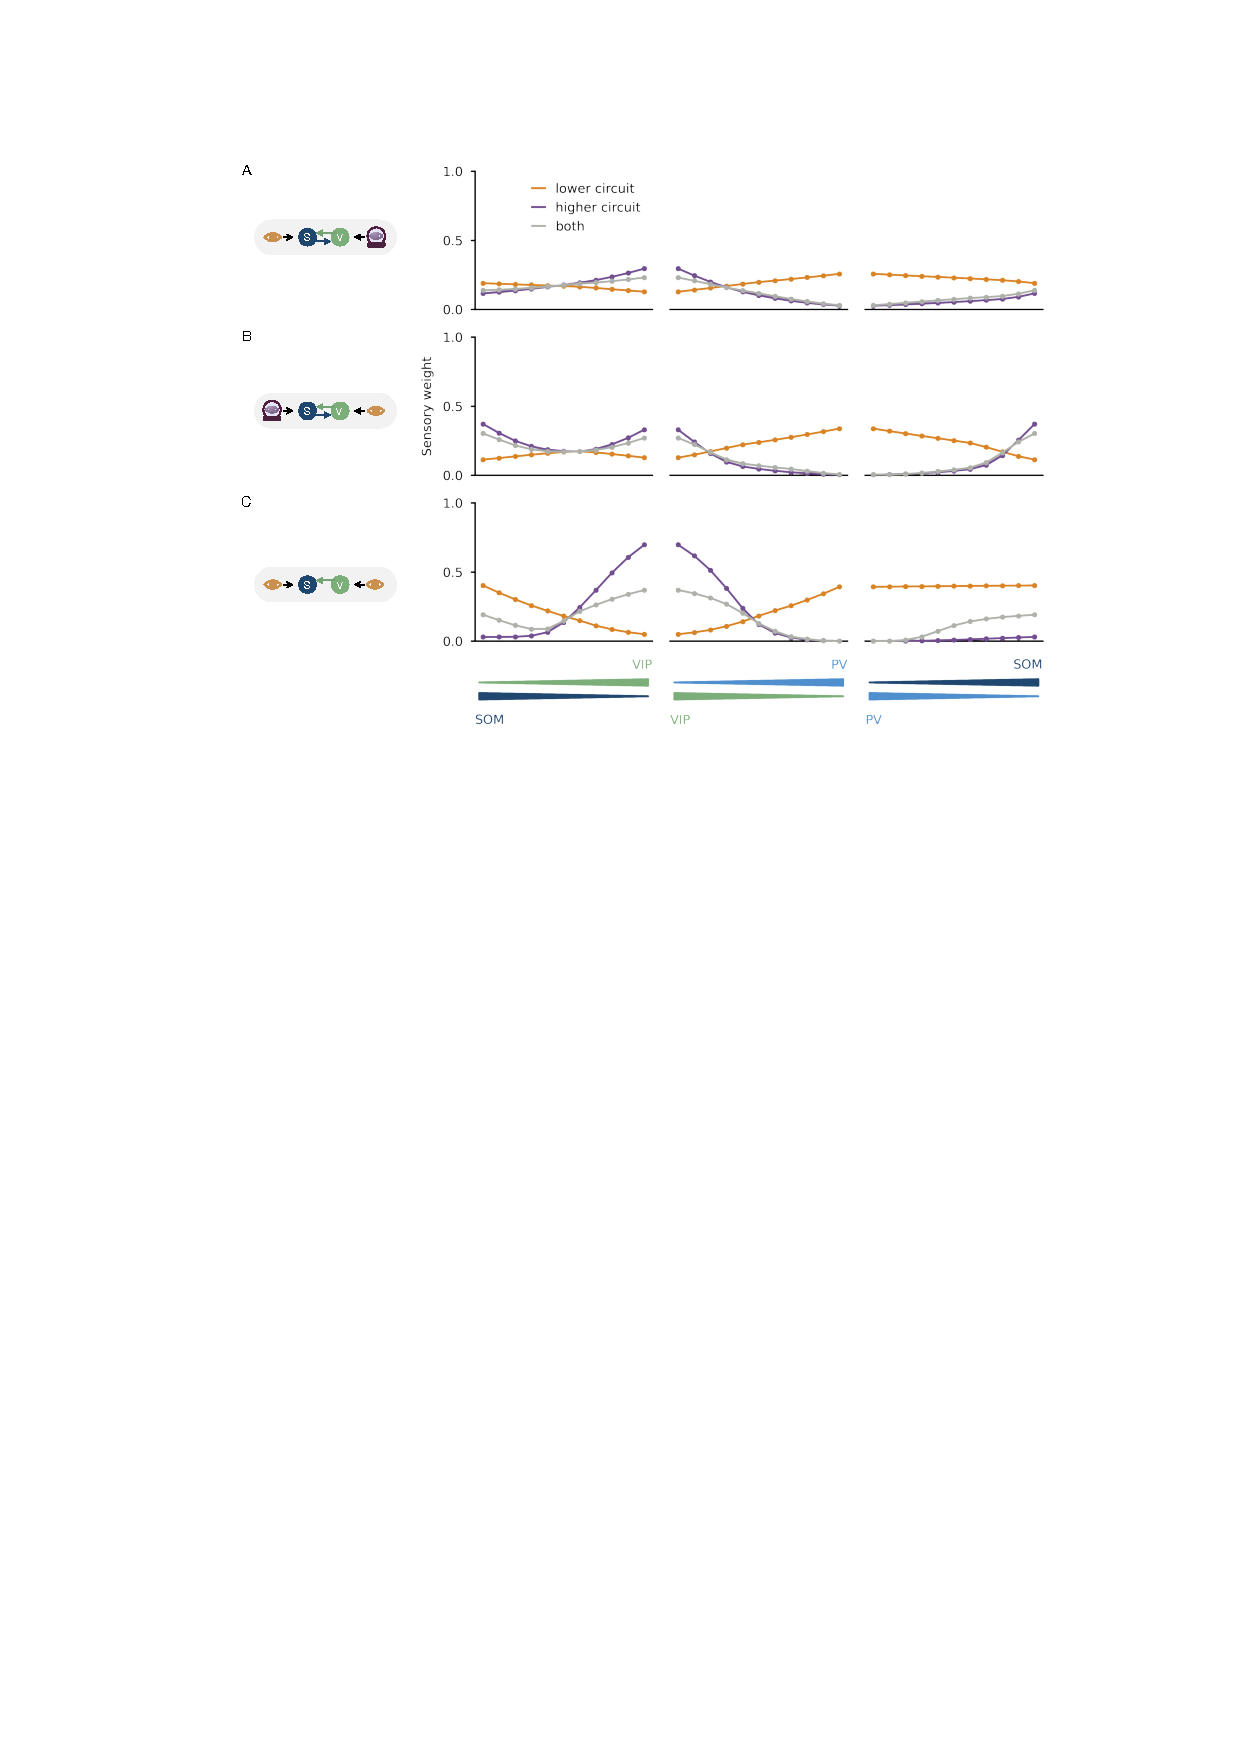
\includegraphics{../results/figures/final/Fig_4_S2}%DIF >  [width=1\linewidth]
\caption{\footnotesize{\bf The impact of neuromodulators acting locally on groups of interneurons. \newline}  
{\bf \DIFaddFL{(A)}} \DIFaddFL{Sensory weight changes with neuromodulators acting on interneurons in the lower PE circuit.
}{\bf \DIFaddFL{(B)}} \DIFaddFL{Sensory weight changes with neuromodulators acting on interneurons in the higher PE circuit. In general, the changes in the sensory weight is the opposite of the changes seen for neuromodulators acting on the lower-level PE neurons. Simulation parameters, labels and colors as in Fig. \ref{fig:Fig_4}. 
}}
\label{fig:Fig_4_S2}
\end{figure}


\begin{figure}[!h]
	\centering
    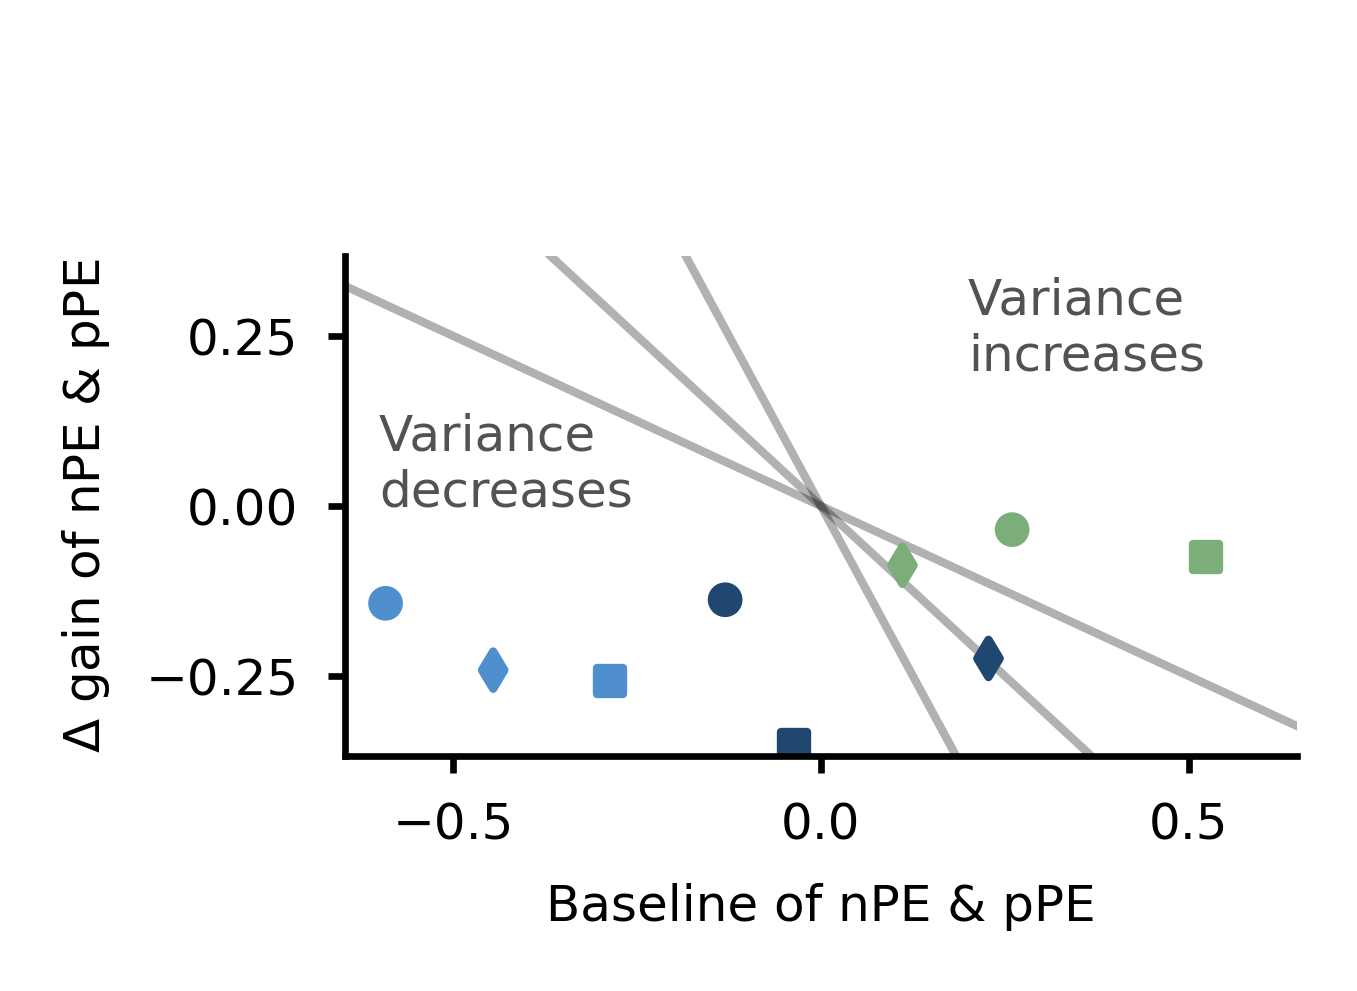
\includegraphics{../results/figures/final/Fig_4_S3}%DIF >  [width=1\linewidth]
\caption{\footnotesize{\bf Biased mean and variance estimation by changing the baseline and the gain of nPE and pPE.}
\DIFaddFL{In a toy model, described in sections \ref{sec:gain_impact} and \ref{sec:impact_baseline}, the contribution of gain and baseline to the changes in the mean and variance estimation are summarized. The results are based on the Eqs. (\ref{eq:prediction_gain}), (\ref{eq:variance_gain}), (\ref{eq:condition_baseline_mean_1}) and  (\ref{eq:condition_baseline_variance_2}).
}}
\label{fig:Fig_4_S3}
\end{figure}

\begin{figure}[!h]
	\centering
    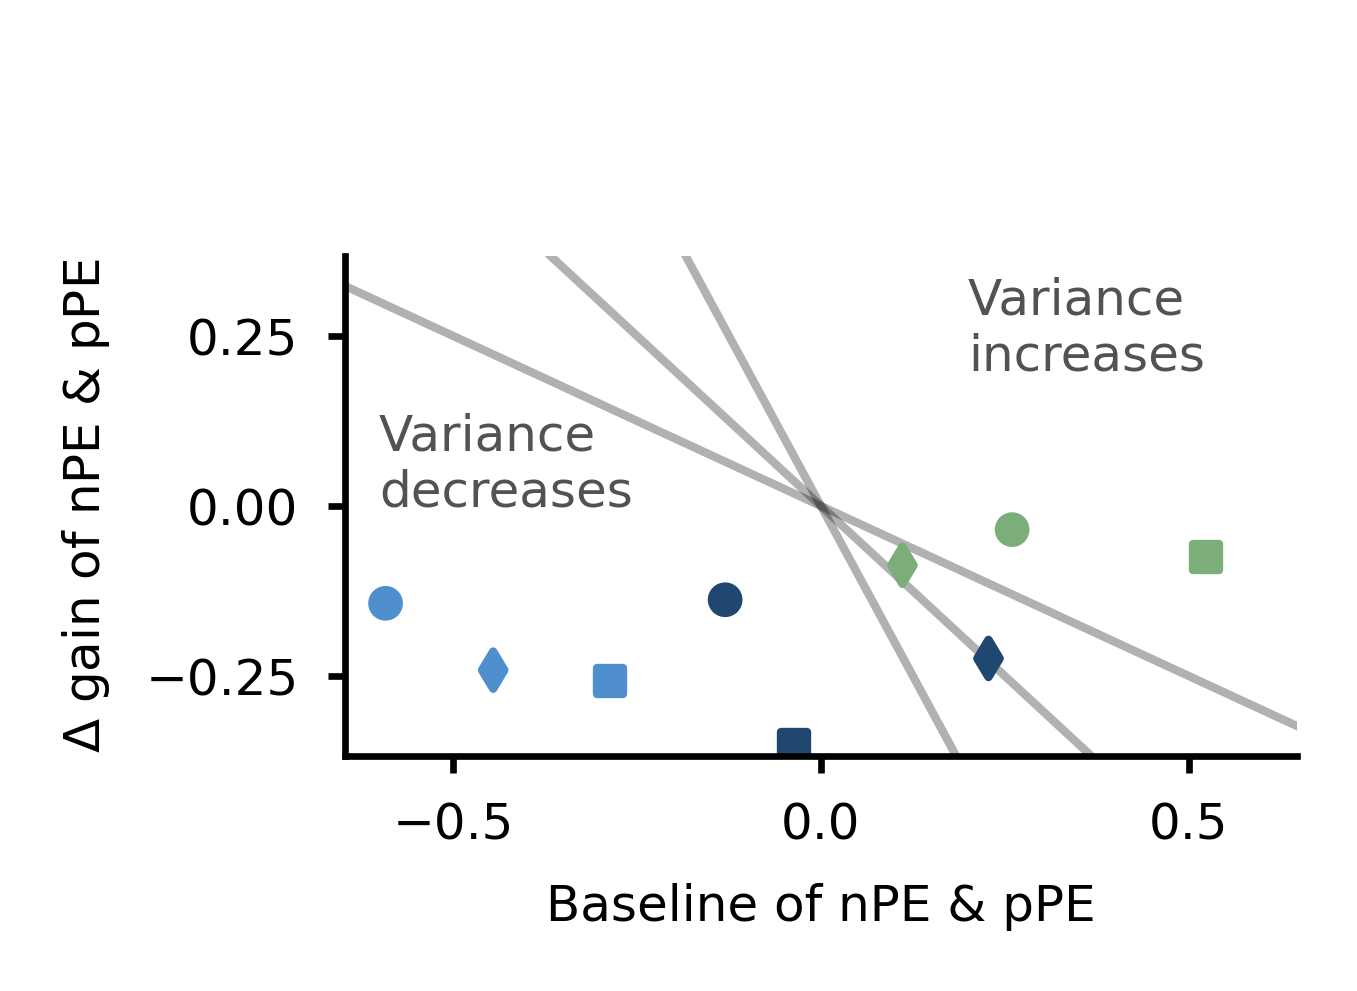
\includegraphics{../results/figures/final/Fig_4_S4}%DIF >  [width=1\linewidth]
\caption{\footnotesize{\bf The combined changes in baseline and gain of all PE neurons determine the shift in the snesory weight.\newline}  
\DIFaddFL{Whether and how a neuromodulator changes the sensory weight depends on the interneuron targeted and the effect this interneuron has on the baseline and gain of both PE neurons, which in turn does depend on the network it is embedded in. For small inputs, changes in the baseline dominate, while for large inputs, the changes in the gains dominate the shift in the sensory weight.
}}
\label{fig:Fig_4_S4}
\end{figure}


\begin{figure}[!h]
	\centering
    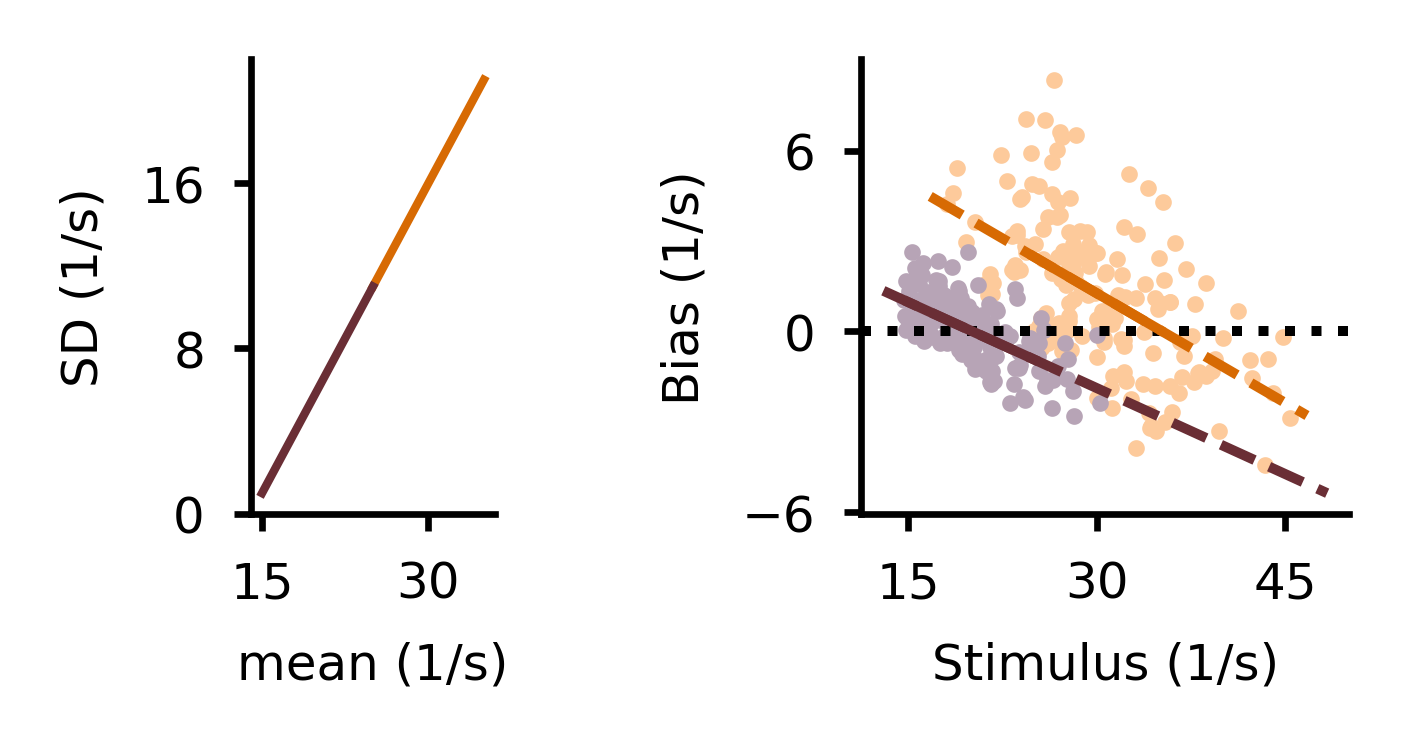
\includegraphics{../results/figures/final/Fig_5_S1}%DIF >  [width=1\linewidth]
\caption{\footnotesize{\bf Including scalar variability in the model \newline}  
\DIFaddFL{When scalar variability is included, that is, the stimulus standard deviation depends linearly on the stimulus mean, the bias is larger for stimuli drawn from the upper end of the stimulus distribution than from the lower end. 
}}
\label{fig:Fig_5_S1}
\end{figure}
\DIFaddend 


\end{document}
